%! TeX program = lualatex

% This is a template for Ph.D. dissertations in the UCI format.
% 
% All fonts, including those for sub- and superscripts, must be 10
% points or larger.  Recommended sizes are 14-point for chapter
% headings, 12-point for the main body of text and figure/table
% titles, and 10-point for footnotes, sub- and super-scripts, and text
% in figures and tables.
%
% Notes: Add short title to figures, sections, via square brackets,
% e.g. \section[short]{long}.
%
\documentclass[12pt,fleqn,hyphens]{ucithesis}
\usepackage{inputenc}
\usepackage{biblatex-chicago}
\addbibresource{thesis.bib}
\usepackage{csquotes}

%% DARK MODE FOR EDITING - OBVIOUSLY COMMENT OUT FOR FINAL
%\usepackage{xcolor}
%\pagecolor[rgb]{0.216, 0.231, 0.271} %blue-dark-grey
%\color[rgb]{0.878, 0.898, 0.949} %blue-light-grey

%% DE-COMMENT TO ALLOW HELVETICA
% \usepackage[scaled]{helvet}
% \renewcommand\familydefault{\sfdefault} 
% \usepackage[T1]{fontenc}

%%%%%%%%%%%%%%%%%%%%%%%%%%%%%%%%%%%%%%%%%%
%%%%%%%%%%%%%%%%%%%%%%%%%%%%%%%%%%%%%%%%%%
% PACKAGES I ADDED %%%%%%%%%%%%%%%%%%%%%%%
%%%%%%%%%%%%%%%%%%%%%%%%%%%%%%%%%%%%%%%%%%
%%%%%%%%%%%%%%%%%%%%%%%%%%%%%%%%%%%%%%%%%%

%----------------------------------------------------------------------------------------
%	USER-PROVIDED PACKAGES AND OTHER DOCUMENT CONFIGURATIONS
%----------------------------------------------------------------------------------------

\usepackage[final]{pdfpages}

% \usepackage{parskip}
% \setlength{\parindent}{48pt}

% Ignores warnings related to package {sectsty} which gets worried
% about these two commands for some reason.
\usepackage{silence}
\WarningFilter[temp]{latex}{Command \underbar has changed.}
\WarningFilter[temp]{latex}{Command \underline has changed.}

% Changes the way urls break across lines. Also the {tt} renders urls in monospaced fonts.
\usepackage{url}
\urlstyle{tt}

%% Set tt font size with \setttsize{\small}, etc.
%The problem is it makes all the tt fonts in footnotes larger...
%\usepackage{letltxmacro}
%% https://tex.stackexchange.com/q/88001/5764
%\LetLtxMacro\oldttfamily\ttfamily
%\DeclareRobustCommand{\ttfamily}{\oldttfamily\csname ttsize\endcsname}
%\newcommand{\setttsize}[1]{\def\ttsize{#1}}%
%\setttsize{\small}

% ALLOWS \overset and \underset COMMANDS as well as \lozenge in Ch. 2
\usepackage{amsmath}
\usepackage{amssymb}

% ALLOWS FOR FUNKY ARROWS IN CH. 3
\usepackage{fdsymbol}
\newcommand{\nwsearrownew}{\mathrel{\text{$\nwarrow$\llap{$\searrow$}}}}

% ALLOWS ``obsessive voice'' ARROW IN CH 3.
\usepackage{utfsym}

% ALLOWS FOR RADULESCU'S FUNKY ALPHA CHARACTER IN CH. 3
\newcommand{\newalpha}{
                        
\includegraphics{images/chapter3/newalpha.png}
                        }

% ALLOWS NICE COLORS
%\usepackage[dvipsnames]{xcolor}

% ALLOWS UPRIGHT GREEK LETTERS
\usepackage{upgreek}

% ALLOWS NICE COLORS
% \usepackage[dvipsnames]{xcolor}
% \usepackage{utfsym}
% \newcommand{\Radulescu}{Rădulescu }

% MORE ADVANCED TABLE PACKAGE
\usepackage{tabularray}

% ALLOWS MULTIPLE IMAGES SIDE BY SIDE IN ONE FIGURE
%\usepackage{subfig}
\usepackage{subcaption}

% ALLOWS NICE TEXT FRAMING
 \usepackage[framemethod=TikZ]{mdframed}

% DEFINES \RAGGEDLEFT \RAGGEDRIGHT ETC.
\usepackage{ragged2e}

% % ALLOWS GOOD CITATION PRACTICES
% \usepackage[useibid]{biblatex-chicago}
% \addbibresource{mybib.bib}
% \usepackage{csquotes}

% DON'T INCLUDE LANGUAGE INFORMATION IN CITATIONS
\DeclareListFormat{language}{}
\AtEveryBibitem{\clearlist{language}}

% BETTER SPACED QUOTE ENVIRONMENT
\usepackage[vskip=5pt]{quoting}

% FIXES CAPTIONS AND ALLOWS FOR CAPTION OPTIONS
\usepackage[margin=10pt,font=small,labelfont=bf]{caption}

% I think I included babel to allow some german bits.
% But then I had to add this command afterward to change the
% contents page to ``table of contents''
%\usepackage[english]{babel} 


% ALLOWS URL BREAKS AT ANY ALPHANUMERIC CHAR
%\usepackage{xurl}

% "Subliminal refinements towards typographical perfection"
\usepackage{microtype}

% IMPROVES FLOATING BEHAVIOR OF FIGURES ETC.
\usepackage{float}
\floatplacement{figure}{H}
\floatplacement{table}{H}
% \usepackage{float}
% \floatplacement{figure}{h}
% \floatplacement{table}{h}

% ALLOWS CHANGES OF LINE SPACING
\usepackage{setspace}

% ALLOWS OPTIONAL ARGS FOR \includegraphics
% type1cm, lettrine allow drop caps
\usepackage{graphicx, type1cm, lettrine}
\graphicspath{ {./images/chapter4/} }

% ALLOWS USE OF EPIGRAPHS
\usepackage{epigraph}
\setlength\epigraphwidth{.55\textwidth}

% ALLOWS FOR WRAPPING TEXT AROUND FIGURES
\usepackage{wrapfig}

% ALLOWS USE OF FRAMES AROUND TEXT/FIGURES which can break across pages
\usepackage{framed}

\usepackage{endnotes}
%\usepackage[hyphens]{url}
%\usepackage[T1]{fontenc}

% ALLOWS USE OF LILYPOND EXCERPTS
\usepackage{lilyglyphs}
\usepackage{fontspec} % ALLOWS ADVANCED FONT SELECTION; ALSO REQUIRED FOR LILYGLYPHS TO WORK FOR SOME REASON

%\setmonofont{Latin Modern Mono Prop Light}[Scale=MatchLowercase]
%\setmonofont{Ricty Diminished}[Scale=MatchLowercase]
\setmonofont{InconsolataN}[Scale=MatchLowercase]

%% BETTER TT FONT (REQUIRES FONTSPEC)
%\setmonofont[ItalicFont=NewCMMono10-Italic.otf,%
%BoldFont=NewCMMono10-Bold.otf,%
%BoldItalicFont=NewCMMono10-BoldOblique.otf,%
%SmallCapsFeatures={Numbers=OldStyle}]{NewCMMono10-Regular.otf}

    % SET MAIN FONT(S) HERE OR COMMENT OUT FOR DEFAULTS
    % THESE ARE JUST SOME FONTS I KIND OF LIKE
    % \setmainfont{IBM Plex Sans}
    % \setmainfont{Cormorant Garamond}
    % \setmainfont{Gentium}

% "Control layout of itemize, enumerate, description"
% This is set in the .cls file
%\usepackage[shortlabels]{enumitem}

\setlist{  
  listparindent=\parindent,
  parsep=0pt,
}

% This makes nicer looking inset quotes, I think. Not necessary
\newenvironment{smallquote}
    {    \begin{quoting}[indentfirst=false]
    \begin{singlespace}
    \small
    }
   { 
   \end{singlespace}
   \end{quoting}
   \normalsize
    }

% PROVIDES ENVIRONMENT FOR \begin{notestuff} and \begin{uselater}
            
\newenvironment{notestuff}{
    \begin{mdframed}[
                    backgroundcolor=red!10,
                    roundcorner=5pt,
                    middlelinecolor=red,
                    middlelinewidth=2pt,
                    leftmargin=2cm,
                    rightmargin=2cm
                    ]
    \vspace{-5pt}
    \small
    \begin{singlespace}
    }
    {
    \end{singlespace}
    \end{mdframed}
    }

\newenvironment{uselater}{
    \begin{mdframed}[
                    backgroundcolor=blue!10,
                    roundcorner=5pt,
                    middlelinecolor=blue,
                    middlelinewidth=2pt,
                    leftmargin=1.5cm,
                    rightmargin=1.5cm
                    ]
    \vspace{-5pt}
    \small
    \begin{singlespace}
    }
    {
    \end{singlespace}
    \end{mdframed}
    }
    
%COMPLICATED PACKAGE FOR BUILDING YOUR OWN GRAPHICS
%UNCOMMENT FOR FINAL
\usepackage{tikz}
    \usetikzlibrary{arrows,positioning,patterns,shapes}

    % ALLOWS FOR CONTOURS AROUND TEXT
    \usepackage[pdftex, outline]{contour}
    \contourlength{1.2pt}
    
% ALLOWS DOTTED OR DASHED VERTICAL LINE
%% EXAMPLE : Text\myline Text\myline[dashed]Text\myline[dotted]
\newcommand\myline[1][]{%
  \,\tikz[baseline]\draw[very thick,#1](0,-\dp\strutbox)--(0,\ht\strutbox);\,%
}

% HIERARCHY DIAGRAM
\usepackage[edges]{forest}

% "Generic symbols for both text and math mode"
% \usepackage{gensymb}

% ALLOWS ARITHMETIC IN LATEX ARGS
\usepackage{calc}

% I DON'T REMEMBER WHAT THIS DOES
\newlength\myheight
\newlength\mydepth
\settototalheight\myheight{Xygp}
\settodepth\mydepth{Xygp}
\setlength\fboxsep{0pt}

% DEFINES ALL GREEK CAPITALS
\usepackage{unicode-math}
\setmathfont{XITS Math}
\setmathfont[version=setB,StylisticSet=1]{XITS Math}

% PREVENTS UGLY SPLITTING OF FOOTNOTES
\interfootnotelinepenalty=10000

% ALLOWS USE OF LILYPOND EXAMPLES DIRECTLY
\usepackage{lyluatex}

% ALLOWS FOR TREE DIAGRAMS
\usepackage{qtree}

% LITERALLY JUST TO PRINT A CURLY X
\usepackage{mathrsfs}

% FOR SOME REASON ONLY INCLUDING THIS PACKAGE {tocloft} ALLOWS THE LISTS OF FIGURES AND TABLES TO SHOW UP---IT SEEMS BROKEN OTHERWISE. I MIGHT AS WELL MAKE SURE I DON'T WANT SOME SPECIAL FORMATTING WHILE I'M AT IT...??
\usepackage{tocloft}

\renewcommand{\contentsname}{\hfill \Large TABLE OF CONTENTS \hfill}
\renewcommand{\listfigurename}{\hfill \Large LIST OF FIGURES \hfill}
\renewcommand{\listtablename}{\hfill \Large LIST OF TABLES \hfill}
\renewcommand{\cftaftertoctitle}{\hfill}
%\addto\captionsenglish{%
%\renewcommand{\contentsname}%
%    {\protect\centering\protect\Large TABLE OF CONTENTS}%
%}
%\addto\captionsenglish{%
%  \renewcommand{\listfigurename}%
%    {\protect\centering\protect\Large LIST OF FIGURES}%
%}
%\addto\captionsenglish{%
%  \renewcommand{\listtablename}%
%    {\protect\centering\protect\Large LIST OF TABLES}%
%}



% ALLOWS TITLES TO BE SINGLE-SPACED
\usepackage{sectsty}
\allsectionsfont{\singlespacing}



%%%%%%%%%%%%%%%%%%%%%%%%%%%%%%%%%%%%%%%%%%
%%%%%%%%%%%%%%%%%%%%%%%%%%%%%%%%%%%%%%%%%%
% END OF PACKAGES I ADDED %%%%%%%%%%%%%%%%
%%%%%%%%%%%%%%%%%%%%%%%%%%%%%%%%%%%%%%%%%%
%%%%%%%%%%%%%%%%%%%%%%%%%%%%%%%%%%%%%%%%%%

% % A few common packages
% \usepackage{amsmath}
% \usepackage{amsthm}
% \usepackage{array}
% \usepackage{graphicx}
% \usepackage{natbib}
% \usepackage{relsize}
% \usepackage[titletoc]{appendix}
% \usepackage[lof]{multitoc}

% % Some other useful packages
% \usepackage{caption}
% \usepackage{subcaption}  % \begin{subfigure}...\end{subfigure} within figure
% \usepackage{multirow}
% \usepackage{tabularx}


% Uncomment the following to attempt to enforce Type 1 or TrueType 
% fonts. ProQuest does not want the type 3 fonts used by default as
% of Dec. 2019 - see 
% https://support.proquest.com/articledetail?id=kA01W000000k9o2SAA . 
% If you are unable to embed fonts such as 'Zapf Dingbats' or 
% 'Symbol', try using raster images (.jpg or .png) instead of vector 
%images (.pdf or .eps).
%\usepackage[T1]{fontenc} 

% plainpages=false fixes the "duplicate ignored" error with page counters
% Set pdfborder to 0 0 0 to disable colored borders around PDF hyperlinks
\usepackage[plainpages=false,pdfborder={0 0 0}]{hyperref}

% Uncomment the following line to use the algorithm package,
% which provides an algorithm environment similar to figure and table
% ("\begin{algorithm}...\end{algorithm}"). A list of algorithms will
% automatically be added in the preliminary pages. Note that you
% probably want a package for the actual code to go with this (e.g.,
% algorithmic).
%\usepackage{algorithm}

% Uncomment the following line to enable Unicode support. This will allow you
% to enter non-ASCII characters (such as accented characters) directly without
% having to use LaTeX's awkward escape syntax (e.g., \'{e})
% NOTE: You may have to install the ucs.sty package for this to work. See:
% http://www.unruh.de/DniQ/latex/unicode/
%\usepackage[utf8x]{inputenc}

% Uncomment the following to avoid "widowing", where page breaks cause
% single lines of paragraphs to float onto the next page (this is not
% a UCI requirement but more of an aesthetic choice).
%\widowpenalty=10000
%\clubpenalty=10000

% Modify or extend these at will.
% \newtheorem{theorem}{\textsc{Theorem}}[chapter]
% \newtheorem{definition}{\textsc{Definition}}[chapter]
% \newtheorem{example}{\textsc{Example}}[chapter]

% Macros for title, author, abstract, etc.
\thesistitle{Scoring the Unknown: Rethinking Fixity and Openness in Western Art Music Notation}

%"Dissertation" for PhD, "Thesis" for master's
\documenttitle{Dissertation}

\degreename{Doctor of Philosophy}

% Use the wording given in the official list of degrees awarded by UCI:
% http://www.rgs.uci.edu/grad/academic/degrees_offered.htm
\degreefield{Music}

% Your name as it appears on official UCI records.
\authorname{Isaac Otto Hayes}

% Use the full name of each committee member and full title 
% (e.g. Professor/Associate Professor).
\committeechair{Professor Mari Kimura}
\othercommitteemembers
{
  Professor Amy Bauer\\
  Professor Michael Dessen
}

\degreeyear{2023}

\copyrightdeclaration
{
  {\copyright} {\Degreeyear} \Authorname
}

% If you have previously published parts of your manuscript, you must list the
% copyright holders; see Section 3.2 of the UCI Thesis and Dissertation Manual.
% Otherwise, this section may be omitted.
% \prepublishedcopyrightdeclaration
% {
% 	Chapter 4 {\copyright} 2003 Springer-Verlag \\
% 	Portion of Chapter 5 {\copyright} 1999 John Wiley \& Sons, Inc. \\
% 	All other materials {\copyright} {\Degreeyear} \Authorname
% }

% The dedication page is optional
% (comment out to exclude).
\dedications
{
  To my mother and father.
}

\acknowledgments
{    
    I'd like to thank the members of my dissertation committee, Dr. Amy Bauer, Dr. Michael Dessen, and my committee chair Prof. Mari Kimura for being so forthcoming with their wisdom and experience.

    I would also like to thank advancement committee members Prof. Mark Dresser and Dr. Lisa Naugle, whose incisive commentary and tricky questions early-on in the process helped contour my writing and creative work.

    I would like to thank The Band: Collin Felter, James Ilgenfritz, Steven Lewis, Jo\~{a}o Martins, Matthew Nelson, Bella Pepke, Atticus Reynolds, and Niloufar Shiri as well as my technical supervisors Oliver Brown and Spencer Pepke---without whom I would be playing solo. 

    Certainly not least, I would like to thank Prof. Roscoe Mitchell, Prof. James Fei, and Prof. Fred Frith, who taught me how to learn to be a better musician.
}


% Some custom commands for your list of publications and software.
\newcommand{\mypubentry}[3]{
  \begin{tabular*}{1\textwidth}{@{\extracolsep{\fill}}p{4.5in}r}
    \textbf{#1} & \textbf{#2} \\ 
    \multicolumn{2}{@{\extracolsep{\fill}}p{.95\textwidth}}{#3}\vspace{6pt} \\
  \end{tabular*}
}
\newcommand{\mysoftentry}[3]{
  \begin{tabular*}{1\textwidth}{@{\extracolsep{\fill}}lr}
    \textbf{#1} & \url{#2} \\
    \multicolumn{2}{@{\extracolsep{\fill}}p{.95\textwidth}}
    {\emph{#3}}\vspace{-6pt} \\
  \end{tabular*}
}

% Include, at minimum, a listing of your degrees and educational
% achievements with dates and the school where the degrees were
% earned. This should include the degree currently being
% attained. Other than that it's mostly up to you what to include here
% and how to format it, below is just an example.
%
% CV is required for PhD theses, but not Master's
% comment out to exclude
\curriculumvitae{

\textbf{EDUCATION}
  
  \begin{tabular*}{1\textwidth}{@{\extracolsep{\fill}}lr}
    \textbf{Doctor of Philosophy in} & \\
    \textbf{Integrated Composition, Improvisation, and Technology} & \textbf{2023} \\
    \vspace{6pt}
    University of California, Irvine & \emph{Irvine, CA} \\
    \textbf{Master of Fine Arts in Music Performance and Literature} & \textbf{2018} \\
    \vspace{6pt}
    Mills College & \emph{Oakland, CA} \\
    \textbf{Bachelor of Arts in Psychology and Philosophy} & \textbf{2012} \\
    \vspace{6pt}
    University of Arkansas & \emph{Fayetteville, AR} \\
  \end{tabular*}

% \vspace{12pt}
% \textbf{RESEARCH EXPERIENCE}

%   \begin{tabular*}{1\textwidth}{@{\extracolsep{\fill}}lr}
%     \textbf{Graduate Research Assistant} & \textbf{2007--2012} \\
%     \vspace{6pt}
%     University of California, Irvine & \emph{Irvine, California} \\
%   \end{tabular*}

\vspace{12pt}
\textbf{TEACHING EXPERIENCE}

  \begin{tabular*}{1\textwidth}{@{\extracolsep{\fill}}lr}

    \textbf{Instuctor of Record} & \textbf{2023} \\
    \vspace{6pt}
    \textbf{Teaching Assistant} & \textbf{2020--2023} \\
    \vspace{6pt}
    University of California, Irvine & \emph{Irvine, CA} \\
  \end{tabular*}

% \pagebreak

% \textbf{REFEREED JOURNAL PUBLICATIONS}

%   \mypubentry{Ground-breaking article}{2012}{Journal name}

% \vspace{12pt}
% \textbf{REFEREED CONFERENCE PUBLICATIONS}

%   \mypubentry{Awesome paper}{Jun 2011}{Conference name}
%   \mypubentry{Another awesome paper}{Aug 2012}{Conference name}

% \vspace{12pt}
% \textbf{SOFTWARE}

%   \mysoftentry{Magical tool}{http://your.url.here/}
%   {C++ algorithm that solves TSP in polynomial time.}

}

% The abstract was previously limited to a maximum of 350 words, 
% but the UCI manual at https://etd.lib.uci.edu/electronic/td2e#2.2.1.
% currently does not indicate that there is any word limit for the abstract
\thesisabstract
{
To date, there exists a startling lack of scholarly literature which attempts to systematically address novel notations for improvisers---particularly instances centering syntactically- and semantically- well-defined symbols. This lack of attention may be attributed, at least partially, to unclear definitions at the heart of the discourse and the lack of a rigorous typology of music notations generally. This dissertation, via a multi-pronged strategy, takes steps toward filling this lacuna. Chapter One provides a historical gloss which grounds twentieth- and twenty-first century performer/notation interaction in much earlier models. Here I demonstrate that overarching notions of notational ``fixity'' and ``openness,'' as well as notions of performance fidelity to a scored work are themselves fundamentally historically contingent. In the process, I highlight pivotal signposts in Western notation which mark important paradigm shifts in these conceptual categories. Chapter Two articulates a clear philosophical position with regard to notational semantic content, ``fixed'' and ``open'' notation, and the notion of the open score as first postulated in the 1950s and '60s. Here I challenge what I take to be conceits of the prevailing ``folk semiosis'' of music notation in order to begin developing a more analytically useful notation typology. To this end, I examine writings by Umberto Eco and Pierre Boulez, along with Gy\"{o}rgy Ligeti's newly-translated \selectlanguage{german} \glqq Neue Notation: Kommunikationsmittel oder Selbstzweck?\grqq---by far the most lucid attempt to formulate such a typology. \selectlanguage{english} Chapter Three deploys concepts solidified in the previous chapter in service of a notation-centric analysis of two late-century work complexes: Anthony Braxton's \textit{Composition No. 76} and Horațiu Rădulescu's \textit{Das Andere}/Op. 89 (\textit{``Before the Universe was Born''}). Interrogating these works' related-but-disparate notation schemes grants new insights into notation's ability to mediate performer/composer agencies and to uniquely reflect composers' communities of practice and musico-philosophical commitments. Finally, Chapter Four thoroughly documents the author's efforts to develop and deploy a novel notation scheme for improvising musicians. This includes a discussion of several aspects of the design and preliminary implementation of \{O-G\} notation as well as of its use in a series of creative works intended to demonstrate its range and flexibility. This is followed by a frank assessment of the extent to which it was capable of fulfilling the author's initial desiderata and subsequent design criteria.
}


%%% Local Variables: ***
%%% mode: latex ***
%%% TeX-master: "thesis.tex" ***
%%% End: ***


% Add PDF document info fields
\hypersetup{
	pdftitle={\Thesistitle},
	pdfauthor={\Authorname},
	pdfsubject={\Degreefield},
}

% Uncomment the following to have numbered subsubsections (by default
% numbering goes only to subsections).
%\setcounter{secnumdepth}{4}


% Set this to only select a subset of the includes directives below.
% Very handy to speed up compilation if you're working on a certain
% part of your thesis. It conserves page numbers, references, etc.
% even for non-included files.
%\includeonly{chapter1, chapter2, chapter3, chapter4}
%\includeonly{chapter1}
%\includeonly{chapter2}
%\includeonly{chapter3}
%\includeonly{chapter4}
%\includeonly{appendix}

\begin{document}

% Preliminary pages are always loaded (TOC, CV, etc.)
\preliminarypages

% Include the different components of your thesis, in separate files.
% Using \include allows you to set \includeonly above.

%% ADDED BY ME -- NEEDED TO RESET PARAGRAPH SPACING AFTER PRELIMS
\setlength{\parskip}{0pt}
\setlength{\parindent}{15pt}

%%%%%%%%%%%%%%%%%%%%%%%%%%%%%%%%%%%%%%%%%%%%%%%%%%%%%%%%%%%%%%%%%
\chapter{Openness as Emergent Performance-Mediator in Western Music Notation}

%%%%%%%%%%%%%%%
% START COPY %%
%%%%%%%%%%%%%%%

\epigraph{\singlespacing ``We are still in the era of Guido, since apart from minor variants in notation and didactics his system has been maintained up to the present day.''}{Jos. Smits van Waesberghe, 1951.}

    % \small
    % \begin{itemize}
    %     \item \texttt{\textbf{\textcolor{red}{Red = construction notes}}}
    %     \item \texttt{\textbf{\textcolor{blue}{Blue = I want this somewhere but maybe not here?}}}
    %     \item \texttt{\textbf{\textcolor{ForestGreen}{green = an idea that, to the best of my knowledge, is mine}}}
    % \end{itemize}
    % \normalsize
    
    Just as the dual traditions of musical literacy and o/aurality have coexisted in Western art music since the genesis of score-making, so too have degrees of notational fixity and openness.\footnote{For clarity: I will use the term ``score'' here in a general sense to refer to any printed form of music notation (rather than in its more specific definition as a drawing together of distinct \textit{parts} which together comprise a document for conducting, analysis or perusal).} All musical traditions develop, thrive, and are passed down only by dint of some degree of material fixity which persists from performance to performance. Likewise all performance-oriented traditions are kept alive by virtue of some degree of in-the-moment spontaneity, some variability or incompleteness, which renders each instance of the tradition unique. This dual nature existed, of course, long before printed music did. Though we lack insight into, for instance, the precise nature of ancient Greek \textit{kithara} music, we may rest assured that its associated practice necessarily involved degrees of both constancy and indeterminacy. With the introduction of more thoroughly conveyable/reproducible (and crucially \textit{durable}) musical artifacts in the form of Guidonian notation, however, a fascinating new layer of complexity emerges. Thanks precisely to the durability of these ``scores'' and their many, many descendants, we are now able to peer backward into what is essentially the whole of the Western art music tradition---enabling us to piece together a narrative which demonstrates the ever-changing impact scored materials have had on the aesthetics and structures of agency of our music-making.\footnote{That we broadly consider ``the tradition'' itself to essentially begin with the dawn of scoring practices itself speaks volumes!}

    To be clear, this chapter does not seek to perform an exhaustive reckoning of the varying modes of improvisatory practice in Western art music. Rather, in order to pave the way for the overarching goal of this document---a more nuanced analysis of the \textit{intentionally}-open notation-mediated practices of the twentieth and twenty-first centuries---this chapter will examine a number of score-oriented ``case-studies''  which will lend clarity to our unique position at the tail-end of 1000+ years of this symbiotic oral/literary meta-tradition.

    After outlining some much-needed provisional definitions, this chapter will examine (chronologically) exemplars from what I take to be key models along the long historical arc of our relationship to notational fixity---specifically: (1) the medieval, (2) Renaissance, (3) romantic, (4) Afro-diasporic, and (5) postwar models. Only after this short catch-up will we have the tools needed to elucidate the new (i.e. post-1970) models of musical openness which ultimately concern us.

\section{What is a notation?}

    First, though, it is of the utmost importance that we arrive at a few working definitions. I have thus far used the term ``score'' rather loosely to refer to any durable arrangement of symbols which somehow permit the recollection or performance of a musical work---in contravention, perhaps, of the typical way we imagine a score: a rather rigorous, precise accounting of pitch, rhythm, tempo, timbre, indeed any and all parameters necessary for an accurate rendition of a finished piece of music. Of course, what exactly constitutes ``rigor,'' ``precision,'' and indeed ``finished'' when it comes to a musical work is entirely historically contingent---one of the main thrusts of this chapter. Thus a satisfactory definition should permit some wiggle room as regards these traits.

    I find virtuoso violinist and scholar Mieko Kanno's definition of (classical) music notation to be particularly eloquent and inclusive:

        \begin{smallquote}
        Musical notation in western classical music is a system which preserves past musical events while enabling and informing future ones, both describing musical works and giving specific instructions for them to be realized [...] In general, in classical music, notation is considered to be as important---if not more important than---performance and recording, in learning what we consider to be the essence of a musical work.\autocite{Kanno_2007}
        \end{smallquote}
        
    Though the scope of Kanno's article is limited to a rather narrow subset of scoring practices, namely those pertaining to twentieth-century classical music, her definition surely remains relevant to a broad range of musical paradigms. Notation, as Kanno describes it here, may serve as an archival aid, as a means of jotting down sketches, as an analytic tool, as a necessary precursor to performance, etc.---qualities which remain constant over the entire historical lifespan of the practice. Even more pithily, Floris Schuiling (to whose incisive paper I will return in a future section) defines a  notation---sans qualification---as simply an ``[interface] for imagining virtual musical relations,'' notably omitting any reference to actually-existing materials referenced \textit{by} notation past or present. In some respects this is the safer choice insofar as we'll later encounter notations which stretch Kanno's interpretation of the term, but for the moment I'll split the difference with the following definition:

        \begin{smallquote}
             A \textit{music notation} consists of a coherent set of symbols oriented toward an existing (i.e. past or present) or virtual (i.e. potential future) musical product---sounds organized in time. These symbols, taken together permit or facilitate the recording, analysis, or performance of such products.
        \end{smallquote}


    \noindent Chapter 2 will require some additional refinement of this definition, but for now it will suffice to take us through commonly-understood structures of notation.

    What, then, of this hugely important discrepancy between the ``fixed'' and the ``open'' in music? In Chapter 2 we will look in some detail at Umberto Eco's seminal essay collection \textit{The Open Work} (from whence we get the term). However, for the moment let us consider some instance of musical notation to be ``open'' to the extent that some parameter or parameters remain variable from performance to performance. For instance: the excerpt for keyboard shown in Figure~\ref{fig:nonmesure}, a snippet of a seventeenth-century \textit{prélude non mesuré}, is (relatively) \textit{fixed} with regard to pitch content but remains \textit{open} with regard to duration, rhythm, tempo, attack, etc.\footnote{``Relatively fixed,'' that is, bracketing issues of temperament, central pitch frequency, etc.} The pitches provided present a non-negotiable skeletal framework for performance, the absence of which would render a given realization imprecise or unfaithful. The parameters left open, however, are subject to change from performance to performance, determined by factors such as prevailing notions of ``good taste,'' the performer's musical education or creative will, etc.---factors which will change depending on the cultural conditions surrounding music-making in a given time/place.

        \begin{figure}
            \centering
            \fbox{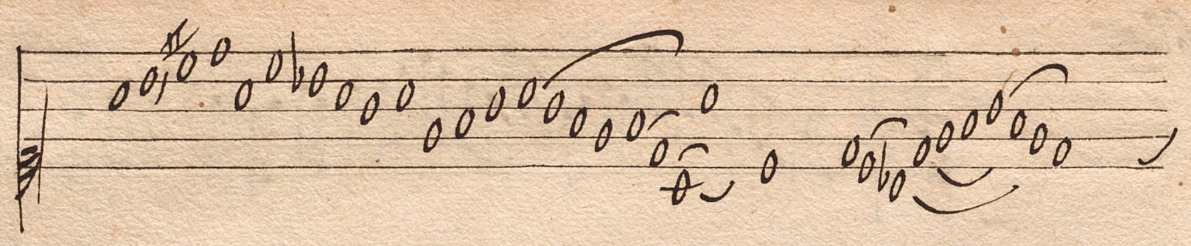
\includegraphics[width=.9\linewidth]{images/chapter1/delanglebert1.png}}
            \captionsetup{width=.5\linewidth}
            \caption[An excerpt from one of Jean Henry D'Anglebert's seventeenth-century unmeasured preludes using the ``whole note'' glyph to represent each pitch ametrically.]{An excerpt from one of Jean Henry D'Anglebert's seventeenth-century unmeasured preludes using the ``whole note'' glyph to represent each pitch ametrically.\footnotemark}
            \label{fig:nonmesure}
        \end{figure}
            \footnotetext{\fullcite{Chung_2019}}

    Thus, our second working definition:

        \begin{smallquote}
        An \textit{``open'' notation} is any notation which requires active creative (i.e. generative) participation on the part of an interpreter to faithfully render the musical product toward which it is oriented.
        \end{smallquote}

    %There is no clearly delineated fact-of-the-matter as to how the ``open'' parameters of the excerpt are to be played. 

    Note that this is \textit{not} to say that these open parameters were, in the seventeenth century, fully unbounded and that any interpretation would suffice, so long as it heeded the aforementioned fixed elements. Rather, ``openness'' in the most generic sense merely points to some degree of indefiniteness or ``incompleteness'' as regards what music, precisely, is represented on the page. Thus, crucially, under this view \textit{every} music notation designed for human interpretation is, in a non-trivial sense, open to some degree. Even the most seemingly stringent and exquisitely detailed forms of notation we find used by the likes of Brian Ferneyhough or Michael Finnissey necessarily leave key aspects of performance up to the taste and experience of the performer.
    
    Ian Pace, in his contribution to \textit{Unfolding Time} (2009), reinforces this notion via his ``negativistic'' account of music notation.   

        \begin{smallquote}
            [The historical construct of music notation \textit{in toto}] is, to my mind, founded upon an essentially \textit{positivistic} view of the role of notation. By this I mean the notion that the score tells the performer in essence \textit{what} to do, around which he can elaborate [...] depending on the degree of notational exactitude. The alternative model I wish to propose draws upon structuralist thinking about language; instead of seeing the score in a \textit{prescriptive sense} [...] I would suggest that instead it delineates the range of possible performance activities by telling the performer what \textit{not} to do. [...]

            \vspace{7pt}
            
            \noindent[I]f a performer thinks of notation in this way, the task becomes less one of playing something `right' as playing it `not wrong'.
        \end{smallquote}

    In short, the boundaries notation imposes on performance are in fact broad zones of exclusion. Per Pace's example, the triplets in Chopin's \textit{Impromptu in G$\flat$}, Op. 51 are fundamentally open in the sense that they permit any interpretation not excluded by their ``triplet-ness.'' Only if a performance departs so greatly from the printed page that the gesture is heard as an entirely different metric grouping does it qualify as unfaithful or ``incorrect''---thus, for Pace, a less detailed notation is a more open notation on account of forbidding fewer interpretations.\autocite[154--6]{Pace_2009} Crucially, though, there is no point of maximum fixity at which \textit{all interpretations but one} are forbidden; ergo, it is possible to meaningfully describe any notation as occupying some point along this axis.
    
    % Per Charles Seeger, the notation to which we are accustomed ``...does not tell us as much about how music sounds as how to make it sound. ... [N]o one can make it sound as the writer of the notation intended unless in addition to a knowledge of the tradition of writing he has also a knowledge of the oral (or, better, aural) tradition associated with it...''\autocite{Seeger_1958}

    For the purposes of this chapter, I'll dub the entire range from some purely theoretical fully-fixed, wholly representative notation to an equally hypothetical fully-open notation the ``fixity gradient.'' While each notation practice examined here will demonstrate fixity/openness in different ways and to different ends, this ``gradient'' might serve as a helpful (if reductive) analytic tool to facilitate greater insights into the way various notations mediate musical performance.

    \section{Notation as archive: Guido d'Arezzo's new fixity}

    We now largely conceive of liturgical notation in medieval Europe as gradually congealing into the four-line-staff form put forward by Guido d'Arezzo in the eleventh century, having originated in pitchless neumes which offered to the cantor only a general notion of melodic contour and syllabic stress.\autocite[16]{Taruskin_2009} While Guido was not the first to take a stab at more precisely encoding sacred melodies using ``heighted'' tones oriented around a central pitch (a practice which, in some form or another, dates at least as far back as Boethius and the ancient Greeks before him\autocite[17]{Taruskin_2009}), Guido's four-line staff facilitated melodic acquisition by allowing singers to more easily visualize the various intervals to be sung and to determine the chant's ``home'' hexachord.\autocite[53]{Reisenweaver_2012} Figure~\ref{fig:guidonew} shows one of a number of techniques Guido demonstrates in the \textit{Micrologus} which more precisely encode melodic contour. While often pitches would be appended to individual syllables, this rendering is looser still in that it gives the cantor no indication of syllabic break-points. The rhythmic indications shown in the inset mensural notation are an anachronistic appendage by a later publisher.

        \begin{figure}
            \centering
            \fbox{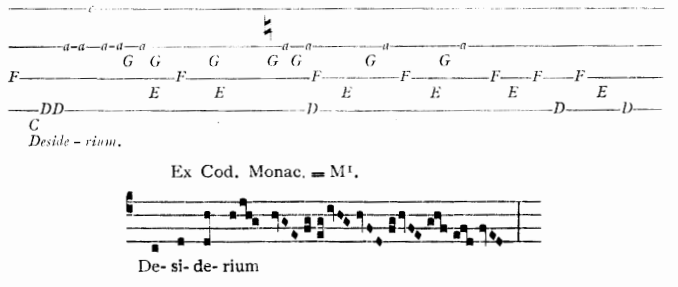
\includegraphics[width=.9\linewidth]{images/chapter1/guido4.PNG}}
            \captionsetup{width=.5\linewidth}
            \caption[A pedagogical excerpt from Guido's \textit{Micrologus} demonstrating the four-line staff with ``heighted'' neumes---shown here both in Guido's original letter notation (above) and in the later ``black note'' mensural notation (added in the 1904 Solesmes edition).]{A pedagogical excerpt from Guido's \textit{Micrologus} demonstrating the four-line staff with ``heighted'' neumes---shown here both in Guido's original letter notation (above) and in the later ``black note'' mensural notation (added in the 1904 Solesmes edition).\footnotemark}
            \label{fig:guidonew}
        \end{figure}
            \footnotetext{\fullcite[28]{Guido_1904}}

    Speaking generally, it was a centuries-long yearning for greater notational fixity---a more substantive relationship between sign-system and sound concept---that motivated this shift from pitchless to pitched neumes. Guido's stated goal, that ``anyone, with the use of the monochord and with careful instruction in the use of our notes, might, at the end of one month, be in a position to sing songs neither seen nor heard before, on the first glance''\autocite[16]{Arezzo_1943} arose explicitly in response to a perceived lack of accuracy in the recitation of traditional music, where previously even ``a hundred years [of] study of songs''\autocite[17]{Arezzo_1943} was insufficient to guarantee fidelity among learned singers.

    %[QUOTE ON NEED FOR NOTATION FROM TARUSKIN]
    %[PG 15 of original BPL194 manuscript: https://digmanclass.universiteitleiden.nl/manuscripts/bpl-194/] = guido2sancte

    In contrast to prevailing forms of concert music notation today, Guido's appears startlingly vague. His novel system (which would reach maturity in the form of the more complex ``black note'' mensural notation of the European Renaissance) demonstrates no rhythmic fixity whatsoever, owing, presumably, to the fact that these melodies were necessarily appended to sacred texts which carried with them their own prosodic rhythms. Similarly we find no specifics regarding pace, quality of voice, number of performers, ornamentation, etc. Referring to his treatise (but applying equally to his newly-developed system), he writes: ``That which in music is of little significance for the art of singing, or which would not be easily understood I have not held worthy of mention.''

    %[[CHANGE THIS SECTION --- FROM GUIDO OF AREZZO AND HIS INFLUENCE ON MUSIC LEARNING]]

    %Figures 2 and 3 below show one of a variety of techniques Guido demonstrates in the \textit{Micrologus} which precisely encode melodic contour\footnote{In this instance Guido is using this \textit{Sancte Iohannes} passage to illustrate one means of illuminating arbitrary liturgical texts using their vowel content}. The highlighted passage appends fixed pitches to each syllable of the text, which are then ``heighted'' to regular degrees above an initial pitch ``C.''

    The extent to which this system appears ``open'' by today's standards, though, should not be taken as an indication that its performers were granted a commensurate degree of creative latitude in its realization. Whereas deliberately open notations in the twenty-first century often serve as tacit invitations on behalf of a composer to bend the finished work to the performers will and experience, Guidonian notation was, from the outset intimately bound up with a robust o/aural tradition oriented toward regular, faithful reproduction of comparatively immutable sacred texts. So rigid and commonly-understood was this tradition, apparently, that Guido saw no need to render details of its execution in his notation, save for the melodies themselves which, on account of their prodigious quantity and the difficulty of their memorization, formed the main pedagogical stumbling-block of his project. 

    Perhaps owing to the notation's aforementioned lack of fixity, regional variation \textit{is} assumed to have cropped up as the new system moved geographically outward.\autocite[466]{Hucke_1980} Additionally, the question of varieties of rhythmic interpretation of plainchant melodies is far from settled. Attempts to uncover ``\textit{the} authentic rhythm of chant''\autocite[319]{Brunner_1982} have largely come up empty, inviting the notion that rhythmic variations between performances formed much of the regional flavor of church music practice. However, this variation clearly arose by virtue of the notation's ``technological'' limitations and the realities of pre-Enlightenment communication rather than from some desire on the part of the notation's architect(s) to draw out these distinctions. Arguably, the miracle of Guidonian notation and its successors lies in the fact that despite such sparse notation, the genre underwent precious little change (melodically, at least) over centuries of practice---perhaps, as Helmet Hucke argues, because chant manuscripts quickly became more of a ``control against deviation from the true and venerable tradition'' than specifically performance or pedagogical aids.\autocite[448]{Hucke_1980}

    To be clear, neither the fixity of a system of notation nor the historical steadfastness of its resulting melodies preclude creative musicianship via forms of improvisation. \textit{Micrologus}' controversial Chapter XVII takes pains to describe a method by which a student might improvise a new chant on a given text using the structure of its vowel content, gradually presenting the student with more and more melodic liberties as the lesson unfolds. Singers attempting this process are encouraged to ``[take] the preferred from the many attempts, [choose] the most pleasing way, [fill] up the cracks, [enlarge] the group, [have] them all moving together [...] so that one gets the most highly unified work possible.''\autocite[70]{Arezzo_1943} Improvisation, for Guido, is not valued for its ability to create \textit{many} valid instances of a work from \textit{one} central score-artifact, but rather its ability to achieve the most euphonous single work via a process of repetition; of trial and error. In a way, this procedure complicates the distinction between ``text'' and ``score'' insofar as he  purports to be able to unlock melodies already present within the text's syllabic content---thereby rendering each text-sans-melody ``always already'' a symbolic system pointing toward a fixed sound world. The only distinction between this text-score and notation as traditionally understood is the process by which the sound-world is unlocked: in this case, through the process of improvisation itself.

    In sum, Guido's efforts to bring greater fixity to the practice of notating existing liturgical works succeeded beyond what he could have possibly imagined in two ways: first, in that they persist (albeit in a modified form) to this day in the canonical collection of Roman Catholic chants, the \textit{Liber Usualis}, and second, in that they provided the basis for the succeeding thousand years of concert music notation and all variants thereof. Further, despite the appearance (through modern eyes, at least) of a great degree of openness in the earliest ancestors of western notation, the symbols' tethers to a particular sound-concept were really rather fixed insofar as they were tightly regulated by a tradition of liturgical practice. As we shall discuss soon, only when musicians begin to make the critical shift from using scores as mnemonic aids and regulatory standards to actual \textit{performance} tools do we begin to see notation's openness mediate musicianship in ways more familiar to the twenty-first-century musician.

    % \begin{notestuff}
    %     I may end up grouping together my own broader commentary in a separate section following summary, so this may be moved later.
    % \end{notestuff}

    %[QUOTE ON FIXITY OF LITURGICAL CHANT -- despite open notation...]

    %[the question of rhythm in old chant notation is not a settled one!! it's a thorny problem -- see "The Performance of Plainchant: Some Preliminary Observations of the New Era'']
        
        
\section{Score-mediation in \textit{cantare super librum}}

   % \begin{notestuff}
   %     Just rephrase this first couple of sentences---it's my idea, so make that crystal clear (and maybe convince the reader it's a sound idea).
   % \end{notestuff}

    Insofar as its relationship to notation is concerned, the first major sea-change in Western music arrives only when printed musical materials begin to function not only as archival or pedagogical artifacts but as tools which facilitate performance itself. By the fifteenth century, inscribed musical works now have the ability not only to cement the products of an oral tradition for pedagogy and posterity, but also, increasingly to \textit{liberate} musicians from the onus of memorization; instead directly affording them musical techniques to employ in performance Openness here is still strictly mediated by the vagaries of good taste, tradition, etc., though now there is a new expectation of literacy: namely, that a performer should be able to, in real time, transform some ``unfinished'' skeletal framework (read: a bare melody of some kind) into a florid ``finished'' work.

    This change---really a very gradual series of non-localized changes---coincides with the growing sense of the independent existence of the musical artwork unto itself: the development of the work-concept. More sophisticated notation, claims Laurenz Lütteken, imparts new stability to canons of musical work, allowing musical practices to develop associated bodies of literature. This consequently permits the rise of the inexorably linked twin practices of music theory and literate composition.\autocite[57]{Lutteken_2020} Richard Taruskin, too, notes the historical import of new literate musical practices in the fifteenth century, arguing that ``the earliest manifestation of the condition of `absolute' art or art-for-art's-sake'' coincides with the rise of more sophisticated polyphonic practices and the more widespread distribution of the same---developments which would hardly have been possible without the technological refinements of new notation: a robust means of inscribing music's rhythm/meter; collections of non-texted songs, applicable to both vocal and instrumental performance; etc.\autocite[541]{Taruskin_2009}

    Of these new literate musics which emerge during the Renaissance, the (still predominantly liturgical) practice of \textit{cantare super librum} serves as the most poignant example of a notation-mediated open music. Specifically, it requires both a familiarity with the symbols used to encode the melodic framework of a piece of music as well as the creative strategy by which a player might ``see through'' the notation to the field of improvisatory potential implicitly permitted by the symbolic system. To wit, \textit{cantare super librum}\footnote{Translated ``singing over the book''---i.e. \textit{contrapunto concertado}, \textit{contrapunto alla mente}, \textit{chant sur le livre} depending on country of origin.}---a technique first described by Tinctoris in his 1477 treatise \textit{Liber de arte contrapuncti}---describes a process by which a group of singers, song-books in hand, spontaneously generate a polyphonic composition in two, three, or more parts using a melodically/rhythmically fixed cantus firmus as a ground which persists across performances. This practice serves as the \textit{ne plus ultra} literate collective-improvisatory music of the fifteenth century. 

    % \begin{notestuff}
    %     I can probably relegate this fauxbourdon stuff to a footnote and omit the figure if I want to. It's not really doing any good here.
    % \end{notestuff}

    % To anticipate a potential objection: The practice of \textit{fauxbourdon} whereby, broadly, singers added parallel consonances in rhythmic isochrony to a cantus firmus, similarly required both musical literacy and some degree of extemporization.
    %     \footnote{
    %         Here, for the purposes of space I'm using the term \textit{fauxbourdon} as shorthand for what is actually a wide variety of techniques (see also: faburden, \textit{falso bordone}) which are all distinct but which share important familial similarities.
    %     }
    % (Figure~\ref{fig:fauxbourdon} provides a paradigmatic example.) These techniques were practiced concurrently with \textit{cantare super librum}, but also preceded its use in the church by many, many years and thus might also be considered a hinge-point in our collective relationship to open notations. However, while the precise intervallic relationship between the cantus, tenor, and other voices differed geographically and by era, within a given \textit{fauxbourdon} tradition, these relationships were more or less static, and only rarely departed from their stolid, homophonic note-against-note texture.\autocite[434-7]{Taruskin_2009}

    % \begin{figure}
    %     \centering
    %     \fbox{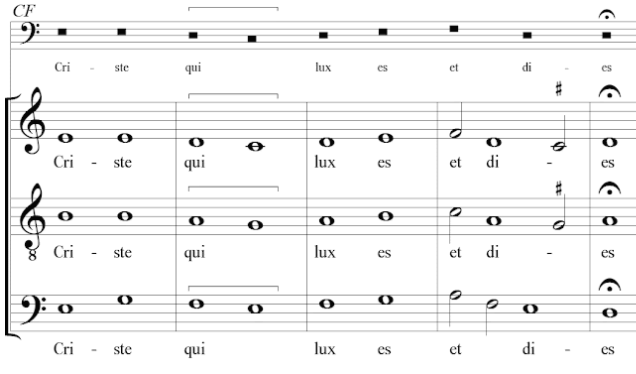
\includegraphics[width=.8\textwidth]{images/chapter1/fauxbourdon1.PNG}}
    %     \captionsetup{width=.5\textwidth}
    %     \caption[An excerpt demonstrating one \textit{fauxbourdon} harmonization variant over a fixed cantus firmus. Note rhythmic isochrony and predominantly fixed intervallic relationships between voices.]{An excerpt demonstrating one \textit{fauxbourdon} harmonization variant over a fixed cantus firmus. Note rhythmic isochrony and predominantly fixed intervallic relationships between voices.\footnotemark}
    %     \label{fig:fauxbourdon}
    % \end{figure}
    %     \footnotetext{\autocite[]{Rotem_2022}}

    % These universally stringent rhythmic and melodic ties to the cantus firmus rather strictly delimited the creative latitude afforded to any one practitioner. ``Improvisation'' such as it is in this context is token at best when compared with later, more sophisticated forms of truly polyphonic performance. As such, I consider \textit{fauxbourdon} less a fully-fledged open form and more a stylistic stepping-stone toward the sorts of open music practices which concern this research.

    In contrast with other (earlier and contemporary) literate musics, \textit{Cantare super librum} clearly required a more robust sense of a desired aesthetic for the final work insofar as each participant was required to heed principles of good taste in their use of rhythmic motifs, melodic structure, cadences, etc., in effect each creating an independent contrapuntal voice in real time.\footnote{
        To anticipate a potential objection: The practice of \textit{fauxbourdon} whereby, broadly, singers added parallel consonances in rhythmic isochrony to a cantus firmus similarly required both musical literacy and some degree of extemporization. These techniques were practiced concurrently with \textit{cantare super librum}, but also preceded its use in the church by centuries. As such, \textit{fauxbourdon} might fairly be considered a hinge-point in Western notation worthy of inclusion in this survey. However, while the precise intervallic relationship between cantus, tenor, and other voices differed geographically and by era, within a given \textit{fauxbourdon} tradition, these relationships were more or less static, only rarely departing from their stolid, homophonic note-against-note texture. (\autocite[434--7]{Taruskin_2009}) Thus, while there was no doubt some degree of extemporization (embellishments, cadences, etc.), \textit{fauxbourdon} rather strictly delimited the creative latitude afforded to any one practitioner. ``Improvisation'' such as it is in this context is token at best in contrast with later, more sophisticated forms of authentically polyphonic performance. As such, I consider \textit{fauxbourdon} less a fully-fledged open form and more a stylistic steppingstone toward the sorts of open music practices which concern this research.
    }
    As such, the practice also necessitated a greater ability to ``see through'' the open skeletal framework provided by notation into (what we'll dub) the ``field of musical potential'' --- i.e. the network of musical moves available to a performer which fulfill the demands of the work-concept as it is understood.

        \begin{figure}
            \centering
            \fbox{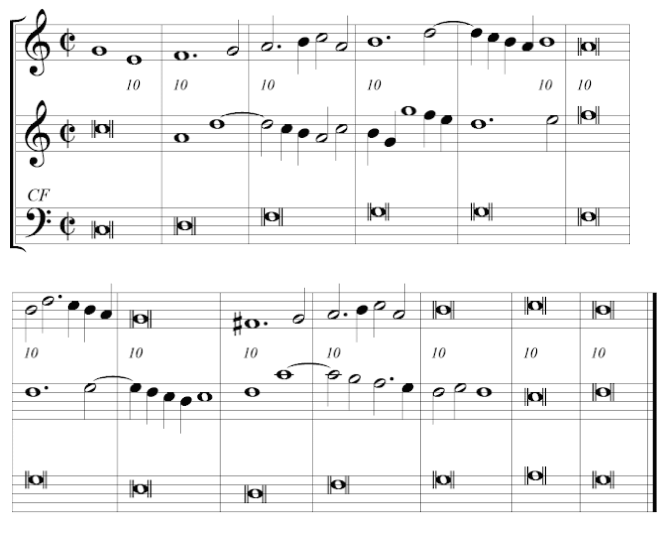
\includegraphics[width=.8\textwidth]{images/chapter1/cantaresuperlibrum1.png}}
            \captionsetup{width=.5\textwidth}
            \caption[A hypothetical contrapuntal ``illumination'' of a cantus firmus realized in a \textit{cantare super librum} style, per later sixteenth-century Italian pedagogical manuscripts.]{A hypothetical contrapuntal ``illumination'' of a cantus firmus realized in a \textit{cantare super librum} style, per instructions elucidated in later sixteenth-century Italian pedagogical manuscripts.\footnotemark}
            \label{fig:cantare}
        \end{figure}
            \footnotetext{\autocite[]{Rotem_2022}}

    Figure~\ref{fig:cantare} above is, of course, only a hypothetical example, helpfully constructed using contemporary sources by early music scholar Elam Rotem. Though presumably the occasional masterpiece extemporization was transcribed for posterity, as with all improvisatory practices the vast, vast majority of \textit{cantare} realizations have been lost to time. While methods varied greatly across Europe during the fifteenth century, certain techniques like the embellished ``parallel tenths'' model shown in the figure turn up frequently enough to be identified as a core improvisational strategy.\autocite{Rotem_2022} Pedagogical treatises, like those of Johannes Tinctoris and his descendants, can give the modern reader a sense of what it must have been like to engage with a cantus firmus \textit{qua} open notation. Universally, these manuals present the reader with potential contrapuntal embellishments---solutions to various intervallic scenarios which over time become familiar enough to the student that recognized patterns in liturgical melodies begin to afford these embellishments directly in performance. Figure~\ref{fig:lusitano} illustrates three such bite-sized affordances. In the first of these, a stepwise descent in the bass from D to C presents the possibility of a symmetrical stepwise ascent of a 7th in a particular rhythmic pattern. The second shows the inversion of the first, and the third demonstrates a more complex solution over a longer cantus segment. To the fifteenth-century improvising cantor, the aforementioned ``field of musical potential'' which avails itself \textit{via} the unadorned cantus firmus comprises a sort of networked map, itself comprising countless such embellishments, harmonizations or diminutions---first learned by rote then ``forgotten.''\footnote{(to borrow a turn of phrase perhaps apocryphally ascribed to Charlie Parker)}

        \begin{figure}
            \centering
            \fbox{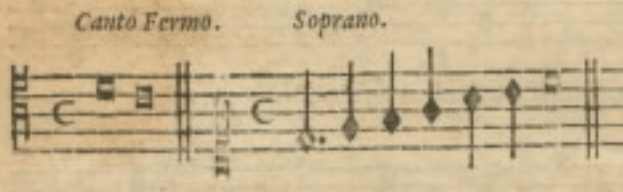
\includegraphics[width=.5\textwidth]
            {images/chapter1/lusitano1.png}}
            \fbox{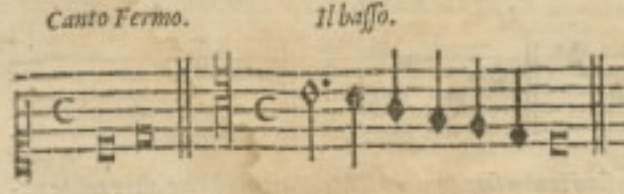
\includegraphics[width=.5\textwidth]{images/chapter1/lusitano2.png}}
            \fbox{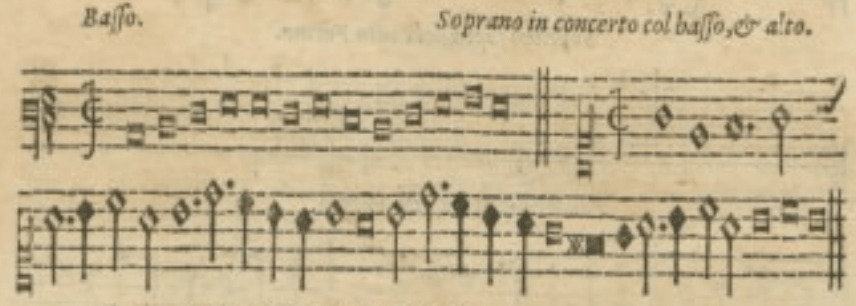
\includegraphics[width=.7\textwidth]{images/chapter1/lusitano4.png}}
            \captionsetup{width=.5\textwidth}
            \caption[Pedagogical ``sample'' realizations of short cantus firmi, from Vicente Lusitano's 1553 treatise \textit{Introduttione facilissima}.]{Pedagogical ``sample'' realizations of short cantus firmi, from Vicente Lusitano's 1553 treatise \textit{Introduttione facilissima}.\footnotemark}
            \label{fig:lusitano}
        \end{figure}
            \footnotetext{\autocite[15]{Lusitano_1561}.}

    It is my contention that the fundamental (``phenomenological,'' if you like) experience of the \textit{cantare super librum} improviser is, despite the vast historical gulf separating them, predominantly similar to the experience of later notation-mediated improvising musicians, be they continuo harpsichordists or bebop trumpet-players. In each case, a musician has the ability to ``acquire'' a skeletal compositional form via notation (one which, if rendered ``directly''---i.e. played note-for-note---would represent a hopelessly impoverished example of the work itself) which they are then expected to illuminate via a series of embellishments or wholesale inventions mediated by strictures communicated by the form itself. These written forms, of course, vary in the degree of detail they express; that is, in the closeness with which their symbolic systems correspond to the finished product (their \textit{fixity}). The performer here constantly negotiates between the printed material, their personal ``field of musical potential'' acquired via training and experience, their commitments to the performance scenario (e.g. ``Is this realization appropriate to this time/place/work?''), and, arguably, their sense of artistic identity (e.g. ``Does this realization adequately represent \textit{me} as an artist?'').

    Of course, each musician operating in these disparate genres bears a different, personal relationship to notation itself---indeed, there have been exemplary figures in every era who reach astounding levels of improvisational sensitivity despite being musically ``illiterate.'' Musician-to-musician and teacher-to-student o/aural transmission have, in all cases, formed a crucial component in the building of these ``fields'' of potential musical moves. To again cite Laurenz L\"utteken, ``[m]usic does not need to be fixed or transmitted in written form to constitute a work'' and neither must musicians necessarily engage with score-artifacts in order to take part in their associated literate traditions.\autocite{Lutteken_2020} However, contrary to all-too-prevalent attitudes that notation somehow ontologically lags behind music making proper, parasitically dependent on o/aurality for its very existence, I share Floris Schuiling's view that notations themselves ``serve to construct forms of musical interaction [...] offer[ing] different ways of imagining sound as music, make different demands on musical knowledge, and condition musicians' creative agency.''\autocite[431]{Schuiling_2019} As such, the notion that (western) music notation is inevitably downstream from somehow ``purer'' acts of music making is, in my view, untenable. When a notational practice (predominantly open or otherwise) is so inextricably integrated with the learning, dissemination, and reification of musical works, there is a very real sense in which even the musically ``illiterate'' still engage, by proxy, with structures of notation. 

    Even insofar as a musician might ``graduate'' from the printed page--- becoming so familiar with an oft-repeated work that s/he no longer needs to physically peer at its skeletal frame---s/he still renders the work in real time using sound-concepts that are best and most often expressed in the system of notation surrounding the work's associated corpus. To reiterate: I take it that this relationship between musician and notation (i.e. between artist/artisan and material) constitutes a style of notational mediation which permanently refigured the nature of (western art) music-making and which, in essence, still constitutes a large part of the experience of modern musicians today. 
    
    % \begin{notestuff}
    %     Per a comment from Amy, I think I'll reorganize this section a bit, adding in one or two contemporary sources (one or two figured bass manuals advocating for particular sorts of improvisatory performance) and relocate my commentary to a later section.
    % \end{notestuff} 

    In sum, the fifteenth century represents a crucial locus for the development of modern notational practices. First, it sees the rise of a mature mensural notation; one which records both absolute pitch and proportional durational values using a far more robust encoding scheme than in previous generations. Second, the way notation is used in the fifteenth century begins to resemble contemporary usage to a much greater extent in that it gains performative rather than strictly archival/pedagogical utility. The preponderance of theoretical treatises written during this period as well as the new flourishing of complex (written) works which approach composition from a ``notation-first'' perspective demonstrate that key aspects of the notion of literacy so central to Western art music today were in full swing over half a millennium ago.\footnote{See, for instance, Ockeghem's experimental \textit{Missa Prolationum} which arguably centers the \textit{manipulation of a symbolic system} as its main compositional process over and above merely crafting a beautiful, genre-appropriate sound-world.} 

    There is a very real sense in which fifteenth-century Western notation (particularly notation employed in expressly improvisatory genres like \textit{cantare super librum}) utterly relies on its openness. The notion that a piece of music could somehow be ``fully represented'' by its score or parts is fundamentally incompatible with the way written music was performed during this era---whether primarily improvised or merely ornamented. Much like the more recent examples of open/literate music-making to be described in later sections, the fifteenth-century musical work-concept only forms at the nexus of composer, performer, and score-artifact---a relationship mediated in no small part by the nature of the symbols themselves.
    
   % \begin{uselater}
   %     ...what remains is for composers to begin deploying purpose-built tools to wield + change the performer's improvisatory capabilities.
   % \end{uselater}

\section{Post-fifteenth-century reforms in open notation}
   
     %\paragraph{\textit{Basso continuo} and figured-bass}
     Above, I argued that the experiential kernel at the heart of open/literate music performance began, in essence, with improvisatory fifteenth-century polyphony. Of course, this is not to say that the intervening centuries between the fifteenth- and twenty-first did not see their share of important development in the art of open notation. Making its first documented appearance in the literature via a Roman manuscript in 1600, the practice of figured \textit{basso continuo}---likely far more familiar to modern readers than \textit{cantare super librum}---would become arguably the most prevalent and durable open notation in Western art music, representing one of the richest examples of a highly o/aural yet strongly notation-mediated performance practice in the literature.\autocite[811]{Taruskin_2009} Though, to be clear, this chapter lacks the space for any truly detailed treatment of the topic, it should suffice for future comparisons to briefly gloss its novel open notation scheme.

    In essence, \textit{basso continuo} refers to both (a) an inscribed bass line and concomitant harmonic structure which, together, undergird a (typically Baroque) performance and (b) the performance practice itself. While frequently used to notate accompanimental sub-ensembles, it crops up often in pieces for unaccompanied homophonic instruments (organ, lute, harpsichord, etc.). Given that \textit{basso continuo} flourished for over 150 years, the technique appeared with many variations according to local convention, though all share a composer-provided bassline (meant to be performed as-written with little variation) and some means of encoding operant harmonies over which the performer improvises according to certain constraints. Though in modern parlance the term is frequently interchanged with ``figured-bass,'' instrumental improvisation over basslines of the \textit{continuo} form long preceded the development of the accompanying numeric figurations. To be precise, Marla Hammel locates the origin of un-figured \textit{continuo} \textit{avant la lettre} in the aforementioned early polyphonic music of the Catholic church. Figured-bass proper, on the other hand, began in Rome and quickly spread outward owing to its many advantages over the more opaque un-figured variety.\autocite[28--9]{Hammel_1977}

    Jeffery Kite-Powell elaborates in his \textit{Performer's Guide to Seventeenth-Century Music}: 

        \begin{smallquote}
            The idea of adding a chordal accompaniment to vocal or instrumental pieces had been practiced in one way or another for over a century, either by improvisation or by reading ``short score'' [...] but the practice grew with special intensity in the declining years of the sixteenth century as musicians began writing---and publishing---such music in the convenient method of figured (and unfigured) basses. As the practice spread, it was applied to older-style polyphonic textures, as well as to the newer ones of solo melody.\autocite[317]{Kite-Powell_2012}
        \end{smallquote}

    This ``shorthand'' most often takes the form of numeric figuration beneath the given bassline (of the form $^{5}_{3}$, $^{4}_{2}$, $^{\sharp6}$, etc.) which, at a minimum, indicates to a performer which intervals are to be sounded above the bassline---usually without reference to a particular octave. More than mere stand-ins for un-notated tones, though, these numeric glyphs imply particular harmonic fields which in turn form the basis of the performer's improvisatory embellishments on the fundamental line. Figure~\ref{fig:figuredbass} gives a paradigmatic example of figured bass notation as used in Georg Philipp Telemann's violin sonata, TWV 41:F3 (1734) illustrating the soloist's melody with figured bass beneath.
    
      \begin{figure}
            \centering
            \fbox{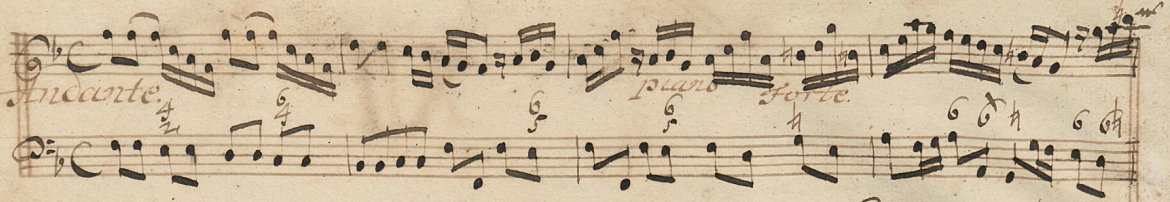
\includegraphics[width=.9\textwidth]{images/chapter1/telemann1.png}}
            \captionsetup{width=.5\textwidth}
            \caption[A paradigmatic sample of figured bass notation from Telemann's violin sonata TWV 41:F3. Drawn from a contemporary manuscript.]{A paradigmatic sample of figured bass notation from Telemann's violin sonata TWV 41:F3. Drawn from a contemporary manuscript.\footnotemark}
            \label{fig:figuredbass}
        \end{figure}
            \footnotetext{\fullcite[]{Telemann_1734}}

    To appropriately realize a figured-bass passage is to delicately balance \textit{recitation}, i.e., recreating the specified bassline and intervals above, and \textit{creation}, i.e., ``seeing through'' the simple figures to the implied harmonic function and reinforcing it through improvisation. Of course, this raises new questions: If earlier, un-figured lines were sufficient to improvise ``over the book'' or to provide accompaniment to a soloist, then why was it necessary to conceive and deploy an entirely new set of glyphs---i.e. yet another system to teach and to memorize? And what significance do these new symbols have to the relationship between performer and score if performers were getting on well enough without them? 
    
    In essence, figured \textit{continuo} was a labor-saving device; a novel musico-graphic technology. The skills required to quickly examine a number of vocal or instrumental parts (or even a lone bassline) and extract enough salient harmonic information to cogently improvise behind an ensemble required extensive training: time and money. These figurations allowed a composer to much more efficiently and precisely communicate a piece's harmonic structure to a would-be improviser while also allowing less-musically-literate performers the opportunity to meaningfully participate in otherwise inaccessible music. Though the degree of figuration provided would differ according to time, place, composer, and publisher, to the extent that they were present these figures lent performers more clarity and composers greater control of the otherwise thorny, opaque process of improvisational accompaniment.\autocite[321]{Kite-Powell_2012}

    Ultimately, I contend that \textit{basso continuo} still fundamentally upholds the \textit{cantare} model of composition/improvisation insofar as it is still ultimately left up to the performers' training and good taste to determine the authentic/appropriate bounds for their contributions. However, the introduction of a new, bespoke system for encoding harmonic information does represent an important turning point in Western notation. Specifically, it marks an early concerted effort to sculpt and/or facilitate the communication of the boundaries of improvisatory musicmaking. Musical glyphs had, since the fifteenth century at latest, been forced to pull double-duty in somehow representing not only the fixed parameters of performance but the open ones as well. Though figurations would never fully obviate performer expertise in sussing out these open parameters, they provided a simple graphic synopsis through which to conceptualize a work's changing harmonic field (and indeed even even harmony generally).
    
    %        \begin{uselater}
    %            Two more paragraphs here explaining how figured bass is the result of economic/sociological pressures---how they are coded communication from the composer to the performer that they're expected to improvise under constraints---that they represent a new VERTICAL conception of harmony---how I'll touch later on 20th-century chord symbols (and that they're basically the same thing) and that they're really interesting but I don't have the space. I should probably cite a pedagogical treatise which mentions the sorts of creative liberties afforded to the performer! Then do my little finishing paragraph at the end of the section. 
    %            
    %            In short, it grants composers more precision in sculpting their performers' improvisatory efforts; it facilitates pedagogy rather than hindering it; it allows the dissemination of musical materials to newly-literate groups of musicians. 
    %        
    %            Why is this relevant to narrative? Well, it's a concrete piece of notational technology invented to facilitate communication of the boundaries of improvisation.
    %        \end{uselater}
        
    
    %    A more detailed treatment of this topic would, no doubt, delve further into the increasing sophistication with which composers (for a variety of reasons) begin to incorporate open materials into their works in the ensuing centuries. First ``officially'' entering the literature via a Roman manuscript in 1600, the practice of \textit{basso continuo}---arguably the arch-open-notation in terms of its relative prevalence and durability---represents one of the richest examples of a strongly o/aural yet equally notation-mediated performance practice in the literature.\autocite[811]{Taruskin_2009} Further, its use of both a skeletal melody \textit{and} an associated ``vertical'' conception of harmony (new for the seventeeth century!) cements it as the tradition which bears the strongest resemblance to today's lead-sheet-mediated jazz performance, perhaps our most universally familiar literate open music practice. Figure~\ref{fig:figuredbass} gives a paradigmatic example of figured bass notation belonging to Telemann's TWV 41:F3. 

    As any student of music history is aware, though, this long, rich period of well-integrated literate/improvisatory practice was not to last forever. Certainly, the bulk of Western art music practiced today demonstrates a far scantier degree of interpretive latitude when it comes to score-reading. Robin Moore, in an essay titled ``The Decline of Improvisation in Western Art Music,'' sums up: Today, he claims, ``[t]he mandates of compositionally specified interpretation now supersede those of the instrumentalist. To many, improvisatory expression seems threatening, unfamiliar, or undeserving of interest.''\autocite[63]{Moore_1992} 
    
    Of course, despite the fact that the musical period marked by widespread \textit{continuo} practice is commonly thought of as the local apex of ``classical'' improvisation, this is not to suggest that improvisation in Western art music surreptitiously vanished at the end of the Baroque period. Eighteenth-century giants W. A. Mozart and Ludwig Beethoven are generally noted to have been skilled improvisers whose extemporizations often made their way into their finished works. Indeed, as Moore continues,

        \begin{smallquote}
            Even well into the 19th century it is clear that improvisation remained an indispensable ability for most professional musicians. We know that Brahms, Paganini, Chopin, Clara and Robert Schumann, Mendelssohn, Hummel, Cramer, Ries, Spohr, Joachim, and Schubert, to cite a few familiar names, were all accomplished improvisers in addition to composers and/or performers of precomposed music.
        \end{smallquote}
    
    \noindent Further, systematized improvisatory styles waxed and waned in intervening centuries. French liturgical organ music, for instance, saw increasingly codified improvisation throughout the eighteenth and nineteenth centuries, expounded upon by contemporary scholar-pedagogues like Alexandre-Étienne Choron\footnote{\textit{Sommaire de l'Histoire de la Musique} (1810)}, François-Joseph Fétis\footnote{\textit{Méthode élémentaire de plain-chant à l'usage des séminaires, des chantres et organistes} (1843)}, and their heirs Louis Niedermeyer and Joseph d'Ortigue\footnote{\textit{Gregorian Accompaniment: A Theoretical and Practical Treatise Upon the Accompaniment of Plainsong} (1856--7) (helpfully available in English, translated by Wallace Goodrich)}, François-Auguste Gevaert\footnote{\textit{Méthode pour l'Enseignement du Plain-chant et la Manière de l'Accompagner, Suivie de Nombreux Exemples} (1856)}, and Jacques-Nicolas Lemmens.\footnote{\textit{Du Chant Gregorien, sa Melodie, son Rythme, son Harmonisation} (1886 posth.)}

    These improvisatory practices, however, differ from those of the Baroque and Renaissance in one critical sense. Rather than make use of yet more sophisticated notations-for-improvisers, they instead (in a sense) retrogress. As the eighteenth century wears on, music begins to become more and more fixed-in-place on the score: where improvisation occurs, it occurs \textit{contra} the score rather than through it. The next section of this chapter will briefly attempt to account for this historical waning of open-notation-centric performance models and the turn toward yet greater degrees of notational fixity in the late-eighteenth and nineteenth centuries.

        %\begin{uselater}
        %    Argue that FB was basically the apex of open/literate music but concede that it wasn't totally static. Maybe this couple of paragraphs could just be merged into the next section.
        %\end{uselater}
        %
        %    \begin{notestuff}
        %        I should rephrase the following paragraph. Concede that things did change but that for the purposes of our larger-scale ``ebb-and-flow'' narrative, the most significant changes in Western music notation came with the concretization of the work-concept during the galant. It's what I'm going into in the next section, so I just need to signpost that discussion.
        %    
        %        Something like:
        %    
        %        While further discussion of these smaller-scale developments in Western notation-mediation is long overdue, the space allotted here is unfortunately insufficient to do any serious work here. On the larger scale...
        %    \end{notestuff}
   
    %    \paragraph{Other open/literate musics} Especially in France, various styles of improvisation at the organ, too, developed in intervening centuries. These are expounded upon in treatises by eighteenth- and nineteenth-century writers such as Alexandre-Étienne Choron\footnote{\textit{Sommaire de l'Histoire de la Musique} (1810)}, François-Joseph Fétis\footnote{\textit{Méthode élémentaire de plain-chant à l'usage des séminaires, des chantres et organistes} (1843)}, and their heirs Louis Niedermeyer and Joseph d'Ortigue\footnote{\textit{Gregorian Accompaniment: A Theoretical and Practical Treatise Upon the Accompaniment of Plainsong} (1856--7) (helpfully available in English, translated by Wallace Goodrich)}, François-Auguste Gevaert\footnote{\textit{Méthode pour l'Enseignement du Plain-chant et la Manière de l'Accompagner, Suivie de Nombreux Exemples} (1856)}, and Jacques-Nicolas Lemmens.\footnote{\textit{Du Chant Gregorien, sa Melodie, son Rythme, son Harmonisation} (1886 posth.)} These methods of plainchant accompaniment, though distinct, likewise involve a similar ``deep'' literacy as regards the illumination of sparse, open printed materials---which may take simpler forms (adding isochronous, vertical harmonizations below a chant, for example) or more complex ones (full, multi-voice counterpoint which sequesters the original chant somewhere in an inner voice).

    %Bracketing further discussion of these and other fascinating examples of the flourishing of open notation, it must suffice for now to stake out the claim that (insofar as said notation is concerned), players' overarching musical roles underwent no massive paradigm shift between the mid-fifteenth century and, say, the galant period ending in the late eighteenth century. It is clear, though, that \textit{unlike} practices of literate improvisation or other creative musical interpretation during this long historical era, Western art music as practiced today (barring post-1970 changes which we'll discuss presently) features a far scantier degree of interpretive latitude when it comes to reading music. Per Robin Moore, ``The mandates of compositionally specified interpretation now supersede those of the instrumentalist. To many, improvisatory expression seems threatening, unfamiliar, or undeserving of interest.''\autocite[63]{Moore_1992} The next section of this chapter will briefly attempt to account for this historical waning of open-score-centric performance models and the turn toward yet greater degrees of notational fixity in the late-eighteenth and nineteenth centuries.
        
        %%%%%%%%%%%%%%%%%%%%%%%%%%%%%%%%%%%
        %%% LITTLE ORPHANED TOPICS %%%%%%%%
        %%%%%%%%%%%%%%%%%%%%%%%%%%%%%%%%%%%
        
        %It is clear, though, that \textit{unlike} the dominant art music paradigm with which we entered the twentieth century, that of the fifteenth century also demanded a different sort of literacy: namely, a well-developed relationship to open scores and familiarity with the processes by which they were to be brought to completion in performance. BIG CHANGES IN WHAT CONSTITUTES LITERACY
        
        %However, he is quick to point out that as of the fifteenth century, ``[n]otated compositions were treated as `works' in that they record[ed] how the music existed in performance, not insofar as they serve[d] as a prescriptive prompt for future presentation: the `work quality' inhered in the performance itself, not the written memento.''
        
        %\textcolor{red}{[of course, making positive claims about how music's openness was perceived/utilized at the time of its creation is nigh impossible -- but turning to contemporary performance guides can give us insight into the sorts of affordances notation carried with it. What sort of fields of sonic/action potential ]}
        
        %\textcolor{red}{
        %[The development of the work-concept in the fifteenth C.]
        %[Cantare Super Librum -- taruskin p.436-438]
        %[Prelude to figured bass -- structured improvisation based on a single melodic line]
        %[Diminutions as score-oriented improvisatory practice]
        %[First printed continuo -- taruskin p.811]
        %}
        
        %    \section{Openess in the common-practice period}
        %\textcolor{red}{
        %    [MAYBE CUT THIS SECTION ENTIRELY --  I THINK OPEN NOTATION EXPERIENCES ARE SIMILAR ENOUGH BETWEEN END OF RENAISSANCE AND COMMON-PRACTICE THAT WE COULD GO RIGHT TO ROMANTIC CONCRETIZATION]
        %    [Maturation of continuo practice -- resembling lead-sheets... but also the beginning of the end?] 
        %    }

    \section{Concretizing the sound-concept}
        
        % \begin{notestuff}
        % \begin{itemize}
        %     %\item \textcolor{red}{[Goal here is 99\% well-cited historical account and 1\% commentary.]}
            
        %      % \item Throughout this paper I have perhaps somewhat carelessly conflated ``improvisation'' (a term both extremely vague and hopelessly loaded) with the realization of notation of \textit{any} degree of openness. This is on purpose. I see no difference-in-kind between a long extemporization on a D-dorian chord/scale in the context of a jazz tune and the trivial decision to interpret a melodic fragment \textit{molto secco} rather than \textit{espressivo}... This might need some explanation though?? --- The rise of notational fixity == the closing off of the ``field of musical potential'' == more semantic content packed into each unit of notation
        
        %     %\item \textcolor{red}{Hammel cites ``the demise of partimento in Italy'' as a transition away from improvisation practices}
        
        %     %\item \textcolor{red}{There should be some attempt to track actual changes in the glyphs. Additions of more and more detailed dynamic markings, hairpins, etc., as well as articulations and expressive texts and specific tempo markings. --- Not to mention the decline of abbreviated embellishments (turn, mordant, etc)}
        
        %     %\item Beethoven's early works serve as another important hinge-point in their omission of the embellishments that characterized the prior 200 years or so...
        
        %     %\item Beethoven, of course, adds turns and trills into his music but these now serve more as a composer's shorthand---a notational device used to save ink rather than to inject a measure of improvisational spontaneity and freshness into an otherwise unchanging score.
        
        %     % \item ``...unwritten ornaments were still routinely employed and expected in Italian recitative as late as the 1850s, whereas many performers beginning in the 1880s took to `weeding them out' even in Mozart, reflecting a new literalism that affected the way in which notation was interpreted as soon as unwritten (`oral') traditions lost their sway in pedagogy. What was mistakenly viewed as the removal of inauthentic accretions was in fact a modernization.\autocite[591]{Taruskin_2009a}''\
        
        %     %\item ``In 1852, Johann Georg Meister made the sober assessment that `[h]armony and thoroughbass are therefore fairly equivalent in their meaning.\footcite[6]{Diergarten_2011}'
        
        %     %\item Certainly seems like some combination of more musicians = less time per musician to teach delicate improvisatory arts (teaching to read is far easier) + the adoption of German theoretical models in pedagogy over literate-improvisatory Italian partimento tradition...
        
        %     %\item (It's not only that notation simply took on a \textit{greater} role in music pedagogy/transmission, it's that notation was necessarily reduced to its simplest form---as representations of fixed aspects of a sound world.)
        % \end{itemize}
        % \end{notestuff}

    In a sense, a synopsis of the Romantic period could begin and end with George Lewis' terse assessment of the situation:

    \begin{smallquote}
        By the end of the nineteenth century, the practice of improvisation as a form of professionalized artmaking had all but disappeared from Western classical music. This gradual elimination of improvisation did not take place without resistance, most prominently including French organ performance. However, this break with what had heretofore been ``the'' Western tradition certainly constituted a radical rupture with over a half-millenium [sic] of canonical practice [...]\autocite{Lewis_2007}
    \end{smallquote}

    %\noindent However, for the purposes of our specifically notation-oriented narrative here, I take it that the topic deserves at least a little qualification. 
    Lewis' short paper (focusing primarily on recent developments in improvisation pedagogy) does not attempt to account for this decline, though a number of other authors have. Charles Rosen, in a paper on the role of ornamental gesture in Beethoven's corpus, describes the late-eighteenth-century decline of ``open'' ornamentation (e.g. appoggiaturas, trills, mordents, grace notes, passing tones, etc.; either deliberately written into the score at key points or generally understood to be permitted/desired) as ``one of history's most sweeping revolutions in taste.'' For Rosen, this was but one symptom of a culture-wide trend toward elegant simplicity and away from obscurant decoration: one which held sway in architecture and the fine arts just as much as it did in music. Whether the addition of improvised ornaments to Mozart's music constitutes an ``authentic'' eighteenth century practice remains a hotly contested issue. However, it seems to be a foregone conclusion that during the era of Beethoven's flourishing these additions were considered very much passé---even to the point that Carl Czerny drew the composer's ire when he, by second-nature, added trills and octave doublings to Beethoven's work.\autocite[1198--9]{Rosen_1970} This is to say nothing of the venerable practice of basso continuo which, per Taruskin, fell out of general favor during the mid eighteenth-century\autocite[428]{Taruskin_2009a} and suffered a fatal blow via its omission from Christoph Gluck's opera \textit{Orfeo ed Euridice} (1762)---``the first opera that [could] be performed without the use of any continuo-realizing instruments''.\autocite[457]{Taruskin_2009b}

    In broad strokes, these changes in the function of notation whether visible (in the case of the disappearing continuo) or invisible (the proscription of the traditional ``un-notated'' embellishments) pointed to a radically transfigured art music landscape---one in the process of transferring creative agency away from performers and toward composers who, increasingly, bore the responsibility of fixing \textit{one} particular sonic realization of a work into notation: a realization wholly imagined by the composer him/herself. The sonic traces of the old embellishments persisted, of course. While penning his violin sonatas Beethoven imagined and recorded the same trills, turns, and keyboard harmonies to which he had grown accustomed over the course of his musical upbringing---no doubt improvised in many cases by diligent performers. The critical difference is that by the late eighteenth/early nineteenth century, Beethoven and his contemporaries began \textit{concretizing} these same gestures; in effect rendering their received notational tools more semantically fixed than ever before. Thus while the casual listener, unfamiliar with this radical new \textit{fixing} of notation semantics, would not necessarily notice a change insofar as the sound/gesture is concerned, the nineteenth-century performer accustomed to a distinctly open mode of play now bears an entirely new relationship to the score-artifact: one characterized far more by mechanical reproduction that by artisanal creation. Figure~\ref{fig:beethoven} gives a token example taken from the famous \textit{Kreuzer Sonata} illustrating a typical deployment of Beethoven's embellishments. A century prior, a violinist approaching this passage would have had a plethora of interpretive possibilities open to him given the extent to which his practice was necessarily embedded in open notation. Beethoven's violinist, on the other hand, is condemned to read \textbf{\textit{tr}} in a very particular way; conditioned by decades of pedagogical texts which were more strict in their gestural prescriptions. In other words, the eighteenth-century \textbf{\textit{tr}} grants far less creative latitude than the seventeenth-century equivalent despite comprising the very same symbol.
    
    % A century earlier, a violinist approaching this passage sans (having been brought up in a tradition entirely dependent on open notation) would have a plethora of interpretive possibilities open to him. Beethoven's violinist, however, despite gazing at the \textit{same symbols} now has much less latitude when it comes to precisely how the D$\sharp$ in measure 75 will resolve to the E in measure 76. 
    
    % \begin{notestuff}
    %     Michael wants me to clarify the previous sentence.
    % \end{notestuff}
    
        \begin{figure}
            \centering
            \fbox{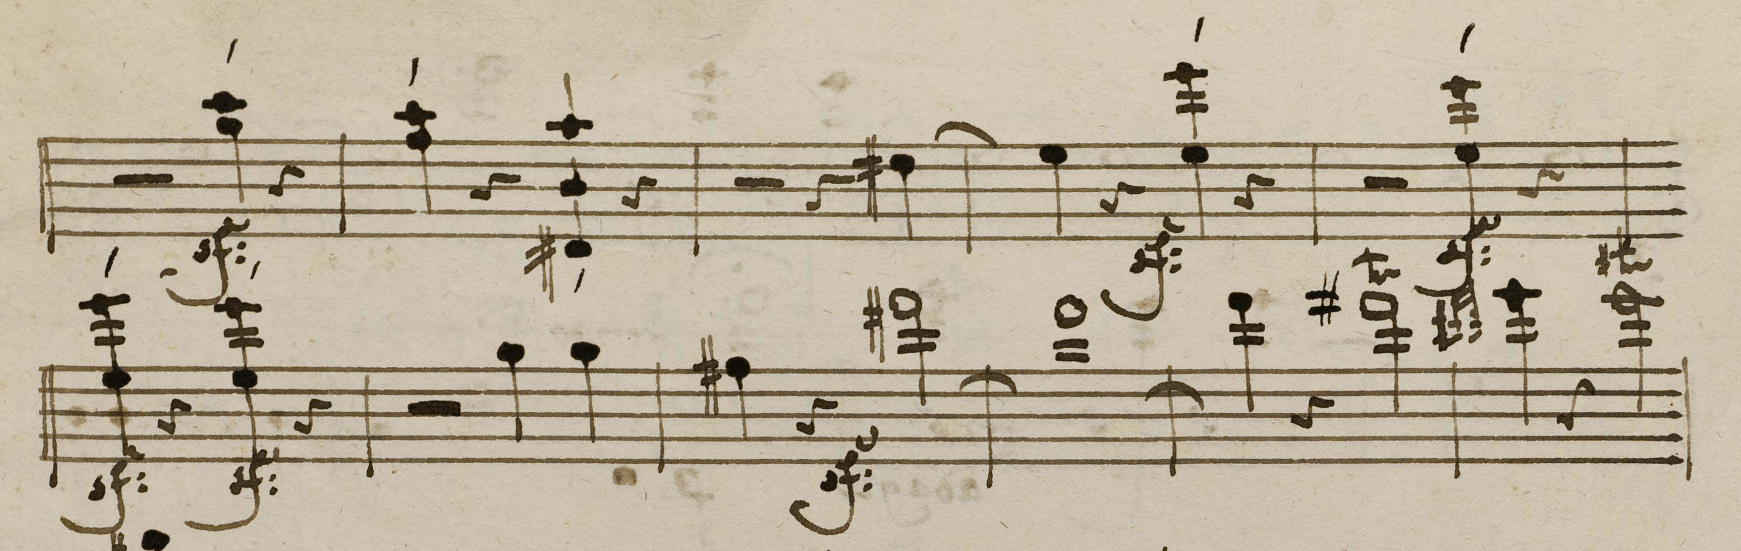
\includegraphics[width=.9\textwidth]{images/chapter1/beethoven_kreuzer_mm66-76.png}}
            \captionsetup{width=.5\textwidth}
            \caption[Mm. 66--76 from Beethoven's \textit{Kreuzer Sonata}. Violin part excerpted from original manuscript.]{Mm. 66--76 from Beethoven's \textit{Kreuzer Sonata}. Violin part excerpted from original manuscript.\footnotemark}
            \label{fig:beethoven}
        \end{figure}
            \footnotetext{\fullcite[]{Beethoven_manuscript}}

    To sum up, two major changes in the printed page have taken place: first, the glyphs which explicitly grant improvisatory latitude to the performer---namely, figured bass indications and the host of baroque ornamentation symbols---have been stripped away, replaced by precise voicings and occasional \textbf{\textit{tr}} markings. Second, beyond the addition of fully-realized harmonies which replace the now-missing figured bass, composers began delineating their idealized performance further still via the use of more frequent and more specific dynamic indications, tempo markings, articulations and expressive text. This is of course not to claim that broader improvisational practices disappeared all together during this period---Beethoven, like the vast majority of his professional peers, was known to have been a talented improviser.\autocite[652--3]{Taruskin_2009b} Further, his explicit instruction in the ``Emperor'' concerto to ``not make a cadenza here, but play immediately the following [...]'' illustrates that performers were still commonly expected to freely improvise at cadences at least as late as 1809---though it gradually became more commonplace over the nineteenth century to merely execute fully-notated composer-provided cadenzas.\autocite[45]{Swain_1988} Thus, perhaps predictably, it seems that the first casualty of the large-scale trend toward the fixity of the sound-concept (which will eventually result in the disappearance of nearly \textit{all} Western art music improvisation by the turn of the twentieth century) is the notation which traditionally represented its \textit{openness}.
    
    Accounts of this decline in performer agency seem, broadly, to take two different tacks; centering either changes in \textit{aesthetic values} over the long eighteenth century or changes in \textit{socioeconomic factors}. Where Charles Rosen cites a ``solid body of aesthetic doctrine which condemned ornament [considered whole] as immoral,''\autocite[1198]{Rosen_1970} Robin Moore's more detailed essay considers aesthetics to be functionally downstream of ``the effect of technological development and industrialization,'' as well as ``the effect[s] of notation and literacy.''\autocite[80]{Moore_1992} Felix Diergarten further expounds on these pedagogical causes by describing an invisible war which took place in nineteenth-century music academies between proponents of the agèd Italian partimento tradition and those of the new German models of music theory.\autocite{Diergarten_2011} Partimento pedagogy held that the most effective means of internalizing realities of musical composition and performance was its practice. Students were exposed early on to countless musical prototypes and exemplars, perhaps the most famous of which was the \textit{regola dell'ottava}---the rule of the octave---which served as a schema by which a student could harmonize arbitrarily complex basslines \textit{ex tempore}. Only via this vocabulary-focused hands-on approach did students gain insight into what motivated particular ``musical moves'' compositionally and, in tandem, learn to build this vocabulary into their personal, improvisatory, network of musical moves. The German approach, on the other hand, eschewed these ``recipes and household remedies'' in favor of logically organized principles: universally applicable rules able to explain in hierarchical terms what motivated movement from tonic to dominant or why some tones seemed to supervene on others\autocite[9]{Diergarten_2011}. Though these two approaches persisted contemporaneously for some time, it was ultimately the latter system which won out---as might be demonstrated by peering at any undergraduate theory syllabus written in the past hundred years or so.

    Robin Moore buttresses this socioeconomic/pedagogical argument and specifically tethers the decline of improvisatory practice to (among many other factors) issues of notation. Per his 1992 paper ``The Decline of Improvisation in Western Art Music'',\footnote{Emphasis in quotes will be mine unless otherwise noted.}

        \begin{smallquote}
            The increasing importance of notation as a pedagogical tool and performance aid in the nineteenth century can similarly be explained in terms of the gradual replacement of the patronage musician at that time with the middle class performer. Scores and written arrangements for the piano were imperative to the dissemination of elite music among a broader audience in two senses. First they allowed for individual family members to learn music themselves, and to avoid the prohibitive costs of hiring professional musicians. [...] Secondly, \textit{notated music provided the detailed performative instructions necessary for those interested in learning to play a style of music with which they were unfamiliar. Sheet music became a means of learning aristocratic music for those who had no exposure to it in its original context.\autocite[72]{Moore_1992}}
        \end{smallquote}

    Here, I think, lies the simple math at the crux of the issue: once a more rarefied ecclesiastical (and/or) scholarly (and/or) aristocratic pursuit, art music had the luxury of a much smaller pedagogue-to-pupil ratio. As such, the tools of its creation and dissemination could be put to much subtler use. Students who had the privilege of close master/apprentice-style tutelage were able to develop literate improvisation schemas which corresponded closely to marks printed on the page. With the explosion of middle class performers (and performance opportunities), musicians had neither the time nor the money to dedicate years to the development of these schemas. Figure~\ref{fig:Corri} illustrates one of the first examples of music published for this growing market ``in »complete« form, with all necessary ornamentation written out in an appropriate manner for those who might otherwise be unable to interpret the score improvisationally."\autocite[72]{Moore_1992} Put simply, new, more ``fixed'' notation conventions (the standard trill in m. 11 and the turn and trill-to-mordant in m. 12) have replaced prior open notations and thereby obviated any knowledge of the delicate art of embellishment.

        \begin{figure}
            \centering
            \fbox{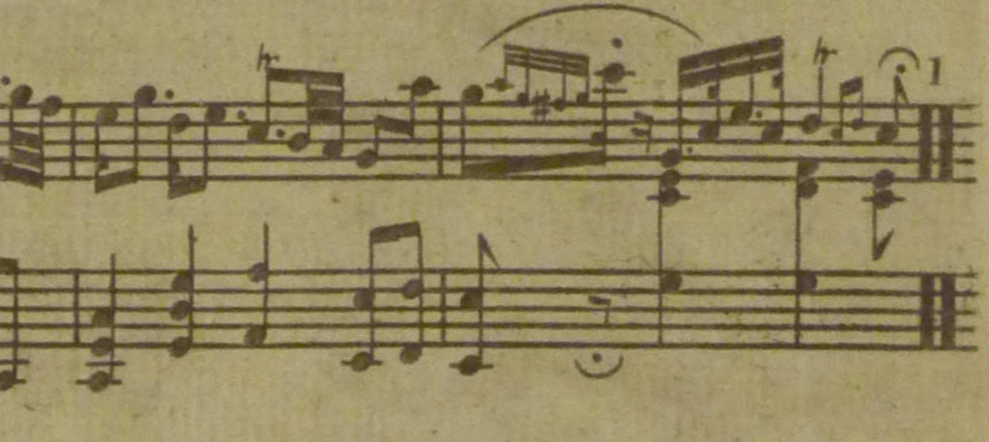
\includegraphics[width=.7\textwidth]{images/chapter1/corri1.png}}
            \captionsetup{width=.5\textwidth}
            \caption[Mm. 11--12 from the first Andante of Domenico Corri's breezy \textit{Loch Erroch Side} Variations demonstrating a carefully-realized cadence---far more ``fixed'' than earlier published keyboard works.]{Mm. 11--12 from the first Andante of Domenico Corri's \textit{Loch Erroch Side} Variations demonstrating a carefully-realized cadence---far more ``fixed'' than earlier published keyboard works.\footnotemark}
            \label{fig:Corri}
        \end{figure}
            \footnotetext{\autocite[]{Corri}}
    
    What was once merely the skeletal framework for a ``finished'' composition necessarily became representative of the entire sonic trace of the work---a condition which was, I take it, inextricable from a concomitant change in taste which demanded that the composer be responsible for the ``entirety'' of the work. Consequently, conservatories and other formal pedagogical centers either willingly or reluctantly began orienting their lessons toward this new fixed model of composition: to oversimplify, it seems that the explanatory power of German theoretical models benefited by having fixed pieces for analysis---complete at time of writing---rather than the more nebulous pre-nineteenth-century works which necessarily varied from performance to performance, relying on performers' input to ever be truly ``finished.''

    By the turn of the twentieth century, this new paradigm of notational fixity was thoroughly entrenched. While pockets of resistance clung tenaciously to life (e.g. in the aforementioned French liturgical tradition), Western art music notation by and large only developed insofar as it fixed the sound-concept of the musical work in finer and finer detail.\footnote{
        Consider, for instance, the growing compass of dynamic indications. Where, for Mozart (1756--91), a range of $\lilyDynamics{pp}$ to $\lilyDynamics{ff}$ was plenty (and these extremes only appear rarely), Tchaikovsky's (1840--93) oeuvre ranged from $\lilyDynamics{pppppp}$ to $\lilyDynamics{ffff}$ in his \textit{Pathétique} and Fifth Symphonies, respectively. Not to be outdone, György Ligeti's (1923--2006) range encompasses $\lilyDynamics{pppppppp}$ (Piano Étude No. 9) to $\lilyDynamics{ffffffffff}$ (\textit{Le Grand Macabre}).
        } 
    To this day, there is a very real sense in which art music in the European tradition is still produced and consumed under the hegemony of this nineteenth-century notation paradigm. To the extent that alternatives exist, they are practiced in the broad historical shadow of western notation---either derived from it (as is the case with the notation commonly used to record and study the Iranian \textit{radif} tradition---if not to teach it) or carved away as a ``subaltern'' which will necessarily be contrasted with it (as is the case with, for example, the various types of Japanese shakuhachi notation). Thanks in no small part to centuries of brutal colonial dominance by a ``global north'' whose modes of musical production often eclipse even long-lived local practices, western notation serves as a \textit{lingua franca} across (not all, but) a broad range of the world's musical styles and practices---both those which might fit under the umbrella of ``art music'' generally, as well as more quotidian vernacular practices. 

    In the next section, I'll discuss in brief the rise of perhaps the most successful challenge to this ``fixed paradigm''---the ascension of notation-mediated jazz improvisation---which coincided with jazz's own ascent from a rather localized vernacular music to a radically transfigured art music all its own. Given that this chapter has thus far served as a gloss of Western art music notation practices, this detour into a discussion of jazz notation might seem tangential. Our ultimate aim here, though, is a cogent analysis of a variety of specific open notation practices in the late twentieth century---many of which sit at the interstices between Western art music and jazz proper. Further, while most would not consider jazz (even in its mature form) to be an offshoot of Western art music \textit{per se}, the two have been, since the latter genre's nascence, hopelessly entwined---sharing mutual creative influence, personnel, theory, technique, and of course notation.
    

    \section[The Afro-diasporic return to open notation]{The Afro-diasporic return to open notation}

    To be crystal-clear up front: Jazz does not bear the same relationship to musical literacy as does western concert music. ``Literacy'' in the sense we have discussed it thus far is simply not a prerequisite for meaningful musical interaction in jazz performance. Paul Berliner's \textit{Thinking in Jazz} (1994), one of the most thorough jazz ethnographies published so far, cites several examples of renowned artists who attained fluency with western notation only quite late in their careers---and indeed stresses that in some cases an over-reliance on printed materials can meaningfully hinder jazz students' development\autocite[111]{Berliner_1994}. We might attribute this to the fact that jazz developed under radically different conditions than did western ``classical'' music. Autodidacticism and musician-to-musician o/aurality (to contrast with the centralized authority of the academy/conservatory and teacher-to-pupil o/aurality) traditionally played a much greater role in jazz than in the European tradition. In instances where students lacked the central knowledge base a formal institution which might favor transmission-by-notation, burgeoning jazz musicians might turn to direct transcription from recordings or other performances to acquire their improvisation schema and library of works. Further, many jazz instructors (despite a full working knowledge of western notation) deliberately de-emphasize(d) reading in their pedagogical practice---instead emphasizing the roles of listening and memory in acquiring and deploying genre-appropriate vocabulary.\autocite[112--3]{Berliner_1994} Debates over the relative worth of orality and literacy in jazz have been hashed out far better than I could hope to achieve here by the likes of Ingrid Monson, Gunther Schuller, and Berliner himself---thus I will stop short of throwing in my two cents on the topic. However, even if we admit to the notion that (as many would perhaps rightly claim) jazz is first and foremost an o/aural tradition, this fact does not preclude our consideration of the pivotal role that notation plays in its (again) pedagogy, acquisition and performance. 

    It is important to note that jazz was ``open'' before it was ever notated. To the extent that jazz performers have adopted techniques of western notation, they have always done so to further the agenda of open, largely improvised performance. That is to say: the primary mode of play in jazz performance centers on highly variegated renditions of existing tunes drawn from any number of creative wellsprings: original compositions, popular songs, folk tunes, etc. How far these renditions depart from some central, organizing artifact (be it one ``ancestral'' recorded performance, one particular arrangement, etc.) also varies from period to period and from sub-genre to sub-genre. While indeed the ``same-but-different'' model adopted by jazz performers bears a strong resemblance to aspects of figured-bass-oriented baroque performance practice, jazz renditions are often strikingly distinct (rhythmically, melodically, harmonically) from their original sources when compared to what we know of Renaissance and baroque improvisation. Figures~\ref{fig:MyFunnyOrig} and~\ref{fig:MyFunnyDavis} illustrate a particularly wide gap between original source and jazz rendition (a gap that forms an important part of Robert Walser's thesis in his fascinating 1993 paper ``Out of Notes'').

        \begin{figure}
            \centering
            \fbox{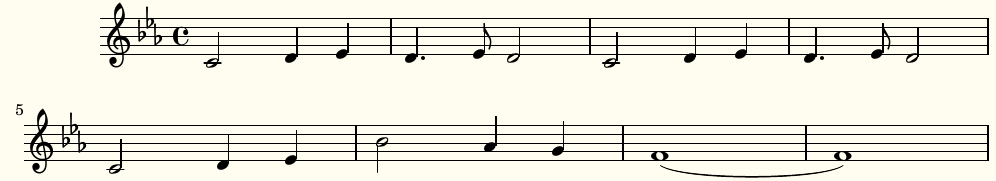
\includegraphics[width=.9\textwidth]{images/chapter1/davis_valentine2.png}}
            \captionsetup{width=.5\textwidth}
            \caption[First eight measures of the chorus to ``My Funny Valentine'' as originally printed in the 1937 edition (virtually identical to countless versions printed in fakebooks since).]{First eight measures of the chorus to ``My Funny Valentine'' as originally printed in the 1937 edition (virtually identical to countless versions printed in fakebooks since).}
            \label{fig:MyFunnyOrig}
        \end{figure}

        \begin{figure}
            \centering
            \fbox{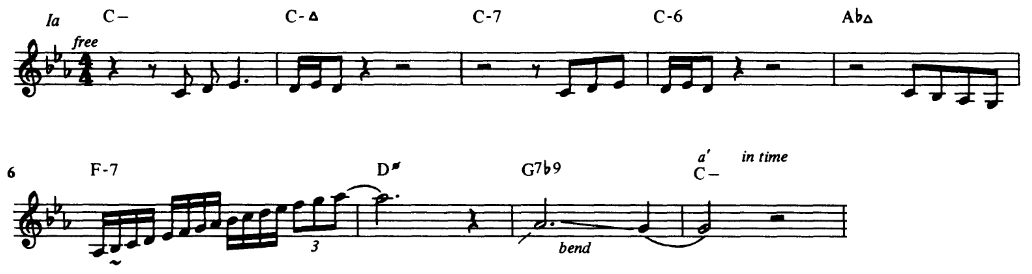
\includegraphics[width=.9\textwidth]{images/chapter1/davis_valentine1.png}}
            \captionsetup{width=.5\textwidth}
            \caption[First nine measures of Miles Davis' melody statement of ``My Funny Valentine," taken from his 1964 recording. As transcribed by Robert Walser]{First nine measures of Miles Davis' melody statement of ``My Funny Valentine," taken from his 1964 recording. As transcribed by Robert Walser.\footnotemark}
            \label{fig:MyFunnyDavis}
        \end{figure}
            \footnotetext{\autocite[]{Walser_1993}.}

    Here, as in the earlier fifteenth-century examples, notation has the ability to ``speak to'' a jazz performer in a particular way, affording a range of potential gestures to be realized in performance. The distinction between Figures~\ref{fig:MyFunnyOrig} and~\ref{fig:MyFunnyDavis}, both (insofar as the language of jazz is concerned) unmistakably instances of the same ``work-concept,'' demonstrates how broad a field of potential is inferred by the symbols on the page. Naturally, these symbols as originally penned were not \textit{deliberately} imbued with these affordances by a composer (``top-down''). Rather, precisely \textit{how} the notation speaks to a performer is contingent on a number of factors---in this example, on Davis' formal training in the western notation paradigm, his experiences with jazz instructors, his countless hours transcribing past performances, his personal taste, etc. While at the time of the cited performance, Davis was undoubtedly ``off book,'' having committed the tune's skeletal framework to memory and no longer requiring printed music in order to faithfully perform his rendition, the $\langle$skeletal framework $\rightarrow$ field of potential$\rangle$ model still obtains. That is to say, a performer unfamiliar with the tune might, when presented with its framework in the form of melody and lead-sheet symbols, arrive at a similarly-structured rendition.


    It is these lead-sheet symbols (e.g. $C^{\Delta}$, $C^{-7\flat5}$, $C^{\circ}$, etc.) which form one of the most salient, concrete points of departure from ``traditional'' (read: nineteenth-century) notation and toward a new, now decidedly Afro-diasporic hybrid model of notation-mediated musicmaking. Mark Abel, in a much-needed 2016 paper on these symbols' history and function traces their origin from their aforementioned ancestral beginnings in figured-bass notation and \textit{alfabeto} (a sixteenth-century derivation of lute tablature) to their formal introduction in the 1920s in popular music charts meant for amateur consumption, then finally to their modern-day use in jazz performance contexts. Per Abel, George Goodwin's ``TuneDex'' cards---bundles of Rolodex-like notecards sold via a mail-in subscription service which featured simplified versions of popular melodies and their attendant chord symbols---were such an overnight success that their sparse notational language became \textit{de rigueur} for jazz and pop musicians across the industry.\autocite[28]{Abel_2016}
    
    These three-part glyphs which indicate an operant chord's root, quality, and extensions (without regard for inversion) were originally employed as labor-saving devices---that is, as a means to obviate any knowledge of tonal harmony on the part of rhythm section players. These were (and still are in pop music compendia) often  accompanied by fingering diagrams for ukulele, guitar, or banjo such that the performer need not possess basic musical literacy in the traditional sense---merely an understanding of the fundamental mechanics of their instrument. However, for Abel, because these chord symbols represent a new layer of abstraction in between the harmony underlying a composition and that harmony's reification in sound, they also afford players a ``radical openness'' in performance, permitting 
    
    %Something weird wrong with the citaton in this paragraph?
        \begin{smallquote}
            new expressive possibilities, and [...] new creative relationships between individuals and collectives capable of eroding the profound schisms between composer and performer, producer and consumer, which have bedevilled the sociology of music in Western modernity.\autocite{Abel_2016}
        \end{smallquote}

    To wit, once chord symbols became part of the standard operating procedure for the composition, dissemination and performance of jazz, he claims, musicians began further conceiving of their improvisations as part and parcel of a harmonic ``grid'' wherein changing chordal fields pertinent to the melody proceed as time progresses. Rather than viewing them as limiting factors which impinge upon improvisatory freedom, Abel sees chord symbols as creative mediators which ``[open up] the rapid `vertical' development of musical harmony,'' facilitating ``alterations and substitutions'' hitherto inconceivable under earlier, more fixed paradigms of harmonic notation. Further, the liberation of the chord progression from a nineteenth-century conception of hierarchical structure \textit{via} these abstract symbols permitted a departure from the notion of a singular key center in both composition and improvisation; paving the way for pieces like the (in)famous middle-period works of John Coltrane (``Giant Steps,'' ``Countdown,'' et al.) which flit liberally from temporary tonic to temporary tonic.
    
    In ``Radical Openness,'' Abel stops short of drawing any particular musico-ethnographic conclusions regarding the widespread adoption of the lead-sheet symbol in jazz performance. At the risk of verging into hermeneutics, I would put forward that perhaps we ought to interpret the rise of the lead-sheet---arguably the most important integration of art music and open notation since the decline of figured bass---not solely as a happy accident stemming from the decline of musical literacy in the early twentieth century, but also as an \textit{active assimilation} of old-guard Eurocentric musical knowledge by a growing pool of artists working in a relatively young Afrocentric paradigm. In essence, the lead-sheet served as a new musical technology developed via a fusion of the now ``fully-fixed'' European art music notation and the mediated openness of Afro-diasporic o/aural practices. That such a fusion could be catalyzed by such a ``low-brow,'' utilitarian notational device as the chord symbol rather than, say, by a concerted effort on the part of some great musical innovator should not go without mention.

    Each chord symbol (as employed by the jazz improviser) serves as a sort of map of a particular harmonic territory; one which applies to the melody of a tune (insofar as it, like a figured bass symbol, indicates which sort of harmony ought to be played underneath the recited melodic line) as well as, canonically, to the harmonic structure of the improvisation which follows. As they progress, each glyph ``projects'' a particular field of potential musical action into the mind of the performer. As with the other open notation schemes we have observed thus far, players are then able to make informed musical moves via a combination of pre-performance data (musical upbringing, personal taste, spoken instructions) as well as the creative constraints on the page. 

    As such, I take it that this experience does not fundamentally differ from the phenomenology of the figured-bass interpreter and thus does not represent some profound new modulation of the performer/composer relationship (as perhaps the genres' very different sonic traces would imply). However, lead-sheet interpretation is particularly interesting in that it represents an instance of ``parallel evolution'' (albeit one displaced by a few hundred years) with the aforementioned figured bass (and/or \textit{alfabeto}, etc.) insofar as it rose to prominence as a musical technology out of a similar necessity: the need to disseminate and perform vast quantities of new music by equally new, less literate sectors of the musical public as well as the need to save material and labor on copying and music publishing. The lead-sheet differs, however, in that, per Abel's claims, it was able to exceed its humble origins and form a key part of the corpus of the new American art music \textit{non plus ultra}, ultimately facilitating a new sort of harmonic conception of musical forms and thereby paving the way for the myriad harmonic languages with which jazz musicians express themselves through to the present day.

    Given the rapid adoption and prevalence of this new musical technology by the end of the second world war, one might expect to see its use somehow reflected in the score-making practices of more traditional art-music composers. Ultimately, though, while jazz (in several understandings of the term) would absolutely have an outsize impact on the new ``classical'' music of the mid-twentieth-century, jazz's lead-sheet model of open composition would never be imported wholesale. However, the 1950s and 1960s \textit{did} bring with them a veritable explosion of innovative and highly individualistic new modes of composition which in turn required attendant new forms of notation. In this chapter's final section, I will examine what I take to be the most historically impactful of these, including, crucially, the extent to which they were (or indeed were not) expressly tied to jazz's ethos, structure, and notational reforms.

   
    %\begin{notestuff}
    %\begin{enumerate}
        %\item Jazz was open before it was notated. Therefore to the extent that it uses notation, it uses OPEN notation. As we saw our c.s.l. and figured bass examples, scores in jazz performance represent ``unfinished'' skeletal frameworks which, if performed, would represent particularly impoverished renditions of the works they represent.

        %\item These frameworks tend to be perhaps more open still than were earlier figured bass structures and tunes may be ``stretched'' often to incredible lengths while still retaining their core identity as an instance of a particular musical work. {Walser Miles Davis excerpt here.}

        %\item What's the wrap-up here? Make a claim about this rebirth of openness impacting avant-notation. Or at least claim that it's hard to make claims.
        
   %     \end{enumerate}
   % \end{notestuff}
    
    \section[Postwar: new open musics]{Postwar: new open musics}

    As I hope has been demonstrated by this point, the histories of our numerous literate art musics are replete with examples of notation having been modified or invented wholesale to suit some material need in the composition, distribution, learning, and performance of musical works. Indeed, the concert music of the mid-twentieth century was no exception. To the contrary, new forms of open music taken together formed a crucial ``reaction formation'' (if you'll permit the analogy) against the rising tide of serialist compositional practices which by that time were \textit{de rigueur}; serving as the received language of European-style avant-gardism.\autocite[14--5]{Taruskin_2009d}

    This is of course not to claim that this new interest in musical openness was entirely coextensive with a new fervor for creative notations. Many noteworthy pieces were constructed which eschewed the romantic fixity of sound-concept using little more than traditional notation---albeit occasionally modified to better suit its new purpose. Before it was amended and republished, Luciano Berio's original \textit{Sequenza} (1958) (excerpted in Fig.~\ref{fig:sequenza}) experimented with flexible ``proportional'' rhythmic notation\footnote{Paul Griffiths identifies this as `space-time notation,' though I've not heard the term elsewhere.} and Terry Riley's standout \textit{In C} (1964) (Fig.~\ref{fig:inc}) permits performances which widely vary in personnel, duration, etc. by employing short modular units of traditional notation to be repeated \textit{ad libitum} by individual performers.

         \begin{figure}
            \centering
            \fbox{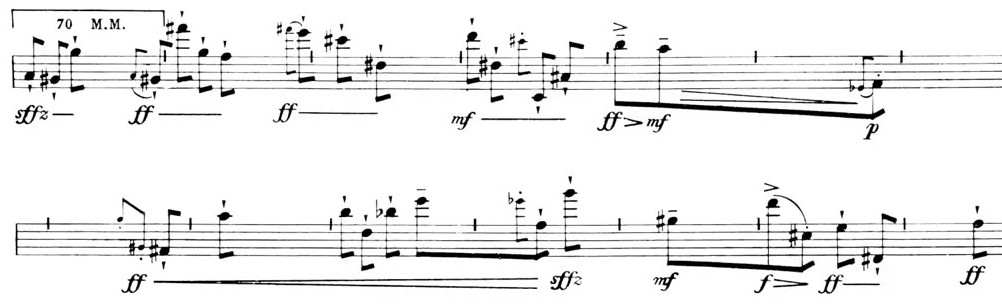
\includegraphics[width=.9\textwidth]{images/chapter1/sequenza1crop.jpg}}
            \captionsetup{width=.5\textwidth}
            \caption[First two systems from the original edition of Luciano Berio's \textit{Sequenza} (I, 1958) which deploys quasi-open proportional notation.]{First two systems from the original edition of Luciano Berio's \textit{Sequenza} (I) which deploys quasi-open proportional notation.\footnotemark}
            \label{fig:sequenza}
        \end{figure}
            \footnotetext{\autocite{Berio_1958}}

            \begin{figure}
            \centering
            \fbox{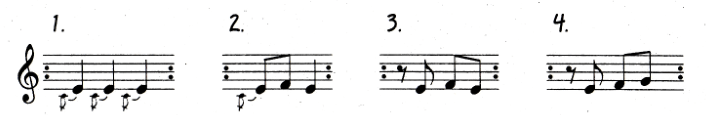
\includegraphics[width=.9\textwidth]{images/chapter1/inc1.png}}
            \captionsetup{width=.5\textwidth}
            \caption[First four modules from Terry Riley's \textit{In C} (1964).]{First four modules from Terry Riley's \textit{In C} (1964). An open score featuring pared-down traditional notation.\footnotemark}
            \label{fig:inc}
        \end{figure}
            \footnotetext{\autocite{Carl_2010}}

    However, insofar as they represent \textit{such} a drastic departure from traditional methods of musical representation, it is often the pieces employing ``neo-notation'' (i.e. any built-to-purpose notation which distinguishes itself from canonical common-practice methods, be it in service of ``open music'' or not) which most captivate composers, musicians, and laity alike. Most authoritative sources point to the earliest days of the 1950s as the beginning of this new compositional mode; specifically citing ``New York School'' composer Morton Feldman as the first to work in this style. Even John Cage, perhaps the best-known composer of open music in this vein, credits Feldman with the style's genesis (though he dubbed it ``[music] indeterminate with respect to its performance'').\autocite{Dohoney_2017} The first system of \textit{Projection 1} (1950), the composition credited with launching this new fervor for open works, is shown in Figure~\ref{fig:feldman1}.

        \begin{figure}
            \centering
            \fbox{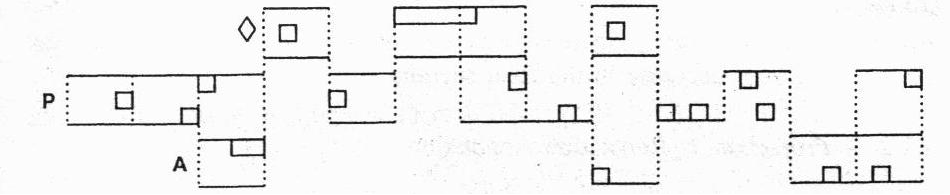
\includegraphics[width=.9\textwidth]{images/chapter1/projection1crop.png}}
            \captionsetup{width=.5\textwidth}
            \caption[First system of Feldman's \textit{Projection 1} for solo `cello (1950). Often cited as the first noteworthy instance of ``graphic'' neo-notation.]{First system of Feldman's \textit{Projection 1} for solo `cello (1950). Often cited as the first noteworthy instance of ``graphic'' neo-notation.\footnotemark}
            \label{fig:feldman1}
        \end{figure}
            \footnotetext{\autocite{Feldman_2002}}

    Though the graphic system he employs seems quite opaque at first blush, Feldman is quite explicit with how his notation is to be interpreted, providing a block of text right at the top of the page:

        \begin{smallquote}
            \textsc{Timbre is indicated: $\diamond$ = harmonic; P = pizzicato; A = arco. Relative pitch (high, middle, low) is indicated: $\overline{\rule{1.2ex}{1.2ex}}$ = high; $\overline{\underline{\rule{1.2ex}{1.2ex}}}$ = middle; $\underline{\rule{1.2ex}{1.2ex}}$ = low. Any tone within the ranges indicated may be sounded. The limits of these ranges may be freely chosen by the player. Duration is indicated by the amount of space taken up by the square or rectangle, each box (\myline[dashed]  \myline[dashed]) being potentially 4 icti. The single ictus or pulse is at the tempo 72 or thereabouts.\autocite{Feldman_2002}}
        \end{smallquote}

    Here, Feldman cedes absolute control over some traditionally fixed musical parameters (pitch, duration) while maintaining control of others (timbre, instrumentation, order of events). The radical break from tradition posed by the ``graphics'' used to represent these events belies the fact that the work is only slightly ``further open'' than many earlier, more conventionally-notated works (e.g. similarly ``proportional'' seventeenth-century unmeasured preludes of the form shown in Figure~\ref{fig:nonmesure}). Only with regard to the pitch axis is Feldman's work truly phenomenologically distinct from these earlier works: a performer must now creatively decide (a) (pre-performance) what range to assign to the upper/lower bounds of each box and (b) (in-the-moment) precisely which pitch in that range to execute during each event.

    Feldman would continue, over the next few years, to develop his ``graph'' compositions alongside his more traditional works, including forays into pieces for larger ensembles like \textit{Intersection 1} (excerpted in Figure~\ref{fig:feldman2}) which grants an additional axis of autonomy to performers by giving them the opportunity to place their attacks at any point in the time segments demarcated with dotted verticals.

        \begin{figure}
            \centering
            \fbox{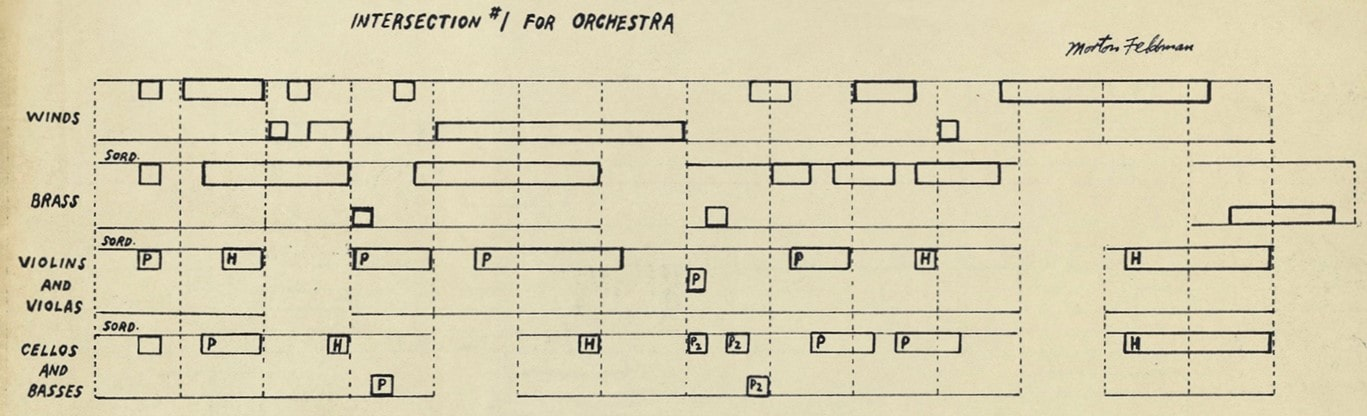
\includegraphics[width=\textwidth]{images/chapter1/feldmanintersectioncrop.jpeg}}
            \captionsetup{width=.5\textwidth}
            \caption[First system of Feldman's \textit{Intersection 1} for full orchestra (1951). Another early ``graphic'' work.]{First system of Feldman's \textit{Intersection 1} for full orchestra (1951). Another early ``graphic'' work.\footnotemark}
            \label{fig:feldman2}
        \end{figure}
            \footnotetext{From a 1962 publication cited in \autocite{Dohoney_2017}}

    Of course, Feldman did not conceive of this new means of representation in a vacuum. His New York School peers John Cage, Earle Brown, Christian Wolff, and associate performer/composer David Tudor similarly sought musical indeterminacy via ``graphic'' notations during this period. However, despite the fact that these composers are frequently cited in the same breath (of which I, too, am now guilty), their motivations for and implementations of neo-notation sometimes differed greatly. Of primary note is Earle Brown's \textit{Folio}, a set of seven pieces penned shortly after Feldman's series of works and published in 1953 which took a remarkably different tack.\footnote{\textit{Folio} is now most often referenced as \textit{Folio and 4 Systems} thanks to a more recent publication which tacks the latter piece to the end of the collection.} Brown, formally trained for many years as a jazz musician, was perhaps more eager (or at least less reluctant) to, with the help of a more active interpreter, co-author his compositional efforts.\autocite{Ryan_2002} As such we find in \textit{Folio} a variety of new symbolic structures which vary in their familial resemblance to traditional notation. Figure~\ref{fig:brownfolio} provides excerpts of the first three pieces from this series, \textit{October 1952}, \textit{November 1952}, and quite possibly the most-reproduced ``graphic'' score extant, \textit{December 1952}.

    %\footnote{I will continue to self-consciously place the term ``graphic'' notation in scare quotes as the word is far too vague to be deployed as often as it is in relevant literature. It's commonly used to refer to techniques as disparate as Xenakis' very precise percussion scores (which feature only very little creative latitude), Cardew's \textit{Treatise} (which is in essence entirely a work of graphic art which only incidentally produces music), Ligeti's \textit{ex post facto} ``listening score'' for \textit{Artikulation} (never meant to be used for performance, only perusal), and Xenakis' pre-compositional material for \textit{Metastasis} (not a score at all). I much prefer, whenever possible, to use more precise language to disambiguate these very different uses for ``graphics'' in the context of music representation.}

        \begin{figure}
            \centering
            \fbox{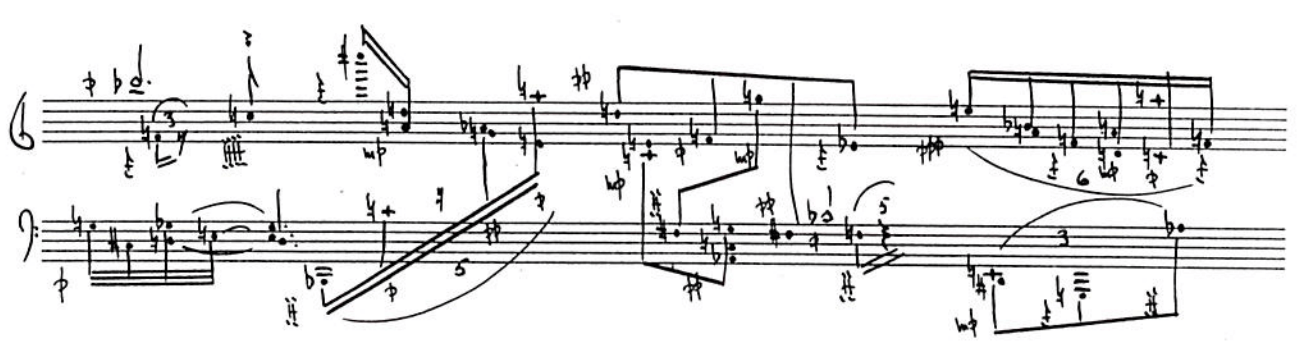
\includegraphics[width=.7\textwidth]{images/chapter1/oct52.png}}

            \vspace{5pt}
            
            \fbox{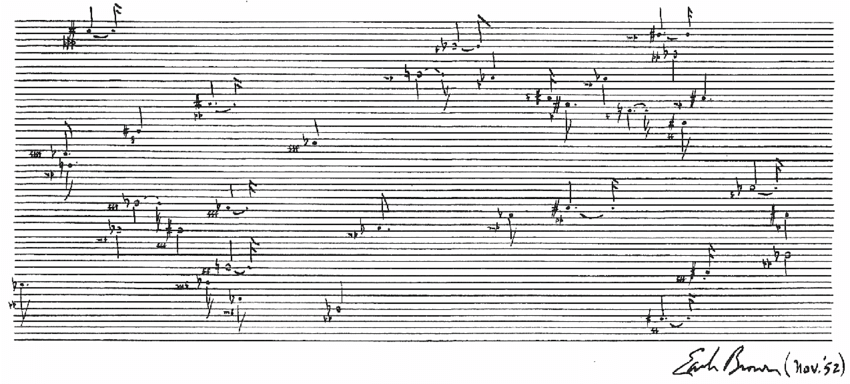
\includegraphics[width=.7\textwidth]{images/chapter1/nov1952.png}}

            \vspace{5pt}
            
            \fbox{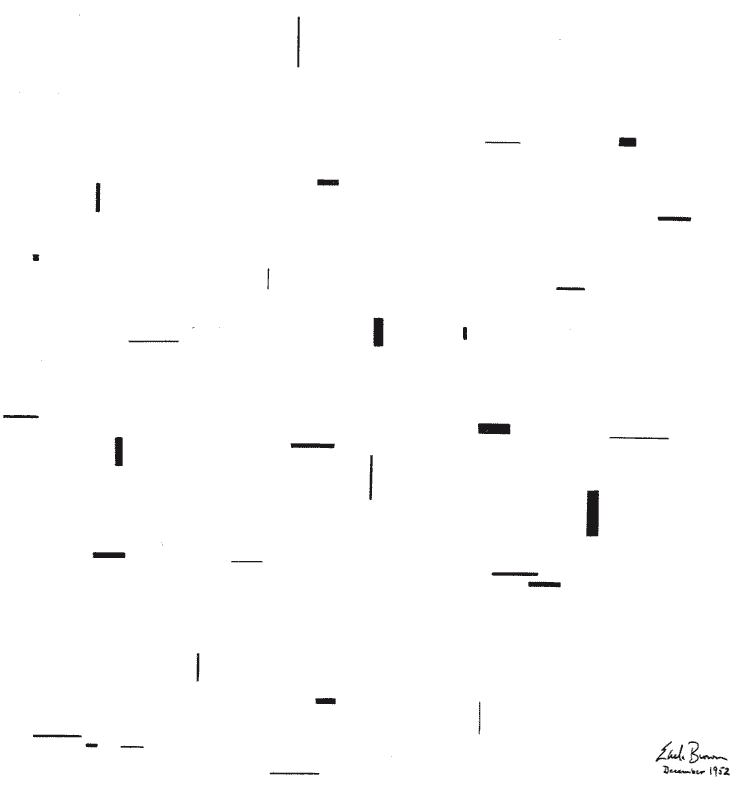
\includegraphics[width=.5\textwidth]{images/chapter1/dec52.png}}
            \captionsetup{width=.5\textwidth}
            \caption[Excerpts from Earle Brown's \textit{Folio} (1953). From top to bottom: First system from \textit{October 1952}; Entirety of \textit{November 1952}; Entirety of \textit{December 1952}.]{Excerpts  from Earle Brown's \textit{Folio} (1953). From top to bottom: First system from \textit{October 1952}; Entirety of \textit{November 1952}; Entirety of \textit{December 1952}.\footnotemark}
            \label{fig:brownfolio}
        \end{figure}
            \footnotetext{\autocite[2--8]{Brown_1986}}

    That scores of this heterogeneity were composed within mere months of each other and published as one package speaks, perhaps, to the sense of newness and experimentalism that led to their creation. \textit{October} (for piano), despite its somewhat whimsical engraving and lack of barlines, was given a standard metronome marking of $\crotchet$ = 135 and was intended to be performed ``straight-ahead.'' \textit{November} (marked ``for piano(s) and/or other instruments or sound-producing media'' and given the alternate title ``Synergy'') maintains at least a tenuous relationship to traditional notation in that it still employs traditional dot/stem/flag notation with accompanying dynamic markings. However, the instructions provided with the score give an entirely different perspective:

    \begin{smallquote}
    The frequency range will be relative to that of each instrument performing the work. \textit{To be performed in any direction from any point in the defined space for any length of time}. Tempo:\textit{ as fast as possible to as slow as possible [...] inclusive}. Attacks may be interpreted as completely separated by infinite space, collectively in blocks of any shape, or defined exactly within that space. Lines and spaces may be thought of as tracks moving in either direction (horizontally at different and variable speeds) and clef signs may be considered as floating (vertically over the defined space) [...]\textit{ The defined space may be thought of as real or illusory, as a whole or in parts}.\autocite[1]{Brown_1986}
    \end{smallquote}

    Like Feldman, Brown permits the vertical compass of the ``graphic'' to map to the range of the performer's instrument. Unlike Feldman, though, who only \textit{further abstracted} the representation of musical events in time, Brown here has shattered one of the most fundamental principles of western music notation which had held steadfast since at least the era of Guido d'Arezzo: the mapping of time to the \textit{x}-axis. Play no longer proceeds \textit{top left} $\rightarrow$ \textit{bottom right} but rather ``proceeds'' in a manner entirely up to the performer's discretion. What information Brown's bespoke notation actually \textit{provides} a performer, then, is actually rather vague. Horizontal lines which typically demarcate precise pitch quanta have become indefinite signifiers of ``vertical'' distance. The notes' forms (shape, stems, flags) have, in light of his careful instructions, become virtually empty of concrete meaning. We might assume that, insofar as they remain unmentioned in the notes, dynamic markings are meant to be observed ``as written''---in which case they would serve as the sole fixed parameter in the piece save the number of attacks. Even without consulting firsthand accounts of the piece's creation; taking this evidence together it becomes clear that Brown has begun centering the ``visuality'' (or ``aesthetic,'' if you like) of his glyphs over and above any denotative symbolic value they might otherwise provide. In a crucial inversion, this visuality now drives the sound-concept and the production of sound---completely contrary to the traditional state of affairs where a composer chooses symbols for their denotative content in order to bring about a desired sound-concept.\footnote{
        Certainly, a number of earlier examples could be said demonstrate a sort of privileging of notation's aesthetic in composition---most notably minor composer Baude Cordier's ``Belle, bonne, sage'' which renders a fifteenth-century chanson in the shape of a heart. Even Telemann, in his \textit{Gulliver Suite} experimented with ``eye music'' which similarly wrapped conventional sonic products in a visually arresting package. These, while of limited historical interest, do not, to my mind, prefigure the explosion of new ``visual composition'' in mid-twentieth century.
        }
    This new orientation toward the visual promptly reaches its apotheosis in \textit{Folio}'s third piece: \textit{December 1952}---by far Brown's most well-known work. Having been inspired by Alexander Calder's ``mobile'' sculptures which bear no one consistent visual trace, Brown writes (emphasis his):

    \begin{smallquote}
         The performer was asked to consider these [graphic] elements in this manner only at the moment---and they could be changed continually [...] So, \textit{December 1952} was generated from that very early concern with trying to create something which was a \textit{score} comparable to a visual mobile.\autocite{Brown_2008}
    \end{smallquote}

    While it is often spuriously claimed that \textit{December} was proffered entirely without performance directions in a sort of Dadaist flourish (frequently by authors who ought to know better), in fact at the time of its 1953 publication its instructions reproduced in full read thus:\footnote{Inexplicably, Paul Griffiths makes the claim that of indeterminate scores, \textit{December 1952} was ``at once the earliest, the most enigmatic (there being no instructions about how these shapes are to be realized as sound)'' found in \autocite{Griffiths_2011}}

        \begin{smallquote}
            The composition may be performed in any direction from any point in the defined space for any length of time and may be performed from any of the four rotational positions in any sequence. In a performance utilizing only three dimensions as active (vertical, horizontal, and time), the thickness of the event indicates the relative intensity and/or (where applicable instrumentally) clusters. Where all four dimensions are active, the relative thickness and length of events are functions of their conceptual position on a plane perpendicular to the vertical and horizontal planes of the score. In the latter case all of the characteristics of sound and their relationships to each other are subject to continual transformation and modification. \textit{It is primarily intended that performances be made directly from this graphic ``implication'' (one for each performer) and that no further preliminary defining of the events, other than an agreement as to total performance time, take place.} Further defining of the events is not prohibited however, provided that the imposed determinate-system is implicit in the score and in these notes.\autocite[1]{Brown_1986}
        \end{smallquote}

    Here Brown helpfully provides for two distinct modes of play. The first (in my experience the most frequently adopted method) retains the overall strategy described in \textit{November}, only with the piece's glyphs abstracted one degree further from traditional notation; indicating duration with horizontal extension and dynamic with stroke thickness rather than a \textbf{\textit{pp}}/\textbf{\textit{ff}}-style glyph. The second, perhaps more opaque option has the performer imagine a virtual plane extending from the page. What appear to be two-dimensional rectangles are actually projections of three dimensional objects at various distances from the viewer along this \textit{z}-axis. In either case, Brown makes clear that no preconceived direction-of-play is meant to obtain and that the page may be rotated in any of the four cardinal orientations pre-performance. 
    
    We should note that where earlier improvisation-oriented scores left the precise boundaries of their openness (i.e. the breadth and depth of notation's fields of potential) up to the training and good taste of their performers, Brown (and to a lesser extent Feldman) take great pains to reify these boundaries in prose to be considered prior to performance. By explicitly granting performers the opportunity to choose between multiple interpretive schemes, Brown forges a new sort of relationship between composer, performer and score---one conveyed not through traditional pedagogical/experiential channels but one defined \textit{in situ} by the composer himself.
    
    I have taken, perhaps, a disproportionate amount of time to discuss these early neo-notational works (despite the fact that Feldman quickly abandoned these ``graphic'' forays in favor of a return to traditional work which only \textit{felt} improvisatory) for one important reason: By way of these first forays, these two composers, Feldman and Brown, have articulated (albeit imperfectly) the primary paradigmatic rupture between two classes of open ``graphic'' scores which persists in some form to the present day. We might sum up this coarse division in the following tree diagram (Fig.~\ref{fig:soundvimage}):

        \begin{figure}
            \singlespacing
            \centering
            \begin{forest}
                forked edges,
                for tree={parent anchor=south, child anchor=north,draw,align=center,edge={-latex}}
                [\textsc{new compositional}\\\textsc{openness/``indeterminacy''}
                 [traditional\\notation
                    [{ex: \textbf{\textit{In C}}\\(1964)},tier=word]
                    ]
                 [neo-notation
                  [``sound-first''\\neo-notation
                    [{ex: \textbf{\textit{Projection I}}\\(1950)},tier=word]
                    ]
                  [``image-first''\\neo-notation
                    [{ex: \textbf{\textit{December 1952}}\\(1952)}, tier=word]
                    ]
                 ]
                ]
                \end{forest}
            \captionsetup{width=.5\textwidth}
            \caption{One articulation of notation paradigms during the ascendance of new open musics in the mid-twentieth century.}
            \label{fig:soundvimage}
        \end{figure}

    Works which seek to explore new (or indeed return to old) open forms fall into two broad categories: those which modify (often by paring down) traditional notation and those which introduce new notations for the purpose. Though there is certainly more nuance to be found than is represented here, this latter group tends to divide into two ideologically distinct further categories: Scores which begin from sound- (or process-) concepts which hope to attain an imagined sound world or creative procedure via a novel method of encoding (i.e. ``sound-first'') and those which hope to elevate some visual object (e.g. \textit{December 1952}'s line-segment array) to the status of a \textit{sounding} object; posing it to the performer(s) as an open question of interpretation (i.e. ``image-first'').\footnote{Of course, this could never be a hard-and-fast boundary. There is no reason to imagine that Feldman wasn't to some degree motivated by the sheer novelty and appearance of his new symbolic language or that Brown did not hear an abstract \textit{klangwelt} in his head which motivated \textit{December}. Based, though, on Brown's repeated appeal to visual inspiration and metaphor, I think this is a reasonably safe, if blunt, assessment.} 

    These two approaches are drawn into even more stark contrast when one considers their underlying motivations. It is telling that by 1954, Feldman had entirely abandoned his prolonged experiment with graph (his term) scores, evidently on grounds that they ``liberat[ed] the performer'' to too great a degree. While his scores achieved their initial goal of allowing for an unpredictable, non-replicating sonic trace which did not rely on his particular tastes, habits, and conditioning, Feldman was clearly dissatisfied with the extent to which his performers' creative autonomy crept into the works.\autocite[99]{Taruskin_2009d} Despite an errant indication in his graph score \textit{Marginal Intersection} (1951) for a player to perform a line ``as in a jazz ensemble,'' Feldman clearly did not share in the ethos of jazz musicians who, too, deployed novel notation mechanisms in order to promote a new form of open music.\autocite{Dohoney_2017}

    This jazz-avoidant (occasionally jazz-hostile) orientation among America's hypermodern art-music composers forms one of the primary motivations behind George Lewis' much-cited paper ``Improvised Music after 1950: Afrological and Eurological Perspectives'' and certainly extends to John Cage who, even more frankly than Feldman, denounced the creative processes underlying jazz improvisation, distancing his own ``indeterminate'' works from it whenever possible. Lewis hypothesizes that despite this consistent denunciation, the performance practices which emerged during this period of New York School flourishing are inextricably bound up in the radical musical advances made by America's \textit{other} modernist school of composition: jazz (bebop in particular---not coincidentally also ``headquartered'' in New York City during the 1950s). Lewis sees this reluctance to own up to the clear parallels between these two open musics as essentially rooted in a creeping form of anti-Black racism which tainted the artistic efforts of Black Americans as ineluctably low-brow, unserious, or backward-facing.\autocite{Lewis_2002} 

    To be sure, not to say every New York School associate was equally dismissive of the Afrological avant-garde. Earle Brown himself, a professional jazz trumpeter prior to his turn toward concert music, speaks candidly of the extent to which jazz performance practice motivated the form and content of his open works. From a 1991 interview:

        \begin{smallquote}
            \begin{itemize}
                \item \textbf{BD (Bruce Duffie):} Was the notation your own, or was the notation borrowed from other people that discovered it first?
                \item \textbf{EB (Earle Brown):} No, it was completely my own. I first started doing these things in 1951 and '52, and what occurred to me, from a jazz background, was the freedom and the flexibility that jazz has from performance to performance.
                \item \textbf{BD:} Yes. They're never the same. They're improvisatory.
                \item \textbf{EB:} They're never the same twice. But if you play \textit{How High the Moon} seventeen times, you know that it's \textit{How High the Moon}, even though it's never, in detail, the same twice. That excited me.

                \centering
                    \noindent\rule{2cm}{0.4pt}
                    
                \justifying
                \item \textbf{EB:} [...] But what occurred to me as an ex-jazz musician was why can't the variations be a function of the interaction of the musicians with the material that I have composed? One of the greatest things about jazz is the instant, instantaneous communication.  One played [sings a line] and then the other one goes [sings an answering line].  It’s like you and I having a conversation where we exchange ideas.  That’s always one of the most beautiful things to me about jazz.  So that’s what I tried to introduce, and this goes all the way back to your first question — why new notation, and why the scores look different than other people’s scores.  It’s because I want to introduce the possibility of the musicians not only playing what I write, but interacting like a human family of friendly people.\autocite{Duffie}
            \end{itemize}
        \end{smallquote}

%    \begin{notestuff}
%        Amend this statement to put it more in line with M's reading of Lewis.
%    \end{notestuff}

    \noindent Here, Brown highlights that crucial aspect of jazz performance cited in the previous section: the seemingly infinite malleability of its work-concepts. Given that Brown undoubtedly experienced this malleability via the same notation mechanisms jazz players employ today (i.e. via open melodies and chord symbols), I think it is no great logical leap to suggest that this ``Afro-diasporic return'' to open forms significantly impacted his decision to ground his music in a new notation. While Brown's frankness with regard to this line of influence appears to be the exception rather than the rule, it nevertheless serves to illustrate productive cross-talk between these two musical paradigms---an important byproduct of which were the notation schemes at the heart of this research.


\section{Conclusion}

    With greater and greater intermingling of (``classical,'' ``jazz'', ``free improvisation'') art music spheres in the twenty-first century, more open scores are being composed today than ever were during the 1950s and '60s. The large-scale ``democratization'' of the avant-garde thanks to art's newfound accessibility on the internet has led, I think, to a measure of mainstream acceptance of the viability of the open score as part of the art music landscape. Even ``mainstream'' institutions now occasionally admit these radically open works into their repertoire (albeit usually those by the now-venerated New York School composers themselves). Given that we are at a local apex of the production and consumption of notation-mediated open music, and given that the variety of o/aural-literate traditions underpinning the creation of these works is now more diverse than ever, the comparative lack of rigorous analysis and critique of these fascinating works is somewhat startling. When discussions of notation-mediated open music \textit{do} appear (either in lay-facing publications or in ``the literature''), authors often demonstrate a lack of interest in investigating precisely what sets one open work apart from the rest. 

    That is to say: despite the fact that ``graphic score'' and ``graphic notation'' are common terms of art familiar to anyone who has completed a college-level music history sequence, these terms are wholly inadequate to describe the broad swath of notation-mediated open musical works. I take it that there is an important difference-in-kind between these ``image-first'' (by far the most prevalent and most-discussed form of open ``graphic'' scores) and the often more intellectually knotty but lesser-appreciated ``sound-first'' open works. These two broad categories display radically distinct initial motivations, construction methods, performance phenomenologies, and attendant structures of performer/composer agency. There have been very few concerted attempts to elucidate these differences, to categorize works \textit{according} to these aspects, to taxonomize the varieties of open musical work, or to highlight trans-historical parallels between these and other musics.

    The following chapter will take on the much-needed task of (a) describing in more detail the varieties of notation-mediated open music in terms of these motivations, methods, structures of agency, etc., specifically focusing on these under-discussed ``sound-first'' composition techniques and (b) addressing the few incisive scholarly efforts which lay the foundations for a greater understanding of these works.


% \begin{notestuff}
%     \begin{itemize}
% %\item worth mention that the feldmanian approach is directly tied to a fundamental mistrust of performer agency, given that in 1954 Feldman would abandon his new notation on ground that it ``liberat[ed] the performer'' to too great a degree. This betrays a fundamental sort of ideological opposition to the basic experiences of jazz performance practice---one famously shared by Cage.

% %On the other hand, the Brownian model was developed by a jazz musician who seemed much less reluctant to admit the biases, habits, tastes of his performers into the body of his own works. This seems noteworthy

% %\item writers callously lump these things together, but it's critical to a more thorough understanding of how notation mediates performance to really pull these apart! in the next chapter i'll blah blah

% \item discussion of the mistrust of ``improv'' in denotative graphic scores like Feldman's sets up the uniqueness of somebody like Braxton who does use denotative notations but does so in service of improv rather than despite it.
%     \end{itemize}
% \end{notestuff}

% FOR DISCUSSION OF NOV + DEC and FELDMAN's instructions
%\begin{notestuff}
    %\begin{itemize}
    %\item I'm spending so much time on these earliest scores because they stand in for the fundamental schism in neonotations that I'm getting into in ch. 2 and they form the model for essentially all notational-exploratory works which follow in coming decades.

    %\item By all accounts feldman's works sought a particular sound-world
    
    %\item Brown's approach was visual first, per his citing Calder
    
    %\item if one thing sums up this era of notational practice, it's that now musics are being composed which place notation in the driver's seat -- experiments with the VISUAL are changing our attendant SOUND WORLDS rather than the reverse (what accounts for this?)

    %\item This explosion is of course intimately tied up with (though not coextensive with) a parallel new interest in open musics of all flavors (indeterminacy, improvisation, aleatory)

    %\item Obviously fascination with the visual and a linking between visual and aural creativity are not a new phenomenon -- historical examples do exist which ``privilege'' the visual. However nothing compares to the visual experimentalism that characterized the mid-century.

    %\item Accounts of the motivations behind these innovations differ drastically. Firsthand accounts by often fairly forthright composers point to a number of influences. A certain intellectual tradition argues that this new open music craze is \textit{essentially} downstream of Afrocentric improvised music traditions --- while I think there's real merit to these arguments and a hermeneutic sense in which they hold water, I think the real story is more complicated  

    %\item in fact there are SO many new methods of notation that we begin to suffer from a lack of vocabulary with which to differentiate them. they tend to all get lumped in under the category ``graphic notation,'' which is too broad a category to be of any use.                                                                                 
    %\end{itemize}
%\end{notestuff}

%%%%%%%%%%%%%%%
% END COPY %%%$
%%%%%%%%%%%%%%%


\chapter{Toward a Richer Typology of (Open) Notations}
%%%%%%%%%%%%%%%
% START COPY %%
%%%%%%%%%%%%%%%

%\epigraph{\selectlanguage{german} \glqq Die Existenz von Mischformen bedeutert jedoch nicht, daß die Trennung von »Zeichen« und »Zeichnung« verwischt werden soll. Im Gegenteil: Daß innerhalb der Mischformen der Zeichenanteil und der graphische Aspekt sich trennen lasses, zeigt gerade, daß es sich um zwei grundverschiedene Kategorien handelt.\grqq \selectlanguage{english}}{György Ligeti, 1965}


\epigraph{\singlespacing ``The existence of mixed forms does not, however, mean we ought to blur the division between ``sign'' and ``illustration.'' On the contrary, the fact that the sign component can be separated from the graphic aspect [...] is itself a demonstration that we are dealing with two fundamentally different categories.''}{György Ligeti, 1965, tr. Edmund Griffiths.}


%    \small
%    \begin{itemize}
%        \item \texttt{\textbf{\textcolor{red}{red = construction notes}}}
%        \item \texttt{\textbf{\textcolor{blue}{blue = I want this somewhere but maybe not here?}}}
%        \item \texttt{\textbf{\textcolor{ForestGreen}{ForestGreen = an idea that, to the best of my ken, is mine}}}
%    \end{itemize}
%    \normalsize

%\section{Introduction}

    In the previous chapter, I used a rapid historical gloss to illustrate an important narrative arc in Western art music's technological development. Specifically, I aimed to chart the ebb and flow of notation's relative sonic determinacy---the openness and fixity of our shared musico-graphic signs. While much of this effort was dedicated to tracking changes in the common practice notation serving as most literate musicians' lingua franca, the final section of the chapter addressed a few of the varieties of new notation which seemed to spring up \textit{ex nihilo} in the 1950s and 1960s. To my mind, the most interesting and under-analyzed of these and subsequent new notations feature robust encoding schemes which provide specific shape and color to a musical work---while at the same time permitting a great deal of creative latitude on the part of the work's interpreter(s).
    
    This chapter is ultimately intended to address the analytic issues posed by the arrival of these bespoke ``open'' notations and to move toward new ways of thinking about their form and function which avoid the murky, obscurant language often featuring in their discussion. To wit, the specific goal I have set for this chapter is the development of a working typology of notations; one able to fold in the variety of traditional methods of music encoding, but one specifically aimed at disambiguating the variety of extant open notations so prevalent in the composition of the twentieth and twenty-first centuries. Only so armed may we then begin to make sense of the more complex open works which spurred on this research---works which may operate on many simultaneous levels of fixity, employing several different encoding schemes over the course of a single piece, a single section or a single measure.

    To that end, I'll begin by discussing what I take to be the most pressing issues facing our clear-eyed assessment of music notation, moving from most general to most specific. Specifically, I'll first address our ``common-sense'' notion of notational semantic content; putting forward a new way of thinking about notation-as-symbol so as to find a shared vocabulary with which to discuss both traditional and neo-notation on the same terms. Next, I'll interrogate concepts of openness in music composition; specifically highlighting common takes on the ``open work,'' generally, and on ``graphic notation,'' which I take to needlessly complicate our understanding of this notation's function. Following this, I will highlight those few scholarly efforts which seem to take positive steps toward our goal---with special emphasis on a critically under-cited essay which I think does a great deal of the work in describing our desired typology. Ultimately it is this source which I'll use to catalyze the development of a refined model.


\section{Base-level function of music notation}

    \begin{smallquote}
        In music notation, sounds are represented by small circles (or ovals) called notes. Notes can be high or low, and they can be short or long. The higness [sic] or lowness of the note is its pitch. To represent high and low pitches, notes are placed high or low on the staff, the five horizontal lines going across the page.\autocite{Wood_2015}
    \begin{center}
    \noindent\rule{1cm}{0.4pt}
    \end{center}   
        Notation is a recognised system of symbols (essentially marks on paper) that visually represent a music or sound idea. Standard notations are well-known, clearly defined structures that are able to communicate sound information in a functional and precise manner.\autocite{debbielyddon_2015}
    \begin{center}
    \noindent\rule{1cm}{0.4pt}
    \end{center}
        Printing music on a page allows a composer to convey information to a musician who will ultimately perform that composer’s work. The more detailed the musical notation, the more precise a performer will be. In this sense, musical notation is no different from printed text.\autocite{Music_101}
    \begin{center}
    \noindent\rule{1cm}{0.4pt}
    \end{center}
        \end{smallquote}
        
    As promised, I would like to begin by revisiting a few of our initial assumptions given at the beginning of the last chapter, specifically as regards the foundations of the function of music notation and of its potential to mediate musical performances. The ability to meaningfully consider complex new works which often combine several distinct varieties of notation in a single score is entirely contingent on an understanding of what, at a basic level, these notations are doing---i.e. what they encode and transmit.
    
    I provide the above inscriptions as an interesting  sampling of the variety of extant definitions of ``music notation.'' The above public-facing, decidedly non-academic definitions were specifically chosen for the way they seem to get at the ambient, unexamined sense of what it is we use notation \textit{for}. It is particularly interesting to note their discrepancies: The first takes notation to directly refer to sounds---though it is unclear whether these are meant to be virtual or real---and makes sure to include the mapping between spatial dimensions on the page and height in frequency space. The second mentions ``music-'' and ``sound-ideas'' as potential referents for notation, though does not go into detail as to their differences. Here, notations are structures for the communication of this sound data from composer to performer such that the performer, having formed a clear mental image of what sound the composer is seeking, will be able to bring it into being. The third, on the other hand, does not refer to sound at all. Like the second, it emphasizes that notation is a means of information conveyance between a communicator and communicatee. However, precisely what \textit{sort} of information notation actually bears is left unspecified. Interestingly, it also immediately appeals to our notion of precision---implying that there exists some ideal virtual music toward which notation aims; carrying with it the implicit goal that performers should get as close to it as possible. These represent three distinct ways of thinking about our everyday interactions with music notation---none of which, alone, allow us to describing using uniform vocabulary the manifold forms of notation we observed in the last chapter.
    
    David Gutkin, in a paper I'll return to later in this chapter, hints at a sort of solution:

        \begin{smallquote}
            But might not any musical notation and not solely particular avant-garde scores or tablature be understood as the prescription of action rather than, or at least as well as the coding of sound? Even if notation does not always mimetically or analogically depict physical movements \textit{per se}, culturally significant graphic marks are only ever operative as imperatives to act.\autocite{Gutkin}
        \end{smallquote}

    In the following section, I will argue for just such a model of notation-interaction---one which de-centers common notions of sound-signification in favor of mediation of fields of potential musical action. The aim of this model is not to replace common parlance or overturn centuries of received wisdom pertaining musical inscription at large, but rather to enable a more precise discourse---especially as regards complex, multiform neo-notation that characterizes so many fascinating works today. 
    
    \subsection{Notation as imperative to act}
    
    To begin with, I will refer back to Mieko Kanno's definition with which we began the previous chapter. Per Kanno, music notation serves generally to ``describ[e] musical works and giv[e] specific instructions for them to be realized.'' Earlier, I refined (genericized) this definition slightly by allowing that music notations merely be coherently ``oriented toward an existing [...] or virtual [...] musical product'' given that there exist many music notations which were never intended to allow for realization of a work (Rainer Wehinger's famous \textit{ex post facto} ``graphic'' score for György Ligeti's \textit{Artikulation}, for instance). While these definitions served as a good launchpad for our discussion, neither of them give any idea as to the mechanism by which notation ``describes'' or is ``oriented'' toward sonic products. Though the article itself is fairly comprehensive, the head-line definition in the \textit{Grove} entry for ``Notation'' is similarly vague. For its primary author, Ian Bent, notation taken whole is simply some ``visual analogue of musical sound, either as a record of sound heard or imagined, or as a set of visual instructions for performers.''\autocite{Bent_2014} Elegant, broad-level definitions like these necessarily fail to get us any closer to an understanding of the objects to which elements of music notation actually refer. For that, we must turn to discussions of notational semiotics. Luckily, a good starting point is not far away. In a later section of the article, Bent elaborates:

        \begin{smallquote}
            A musical notation requires, in essence, two things: an assemblage of ‘signs’ and a convention as to how those signs relate to one another. A written musical notation requires further a spatial arrangement of the signs on the writing surface that makes a ‘system’ of the assemblage; it is this system that forms an analogue with the system of musical sound, thus enabling the signs to ‘signify’ individual elements of it.\autocite[Section II.1]{Bent_2014}
        \end{smallquote}

    This strikes closer to the heart of the question. Here Bent establishes the position that music notation (taken whole) serves as a ``visual analogue'' of actually-existing music. A system of notation comprises signs (what I've been generically calling ``glyphs'') and a syntax through which those signs are perceived and understood. Implicit in Bent's argument, though, is the assumption that the sound-system's referents (signified by the assemblages which form our notations) are \textit{themselves} sounds. 
    
    To clarify: Per the paradigmatic ``standard'' model of composition: A composer conceives of music in some way and represents it in a score, then hands it off to a performer who creates music using the score as a sort of ``recipe,'' hopefully satisfying everyone in the process. Semantically speaking, though, the score serves as a sort of black box of representation---while it's clearly desirable that a score (as an individual entity) should bear some representative orientation toward some body of sound, either past, future, or potential, it is not altogether trivial precisely what the composer is encoding and sending and precisely what the performer is receiving when this process of representation takes place. Given the definitions we've seen, one might naïvely imagine that (i) a composer simply conceives of ``pure sound,'' in some arrangement, (ii) determines which symbols from his repertory would be best to represent that sound and commits them to paper, after which (iii) a performer interprets these symbols---similarly taking them as signifying particular sounds which they must dutifully bring into existence. The performer then realizes these sounds of the type and ordering the composer intended and everyone is happy. This model, however, has some critical flaws which expose the inadequacy of the notion that music notation somehow represents sound in the way that a noun represents a person, place, or thing.\footnote{
        Let us be clear that sounds (as they actually exist) are physically- and temporally-extended \textit{things}---highly complex and specific in form. I take it that even the strictest ``sound-semanticist'' would not argue that the familiar glyphs on the page are meant to refer to some \textit{specific} sound (e.g. of the form \{A442 at 80dB begun March 9th 1972 at 14:30:26 and ending March 9th 1972 at 14:30:27.5\}. Rather, I take it that they would argue that the symbol on the page directly refers to some internally-audiated sound which bears a reasonable resemblance to some sound \textit{also} familiar to the performer.
        }
    
    First, it is often the case that a composer does not intend a particular sound at all, but what we might generically call a ``process''---for instance some harmonic function. If I write B$^{\flat-7}$ on the lead sheet I'm composing, it's not because I'm imagining some particular sound, but because I desire harmonic functionality of a particular form from my rhythm section or soloist. Fulfilling that harmonic role faithfully could yield any number of resultant sounds---any of which would satisfy the composer. Similarly, a composer might intend not a sound, but a particular sort of physical gesture \textit{irrespective} of what sound results. Figure~\ref{fig:pression} illustrates an excerpt culled from Helmut Lachenmann's brilliant \textit{Pression} for unaccompanied 'cello, which, per Paul Griffiths ``is typical of Lachenmann's work of this period in its concentration on irregular techniques, and thereby on the physical mechanism by which the sounds are produced.'' Below, we see his novel proportional notation which specifies the non-sounding movement of the left hand separately from the sounding movement of the bow. Given that an audience member three rows back from the performer may not even be able to hear the thin, breathy sound emitted, it is not too far flung to imagine that Lachenmann penned this gesture for the theatricality of its movement rather than for the precise attributes of its sonic byproducts. Here, neither the intent nor that which is transmitted by the notation is sound proper.\autocite{Griffiths_2011}

        \begin{figure} 
            \centering
            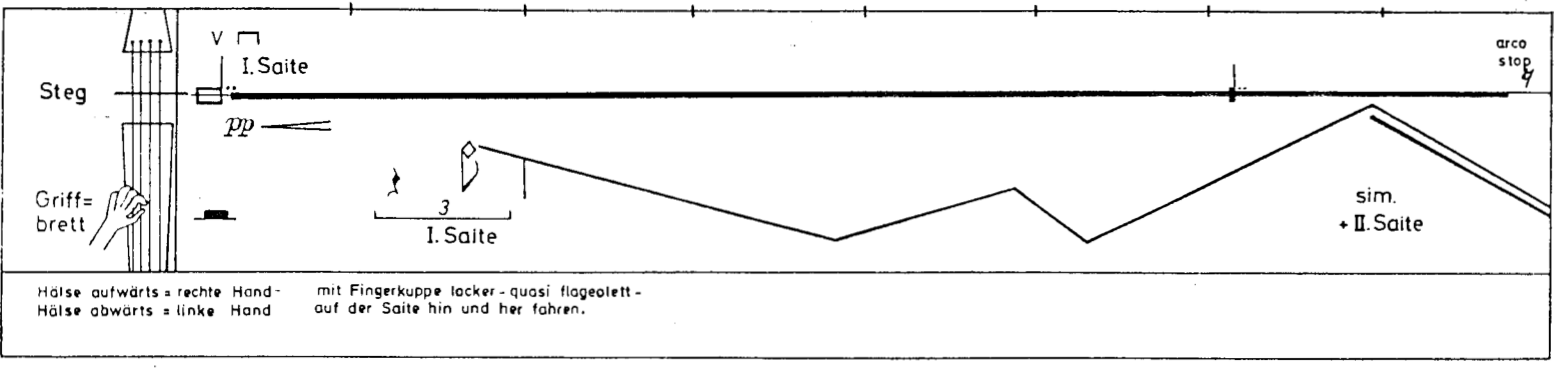
\includegraphics[width=.99\textwidth]{images/chapter2/pression1.png}
            \captionsetup{width=.5\textwidth}
            \caption[First system of Helmut Lachenmann's \textit{Pression} (1969) demonstrating non-sounding ``gestural'' notation (lower jagged line) which modifies sounding notation (upper solid line).]{First system of Helmut Lachenmann's \textit{Pression} (1969) demonstrating non-sounding gestural notation (lower jagged line) which modifies sounding notation (upper solid line).\footnotemark}
            \label{fig:pression}
        \end{figure}
            \footnotetext{\fullcite[]{Lachenmann_1969}}

    Indeed, especially in contemporary music there are many such symbols which clearly yield sound via their interpretation but for which we would struggle to clearly identify a sonic referent. What ``sound'' is indicated by a figured-bass symbol? Likewise, what ``sound'' is indicated by the boxes in Feldman's \textit{Projections} series? The rectangles in \textit{December 1952}? Further, if notation is to refer specifically to concrete sounds it becomes non-trivial to define the inner workings of ``more fixed'' or ``more open'' notations---categories which clearly function  in practice. Sound (at least under our common usage of the term), whether imagined or issued, cannot be any more or less fixed than it is. A sound is merely an end product of the process notation inscribes. Simply put, our common-sense understanding of notation's ``fixity'' or ``openness'' can not obtain if we take notations to formally refer to sounds proper. In this light, I would like to tentatively put forward an alternative model of notational semantics in order to facilitate discussion of the open works at the core of this project. The following is a semi-formal elaboration of my argument:

    % \begin{notestuff}
    %     (unsure of the best way to format this... I want to illustrate the logical flow, but maybe bullets/numerals are too strange...)
    % \end{notestuff}

    \begin{center}
    \noindent\rule{3cm}{0.4pt}
    \end{center}   

        \begin{itemize}[leftmargin=*, label=--]
        
        \item Music notation is typically used to generate or archive music. It seems correct that music notation, properly arranged, should by and large \textit{represent} in some way its resultant musical products (i.e. virtual or actually-existing sounds). A score---some meaningful, cohesive arrangement of notation---serves as a ``recipe'' allowing for the creation or recreation of an imagined complex of sounds extended in time. We might think of the score, its encoding procedure, and its resultant (or potentially resultant) sounds as together forming a conceptual whole. An important misconception which might arise from this ${score} \rightarrow {music}$ mapping, though, is that individual glyphs \textit{congruently} map to individual sounds---i.e. that there exist one-to-one mappings between units of notation and the expected sounds which ought to result from their reading.
            
        \item During the encoding process, symbols are chosen by a composer (from a repertory of such symbols) on the basis of their results---i.e. the sounds, gestures, or procedures which would result from their interpretation. However, we should be very cautious about making the claim that the symbols are chosen because they necessarily \textit{refer directly} to some desired sounds.
            
        \item The score's downstream sonic products, after all, only result in practice via some interaction (be it a tight or a loose reading) between a performer and the notation provided by the composer. The performer's body and instrument stand between score and sound---thus the glyph \{$\vcenter{\hbox{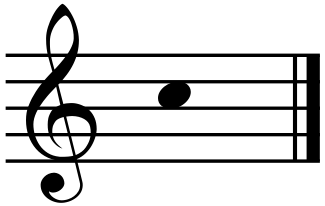
\includegraphics[width=1.2cm]{images/chapter2/c5raw.png}}}$\} in practice does not ``neutrally'' stand in for some platonic, un-sounded C5, but rather results in a C5 as brought into existence by some sounding body. As a convenient shorthand, we think of it as referring to raw pitch data, but insofar as we are discussing notation oriented toward \textit{performance}, this is not the case.
            
        \item For instance, it should be unambiguous that the individual note-glyph \{$\vcenter{\hbox{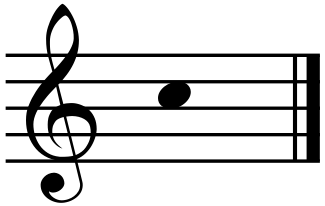
\includegraphics[width=1.2cm]{images/chapter2/c5raw.png}}}$\} does \textit{not} refer to a sound. Given the traditional understanding of how music notation syntax works, there's not enough information to reproduce a particular imagined sound from the information given. However, in many literate music traditions, perfectly valid scores might be constructed entirely of such ``bare'' notes, as is the case with many of the works in Anthony Braxton's ``Ghost Trance Music'' series (see Figure~\ref{fig:ghosttrance1}).
    
        \begin{figure} 
            \centering
            \fbox{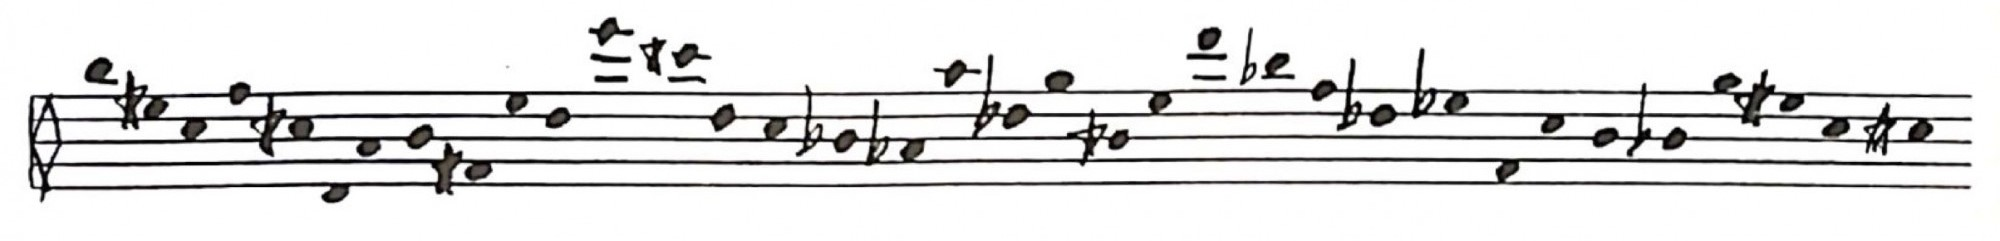
\includegraphics[width=.9\textwidth]{images/chapter2/ghosttrance2.jpg}}
            \captionsetup{width=.5\textwidth}
            \caption[Excerpted system from Anthony Braxton's \textit{Composition No. 193} which features long stretches of unadorned noteheads and bespoke ``diamond'' clefs and ``star'' accidentals.]{Excerpted system from Anthony Braxton's \textit{Composition No. 193} which features long stretches of unadorned noteheads and bespoke ``diamond'' clefs and ``star'' accidentals.\footnotemark}
            \label{fig:ghosttrance1}
        \end{figure}
            \footnotetext{Reproduced courtesy of \fullcite[]{Cauwenberghe_2021}. Due to the complex nature of Braxton's graphic titles, I will be abbreviating them as necessary with his self-imposed catalog numbers.}
    
        \item One might assert instead that notation refers to specific sounds only when enough clear information is provided (per the rules of our system as we understand it) to fulfill the ``recipe'' with a particular instrument and with a particular tempo and dynamic. After all, I can much more clearly imagine the sound which would result from \{$\vcenter{\hbox{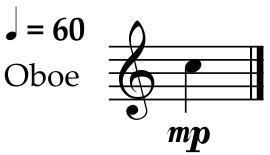
\includegraphics[width=2cm]{images/chapter2/c5oboe.png}}}$\} than from its unadorned cousin.
            
        \item Unfortunately, this is still an insufficient model. Humans cannot realize symbols identically each time; even with this greater degree of specificity, there will always be discrepancies (even large discrepancies) between repeated realizations. Each symbol or complex of symbols either explicitly or implicitly carries with it a degree of latitude as to what constitutes a valid or acceptable realization. \{$\vcenter{\hbox{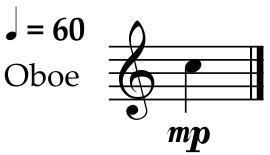
\includegraphics[width=2cm]{images/chapter2/c5oboe.png}}}$\} might be cut off 20 milliseconds short of the mathematically called-for duration, it might be flat or sharp by 10 cents, it might be slightly louder or softer, it might be performed with light or no vibrato, etc.
            
        \item It is therefore impossible to point to any particular sound which serves as the referent for any complex of music-notation symbols. As such, I would like to propose an alternative model; specifically, one in which notation's referent is instead conceived as a virtual set of sound-producing actions which could plausibly result from the notation's rendering in performance. In the previous example, the glyph-complex \{$\vcenter{\hbox{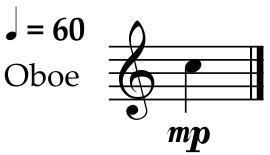
\includegraphics[width=2cm]{images/chapter2/c5oboe.png}}}$\} would refer to a set which includes all of the given potential realizations as well as any others which would be considered faithful. I'll use the term ``field of potential'' (FOP) to refer to this set of appropriate realizations which serves as the referent to a notational glyph.
            
        \item As such, we no longer need to adorn a bare \{$\vcenter{\hbox{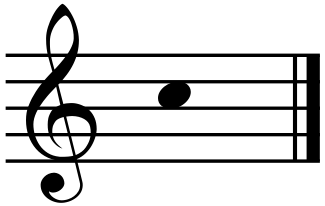
\includegraphics[width=1.2cm]{images/chapter2/c5raw.png}}}$\} (which would and has served as a structurally-complete notation all by itself) with all of these other symbolic trappings (dynamic, tempo, etc.) in order to meaningfully describe a referent for a particular glyph. The bare C5's referent, in other words \textit{contains} the referent of \{$\vcenter{\hbox{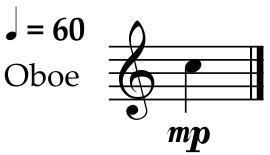
\includegraphics[width=2cm]{images/chapter2/c5oboe.png}}}$\} as well as any other potential realization of \{$\vcenter{\hbox{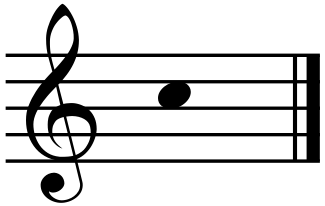
\includegraphics[width=1.2cm]{images/chapter2/c5raw.png}}}$\}.
        
        \end{itemize}

    \begin{center}
    \noindent\rule{3cm}{0.4pt}
    \end{center}   

    Of course, this argument itself raises some important questions. What, first of all, defines the scope and content of this field of potential action? If we are to suspend our notion that somehow notational glyphs map one-to-one with intended sounds, we must at the same time adopt a new model of how notation-mediated communication \textit{works}. As with any semantic content, notation's field of potential is multiply determined via a complex of (i) the ``encoder's'' intent, (ii) the code regulating the sign's usage, and (iii) the recipient's reading of the sign. On the part of the composer, the FOP is defined by some intentional \textit{sound- or process-concept} (S/PC) which he encodes to the best of his ability using the glyphs at his disposal. Under this model, the process (for a typical sound-concept) proceeds as follows:

        \begin{smallquote}
            \begin{itemize}[label=--]
                \item A composer internally audiates a sound for oboe, based on his past experience of ``oboeness,'' (i.e. develops a sound-concept) and decides to encode it for a performer to reproduce.
                \item He must then ask himself two things:
                    \begin{enumerate}
                        \item Does the chosen glyph's implied FOP include the sound he has audiated?
                        \item How much discrepancy between his audiated sound and the actual performed sound would be permissible?
                    \end{enumerate}
                \item If the chosen glyph's FOP contains the imagined sound \textit{and} allows only for permissible discrepancy given the established code agreed upon by composer/performer, then the glyph suffices.
                \item If, on the other hand, the glyph's FOP contains the imagined sound, but the potential discrepancy between audiated sound and performed sound is too great, the composer must further \textit{restrict} the FOP in some way---either with additional symbolic modifiers (\textbf{\textit{mp}}, $\quarterNote$=60, etc.) or with verbal/textual instructions.
            \end{itemize}
        \end{smallquote}

    Crucially, this procedure holds true independent of the degree of fixity inherent in the system of notation. If music notation were to somehow point to sound directly, we would have to posit entirely different modes of signification between ``closed scores'' which refer directly to fixed, predictable virtual sound and ``open scores'' which grant the performer some degree of latitude in realization. That certain notations, be they systems or individual glyphs, permit more leniency in interpretation (i.e. are more open) should be uncontroversial. This being the case, though, we would need a way of describing the represented sound as \textit{itself} being more or less definite depending on whether its associated sign were open or closed---ultimately an unenviable position when compared with the simpler alternative. Below I have prepared two time-oriented ``flow'' diagrams illustrating the standard composer/performer interaction---one under the ``naïve'' model (Fig.~\ref{fig:naïvediagram}) and one under my amended model (Fig.~\ref{fig:amendeddiagram}). Translations of the relevant relationships follow the figures.\footnote{
        A couple of caveats for these interaction charts: First, this is meant to be a model illustrating the simplest possible composer/notation/performer interaction---it does not purport to represent \textit{all} such interactions. In practice, obviously, there are complex feedback mechanisms (e.g. player feedback in rehearsal, inter-musician communication, etc.) which would change the whole interaction structure. 
        
        Second, this is meant to be an interaction between a composer and a \textit{single} performer. The model could just as well be expanded to include an arbitrary number of agents but for the purposes of illustration I thought it best to keep things as simple as possible. 
        
        Third, I marked $S^*_P$ optional for the fact that, it seems, we could conceive of a scenario where the performer ``mechanically'' reproduces notation which they are capable of executing but which is too complex to audiate inwardly. Alternately, the composer may have encoded a process-concept which is likewise reproducible by the performer but which is so opaque it fails to reveal itself conceptually. In either case, a ``reflected'' sound/process-concept is not strictly necessary for the model; hence the broken line.
        
        } 

%        \begin{notestuff}
%            I need a small paragraph here or at least a generous footnote describing the role of ``syntax'' in the amended model I put forward below. It just comes out of nowhere and does a lot of work. Also, I drew an ``influence arrow'' from ``syntax'' only to the gamma-complex. But shouldn't it kind of point everywhere??
%        \end{notestuff}

        \begin{figure} 
            \centering
            \fbox{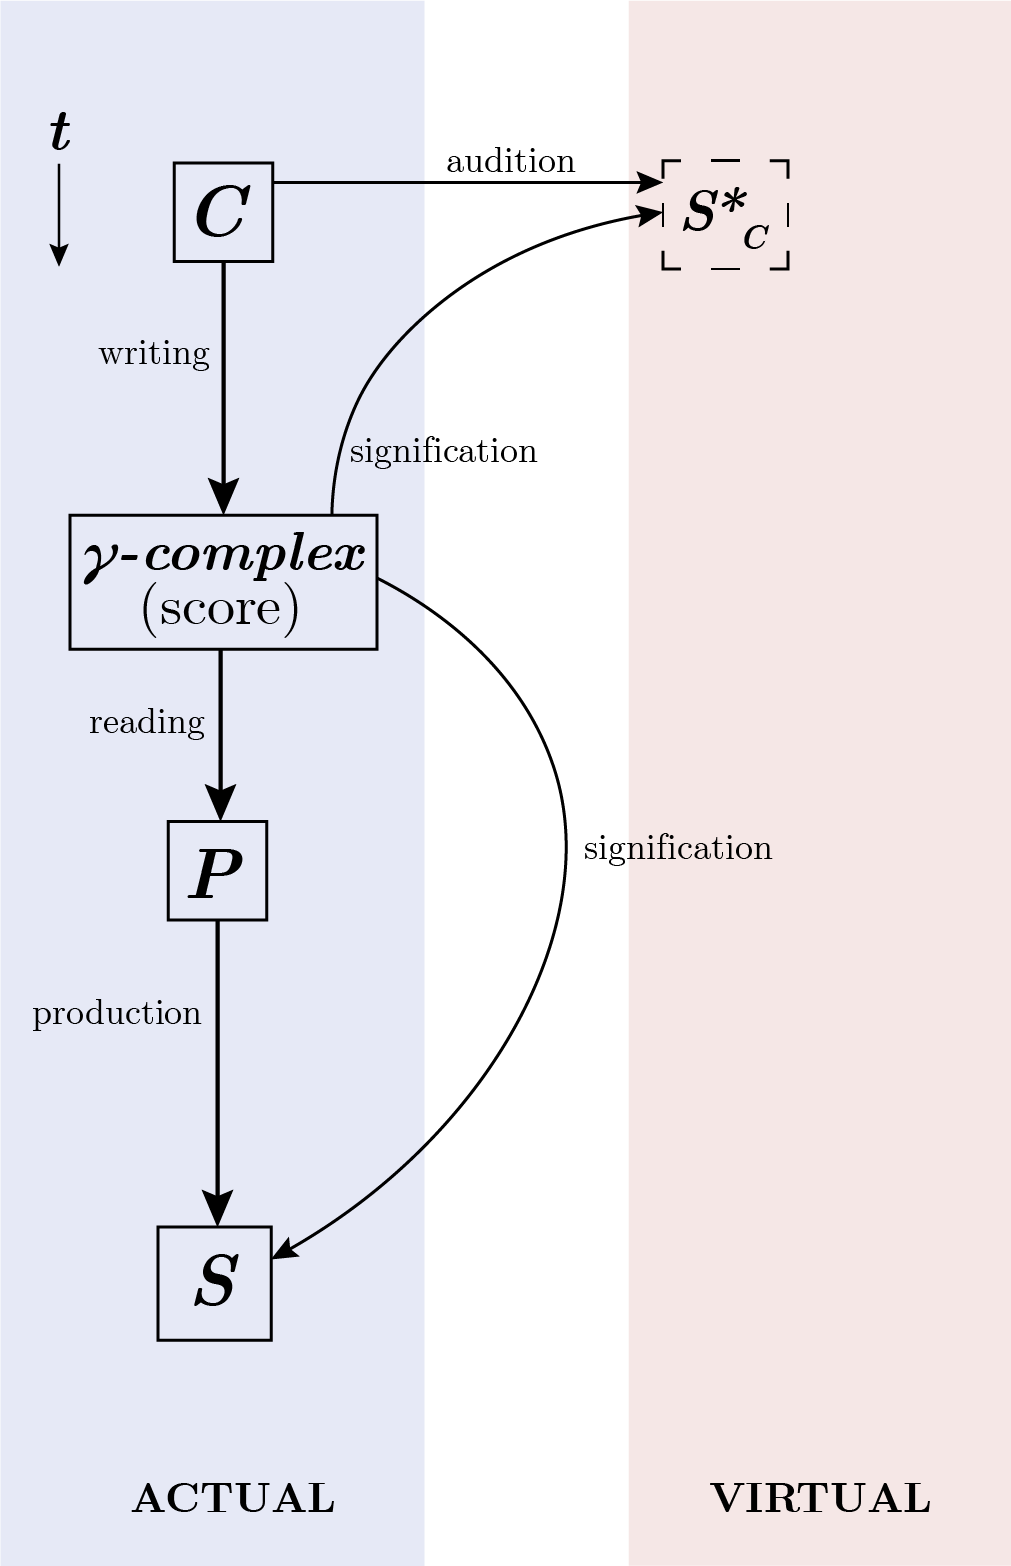
\includegraphics[width=.5\textwidth]{images/chapter2/2-3x.png}}
                
                \begin{smallquote}
                    \begin{center}
                        \textit{``Naïve'' Process}
                    \end{center}
                
                    \begin{enumerate}
                        \item A composer ($C$) \textbf{audiates} a sound-concept ($S^*_C$) which s/he wishes to realize in sound.
                        \item S/he \textbf{writes} the score---a complex of glyphs ($\gamma$) intended to yield the imagined $S^*_C$ at some future time.
                        \item A player ($P$) \textbf{reads} the score, forming a mental image which matches that devised by the composer ($S^*_C$).
                        \item $P$ then \textbf{produces} corresponding sound $S$.
                        \item To the outside observer, $\gamma-complex$ \textbf{represents} the final sound $S$ produced as well as the sound concept $S^*_C$ originally devised.
                    \end{enumerate}
                \end{smallquote}

            \captionsetup{width=.5\textwidth}
            \caption{``Naïve'' notation interaction model.}
            \label{fig:naïvediagram}
        \end{figure}

            
        \begin{figure} 
            \centering
            \fbox{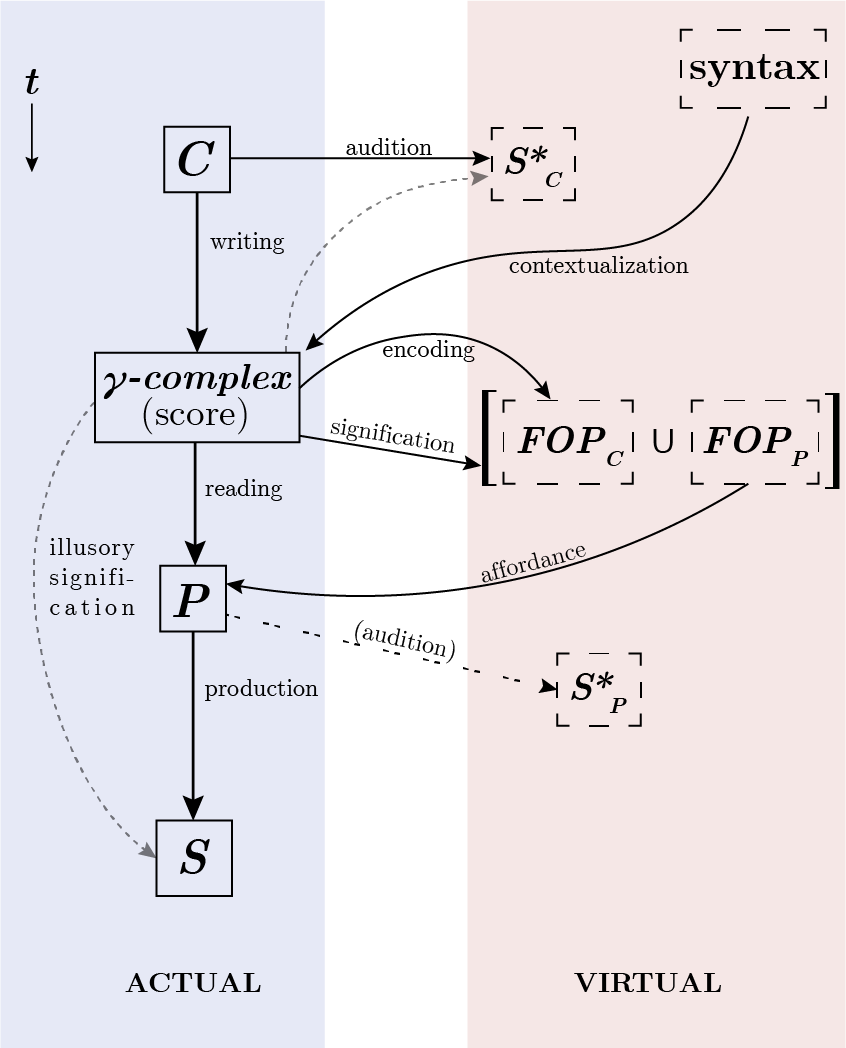
\includegraphics[width=.65\textwidth]{images/chapter2/signification_diagram_fix.png}}
                
                \begin{smallquote}
                
                    \begin{center}
                        \textit{Amended Process}
                    \end{center}
            
                    \begin{enumerate}
                        \item Syntax \textbf{organizes} the whole interaction and is familiar to both composer ($C$) and performer ($P$), whether it is part of the received structure of music notation or newly communicated in the score.\footnotemark                            
                        \item $C$ \textbf{audiates/devises} some sound/process-concept ($S^*_C$) which he would like to hear $P$ perform.
                        \item $C$ \textbf{writes} the score---a complex of glyphs ($\gamma$-complex)---such that  their realization might bring about an instance of $S^*_C$. (That is, such that a field of potential $FOP_C(\gamma)\Rightarrow S^*_C$ where ``$\Rightarrow$'' is a relation meaning ``fulfills'').
                        \item $P$ \textbf{reads} $\gamma-complex$, which affords him/her $FOP_P$.
                            \begin{enumerate}
                                \item To an outside observer, $C$'s $\gamma-complex$ can then be said to represent the union of $FOP_C$ and $FOP_P$.
                                \item $P$ may him/herself \textbf{audiate/devise} $S^*_P$ such that $S^*_P \approx S^*_C$, though it's not strictly necessary.
                            \end{enumerate}
                        \item $P$ executes $\gamma-complex$, selecting a gesture $g$ (such that $g \in FOP_P$), which \textbf{produces} sound.
                    \end{enumerate}
                \end{smallquote}

            \captionsetup{width=.5\textwidth}
            \caption{Amended notation interaction model.}
            \label{fig:amendeddiagram}
        \end{figure}
            \footnotetext{ 
                        One final qualification: Where elsewhere I have attempted to be as precise as possible when choosing the language with which to describe these notation-interaction models, here I have somewhat callously included the catchall module labelled ``syntax'' as a way of hand-waving the many \textit{a priori} factors which influence the way notation is used to encode/decode music. To be more specific, I take this ``syntax'' to be a global variable comprising, for instance, (a) the extent to which the composer and performer were formally trained in the use of the notation scheme, (b) their musical upbringing (Am I to play these triplets the French or Italian way?), (c) personal taste (How furious is \textit{furioso}?), (d) the notation's graphic trace (How well is the piece engraved? Are the symbols legible?), as well as many other factors. Naturally there will always be some discrepancy (ranging from inconsequential to game-changing) between the composer's received syntax and the performer's based on their entirely distinct lived experiences.
                                    
                        In addition, I have drawn an arrow from ``syntax'' to the $\gamma$ complex in order to depict (very generally) the way these syntactic elements influence the artifact that is the score, though perhaps it would be more correct to point this directional influence at the ``audition,'' ``writing,'' and ``reading'' processes themselves.
                        }

    Per my earlier comment, it should go without saying that this amended view of notation-signification is not meant to supercede the common-sense way we talk about or interact with notation in the course of our everyday musical experiences. Instead, couching the content and function of notation in terms of fields of potential action should allow us to assess complex, multi-notational works (for instance, Anthony Braxton's \textit{Composition No. 76} excerpted in Fig.~\ref{fig:Braxtonex}) with greater clarity; a task I'll be attempting in Chapter 3.

        \begin{figure} 
            \centering
            \fbox{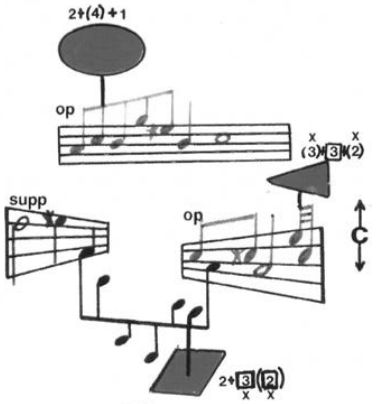
\includegraphics[width=.5\textwidth]{images/chapter2/76no1.png}}
            \captionsetup{width=.5\textwidth}
            \caption[Excerpt of module ``E3'' from Anthony Braxton's \textit{Composition No. 76} (1978) demonstrating multiple concurrent forms of notation operating at several degrees of openness.]{Excerpt of module ``E3'' from Anthony Braxton's \textit{Composition No. 76} (1978) demonstrating multiple concurrent forms of notation operating at several degrees of openness and semanticity.\footnotemark}
            \label{fig:Braxtonex}
        \end{figure}
            \footnotetext{\autocite{Braxton_Comp_76}}

    In advance of this, though, it is crucial that we first consider our received notion of what, precisely, constitutes an ``open work.'' Given that our stated goal is the development of a working typology, it is worth assessing those sources which posit new forms of notation; in practice, usually ones designed for the construction of new, sonically indeterminate works. Writers with insight into these new forms of composition often have views on their attendant notations which are worth examining in greater detail: specifically, the way that they pull apart ``fixed'' and ``open'' notations.

%\begin{notestuff}
%**POTENTIAL OBJECTIONS? The relativistic nature of notation's semantic content?---I guess it was always going to be relativistic. If it communicates sound data, the sound \textit{written} would never exactly match the sound \textit{read}...
%\end{notestuff}


%    \subsection{Fields of potential in practice\\Open notation v. open works?}


    \section{The open work in the literature}

        % \begin{notestuff}
        
        % I think I need a better explanation here of how the previous discussion aids us going forward, placed right before the following section. Something to the effect of:
        % \begin{smallquote}
        % ``There's all these heterogeneous ways of notating music. This type is for sound, this type is for physical movement, this type is for communicating some concept, this kind is open, this kind is fixed. But, we have the option of thinking of all of these as just one type of thing: symbols which constrain in various ways potential action---giving the sets of potential action various attributes. [do anything here as long as it's on the note C] [do anything here as long as it's quarter notes] This means that scores are made of only one type of STUFF which makes it easier to discuss cases where notation is hybridized, nonspecific, very open, etc.''
        % \end{smallquote}
        % From here we can categorize notations differently; perhaps more usefully---not according to their form necessarily, but according to the ways they mediate these fields.
            
        %    %*****In the previous section, I set out to interrogate the notion that notation is best understood as sets of symbols which signify past/present/future sound; posing instead an alternative model which allows us to discuss both ``sounding'' and ``non-sounding'', fixed and open notation alike under a common vocabulary. This was posed in the hope that it might facilitate more detailed discussion of the knottier, more interesting contemporary works which often combine several different types of notation to various ends.
            
        %    %To that end, I would like to first examine a number of canonical scholarly efforts which in one way or another pull apart the compositionally ``open'' from the ``fixed.''
            
        %    %*****If we now proceed based on the assumption that notation represents and operates on fields of potential performer action rather than on sounds themselves, it allows us to make sense of aspects of open scores which would otherwise be difficult to reconcile.
           
        %    %*****Earlier we examined jazz lead sheets and indeterminate New York School scores as paradigmatic examples of open notation and demonstrated how, in practice, their use as performance mediators differed drastically from traditional 19th-century scoring methods. The question arises: using this newfound semantic structure, how might we assess just what makes these common ``open'' works open? After all, under this view (to reiterate my position from Chapter 1), the notion of an open score (to contrast with a traditional fixed score) is merely a helpful fiction: all notation is non-trivially ``open notation'' by virtue of the fact that music performed by human beings (as opposed to the essentially perfect mechanical reproduction of digital audio, etc.) is \textit{necessarily} indefinite. How might it be possible to draw a line between these two varieties of musical experience which, to the performer, invariably feel like two different kinds of phenomena? 
        
        %    %*****In order to better grapple with this question, we'll turn now to two important sources which demarcate this closed/open boundary in one way or another before assessing their concomitant philosophical commitments (implicit or explicit).
        
        %    \end{notestuff}

    \subsection{The open work for Eco}
    
    As far as I am aware, the use of the term ``open'' to refer to certain types of (``indeterminate,'' ``aleatoric,'' ``improvisatory'') artwork dates to Umberto Eco's collection \textit{The Open Work}, published in English in 1989 but comprising essays dating back a further 25 years or so. Here, Eco discusses the many ways a work of art---be it music, prose, sculpture, etc.---may be left ``open'' by its creator, ensuring that it can never meaningfully be represented by only a single vantage point. The open work, for Eco, is still ``unfinished'' at the time it is handed to an interpreter or a reader and requires active participation on the part of the recipient in order for it to reach completion. To be clear, this is not a music-philosophy text; Eco merely uses discussion of the new rush of open compositions as a launch-pad for his analysis of greater artistic trends. As such, the cross-section of musical works he uses as case studies is unfortunately rather narrow. Eco focuses on the musics he knows best---namely, mid-century avant-garde concert music---to the conspicuous exclusion of any Afrocentric open works which were (at time of writing) fully flourishing. Nevertheless, the book remains an important touchstone in the field and as such might aid in our goal of assessing the form and function of performance-mediating notations. Right from the outset, in a chapter dubbed ``The Poetics of the Open Work,'' Eco puts forward his model of musical openness by examining four recent musical works penned by some of the towering figures of mid-century composition---Karlheinz Stockhausen, Luciano Berio, Henri Pousseur, and Pierre Boulez. Each of these works he considers in some way genetically open---``incomplete'' or ``unfinished.'' Of these he observes:

        \begin{smallquote}
            What is immediately striking in such cases is the macroscopic divergence between these forms of musical communication and the time-honored tradition of the classics. This difference can be formulated in elementary terms as follows: A classical composition [...] posits an assemblage of sound units which the composer arranged in a closed, well-defined manner before presenting it to the listener. He converted his idea into conventional symbols which more or less oblige the eventual performer to reproduce the format devised by the composer himself, whereas the new musical works referred to above\footnote{...he specifically cites Stockhausen's \textit{Klavierstück XI}, Berio's \textit{Sequenza} for solo flute, Pousseur's \textit{Scambi}, and Boulez' \textit{Third Sonata for Piano.}} reject the definitive, concluded message and multiply the formal possibilities of the distribution of their elements. They appeal to the initiative of the individual performer, and hence they offer themselves not as finite works which prescribe specific repetition along given structural coordinates but as ``open'' works, which are brought to their conclusion by the performer at the same time as he experiences them on an aesthetic plane.\autocite[2-3]{Eco_Robey_1989}
        \end{smallquote}

    Here, Eco provides a basic framework by which we might understand openness in musical works at large. In short, for Eco, an open work is one which requires ``initiative,'' i.e. active collaboration on the part of the performer in order to bring the work ``to [its] conclusion.'' Open works here function ``like the components of a construction kit,'' with no one canonical assemblage of their parts. Indeed, there seems to be a startling and immediately apparent distinction between canonical works of classical music and these new open forms which demand active, creative decision-making on the part of the performer. Interestingly, Eco expressly rejects the notion that ``openness'' as a property might be applied to \textit{any} scored work which requires the interpretation of a performer in order to truly come into being---arguing instead that open and closed works represent a true difference-in-kind. He claims:

        \begin{smallquote}
            At this point one could object (with reference to the wider meaning of ``openness'' already introduced in this essay) that any work of art, even if it is not passed on to the addressee in an unfinished state, demands a free, inventive response, if only because it cannot really be appreciated unless the performer somehow reinvents it in psychological collaboration with the author himself. Yet, this remark represents the theoretical perception of contemporary aesthetics, achieved only after painstaking consideration of the function of artistic performance; certainly an artist of a few centuries ago was far from being aware of these issues.\autocite[6]{Eco_Robey_1989}
        \end{smallquote}
    
    It seems that for Eco the rigidity of the historically contingent rules and norms with which interpreters of ``closed'' works (Monteverdi, Brahms, Stravinsky, et al.) performed their pieces preclude any sense of openness seeping in through the various unspecified parameters (dynamics, say, or lengths of fermatas) which would be creatively filled-in by the aforementioned composer/performer ``psychological collaboration.'' In traditional, ``classical'' works, ``[w]hat in fact is made available [i.e. left open] is a range of rigidly preestablished and ordained interpretative solutions, and these never allow the reader to move outside the strict control of the author.''\autocite[6]{Eco_Robey_1989} While Eco spends much of the chapter eloquently drawing parallels between open forms as they exist in the plastic arts, literature, drama, etc., I would like to bracket these in favor of examining his perceived dichotomy between (in his terms) ``open'' and ``classical'' works.
    
    For convenience, I'll use ``taste'' as shorthand referring to the suite of musical conventions, unspoken rules, etc. which serve to fill in the gaps of a not-fully-determinate work (e.g. the ``taste'' which determines dynamics in a Bach performance). Certainly, in the same sense that music notation functions positively and prescriptively as a call for a player to act in a certain way, this musical taste is always already present for the performer as a constraining factor. Thus, Eco would argue, a Baroque continuo with figured bass cannot be said to be ``open'' in the same sense as \textit{Klavierstück XI}\footnote{Distinct from the mid-century open works I've discussed so far, Stockhausen's work merely presents the pianist with a number of ``fixed'' fragments of various lengths. The performer must decide where to begin the piece and in which order the fragments will be played.}, since there exists (or at least existed at the time of writing) no particular socio-aesthetic conditioning surrounding the performance of a Stockhausen work. The realization of a figured bass is, in a sense, overdetermined by this conditioning. Where Telemann intended his harpsichord accompaniment (however improvisatory) to function within these bounds of good taste, and therefore held them fixed, so the argument goes, Stockhausen built the notion of performer agency and ``incompleteness'' into his work from the get-go.

    This seems like a strange take. If the openness of a work is entirely contingent on a combination of the composer's intent and some nebulous sense of ``rules-as-understood-at-time-of-writing,'' then, yes, perhaps despite the wide creative latitude Telemann's harpsichordist would have had in the performance of one of his concerti, these pieces could be considered ``closed'' in light of the overwhelming influence of unspoken poietic factors. However, despite much effort on the part of music historians to reconstruct an ``authentic'' Baroque performance practice, the boots-on-the-ground reality of the taste which governed players in Telemann's time is phenomenologically extinct to us. A twenty-first-century performer of Baroque music simply cannot be said to be confined to the same norms as was her eighteenth-century counterpart. The contemporary performer, then, must exercise her own creative agency in deciding precisely which voicings to use for the provided figured bass---agency tempered, certainly, by historical precedent; by the desires of her employer; by the actions of the other musicians on the bandstand; but agency ultimately her own. Thus Baroque continuo is, to the modern performer, a fragment of an open work: one which blends seamlessly in with the more fixed elements of the same piece (rigid metric structures, diatonic scales, etc.). The norms which ``closed off'' the work so long ago no longer exist.

    Further, I am skeptical of the notion that the deliberate measure of openness incorporated into the modern works Eco cites somehow precludes the influence of contemporary aesthetic norms on their performance. In fact, I think it would be more controversial today to somehow claim that canonical works like these could somehow be exempt from these same constraining pressures. Surely the timing of \textit{Sequenza}'s fermatas or the pauses in Boulez' \textit{Third Sonata for Piano}---both factors which Eco takes to be indicative of the pieces' openness---are as much governed by ``preestablished and ordained interpretative solutions'' as are classical cadenzas, etc. Perhaps it's true that classical music aficionados are more stringent than contemporary music critics in their assessments of faithful or authentic performances, granting less leeway in the execution of ``closed scores,'' but certainly we could find a ``wrong way'' to perform the \textit{Sequenza} such that it would merit being corrected by an improved sense of ``taste.''

    Finally, Eco's omission of any of the myriad contemporary Afro-diasporic open works is somewhat troubling. Of course, Eco does not purport to exhaust the world's various open music paradigms, but given jazz's impact on mid-century composition, intellectual discourse, and culture at large, we should expect some reference---even if only a dismissal from the new model of composition he identifies. Jazz is, after all, the preeminent genre for which works are ``brought to their conclusion'' by some performer who radically co-creates the final sonic product even as she ``experiences them on an aesthetic plane.'' While we could feasibly imagine a sort of platonic notion of one of Bach's keyboard works, for instance, it is definitionally impossible to conceive of Charlie Parker's early 1949 performance of ``Cardboard'' without taking into account the way in which Parker himself completes the work in the very moment of its realization. 

    That is to say: the performance of a Bach piece is easy to perceive as an instance of a work which has a meaningful existence independent of any \textit{particular} performance. It's conceivable that a player who had never heard Bach could faithfully render BWV 1001 such that it would please most listeners. ``Cardboard,'' however, utterly relies on Parker's performance practice. As a performer/composer, the rhythmic and harmonic language which which he improvises on the tune is simply integral to a meaningful conception of what it is to perform the piece. In other words: the very substance of what constitutes a work proper in the jazz paradigm is inextricably bound up in the way they are ``completed'' post-composition. 
        
    %That is to say, Parker's contribution to ``Cardboard'' is so well-integrated into its work-concept that the idea of a specific instance of his realization without his creative contribution is actually incomprehensible. The very substance of what constitutes a work in the jazz paradigm is inextricably bound up with forms of openness. 
   
    Thus, the fairest conclusion, it seems, is that Eco would sort jazz composition and performance practice into the same category as those of the Baroque period (as I have done provisionally in the previous chapter). After all, despite the extent to which Parker's in-the-moment creative contribution is interwoven with the very notion of a ``complete'' performance of one of his works, as a performer he was still ultimately beholden to those ``deterministic'' constraining factors. Parker's radical refiguration of these artistic norms aside, we can certainly conceive of creative avenues which would have been, in effect, closed off to him in performance: a certain conception of tonal order still held sway. Despite these constraints though, Eco would be hard-pressed to argue that jazz fails to provide its performers with the space to partake in ```acts of conscious freedom' [...] without being influenced by an external \textit{necessity} which definitively [prescribes] the organization of the work in hand.''\footnote{Emphasis his. \autocite[4]{Eco_Robey_1989}.}

    A musician's experience of ``freedom'' or constraint in performance is never without some context described by the composer's intent, the performance scenario (venue, patron), the musician's familiarity with the material, etc. The harmonic and rhythmic context of a jazz performance represent only a single additional layer of constraint when compared with that of the \textit{Sequenza} performer. In short, a jazz musician who is familiar enough with the harmonic/rhythmic/stylistic context of a work that these constraints fade into the background absolutely has the potential to experience this same sort of unmotivated freedom which, for Eco, characterizes the open works of the mid-century moderns. Per Berliner's \textit{Thinking in Jazz}: 

        \begin{smallquote}
            As the multiple associations of their ideas wash over improvisers, they put into operation their well-practiced skills at negotiating the many possibilities. They select some for development and tightly manage their interrelationships. [...]

                \vspace{5pt}

            \noindent Similarly a soloist's most salient experiences in the heat of performance involve poetic leaps of imagination to phrases that are unrelated, or only minimally related, to the storehouse, as when the identities of formerly mastered patterns melt away entirely within new recombinant shapes. [...]

                \vspace{5pt}
            
            \noindent It is in dramatic movements from formerly mastered phrases to unrehearsed patterns, from commonly transacted physical maneuvers to those outside the body's normal reach or hold, and from familiar frames of reference within compositional forms to uncaclulated structural positions, that improvisers typically push the limits of their artistry.\autocite[216-7]{Berliner_1994}
        \end{smallquote}

    The more one considers the sheer relevance of jazz performance to Eco's argument, the more glaring his omission becomes and the more intellectually problematic Eco's particular division seems. Eco mentions jazz (indeed, even ``improvisation'' at all) only once in a later chapter---and not in the context of the form of the open work.\autocite[109]{Eco_Robey_1989} \textit{Opera Aperta}, the Italian-language collection that eventually became \textit{The Open Work}, was published in 1962. My hunch is that the sense of newness surrounding the rush of innovative neo-notation-mediated works at this time pushed Eco consider these works a great leap forward in music technology and to fail to consider the extent to which the structure and phenomenal experience of openness in earlier, established forms parallels that of these newer works. 
    
    Regardless, Eco's dividing line seems to be motivated primarily by two main factors: (a) the desire on the part of the composer to abstain from some portion of creative decision-making (i.e. composerly intent) and (b) the constellation (or seeming lack thereof) of constraining factors on the ``network of limitless interrelations'' which avail themselves to a performer. Despite the clear ``incompleteness'' of Baroque or jazz works, Eco is unwilling to permit that their execution bears crucial similarities to that of the deliberately stripped-down, ``unfinished'' works of Berio, Pousseur, et al. Ultimately Eco's binaristic view of open v. closed musical works only serves to obfuscate these parallels, which inevitably end up more interesting than these works' discrepancies.
    
    Before moving on to postulate a more inclusive notion of the open work---one more suited, again, to the variety of notation-mediated musical experiences in the twenty-first century---I would like to visit one more scholarly work, this time by a subject of one of Eco's case studies.

    % \begin{notestuff}
    %     %*** Critique on grounds that it omits jazz performance. Put simply: if Eco's model doesn't permit us to call jazz performance, its predecessors and descendants as ''open,'' then it fails.
    
    %     *** We've poked holes in Eco's take, I reiterate that the openness he describes is best understood as a ``gradient'' of fixity. This drastically softens the boundary between, say, the Baroque and jazz and contemporary musics (which is not a bad thing).
    
    %     *** But Eco does hit on something important --- it FEELS like there's a binary distinction. What accounts for this? We must couch it in terms of our relationship to notation and its affordances. But this should wait until we get to Ligeti?
    % \end{notestuff}

\subsection{The open work for Boulez}
    
    % \begin{notestuff}
    %     I consider all this stuff about Boulez' on notation to be worth including---though this essay postdates my ``star'' Ligeti article by a couple of decades so I feel like it doesn't make much sense including it before we get to Ligeti. I might cut it all together, but it seems wasteful..?
    % \end{notestuff}

    Pierre Boulez, often considered a sort of intellectual foil to arch-open-composer John Cage, is perhaps best known for his brief commitment to integral serialism; usually exemplified in the literature by his near-totally algorithmic piano piece \textit{Structures I} which extended the early twentieth-century practice of row-manipulation to the parameters of duration and dynamic as well as of pitch. We might, in a sense, consider this style of composition more fixed, even, than the familiar ``fixed works'' of the Romantic period insofar as the actual sonic products end up predetermined to a large extent by their precompositional material rather than by some exercise of composerly will.
    
    His exposure to decades of new compositions with novel notation schemes over his tenure as one of the world's preeminent conductors yielded a lecture titled ``Notation, Transcription, Invention'' which was initially delivered at the Collège de France circa 1991 and later published in his collection dubbed \textit{Music Lessons}. Much broader in scope and perhaps less focused than Eco's chapter as a result, Boulez' lecture seeks generally to interrogate ``what it is that graphic inscriptions\footnote{...which in this case we may take to mean any inscribed means of communicating musical moves...} communicate and how that communication works.''
    
    So as to avoid burying the lede: for Boulez, there are no ``open'' or ``closed'' musical works---save perhaps for entirely deterministic works produced for mechanical reproduction. Instead, there are merely notations which bear more semantic content for some interpreter (thereby yielding more consistent---more fixed---results) and those which bear less (demanding more input from the interpreter---more open). A work on the whole is not open or closed, finished or unfinished, so much as its constituent symbols provide for more or less creative latitude on the part of the performer. Musical works are often complex; combining symbols at multiple levels of fixity at once.
    
    Since notation mediates the openness or fixity of a musical work moment-to-moment, Boulez takes pains to describe several operant categories of notation that perform different sorts of mediation.\footnote{...albeit not always in the most consistent of terms.} For Boulez, music notations largely fall into two categories according to their function: ``Action notation'' functions like a tablature; indeed all sorts of tablatures from guitar's six-line fret notation to fingering diagrams for woodwinds fall into this category. An action notation describes a mechanical process that the performer must undertake in order that some desired sound be produced: a finger must be placed on a particular fret or a specific combination of clarinet keys must be depressed. The performer need not necessarily bear in mind the composer's sound-concept in order to realize the final product. ``Result'' notation (also called ``outcome'' notation in the lecture) attempts instead to \textit{directly} represent the desired sonic outcome. The same clarinet multiphonic could be called for via result notation if it were instead represented by a number of coincident pitches on the staff, imprecise though they might be. For Boulez, a sound-concept might be represented using either of these paradigms; it is the responsibility of the composer to perform a sort of cost/benefit-analysis to determine which form of notation is best for a given scenario.
    
    One important subset of this action notation Boulez dubs ``launching'' notation, ``which is above all an invitation to the imagination, the starting point for improvisation.'' Here (in contrast with Eco's model) he places the both the improvisation-oriented notation of the Baroque as well as that of jazz. In the act of their interpretation, genre conventions necessarily constrain the performer's imagination but ``[leave] a limited but definite space'' for creative co-composition. When a player reads through these launching notations, ``creativity operates on the remembered materials and gives them new qualities.'' Boulez notes that launching notations as typically deployed are often stripped-down, simplified versions of traditional notation---``[avoiding] a high degree of arbitrariness while retaining enough internal logic to support such \textit{individual} arbitrariness.''\autocite[530]{Boulez_Nattiez_2019} 

    A given sonic outcome, then, might result from any one of (or combination of) these disparate forms of notation. We might imagine a passage for guitar indicated thus (Fig.~\ref{fig:guitarnotation}):

            \begin{figure} 
            \centering
            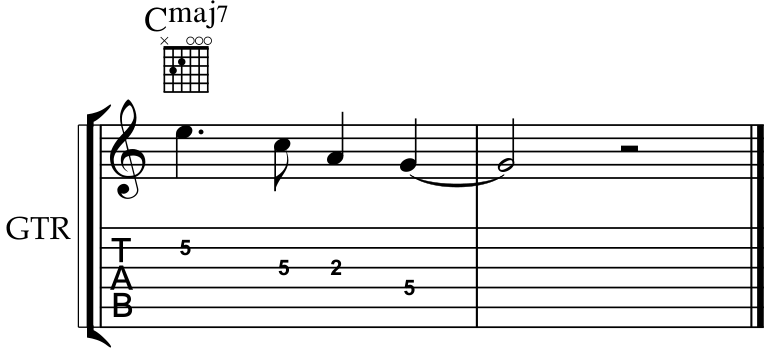
\includegraphics[width=.6\textwidth]{images/chapter2/guitarnotation.png}
            \captionsetup{width=.5\textwidth}
            \caption{An excerpt for guitar demonstrating Boulez' three main categories of notation. From top to bottom: \textit{launching}; \textit{result}; \textit{action}.}
            \label{fig:guitarnotation}
        \end{figure}

    Per Boulez' formulation, the melody given here in traditional notation is an example of ``outcome'' notation: The pitches encoded here on the top staff represent discrete sonic events with a certain predominating frequency and a certain duration: the outcome a composer hopes to achieve. The tablature beneath serves as ``action'' notation: Numbers indicate positions on the fretboard for a particular string which will ostensibly produce the desired pitches. Finally the lead-sheet symbol above (along with accompanying fretboard diagram) are examples of ``launching'' notation: prescribing creative boundaries for improvisatory action rather than sounds themselves of the same level of specificity as the other two forms. Crucially, while any of these alone might result in a sonic outcome which would satisfy a composer, they each display a radically different level of fixity. That is to say: in this example, result notation most tightly restricts the sonic outcome, followed by action notation which, taken by itself, allows for a great deal more latitude given its lack of durational values and rests (hence its frequent accompaniment by traditional notation in transcription/pedagogical texts). Launching notation, by design, only very loosely constrains the field of potential for a performer in terms of the pitch content of the sonic result. An illustration summarizing Boulez' notation typology is given in Figure~\ref{fig:Bouleztyp}.

\begin{figure}
    \centering
    \small
    \begin{forest}
                forked edges,
                for tree={draw,align=center,edge={-latex}}
                [\textsc{Notation},circle,draw
                    [\textit{Result}
                    ]
                    [\textit{Action}
                        [\textit{Launching}]
                    ]
                ]
                \end{forest}
    \caption{Boulezian typology of music notations.}
    \label{fig:Bouleztyp}
\end{figure}
    
    Much of Boulez' lecture is concerned with factors which might lead a composer to opt for one of these forms of notation over the others. He writes:

        \begin{smallquote}
            [T]o no small degree, the desire to compose comes from the contact we have with our musical heritage, our imagination naturally---necessarily---fits itself into regions defined by the lessons we have had. We think by way of them, thanks to them; and these ideas will conform to traditional kinds of notation. Yet new methods are vital when reflection intensifies our awareness of the differences between our heritage and ourselves. Using smooth time, in the realm of duration, where pulsation is no longer evident, or any point of reference to unity, and none of the multiple units of value such unity embodies, implies that we seek out either a spatial distribution that visually represents the temporal distribution we are imagining or an approximate correspondence of values for which an exact numerical correspondence is impossible.\autocite[531]{Boulez_Nattiez_2019}
        \end{smallquote}

    \noindent For Boulez, composers typically limit themselves to traditional notation because it is only from within this traditional framework that they received their training and the bulk of their musical experiences. In essence, their musical sound/process-concepts are predominantly conceived \textit{in terms of} this notation---ergo, it represents the boundaries of their musical experience. A composer who develops a new S/PC, perhaps one which relies on a notion of spatial analogy or of some form of indeterminacy, is thus best served by a notation which traces the contours of this concept.
    
    In this way, Boulez implicitly posits a sort of smooth continuum of notational fixity spanning from hyper-precise result notation intended for machine realization (e.g. a Conlon Nancarrow player piano roll); down through the less-fixed notation for Baroque and jazz performance (featuring both a high degree of latitude \textit{and} a high degree of specificity); all the way to wide-open neo-notations (``aleatoric music [...] `floating' music without pulsation'' or ``non-tempered intervals, where certain local notational features must be devised'') which may only specify one parameter, leaving the rest to interpretation.\autocite[53f6]{Boulez_Nattiez_2019} Interestingly, he makes no explicit mention of the now-common edge case that is the asemantic graphic score---that is, a certain type of (what I've been calling) ``image-first'' score---which makes no attempt to encode musical parameters at all (even while potentially gesturing at traditional glyphs, à la Cornelius Cardew's mammoth and oft-cited \textit{Treatise} 1963-7).\footnote{These asemantic works will be discussed in greater depth later in the chapter.} Neither, though, does he (directly) mention Feldmanian or Cagean graphic scores which explicitly provide keys for their interpretation. Crucially, he draws no particular distinction between these and other open notations strictly on grounds of the novelty of their encoding mechanism. 

    This wisely side-steps a problem we have not yet addressed---namely, the problem of cleanly separating what we typically think of as ``graphic'' scores from traditional or modified-traditional scores (themselves necessarily ``graphic''  insofar as they comprise written symbols as opposed to, say, strictly text). Rather, while we often categorize notations based on their appearance and the extent to which they deviate from tradition, Boulez opts to distinguish them by their \textit{function} as prescribed by either received syntax or by a composer's instructions---that is, by the way they communicate. Action, result, or launching notations might take familiar or unfamiliar forms, but in the end it is their syntax and communicative semantic content which differentiate them from one another rather than superficial properties of their physical traces.

    In the end (perhaps unsurprisingly) Boulez comes across as rather conservative when it comes to a composer's choice of notation; gently ribbing those who spring at the chance to devise radical new systems seemingly for their own sake.

    \begin{smallquote}
        With new objects [...] whose codes are presently uncertain, even non-existent, transcription becomes difficult, imprecise [...] complex to the point of uselessness[...] The problem lies in the attention required by the signs defining the object that one wants to communicate -- quantitative or qualitative. Familiar signs, newly invented signs, super-elaborate signs, deceptive signs -- a large number of solutions are available to the \textit{inventor} who might, in time, become a composer.\autocite[532]{Boulez_Nattiez_2019}
    \end{smallquote}

    \noindent Ultimately, for Boulez, new notation ought not be conceived and adopted merely as a means to mediate or alter a performer's relationship to a musical text. Rather, innovation should always be motivated by the pursuit of greater fidelity to a composer's ``object''---i.e. her sound/process-concept. I take it, though, that in many cases composers who design bespoke notations, sometimes only encoding rather simple process concepts (``play higher than $x$,'' ``play something loud!'') are taking this mediation/alteration as their brute materials---just as Boulez took pitches and durations as his---and are thus worthy of serious consideration despite their ``inefficiency.''

    This conservatism, though, does not detract from the general salience of his argument. His analytic rubric (a) focusing on notation's function over its form and (b) permitting the smooth continuum of notation's multivariate fixity is essentially the only way forward if we take as our goal a more detailed understanding of modern notation practices. These represent a significant leap forward over Eco's binaristic take on the open work and thus is one we'll carry with us as we further assay the open music practices of the twentieth and twenty-first centuries. 



    %\begin{smallquote}
    %    *****Are the two kinds of writing compatible? Does amorphousness exclude fixity by definition, or does it confront it? The two kinds of invention, gesture and state, can indeed confront one another, corroborate each other, respond, be superimposed, in any instrumental or non-instrumental domain. They can be manipulated in such ways, but one should not forget that gesture, with all this implies regarding freedom and unpredictability, remains above all the concern of the interpreter, while state is the special domain of the machine able to realise it in better, richer and more satisfying ways. [557]
    %\end{smallquote}

    %\begin{smallquote}
    %    *****In most cases one employs a notation of action, not of outcome; this is logical, since if one desires an outcome that changes every time, it would be absurd to notate one outcome and impossible to notate all outcomes. The only adequate strategy is to describe how one is to act in terms of what materials to use; hence the dichotomy, in the notation, between the elements to be used and their mode of use. [559]
    %\end{smallquote}
    
    
%    \begin{notestuff}
%       Two important takeaways that we want to bring with us: smooth continuum of fixity and defining/categorizing/taxonomizing notations based on their functions/the relations they set up between comp/perf.
%    \end{notestuff}


\subsection{Do we need an open work?}

    Confronted with Boulez' argument, the question arises: Is it actually important that we take a stab at more robustly defining the open musical work? After all, as I concluded in a prior section, all scores performed by humans are at least trivially ``open'' insofar as they all permit (demand) some degree of conscious or unconscious creative decision-making on the part of a performer before the work is able to exist---as intended---as sonic products. Each symbol, no matter how strict, merely affords a field of potential action to a player and will always contain far more than one relevant gesture; ergo, the product is not strictly regulated pre-performance; ergo it is open. Ultimately, though, this leaves us unsatisfied. Ask a pianist who has played both \textit{Structures I} and Brown's \textit{December 1952} which piece (if either) is open and which (if either) is closed. Ten times of ten they'll respond that the latter is---or at least feels---wide open. I take it that a robust notion of open works must be able to account for this experiential discrepancy; that is, it must be able to point to the most salient features of the composer/score/performer relationship which bring about this phenomenological difference.
    
    The simplest solution would be to claim that a score is open if its symbols denote sufficiently large (or ``broad'') fields of potential action. The breadth of this field is indeed one way we might think to class notational glyphs. After all, it is fairly clear (per Section 1 of this chapter) that \{$\vcenter{\hbox{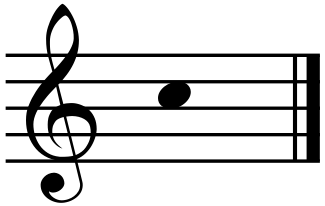
\includegraphics[width=1.2cm]{images/chapter2/c5raw.png}}}$\} affords far more potential realizations than \{$\vcenter{\hbox{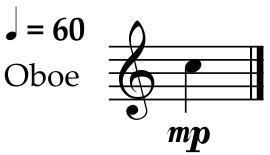
\includegraphics[width=2cm]{images/chapter2/c5oboe.png}}}$\} and thus has a broader FOP. However, it is inevitably difficult to identify, in concrete terms, magnitudes of size for these fields, given that even the ``smallest,'' most closed-off FOP permits essentially infinite realization---albeit many with vanishingly small sonic differences. Undeniably, $|FOP\{C5_{bare}\}| >> |FOP\{C5_{oboe}\}|$, but by how much? By what proportion? It remains unclear. As such, it would be untenable to categorize open works strictly according to the size of their symbols' FOP---i.e. by the sheer number of creative interpretations possible.
    
    Rather, to identify a categorical distinction characterized primarily by an \textit{experiential} difference, it would only make sense to congruently appeal to the experience of the performer. Clearly there are certain musical parameters that we as performers are accustomed to having ``held open'' in performance, despite experiencing a work as closed to creative contribution. If I, a hypothetical conservatory clarinetist, perform Stravinsky's \textit{Three Pieces for Clarinet Solo}, I experience it as a fixed work even given its inherent openness---i.e. the creative liberties afforded to an unaccompanied musician: timbre, intonation, microtiming, dynamics, etc. My experience with the piece's encoding scheme and my knowledge of the expectations which attend western concert music performance in general let me know that the larger-scale pitches, onsets, durations, and tempi are not up for negotiation and must be observed according to the score which dictates them. 
    
    When, on the other hand, I perform Louis Andriessen's \textit{Workers Union} (1975), I am suddenly presented with notation which no longer affords fixed pitches individually; or, more accurately, it affords a broad \textit{range} of pitches for each notehead present. As Boulez observed, it is often via this stripping-away of notational specificity rather than the addition of novel symbols that composers formally denote space for performer contribution. In Figure~\ref{fig:workersunion} below, Andriessen opts to encode melodic contour on a single-line staff rather than the traditional fixed-pitch five-line staff. As approximate pitch height is meant to be indicated by the relative distance from the horizontal center-line, I might begin the gesture presented at rehearsal letter \textbf{H} with a high written G$\sharp$5, A5, or A$\sharp$5, say, depending on how closely I track the spatial relationship between notehead and centerline throughout the piece.

            \begin{figure} 
            \centering
            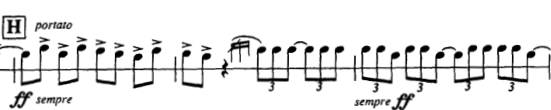
\includegraphics[width=.9\textwidth]{images/chapter2/workers_union.png}
            \captionsetup{width=.5\textwidth}
            \caption[Mm. 54-56 of Louis Andriessen's \textit{Workers Union} featuring single-line-staff notation denoting open pitches.]{Mm. 54-56 of Louis Andriessen's \textit{Workers Union} demonstrating single-line-staff open pitches.\footnotemark}
            \label{fig:workersunion}
        \end{figure}
        \footnotetext{\autocite{Andriessen_1975}}
        
    Permissible deviations in pitch have now exceeded the typical ``quantum'' unit standard notation was designed to express. Where deviations on the order of the cent are permissible (read: inevitable) from performance to performance under traditional Western classical performance conditions, Andriessen's neo-notation encodes looser constraints: repeat performances will now differ in pitch on the order of the \textit{semitone} or greater. As a clarinetist in the ensemble, the ``liberation'' of one of these typically non-negotiable musical parameters communicates to me the work's openness; striking me as an entirely new category of work. Further, while it is possible that the only noteworthy pitch deviation during Stravinsky's \textit{Three Pieces} might be my minor, unconscious shifts in intonation, at a certain level when I perform \textit{Workers Union} I must make deliberate formal commitments on the order of instrument register and specific pitch. This shifting of the domain of performance discrepancy from unconscious to conscious cognitive processes similarly renders the work ``open.'' This might explain why Berio's flute \textit{Sequenza} struck Eco as being distinct enough to include as a prime example of an open work, despite its really rather conservative affordances.\footnote{Roughly translated, its instructions read: ``The execution time and duration ratios are suggested: by the reference to a constant quantity of space which corresponds to a constant metronome beat; from the distribution of notes in relation to that constant amount of space: [empty staff showing duration of one measure at 70 M.M.]. [empty staff] is therefore equal to approximately 0.80". The [eighth-note] notes must be played free: their effective duration is suggested by the attack mode. The duration of the [multiple beamed eighth-notes] notes is intended to be extended until the next note. The value of [fermata] is ad libitum. Small notes should preferably be played as quickly as possible. The distribution ratios indicated for [fermata] and small notes are only valid as a suggestion.'' \autocite{Berio_1958}} Per Berio's instructions, onsets and durations are ``free,'' within the (fairly strict) confines designated by the given spatial proportions. This liberty is enough, though, to demand willful creative contribution from the player and ultimately to produce variances which exceed the typical discrepancy between theoretical and observed expressive attack timings (often much less than the duration of a sixteenth note); thus it strikes the player as a new sort of freedom.\autocite{Benadon_2009}

    In sum, the best way to go about arguing for a distinct category of ``open'' musical works is to appeal not to composer desires, nor the physical trace of the score, nor even to the sheer number of potential unique realizations, but instead to the phenomenal qualities of the performer's engagement with the work. If, by dint of the player's active decisionmaking, willful creativity, surprise, etc., she feels as though she's engaged with a new type of work distinct from the sometimes typewriterly experience of more traditional ``fully-notated'' music; then the work is an open one.
    
    In the end, though, there are enough edge-cases to render the initial question moot. The score for James Tenney's \textit{Having Never Written a Note for Percussion} (1971) consists entirely of one single-line staff for any percussion instrument; featuring no tempo indication, no time or key signature, and only a single rolled whole note centered on the notecard-sized page (see Fig.~\ref{fig:tenney}). 

            \begin{figure} 
            \centering
            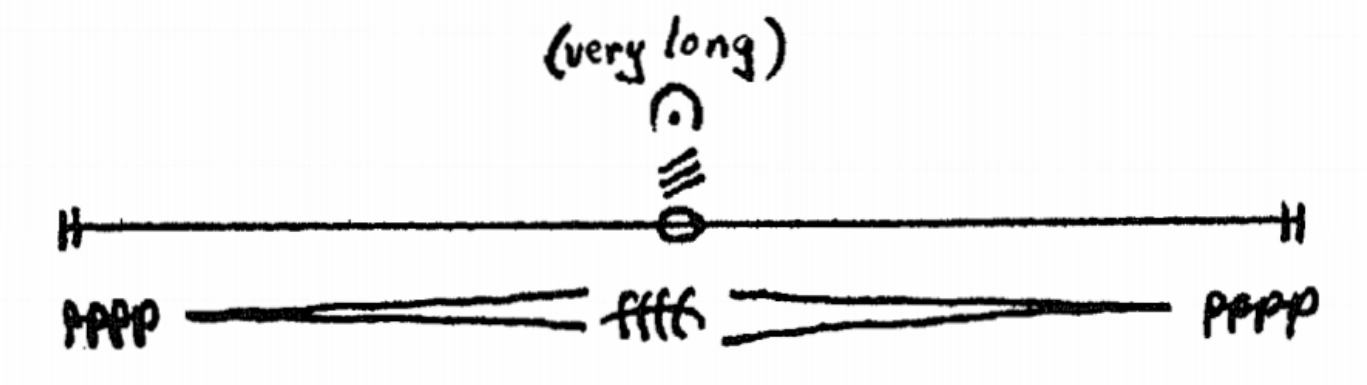
\includegraphics[width=.8\textwidth]{images/chapter2/tenney.png}
            \captionsetup{width=.5\textwidth}
            \caption[Full score of James Tenney's \textit{Having Never Written a Note for Percussion.}]{Full score of James Tenney's \textit{Having Never Written a Note for Percussion.}\footnotemark}
            \label{fig:tenney}
        \end{figure}
        \footnotetext{\autocite{Tenney_1971}}

    \noindent Performance consists of a single swell from \textbf{\textit{pppp}} to \textbf{\textit{ffff}} and back---to be played over a ``very long'' period. The total performance duration is entirely up to the performer: a small sampling of YouTube performances range from one minute to thirty. Though it is most often performed on the largest gong one can muster, any percussion instrument may be selected. Given that the whole note is of uncertain duration, the three-line tremolo indication (typically representing either an unmeasured or a thirty-second-note roll for percussion instruments) is not specific with regard to frequency of attack. Clearly, this stripped-down notation conforms well to Eco's common-sense notion of open works. To the contrary, though, the piece is \textit{experienced} as solidly fixed in place. Given that the dramatic arc of the work is so structured (i.e. with a dynamic apex right at the middle), once the performer has decided upon a particular length and a particular roll frequency, she will be able to execute the work as a singular, monadic gesture; one with as little deviation from performance to performance as would arise from a wholly-traditionally-notated version of the score. Ultimately, whether we ascribe the qualifier ``open'' to the work or not, the notation affords what it affords.

    At least as pertains to deliberately-encoded structures of notation (be they of traditional, stripped-down, or novel forms) I maintain that the notion of the ``open score'' as such is a distinction without a difference; standing in for an arbitrary point on the fixity gradient. The concept may be a useful one insofar as it serves as lexical shorthand or encourages us to think more carefully about our roles as composer or performer, but it becomes increasingly obsolete in an era characterized by ever greater intermingling of compositional and improvisatory forces---both inside the classical canon and without.


%*****When deviations cross the threshold from autonomic to deliberate...
%*****For an experiential distinction, we have to appeal to experience. Musical choices made consciously \textit{feel like} independent creative contributions---ergo their associated works will feel open. 
%*****Armed with these new concepts (FOP-signification, function classification, fixity gradient) let's revisit a few of our earlier examples from Chapter 1 to formally describe what's going on between the composer/notation/performer---maybe describing things in terms of the formal descriptors I used above.
%*****As I've already discussed, it's trivially true that all human-oriented scores are ``open'' by virtue of the impossibility of identical performances. However, based strictly on the phenomenological discrepancy between performing a hypothetically ``closed'' work like a Beethoven piano sonata and an ``open'' work like Dec '52, we desire that a refined, robust definition of an open work would account for this discrepancy.

    
% \begin{notestuff}
% %**these should be accounted for by a new model of the open work.---sometime before section 2.

% %(1) what figured-bass represents and how that differs from a lead sheet symbol

% %(2) what feldman's squares represent

% %(3) what dec 1952 represents

% %(4) Is there precedent for this view? Can we read this view into existing papers even if they don't use the same neologisms?
% *** But there's a glaring problem we haven't discussed---one that is not adequately accounted-for using strictly the terminology we've been using. There seem to be two major poles in the world of neo-notational open scores: the semantic and the asemantic. Per our earlier discussion this isn't meant to be taken as a binary but a continuum---and as such we can find many works occupying all points along this gradient. While we've looked at several works along this gradient, they all share a robust grounding in representation---even Dec. 52. 
% \end{notestuff}

\section{Steps toward a typology}

%\begin{notestuff}
%    \begin{smallquote}
%        \textbf{QUESTION TWO:} The explosion of novel notation schemes in the 1950s and 1960s presented us with a new problem: that of a certain type of ``image-first’’ score—namely ones which do not purport to encode any particular musical parameters, merely laying themselves bare for interpretation by a performer in any way s/he sees fit. To what extent ought we to consider these notation at all? They certainly represent a new sort of phenomenological experience for the performer — ought we consider them an entirely new category of music representation given they don’t ``refer’’ as such to anything?
%    \end{smallquote}
%\end{notestuff}

    Thus far we have alluded to but carefully side-stepped a big issue at the heart of contemporary notation practices. At the end of the previous chapter, I compared Feldman's \textit{Projection} series with Earle Brown's \textit{December 1952} by contrasting them as representative of ``sound-first'' and ``image-first'' styles of composition, respectively. To be clear, these labels referred not to any positive attributes of the notations themselves, but to particular modes of construction favored by the composer. Where glyphs in a ``sound-first'' arrangement would be chosen for their ability to result in a specific desired sonic outcome, ``image-first'' compositions would be constructed based on a desired visual aesthetic; allowing the sounds to arise as they may.
    
    % \begin{notestuff}
    %     I may need a sentence or two clarifying this at the end of last chapter and/or at the beginning of this one.
    % \end{notestuff}
    
    It is important that this dichotomy in notation's poiesis not be confused with one which purports to say something about notation's \textit{content}. Even using the most bog-standard traditional notation, for instance (which I take it is typically used because of the particular sounds it elicits) it is quite possible to construct scores from an ``image-first'' perspective---centering the visual results. One famous fifteenth-century example is given in Fig.~\ref{fig:heart}; albeit one whose graphicality was probably never intended to impact performance per se.
    
            \begin{figure} 
                \centering
                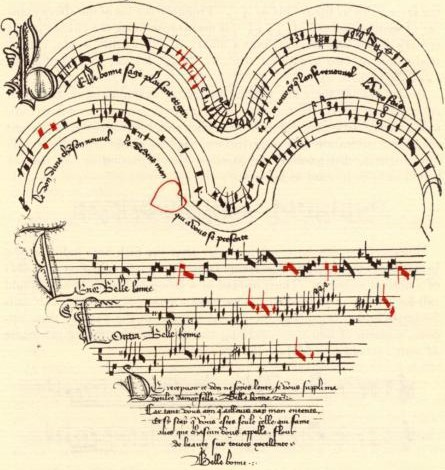
\includegraphics[width=.5\textwidth]{images/chapter2/bellebonnesage.jpg}
                \captionsetup{width=.5\textwidth}
                \caption[An early example of what might be considered ``image-first'' notation: Fifteenth-century chanson \textit{Belle, Bonne, Sage} by Baude Cordier, rendered using unconventional notation in the shape of a heart.]{An early example of ``image-first'' notation: Fifteenth-century chanson \textit{Belle, Bonne, Sage} by Baude Cordier, rendered using unconventional notation in the shape of a heart.\footnotemark}
                \label{fig:heart}
            \end{figure}
            \footnotetext{Found in the Codex Chantilly courtesy of \autocite{CHANTILLY}}
    
    \noindent On the other hand, Iannis Xenakis' electroacoustic \textit{Mycenae Alpha} (1978) (excerpted below in Figure~\ref{fig:mycenae}) is an example of ``image-first'' composition in which final sonic results are entirely contingent on the graphicality of its ``score''. Xenakis here used bespoke hardware/software to translate drawing directly into sonic contour with no performer interpretation required. What we identify as its score is really more of a complex set of computer inputs which incidentally serve as a tightly-coupled visualization.

            \begin{figure} 
                \centering
                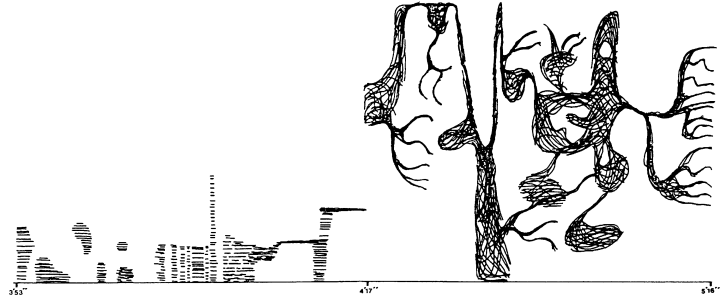
\includegraphics[width=.9\textwidth]{images/chapter2/mycenae.png}
                \captionsetup{width=.5\textwidth}
                \caption[Page 2, system 1 of Xenakis' \textit{Mycenae Alpha} (1978). Designed to be rendered precisely into sound by UPIC---bespoke visual-to-audio translation hardware/software.]{Page 2, system 1 of Xenakis' \textit{Mycenae Alpha} (1978). Designed to be rendered precisely into sound by UPIC---bespoke visual-to-audio translation hardware/software.\footnotemark}
                \label{fig:mycenae}
            \end{figure}
            \footnotetext{\autocite{Xenakis_1987}}
    
    \noindent Shifting our focus to notation's content, however, requires an entirely new formal distinction. As I hope my argument in Section 1 has demonstrated, every piece of music highlighted so far may be functionally reduced to a single type of $\text{\textit{composer}} \rightarrow \text{\textit{performer}}$ communication: a sound/process-concept is encoded for eventual transmission and execution. There exists, though, a second type of musical inscription which upends this traditional relationship by rejecting the notion that a score need necessarily encode anything at all. Neither Eco nor Boulez directly address the existence of this second type despite its consistent presence in and amongst neo-notational works since the 1940s at latest. This is not to say that their existence has gone unheeded: Many other writers have engaged with these ``asemantic'' works in one way or another, most often in the larger context of 1960s sonic indeterminacy.\footnote{For instance, Chapters 8 and 9, ``Improvisation'' and ``Indeterminacy,'' respectively in \cite{Cope_1984}; Chapter 2 ``Indeterminacy'' in \cite{Taruskin_2009d}; Chapters 2, 7, and 9 in \cite{Griffiths_2011}; etc.} Overwhelmingly, these authors fail to substantively discuss the bare function of notation and the semantic/asemantic distinction among these scores; grouping these types together under categories like ``improvisatory works,'' ``indeterminate works,'' ``aleatoric works,'' etc. Descriptors like these purport to say something about the composer's attitude toward openness, the relationship between composer and performer, and/or their desire for sonic indeterminacy---topics which of course merit discussion on their own. However, distinctions like these universally fall short of probing the actual mechanics of the works' fundamental building blocks: their inscriptions and their signs.

    Thus far my survey of relevant literature has focused on well-known and widely-published scholarship. However, by far the most thoughtful and comprehensive treatment of the taxonomy and function of new notations comes in the form of György Ligeti's little-known essay \selectlanguage{german} \glqq Neue Notation---Kommunikationsmittel oder Selbstweck?\grqq \selectlanguage{english} (``New Notation---Means of Communication or an End in Itself?'') published in a special 1965 issue of the Darmstadt journal of new music.\footnote{I'd like to extend an extra special ``thank you'' to Dr. Amy Bauer for providing a provisional translation of this paper. Coincidentally, it received its first official translation into English just as I began fleshing out this chapter. It is this translation which I will cite throughout this section, though given that it has no official page numbers, I'll cite page numbers as they appear in the original German-language edition. Original paper found in \autocite{Ligeti_1965}} Given that no extant English-language scholarship discusses this fascinating article, I would like to dedicate the following section to a thorough unpacking of Ligeti's insights; extending to both this important functional dichotomy and to aspects of notation already addressed in some detail in this chapter.

    \subsection{``New Notation---Means of Communication or an End in Itself?''}

    Vis-à-vis the article's title, the main thrust of Ligeti's argument is that depending on the precise way it is deployed, a novel system of musical notation may serve either as a means of communicating desired sound-concepts from a composer to a performer, or as a standalone performance-stimulating work of art, or both. Composers make decisions about how best to represent the ultimate sonic trace of the work depending on their artistic aims. However, Ligeti, unlike many other scholars, takes great pains to differentiate systems of notation proper from what he dubs ``musical graphics''. Not to be confused with the more common usage of the term ``graphic notation,'' which we often take to mean anything distinct from traditional staff-dot-stem-beam notation, Ligeti's use of the term here parallels what I have so far called ``asemantic'' notation---i.e. deliberately un-coded.
    
    These graphics, he claims, bear the same relationship to a composition's sonic products as a drawing of a house does to the actual, three-dimensional house it represents. The drawing does not ``mean'' the house---it merely serves as a depiction; allowing one to recognize the really-existing structure in its two-dimensional contours, but not to construct the house by following detailed instructions.  This depiction (of the sound or of the house) does not rise to the level of a sign in that it does not stand in a logically consistent network alongside other graphic depictions. 

    We might once again take Cardew's \textit{Treatise} as an example (minimally excerpted below in Figure~\ref{fig:Treatise1}):

            \begin{figure} 
                \centering
                \fbox{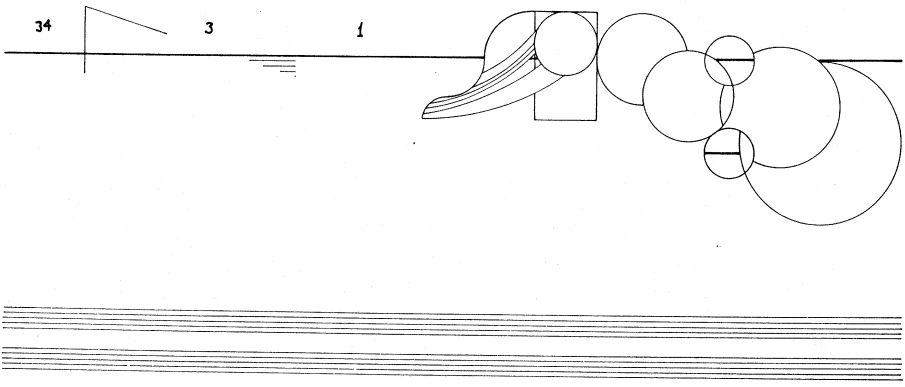
\includegraphics[width=.9\textwidth]{images/chapter2/cardewtreatisepg1.png}}
                \captionsetup{width=.5\textwidth}
                \caption[First page of Cornelius Cardew's asemantic magnum opus, \textit{Treatise}(1967).]{First page of Cornelius Cardew's asemantic magnum opus, \textit{Treatise} (1967).\footnotemark}
                \label{fig:Treatise1}
            \end{figure}
            \footnotetext{\autocite{Cardew_1967}}

    \noindent Famously, despite an enigmatic gesturing toward traditional notation in the form of the clefless grand staff at the bottom of the page, the ``symbols'' used in the piece's construction (numbers, line segments, overlapping circles, etc.) bear no composer-mapped semantic content. Construction of meaning is left entirely as an exercise to the interpreter. Insofar as one particular inscription can not be said to stand in any particular relationship to any other (save spatially), Ligeti takes these sorts of scores as comprising not notation, but something wholly separate.

    For Ligeti, notation proper\footnote{To avoid confusion, I'll use ``notation proper'' to refer to Ligeti's understanding of the term; distinguishing it from common usage.} necessarily forms an internally coherent system unto itself whose inner relationships bear some resemblance to the system of relationships present in the final sonic object---a system wherein notational glyphs (serving as signs) are laden with semantic content and which ``[correspond] to a system of auditory processes'' rather than standing in for sound directly.\autocite[pg. 171 in Ernst et al., 1965.]{Ligeti_forthcoming} He emphasizes that a means of scoring may only be dubbed ``notation'' so long as some means of inter-translatability exists between it and another coherent system of signs. Just as we could freely translate between (to use his example) FORTRAN and programmers' punch cards, so may we translate between traditional notation and, say, the ``piano roll'' notation used in digital audio workstations. Attempting to translate an asemantic graphic score in the same way would inevitably result in failure, Ligeti claims; thus it can't be considered notation at all but a wholly distinct type of composition. Over the course of the following section, Ligeti goes on to establish a tentative typology; one which seeks to encompass every form of what we might generally call ``music inscriptions,'' focusing primarily on breaking down the many varieties of notation proper and using several contemporary pieces as apropos case-studies. For posterity and toward the defense of my own views, I will describe this typology here.

    At the top hierarchical level sit the aforementioned ``notation'' and ``graphics,'' cleanly separated by their contents: coherent relations with other signs on one side and pictorial marks on the other. Notation is divided into  two primary categories: what he calls ``result notation'' (\textit{Resultatnotation}) and ``realization notation'' (\textit{Realisationsnotation}).\footnote{Notably similar to but distinct from Boulez' own categories.} Result notation is by far the most deterministic. So dubbed because it is ultimately the sonic result which is depicted on the page, result notation is used when uncertainty between the scored ``map'' and the final sonic ``territory'' ought to be kept to a minimum. Most traditional notation, for instance, falls into this category. As it is typically deployed, a transcription can result in a near one-to-one mapping between image and sound. Result notation is also used in scored electronic music where frequencies, durations, linear/nonlinear movement, etc. have been mapped with exacting precision graphically. Here, Ligeti cites an excerpt from Friedrich Cerha's ``Mouvement II'' from \textit{Mouvements I-III} which precisely represents moment-to-moment changes in pitch using glissando curves---accurately visually mapping the frequency content present for each instrument.

    % \begin{notestuff}
    %    If I decide to keep Boulez, I need a paragraph or so contrasting Boulez' language to Ligeti's---and noting his lack of attribution.
    % \end{notestuff}

    Realization notation\footnote{...which, confusingly, Boulez would later refer to as ``action notation''...} serves instead as guidelines for actions which, if successfully performed will ``realize'' the desired sonic output. Realization notations ``may be totally clear, partly clear, or unclear,'' depending on the practical needs of the composer and the desired level of fidelity between the score and product. As realization notations become increasingly complex and precise, Ligeti claims, they begin to approach result notation in the tightness of their coupling to resultant sound.\autocite[pg. 178 in Ernst et al., 1965.]{Ligeti_forthcoming}

    This realization notation is itself further divided into two categories---``action notation'' (\textit{Aktionsnotation}) and ``recipe-'' or ``formula notation'' (\textit{Rezeptnotation}). Recipe notation is perhaps easier to grasp, occurring when a composer lays out perfectly clear step-by-step instructions describing what the performer must do to achieve a desired sound. This notation is often formulated as textual instructions (e.g. ``softly strike a twelve-inch diameter tom-tom at the two-o'clock position one inch from the rim three times quickly'') but also includes tablature notations which (as mentioned earlier in the chapter) describe the precise positioning of the hands and fingers necessary to sound as the composer intends. Recipe notation, unlike result notation, bears no direct parallels to the resultant sound. Instead, it is deployed in scenarios where (a) multiple paths exist which would result in a desired sound (and the composer seeks to isolate a single path for the performer) or (b) where notating the performer's step-by-step movement is ultimately more economical than encoding the resulting sound; notating the twist of a knob, for example, rather than the complex sonic output of a synthesizer.

    Action notation, on the other hand, is on balance the least deterministic of the group. Like formula notation, it too exists to demonstrate a space of action to a performer which will result in a given sound or range of sounds when physically emulated. However, rather than providing a clear step-by-step recipe, it illustrates a visual analogy that the performer must interpret. Ligeti here cites the non-deterministic notation for the organ (which many others would incorrectly class as ``graphic'') found in Mauricio Kagel's 1972 \textit{Improvisation ajoutée} (Fig.~\ref{fig:kagel1}). 

        \begin{figure} 
        \centering
        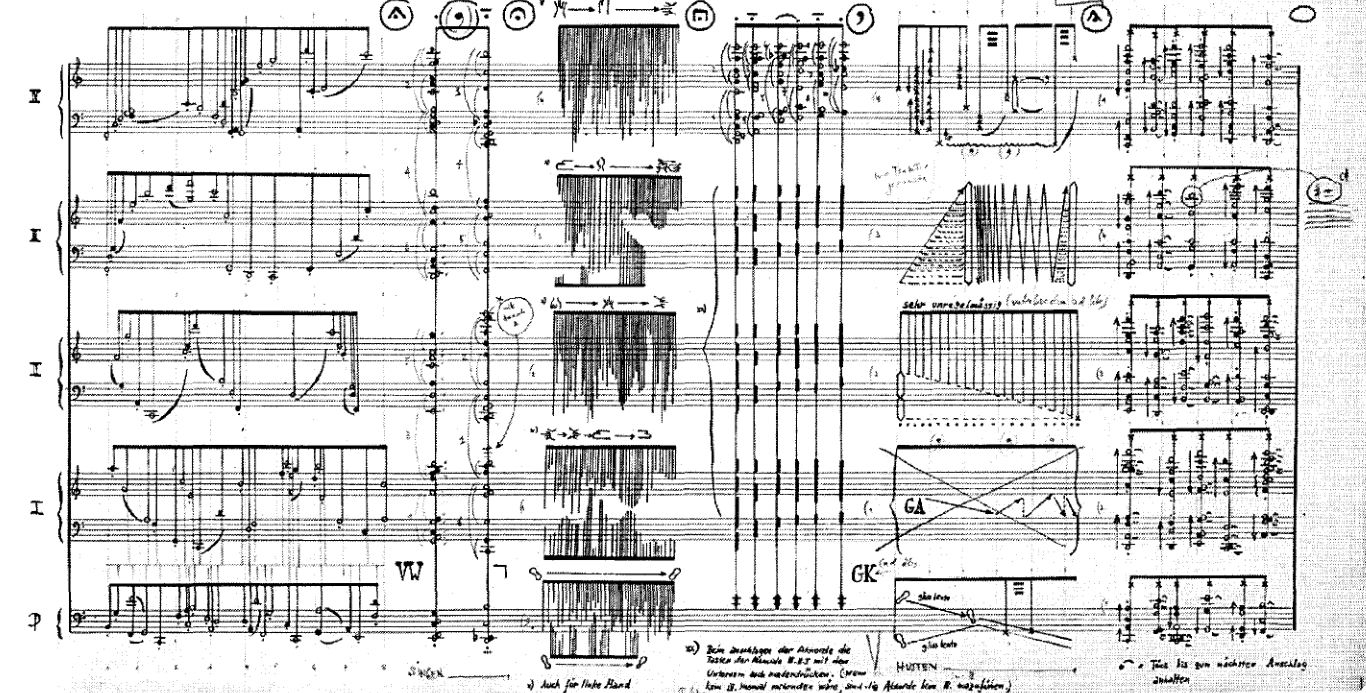
\includegraphics[width=1\textwidth]{images/chapter2/kagel1.png}
        \captionsetup{width=.5\textwidth}
        \caption[Excerpt of Mauricio Kagel's \textit{Improvisation ajoutée} (1972) courtesy of Ligeti's original paper.]{Excerpt of Mauricio Kagel's \textit{Improvisation ajoutée} (1972) courtesy of Ligeti's original paper.\footnotemark}
        \label{fig:kagel1}
    \end{figure}
        \footnotetext{\autocite[181]{Ligeti_1965}}

    Here we find glyphs seemingly based on traditional stems and beams, but impossibly tightly-packed into such a small space that a performer could not be reasonably expected to execute their attacks with a traditional level of ``faithfulness'' to the sign. Thus the performer must directly analogize their own physical gestures with the visual representation shown on the staff---the result being necessarily less precise than the sonic output of a result notation. Below in Figure~\ref{fig:Ligtyp} I've provided a tree diagram summarizing the above description of Ligeti's hierarchy of notation types (contrast with Figure~\ref{fig:Bouleztyp} above).

\begin{figure}
    \centering
    \small
    \begin{forest}
                forked edges,
                for tree={parent anchor=south, child anchor=north,draw,align=center,edge={-latex}}
                [{\textsc{Inscription}},circle,draw
                 [Notation\\(proper)
                    [{\textit{Result}}, tier=word
                    ]
                    [{\textit{Realization}}
                        [{\textit{Action}},tier=word
                        ]
                        [{\textit{Recipe}},tier=word
                        ]
                    ]
                ]
                 [{Graphic},tier=word
                 ]
                ]
                \end{forest}
    \caption{Ligetian typology of music notations.}
    \label{fig:Ligtyp}
\end{figure}

 Crucially, his rendering includes space for signs and systems which do not conveniently fall into one of the above categories---without which, any attempt to theorize notation would be woefully incomplete. Ligeti describes ``intermediate forms'' which demonstrate attributes of both symbolic notation and musical graphics, of which Brown's \textit{December 1952} is his prime example.\footnote{It seems here that Ligeti, like Griffiths, was under the mistaken impression that \textit{December 1952} lacked any preambulatory text or instructions. His argument is based on this assumption and thus treats the work like a particularly well-structured ``graphic'' rather than a notation as such. We'll bracket this oversight for now, as it doesn't particularly impact the thrust of his argument.} Ligeti interprets Brown's work as both a graphical work unto itself as well as a formally delimiting agent; setting distinct (though imprecise) boundaries for performer interpretation via its visual arrangement. Ligeti claims:

\begin{smallquote}
    If [\textit{December 1952}] is realized musically, there are numerous possibilities---and yet the interpretation is not totally free, because the visual configuration sets quite definite limits. In this regard, this musical graphic also possesses some (rudimentary) elements of a sign system.\autocite[pg. 177 in Ernst et al., 1965.]{Ligeti_forthcoming}
\end{smallquote}

\noindent Ultimately, these hybrid forms not only serve as intriguing case-studies by which we might contemplate the nature of composer/performer agency, but also lend further credence to Ligeti's typology insofar as they demand separate analysis of the function of their constituent symbolic/graphic components. ``[T]he fact that the sign component can be separated from the graphic aspect within mixed forms,'' he claims, ``is itself a demonstration that we are dealing with two fundamentally different categories.''\autocite[pg. 177 in Ernst et al., 1965.]{Ligeti_forthcoming}

In the end, Ligeti argues that the composer's decision to deploy either a system of (neo-) notation or a pseudosystem of musical graphics rests on a question of desired ``adequacy, clarity, and economy'' in musical representation. His thesis here relies on a vivid analogy which takes the purely graphic score to be the \textit{map} of a particular (sonic) territory and the notated score to be the walking of a \textit{single path} through that territory. The musical graphic is both richer and more ``wasteful'' in that, like the map, it contains innumerable details pertaining to countless ``hikes'' that cannot be experienced in a single journey. In the act of performative interpretation, one necessarily discards every unrealized detail in favor of the chosen path. The ``single walk,'' on the other hand, has its own inner richness in that it is able to reveal features invisible on the map---foregoing potential variety of experience for finer-grained detail and ``paripeteias'' otherwise inaccessible to such a zoomed-out view. The decision to enlist either the map or the path thus rests on the extent to which a composer seeks reproducibility and fine-grainedness or the richness of unlimited, irreproducible detail.\autocite[pg. 178 in Ernst et al., 1965.]{Ligeti_forthcoming}

Because, Ligeti  claims, scored instrumental and vocal music always retains some ``margin of vagueness'' when contrasted with fixed electronic music, and because this vagueness is always already intimately tied up with the notational markings used to represent a flexible, imprecise music, systems of notation will tend to reflect this flexibility and imprecision. Thus, as contemporary composition varies wildly in its degree of determinism from piece to piece (and even within pieces!), pure one-size-fits-all systems of notation tend to be eschewed in favor of meta-systems which hybridize characteristics from pure graphics, result notation, action notation, and recipe notation depending on the particulars of the composition in question. The notation used to encode Kagel's \textit{Improvisation ajoutée}, per Ligeti's example, succeeds not because it attempts to be unified and all-encompassing, but precisely because of the extent to which it hybridizes notations spanning Ligeti's typology: result notation in the form of determinate pitches, action notation for the organists hands and feet, and formula notation for entabulating the organ's stops.\autocite[pg. 180 in Ernst et al., 1965.]{Ligeti_forthcoming}

% \begin{notestuff}
%     Boulez' complaint from earlier about the prevalence of bespoke, non-standardized solutions could be seen to be in response to this mashing together of different notation schemes without a sort of meta-theory guiding their use.
% \end{notestuff}

\subsection{Why are Ligeti's typology and analysis valuable to us today?}

Ligeti's appraisal of the structure and use of these distinct forms of notation and graphics, perhaps owing to his practical, composerly experience with many of these forms, is strikingly refined in contrast to other historical and contemporary takes on the matter. As such, I take it that further elucidation of this typology might be of some use in the study of notation and of ``open'' composition today. Ligeti is one of only a few scholars to draw a firm distinction between methods of music inscription on grounds of their semantic content or lack thereof---that is, on whether they denote concrete musical materials or merely connote potential spaces of action. Where many authors ambiguate these two antipodean categories under the label ``graphic notation,'' ``indeterminate notation,'' etc., for Ligeti, the fundamental property of an inscription is not its novelty, but its contents.

Under Ligeti's formulation, the fixity of a notational glyph or set of glyphs does not necessarily correlate one-to-one with the strength of its semantic content. A functional, logically coherent sign system may have highly-fixed sounds or gestures as its points of reference, as in the precisely-engraved result notation of a piece of electronic music. On the other hand, a similarly coherent, denotative notation may point to highly \textit{indeterminate} sounds or gestures---for instance, the dense, headless grace-note figures from \textit{Improvisation ajoutée} or Feldman's pitch-range notation. These figures are notational rather than graphic in the sense that while the performer's creative act of reading will vary significantly from performance to performance, the composer had a key role in determining the bounds of that semantic content (and therefore in predictably influencing the sonic products resulting from the figures' realization).

As such, Ligeti separates notation's relative fixity or openness from its ability to meaningfully communicate. One might imagine a less nuanced view, whereby a glyph's communicative potential is strictly proportional to the quantity of its fixed content. A mode of inscription totally lacking sonic specificity would thus be unable to effectively communicate anything at all. Given, though, that many such sonically indeterminate works (including wholly asemantic works) enjoy repeat performances and some form of persistent identity, we should prefer to say that they retain  communicative potential, despite their irreducibility to one particular sound world. We might represent these opposing univariate and bivariate views using ``denotative'' to indicate the presence of composer-provided semantic content and ``connotative'' to indicate its absence (Fig.~\ref{fig:typologies}).

\begin{figure}
    \centering
            \begin{tabular}{ |c|c| }
             \hline
             \multicolumn{2}{|c|}{\textbf{Traditional univariate typology}} \\
             \hline
             fixed and denotative & open and connotative  \\ 
             \hline
            \end{tabular}

                \vspace{10pt}

            \begin{tabular}{ |c|c| }
             \hline
             \multicolumn{2}{|c|}{\textbf{Ligetian bivariate typology}} \\
             \hline
             fixed denotative & \textcolor{gray}{fixed connotative\footnotemark}  \\ 
             \hline
             open denotative & open connotative  \\     
             \hline
            \end{tabular}
    \caption{Univariate vs. bivariate notation typologies.}
        \label{fig:typologies}
    \end{figure}
            \footnotetext{``Fixed connotative" notation is a category merely implied by the existence of its antitheses. This is as-yet untheorized as it would require a notation which is somehow ``defined" by its interpreter but which is nonetheless semantically stable across performance scenarios. The lack of a well-defined ``fixed connotative" notation forces me to refer to fixity and content as only ``quasi-independent" rather than truly independent properties.}

    \noindent While under the old view, notation's content is directly proportional to its fixity, only concretely denoting insofar as its sonic products are predictable, under Ligeti's new bivariate view, notation may strongly denote regardless of the indeterminacy of its products.

    To elaborate on this distinction: Here, ``fixed denotative'' notation describes that which has been rendered systematic ahead-of-time by the composer or by received practice. The final sonic trace of the work is more-or-less predictable/replicable because the notation hews closely to the final sonic product. Note that this is to say nothing of how closely it resembles traditional notation in its printed form; traditional notation does indeed fit into this category---but so does, say, the widely-adopted ``cipher'' tablature commonly used to notate Indonesian gamelan compositions (Fig.~\ref{fig:gamelannot}).

    \begin{figure}
        \centering
        \fbox{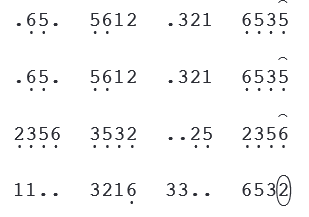
\includegraphics[width=.4\textwidth]{images/chapter2/gamelancipher}}
        \captionsetup{width=.5\textwidth}
        \caption[\textit{Nut angka} contemporary style of gamelan notation demonstrating an excerpt of \textit{Gending Titipati sléndro pathet nem}.]{\textit{Nut angka} contemporary style of gamelan notation demonstrating an excerpt of \textit{Gending Titipati sléndro pathet nem}.\footnotemark}
        \label{fig:gamelannot}
    \end{figure}
        \footnotetext{\autocite{Ishida_2008}}

    \noindent The ``open connotative'' type, on the other hand, describes what Ligeti calls musical graphics---asemantic drawings which have no ahead-of-time systematicity. These figures only have meaning insofar as it is given by the interpreter, either pre-performance or in-the-moment (hence connotative). The quasi-symbols depicted on the page merely ``suggest'' musical moves; the final sonic products are entirely downstream of the performer's decision to (or refusal to) map glyphs to gestures themselves.
    
    %The formal distinction between ``open connotative'' and ``open denotative'' notation represents a significant point of refinement for Ligeti's view over those of his peers.
    
    Finally, the ``open denotative'' category refers to the structures of notation that have thus far been the primary topic of this study---specifically those in which symbols explicitly encode desired fields of potential action, but deliberately leave space for willful creative interpretation on the part of the performer. In other words, they bear semantic content (hence denotative) but maintain an indeterminate sonic trace. Per Section 1, the particular quality and quantity of semantic ``data'' they bear is merely a function of the specificity with which it shapes the field of potential action afforded to a performer. 

    Where Figure~\ref{fig:Ligtyp} demonstrated Ligeti's typology as expressly relayed in his article, Figure~\ref{fig:Amendtyp} below refines this typology by making explicit the implied categories of semantic-fixed and semantic-open notations (again, distinct from asemantic, connotative notations). Note that, per earlier discussion, these categories do not represent a hard binary but rather two poles delineating a smooth gradient.

    \begin{figure}
    \centering
    \small
    \singlespacing
    \begin{forest}
                forked edges,
                for tree={parent anchor=south, child anchor=north,draw,align=center,edge={-latex}}
                [\textsc{Notation},circle,draw
                 [{\textbf{Denotative}}
                    [{Semantic\\fixed}, name=A
                        [{\textit{F. Res.}},tier=word]
                        [{\textit{F. Real.}}
                            [{\textit{F. Act.}},tier=word]
                            [{\textit{F. Rec.}},tier=word]
                        ]
                    ]
                    [{Semantic\\open}, name=B
                        [{\textit{O. Res.}},tier=word]
                            [{\textit{O. Real.}}
                                [{\textit{O. Act.}},tier=word]
                                [{\textit{O. Rec.}},tier=word]
                            ]
                    ]
                ]
                 [{\textbf{Connotative}}
                    [{Asemantic\\open},tier=word]
                 ]
                ]
                \draw[<->,dotted] (A)  to[out=east,in=west] (B);
                \end{forest}
    \captionsetup{width=.5\textwidth}
    \caption{Refined Ligetian typology of music notations. Dotted arrow indicates presence of ``fixity gradient'' between the semantically fixed and open genera.}
    \label{fig:Amendtyp}
\end{figure}
    
    %For Ligeti, notations proper are divisible into his distinct subcategories (result, action, recipe) only because of their ability to properly encode and transmit composerly intent. The strictly connotative ``graphics'' on the other hand are essentially brute fact---differentiable only by the qualities of their inscription.

    Among Ligeti's many observations, the relatively intuitive division of musical inscription into two fundamental categories---the semantic/denotative and the asemantic/connotative---represents a significant point of refinement for typologies of notation in general. I take it that this (in conjunction with his subcategories of notation proper) permits a more nuanced understanding of mid-century sonically-indeterminate notations and their descendants than is typical of the field. Let us take, for example, two works from the same time period which make extensive use of neo-notation: John Cage's \textit{Concert for Piano and Orchestra} (1957-8) (see Fig.~\ref{fig:cagepiano1}) and No. 1 from Sylvano Bussotti's \textit{Five Piano Pieces for David Tudor} (see Fig.~\ref{fig:bussottipiano1}). 

    \begin{figure}
        \centering
        \fbox{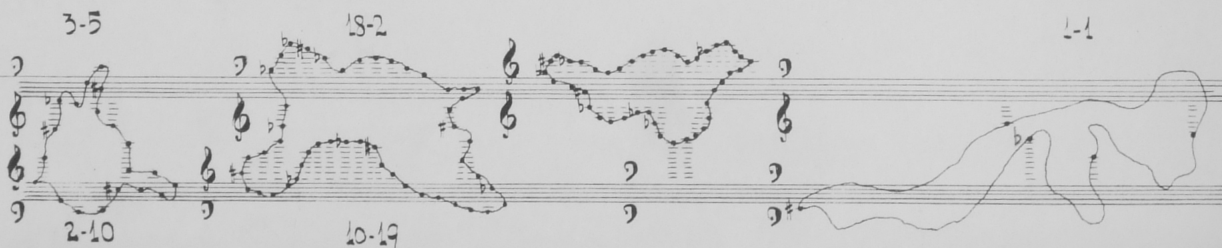
\includegraphics[width=.99\textwidth]{images/chapter2/cagepianomoduleL.png}}
        
            \vspace{10pt}
            
        \fbox{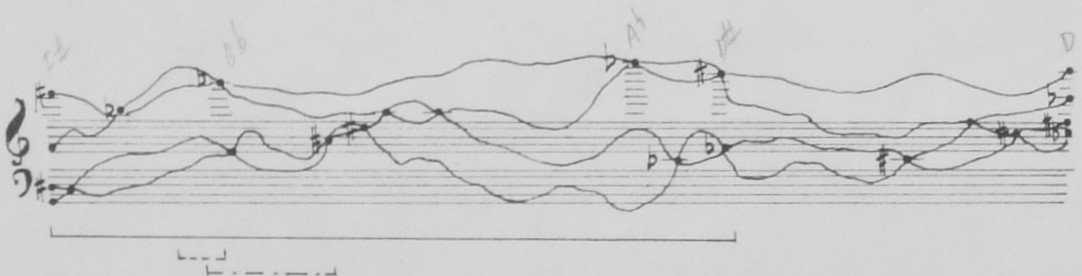
\includegraphics[width=.99\textwidth]{images/chapter2/cagepianomoduleM.png}}
        \captionsetup{width=.5\textwidth}
        \caption[Modules ``L'' and ``M'' from the piano solo of Cage's \textit{Concert for Piano and Orchestra} (1957-8).]{Modules ``L'' and ``M'' from Cage's \textit{Concert for Piano and Orchestra} (1957-8).\footnotemark}
        \label{fig:cagepiano1}
    \end{figure}
        \footnotetext{\autocite{Cage_1960}}

    \begin{figure}
        \centering
        \fbox{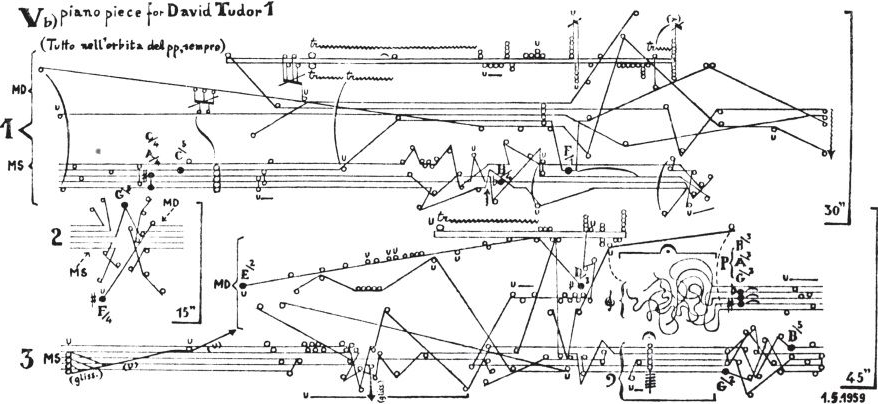
\includegraphics[width=.99\textwidth]{images/chapter2/BussottiPiece1.png}}
        \captionsetup{width=.5\textwidth}
        \caption[Full score of No. 1 from Sylvano Bussotti's \textit{Five Piano Pieces for David Tudor} (1959).]{Full score of No. 1 from Sylvano Bussotti's \textit{Five Piano Pieces for David Tudor} (1959).\footnotemark}
        \label{fig:bussottipiano1}
    \end{figure}
        \footnotetext{\autocite{Bussotti_1959}}

        At first blush, there are many commonalities between these two excerpts. Both are pieces for unaccompanied piano which ground the performer in their sense of musical literacy by using familiar glyphs: staves, clefs, points which might represent attacks, linear or curved connectors. Both are clearly sonically indeterminate; requiring a significant degree of creative interpretation for their realization. The critical distinction between the two is that while Cage's piano solo came packaged with detailed instructions defining the boundaries of successful interpretation (excerpted below for context)...

    \begin{smallquote}
        \noindent \textsc{[...] the whole is to be taken as a body of material presentable at any point between minimum (nothing played) and maximum (everything played), both horizontally and vertically [...]}
    \end{smallquote}
        \vspace{-20pt}
    \begin{smallquote}
        \noindent \lettrine[lines=2, findent=3pt, nindent=0pt]{B}{:} \textsc{[...] the single staff is provided with 2 clef signs. where these differ, ambiguity obtains in the proportion indicated by the 2 numbers above the aggregate, the first of these applying to the clef sign above the staff.} [...]
    \end{smallquote}
        \vspace{-20pt}
    \begin{smallquote}
        \noindent \lettrine[lines=2, findent=3pt, nindent=0pt]{L}{:} \textsc{play from left to right with hands indicated. clef ambiguity as in B. perimeters were composing means and do not here affect time, as they do in a.}        
    \end{smallquote}
        \vspace{-20pt}
    \begin{smallquote}
        \noindent \lettrine[lines=2, findent=3pt, nindent=0pt]{M}{:} \textsc{begin at left, end at right, changing direction at intersections if desired. may be expressed as one voice, a `counterpoint,' or as 3 or 4 voices. pedals only in areas indicated, not obligatory.}\autocite[pg. B]{Cage_1960}
    \end{smallquote}




    \noindent ...Bussotti's instructions for his piece for Tudor begin and end with the Italian inscription at the top of the page: ``All in the orbit of \textbf{\textit{pp}}, always.'' 
    
    While Cage's work inarguably compels a performer to interpret its symbols creatively, it does so by restricting (with lesser or greater degrees of rigor) the performer's field of potential using the symbols' semantic content which Cage himself encoded. To use Ligeti's terminology: the floating noteheads are examples of result notation in that they ought to result in the sounding of particular pitches.  The ``aggregates'' of which they are members, though, are forms of action notation in that they provide a visual/spatial analogy for onset/duration to which the performer must hew. The text block preceding the piece is a sort of recipe notation insofar as it expressly denotes conditions for successful interpretation. Bussotti's work, on the other hand, predominantly comprises Ligetian ``musical graphics'' in that (beyond the initial inscription) the piece relies \textit{entirely} on performer interpretation. Its familiar appearance and sprinkling of recognizable glyphs belie the fact that Bussotti intended the work in its entirety to serve as ``launching'' notation (to use Boulez' term); essentially in contravention of all received notions of musical literacy. Bracketing the \textit{pianissimo} indication, any constraint on the potential action of the performer is up to the performer herself.

    Many authors expressly or implicitly make the case that Cage and Bussotti's works from this period represent two adjacent ideological camps with regard to performer liberation---both employing a similar compositional language with Bussotti merely taking the marginally more ``radical'' tack in his permissiveness. What Ligeti illuminates, however, is that owing to their semantic structures, these two inscriptions represent two entirely distinct classes of ``writing,'' with appropriately distinct structures of agency. Both are ``graphic'' in the colloquial sense of the term in that they depart from standard music encoding methods, but the approaches are miles apart when it comes to their actual function. Not coincidentally, Stockhausen selected works from the two series represented here when he conducted his 1959 Darmstadt lecture series entitled ``\textit{Musik und Grafik}'' (diligently analyzed by David Gutkin in \textit{Perspectives of New Music} (2012)). Though I lack the space to fully detail Stockhausen's (or Gutkin's) observations on what were then brand-new structures of notation, it's clear that both he and Gutkin take Bussotti's piano pieces to comprise a sort of implicit action notation; though one which ``only effects actions in a very indeterminate matter.''\autocite[276]{Gutkin} While they note that Bussotti's inscriptions represent a basically new compositional method, they fail to articulate that an entirely new relationship is set up between composer (here ``inscriber'') and performer---one in which essentially all \textit{restrictive} capactity belongs to the interpreter while the inscriber serves only to ``provoke'' or ``incite'' action by connotation.\footnote{Gutkin's paper is, by and large, an incisive and much-needed look at a fascinating and under-studied sector of music theory. He reads far deeper into the function and significance of strictly connotative notation than I am prepared to do here---I merely take issue with this particular characterization of Bussotti's work.} 
    
    To illustrate, I've included another interaction model (Fig.~\ref{fig:graphicdiagram}) to reflect the function of musical graphics (to contrast with that of notation proper). Noteworthy differences include: (1) The initial sound-concept becomes superfluous, the score is now merely an instance of \textit{ekphrasis}---a drawing ``about sound'' but one ultimately informed by a graphic- (rather than a sound-) concept. (2) The score merely \textit{connotes} a field of potential to the performer who (3) encounters the notation via \textit{gazing} (per Gutkin's term), producing sound which bears no necessary semantic connection to the graphic itself.

        \begin{figure} 
            \centering
            \fbox{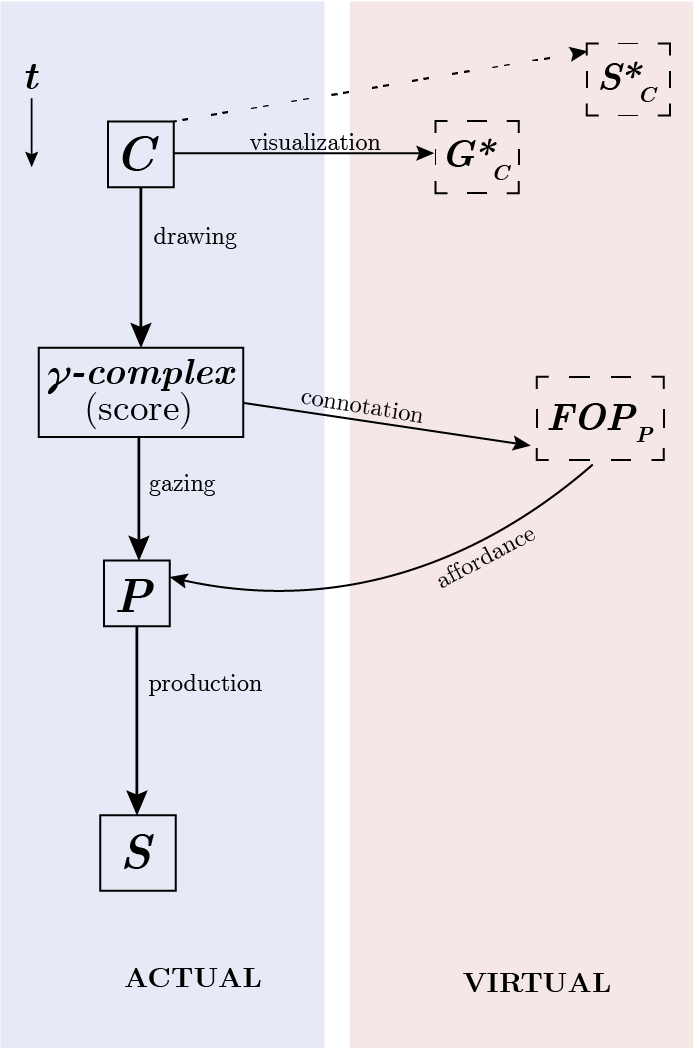
\includegraphics[width=.5\textwidth]{images/chapter2/graphic_signification_diagram.png}}
            \captionsetup{width=.5\textwidth}
            \caption{``Graphic'' interaction model---to contrast with that of notation proper.}
            \label{fig:graphicdiagram}
        \end{figure}

    As far as my interests are concerned, though, the most pertinent strength of Ligeti's typology lies in its ability to meaningfully describe ``hybrid'' works/notations---i.e. compositions which integrate, often at quite a granular level, instances of denotative and connotative notations. If we accept his analysis that semantic and asemantic inscriptions, (``sign system'' and ``illustration'') are two fundamentally distinct categories which nevertheless may ``grow into one another,'' I take it that there are two fundamental mechanisms by which this hybridization may occur.\autocite[pg. 177 in Ernst et al., 1965]{Ligeti_forthcoming}
 
    First: Over the course of a score, section of a score, or even a single gesture, a composer may employ conventionally-coded symbols (of either traditional or neo-notation) \textit{alongside} asemantic inscriptions to be freely interpreted. We might dub this style ``concatenative'' hybridity. Figure~\ref{fig:revis} illustrates one such example which I engraved for Eric Revis in 2021. Painted ``background'' portions were provided with no accompanying code and were meant to provide improvisatory grounding for the traditionally- (or mostly-traditionally-) notated floating fragments.

        \begin{figure} 
            \centering
            \fbox{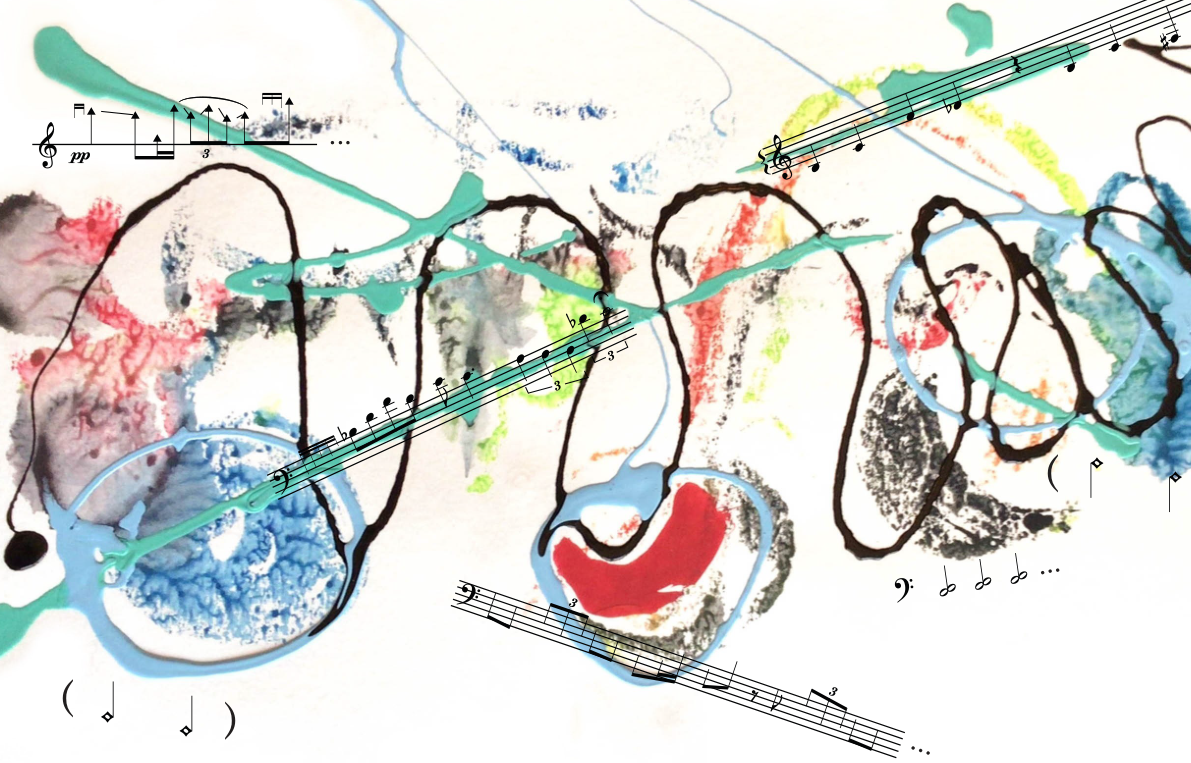
\includegraphics[width=.9\textwidth]{images/chapter2/slipknots2.png}}
            \captionsetup{width=.5\textwidth}
            \caption[Score created \textit{ex post facto} for Eric Revis' ``Slipknots Through the Looking Glass \#2'' demonstrating ``concatenative'' hybridity. Traditional and modified-traditional notations are used side-by-side with non-coding graphics.]{Score created \textit{ex post facto} for Eric Revis' ``Slipknots Through the Looking Glass \#2'' demonstrating ``concatenative'' hybridity. Traditional and modified-traditional notations are used side-by-side with non-coding graphics.\footnotemark}
            \label{fig:revis}
        \end{figure}
            \footnotetext{Original performance by Eric Revis. Painting by Ayanna Bassiouni. Transcription/engraving by Isaac Otto. Recording from \autocite{Revis_2020}.}

    Second: A single conventionally-coded symbol (either traditional or neo-notation) \textit{itself} might demonstrate noteworthy ``graphicality''---an ability to connote despite its separate, robust encoding---what we might dub ``simultaneous'' hybridity.\footnote{We might consider a third type: a semantically-coded symbol accompanied by or involving inscriptions which are strictly \textit{incidental}; neither coded to constrain a field of potential action nor designed to incite performer-mapping. It's unclear whether we ought to even consider this ``graphic excess'' notation of any sort, or whether it's best thought of as mere decoration. We might consider \textit{Belle, Bonne, Sage} shown above in Figure~\ref{fig:heart} to be an example of this third mechanism---perhaps ``decorative'' hybridity.} I take Cathy Berberian's \textit{Stripsody} (1966) (shown in Fig.~\ref{fig:stripsody1} below) to be a canonical example of this second form. Berberian provides explicit instructions for the interpretation of glyphs insofar as they conform to traditional ${time}\times{pitch}$ mapping on the $x$- and $y$-axes and standard notions of proportional duration/onset. However, each glyph (word) also demonstrates an ``excess'' of graphicality beyond simple decoration; presumably meant to influence the execution of that symbol in ways that remain un-coded. 

        \begin{figure}
            \centering
            \fbox{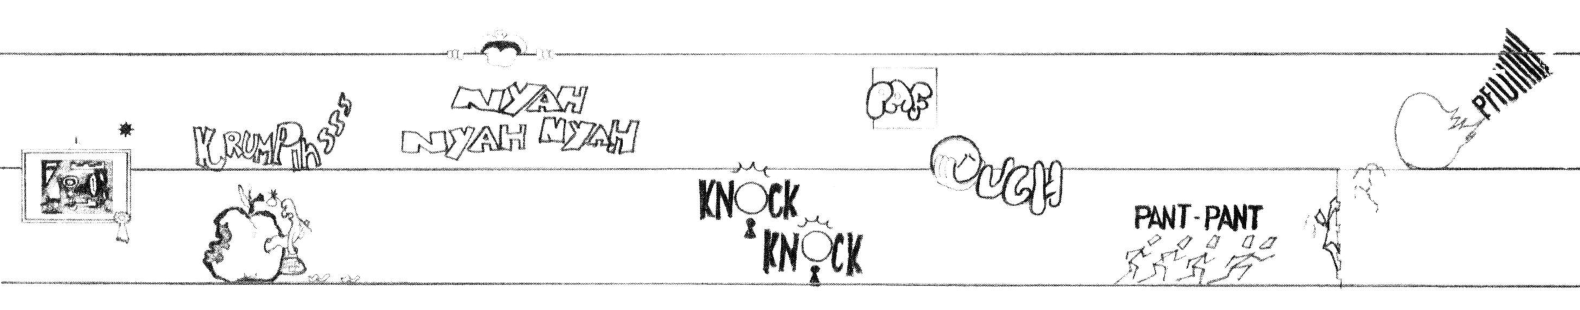
\includegraphics[width=.99\textwidth]{images/chapter2/stripsody1.png}}
            \captionsetup{width=.5\textwidth}
            \caption[System three on page four of Cathy Berberian's \textit{Stripsody} (1966) demonstrating ``simultaneous'' hybridity. Coded symbols themselves demonstrate connotative potential---i.e. ``graphicality.'']{System three on page four of Cathy Berberian's \textit{Stripsody} (1966) demonstrating ``simultaneous'' hybridity. Coded symbols themselves demonstrate connotative potential---i.e. ``graphicality.''\footnotemark}
            \label{fig:stripsody1}
        \end{figure}
             \footnotetext{\autocite{Berberian_1966}}

    Naturally, some questions remain: At what point may one claim that a notational symbol crosses over into meaningful graphicality---i.e. when does a symbol become sufficiently affective as to be able to impact performance via connotation? Precisely in which ways does this graphic excess serve to impact performance? On which factors is this graphic mediation contingent? At this point, answers to these questions would be essentially speculative, though it now seems possible to ask them empirically; in such a way that their answers might fall in the empirical domain of performance psychology and music cognition. Ultimately, I would argue that the mere ability to meaningfully raise these questions represents a new degree of subtlety in the discourse surrounding notation which would not be possible without Ligeti's analysis.


% \begin{notestuff}
%     Begin wrap-up here. Just make the claim that with the tools laid out by Ligeti and some subtle re-rendering we are much better equipped to assess what's going on in these multi-layered scores; how they work; what they afford
% \end{notestuff}
    
% \begin{notestuff}
%     *****The recognition of the existence and value of HYBRID notations I think is where a lot of the meat is. When composers (like Cage in his Concert) use deliberately evocative notations, they're in fact hybridizing two entirely different mechanisms: the restrictive and the inciting.  
% \end{notestuff}

%         \begin{notestuff}
%         \begin{center}
%         GUTKIN ARGUMENT
%         \end{center}
        
%         *****Cage and Bussotti are often discussed as two points along a continuum -- Cage still reliant on explicit instructions for the interpretation of his figures and Bussotti even more radical; allowing for any mapping desired by the performer. However these are b est understood as entirely different paradigms, which Ligeti understood! Even Stockhausen via Gutkin seems to get this wrong. These are two fundamentally different kinds of thing. These things can be HYBRIDIZED but I wouldn't call it a continuum. The mapping comes from two different places! Notation function ``flow'' chart is different! 
        
%         The vestigial notation-like glyphs on the page might provoke similar responses from performers but the fact remains that it's all performer-oriented. This is what so many seem to miss. Tudor recognized this in his transcription/performance of the Bussotti ``The piece \textit{is} the lines and the surfaces on the paper.'' (Gutkin 272)  
        
%         Signification =/= Stimulation (Gutkin 273) 
        
%         *****He's right that there's always an element of ``gazing'' in ``reading'' (pg. 277) but the reverse isn't necessarily true. No meaningful semantic communication occurs in the Bussotti and it's our responsibility to be able to differentiate these things so that we might see hybrid works as complexes of the two actions---reading and gazing.
%         \end{notestuff}

% \begin{notestuff}
%     \begin{center}
%         COPE ARGUMENT
%     \end{center}
% \begin{smallquote}
%     *****Improvisation differs from indeterminacy, as its meaning in music refers to the aspect of performer interaction, an activity more often than not controllable in rough shape by the composer, and even predictable within limits.\autocite[244]{Cope_1984}
% \end{smallquote}

%     *****Improvisation is more a notational than a philosophical challenge to tradition.\autocite[242]{Cope_1984}

%     Cope selects a bunch of open, denotative notation and works to demonstrate ``improvisation,'' but also includes William Duckworth's largely asemantic \textit{Walden Variations}. Then in his section on ``performer indeterminacy'' in the next chapter, he does precisely the same thing---including several pieces with open denotative symbols (traditional or neonotation) and then asemantic neonotation in the form of John Mizelle, Robert Moran, etc. He claims that these are notational distinctions but doesn't make an effort to differentiate the notations that characterize these two ``different'' music-making paradigms.

%     Per Ligeti's formulation, the distinction between ``improvisation'' and ``performer indeterminacy'' is strictly academic. Notated works are reducible to the function of their symbols.

%     *****Cope notes that certain pieces (bussotti) feature ``nonsymbolic abstract representation'' (282) for which ``interpretation or noninterpretation is fully within the performer's realm'' but doesn't meaningfully distinguish between these notations and those which robustly encode musical parameters. He refers to Cage's style of notation as ``somewhat graphic'' (277) without explaining what that might mean. Both of these works he categorizes as ``performer indeterminacy'' along with traditionally notated but cellular works like Stockhausen's Klavierstuck XI.
%     \end{notestuff}


    
% \begin{notestuff}
%     \begin{itemize}
%         \item Contrast with Cope's mixed-up improvisation/indeterminacy dichotomy?? At least in order to illustrate the value of Ligeti's (and my) much more performance-grounded reading of notation-mediation...
%         \item An amended notation typology    
%     \end{itemize}
% \end{notestuff}

\section{Conclusion}

To synopsize the main takeaways from the discussion presented in this chapter:

(1) It often behooves our analysis of the form and function of music notations to consider them not pictorial representations of past or potential future sounds, per se, but rather as generic coded instruction sets which denote particular mediated fields of potential musical action in performance. In order to serve as a music notation, these instruction sets must internally cohere according to a received syntax, arrived at either via the accretion of interpretive norms acquired over the course of a performer's musical education and experience, or given explicitly via the score itself.

(2) If we seek fuller understanding of the complex, multiform notations which have become more commonplace since the 1950s (and which show no sign of disappearing anytime soon!), it is important to have at our disposal a well-defined notation typology. This should address not only the graphic trace of the inscriptions used to mediate performance, but should also take into account their various mechanisms of action.

(3) Developing these definitions requires that we disabuse ourselves of certain antiquated notions surrounding the performance of scored music: namely, the notion that we might meaningfully distinguish ``open'' works from traditional ``fixed'' works. More robust definitions of extant notations should bear out that openness is a fundamental property of \textit{all} human-performed music, including music encoded using traditional methods. The more meaningful question, then, is ``In what way does this notation serve to mediate this music's openness?''

(4) As far back as the late 1950s, composers and scholars contemplated the properties, significance, and merit of new notations designed to enact sonically-indeterminate (i.e. ``open'') music. I've argued here that György Ligeti's (only recently-translated) 1965 essay stands as a valuable untapped resource demonstrating an uncommon degree of insight into these problems surrounding notation. To wit, Ligeti describes a function-oriented notation typology separating semantic notation proper from asemantic graphics. Further, notation as such is classed according to the means by which it restricts performers fields of potential action---into result, action, and recipe notations. I assert that a modified Ligetian typology provides us with a valuable new set of tools with which to assess the way notation (and other musical inscription) mediates the often complex relationship between composers, musical texts, and performers.

In the following chapter, I will use these tools to examine two late twentieth-century work-complexes by artists who have shown particular sensitivity in their use of neo-notations. These examples exist between and beyond commonly-understood notational binaries; demonstrating either deliberate ``traversal'' of the gradient between fixed and open denotative notations or poignant hybridity between the denotative and the connotative (or indeed both). 

% \begin{notestuff}
%     (There are, of course, a whole bunch of things I omitted for space---I want to at least pay lip service to them to make it clear that (some of) these omissions were intentional, but maybe I should save that for a kind of ``epilogue/future research'' bit of text after the final chapter?)
% \end{notestuff}

    % \subsection{The relative prominence of ``image-first'' or ``connotative'' scores}
    
    % \subsection{Fixity as independent variable}


% \begin{notestuff}
%     \textbf{\textit{This should go in a section of ch. 2 actually.}}
%     \textbf{Why are the ``image-first'' scores comparatively popular?} 
%     To be forthright: the following work primarily concerns not pieces in the ``image-first'' Brownian model, but rather those in the other, less-discussed ``sound-first'' mode. Of the many books and essays which pay lip service to this time of notational tumult in experimental art-musics, only very few do the work of actually pulling apart these radically disparate methodologies. ``Image-first'' open scores often have a strong aesthetic appeal by dint of the fact that their construction centered on imagery first; often directly inspired, as Brown's work was, by abstract visual art which took point, line, plane, and color as their first principles rather than pitch, duration, and timbre. As such, they are inevitably eye-catching---lending themselves well to reproduction and consumption by audiences who might be curious as to the nature of cutting-edge experimental music, but who lack the means to interpret more ``sophisticated'' scores which rely on \textit{encoded} musical gesture. Further, where ``graphic'' scores \textit{are} reproduced, their accompanying instructions are often fragmentary or totally absent (as was the case in Griffith's otherwise thorough chapter on the New York School). Thus works which may have been, say ``richly-encoded'' at the time of their conception are often mistaken for bare images; purely visual stimuli to be opaquely ``interpreted'' by a performer. 
    
%     I take it, too, that many of these ``visual-first'' scores lend themselves better to certain performance practices. An ensemble (be they dabblers in improvisation or dyed-in-the-wool improvisers) may find a score more approachable if it demands a high degree of performer input via creative decision-making rather than  if it demands a rigorous decoding process. As such, these ``sound-first'' open scores are often given short shrift in the relevant literature and scant sources even take the time to differentiate them from their more ``interpretive'' cousins. 
% \end{notestuff}


%%%%%%%%%%%%%%%
% END COPY %%%%
%%%%%%%%%%%%%%%


\chapter{Hybridity and the Fixity Gradient in Two Late-Century Work-Complexes}

\epigraph{\singlespacing ``The use of notation in creative improvised music has yet to be really examined in all its different permutations.''}{Anthony Braxton, 1985.}

%\section{Introduction}

% \subsection{Goals of chapter and tools}

    In the previous chapter, I explored the possibility of a more robust typology of music notations such that we might more thoroughly assess the form and function of the twentieth century's thornier neo-notations. As a sort of a litmus test, this chapter will examine two work-complexes\footnote{Throughout this chapter, I use the term ``work-complex'' to describe clusters of works related by notational similarity. Unlike many bespoke notation schemes, the schemata I'll examine here have succeeded in persisting across multiple works in their artists' respective oeuvres. Specifically, though I'll predominantly be looking at Braxton's \textit{Composition No. 76} (1977) and Rădulescu's \textit{Das Andere} (1984), I consider \textit{No. 76} intimately bound up with related pieces such as \textit{Composition No. 98} and the majority of Braxton's Ghost Trance corpus--- similarly, \textit{Das Andere}'s notation scheme survives in Rădulescu's fifth string quartet, Op. 89 \textit{``before the universe was born''}.} by composers whose fascinating compositional practices and musico-philosophical commitments lie particularly close to my heart. The goals of the chapter are twofold: (1) to demonstrate the efficacy of the Ligetian typology in describing notation (and how we interact with it) in greater detail and (2) to gain novel insights into the works of Anthony Braxton and Horațiu Rădulescu via a more thorough reckoning with thus-far underappreciated aspects of their notation schemata.

% \subsection{Why Rad + Brax?}

    It goes without saying that these two artists represent two very distinct communities of practice; Braxton (b. 1945), a jazz-adjacent American composer/improviser known for incredibly variegated influences and tastes, and Rădulescu (1942--2008), a Romanian spectral composer renowned for his outsize personality and his pursuit of sound at the fringes of human psychoacoustic experience. As distinct as these backgrounds are, though, examining their scored works yields many fascinating parallels in the way they deploy dense, complex neo-notation in service of their musical aims. In contrast with many of the artists highlighted so far who have tended to stick to one neo-notational style, both Braxton and Rădulescu use notations across a wide gamut, including traditional and modified-traditional notations (both ``result'' and ``action''), novel signs which affect tightly-constrained ``micro-improvisation,'' relational symbols which constrain player gesture based on other performers' actions, and glyphs which provide uncoded spaces for improvisation based strictly on the performer's emotional state.

    The first section of this chapter will, with as little commentary as possible, catalog these works' signs according to their content and function, illustrating where they fall within our adopted typology. Following this, I will compare these two artists' chosen tools so as to illustrate the subtlety and complexity in the ways artists construct unique notions of openness in their respective works.
    
% \subsection{Why ``work-complex''?}
        

\section{Innovations in neo-notation}
   
\subsection[(\textit{Composition No. 76})]{$\vcenter{\hbox{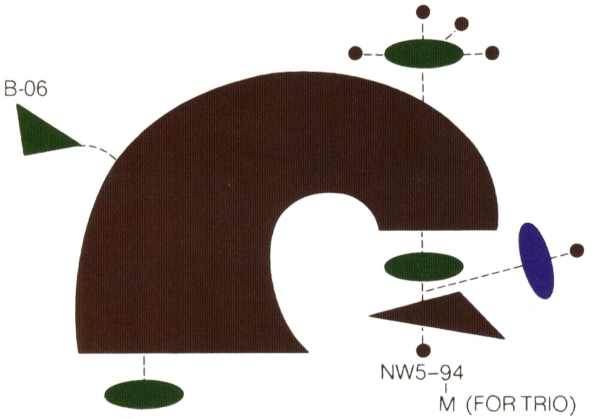
\includegraphics[width=3cm]{images/chapter3/comp76pictitle.png}}}$ (\textit{Composition No. 76})}

        Though Braxton's oeuvre comprises over 400 numbered works (at time of writing), each of them deserving a good deal more scholarly attention than they typically receive, \textit{Composition No. 76} (1977) merits singling out for a few reasons.\footnote{As is customary, I'll be referring to Braxton's works by their catalog numbers rather than by their proper graphic titles. While these titles (and especially their gradual change over the years) are fascinating in their own right, they unfortunately tend to typeset poorly. \textit{Composition No. 76}'s graphic title is given in the section heading.} First, only a relatively small number of his works have been formally published and made available to the general public---and many of these only relatively recently. Of these available works, \textit{No. 76} is by far the most complex in terms of its use of well-defined neo-notations and serves as a local apex in Braxton's musical and intellectual development during his flourishing in the mid-to-late 1970s. In contrast with the majority of individual pieces in Braxton's oeuvre, \textit{No. 76} has attracted some degree of scholarly attention owing, ostensibly, to the excerpted module used as the cover artwork for Braxton's seminal 1978 album \textit{For Trio}.\autocite{Braxton_For_Trio} Prior to widespread availability of Braxton's scores, scholars boldly assessed the work based primarily on speculation surrounding this single module. Finally, in 2018 Paul Steinbeck published ``Improvisation and Collaboration in Anthony Braxton’s \textit{Composition 76}''---likely the most thorough analysis yet of a single Braxton work---in an effort to rectify decades of incomplete scholarship.
    
        Braxton belongs to a rarefied class of musical innovators who consistently orient their artistry toward the future. Using the same working method we ascribe to, say, Miles Davis and Karlheinz Stockhausen, Braxton frequently develops a novel compositional practice seemingly from whole cloth and takes it to a sort of aesthetic conclusion before eventually beginning anew. As such, his works taken as a whole demonstrate an incredible diversity of sound- and process-concepts which are encoded via widely disparate methods. These range from complex, rigorously encoded but unscored solo works, to early post-Webernian works (his term) written entirely in traditional notation, to pieces in the much more recent ``Falling River Music'' scheme written predominantly with strictly connotative, asemantic painting and glyphs. \textit{No. 76} was written during a period in which Braxton consistently worked in several of these composition paradigms at once. As such, it displays a particularly dense, complex notation scheme, indebted to both American and European notational innovators like Cage, Feldman, Stockhausen, et al., as well as to the titans of Afrocentric improvised music on whose transcriptions Braxton cut his teeth.

        Braxton has described \textit{Composition No. 76} in a number of different ways. One of my favorite synopses (taken from Braxton's five-volume \textit{Composition Notes} runs thus:

        \begin{smallquote}
            \textit{Composition No. 76} was conceived as an expanded context for three instrumentalists that attempts to provide terms for creative exploration. The reality of this form was conceived as a dynamic sound continuum that emphasizes the collective interchanges of its composite ensemble - rather than the `wonderful' soloist. [...]

            \vspace{7pt}

            \noindent To experience this work is not to hear a continuous succession of events - in the sense of events that flow from momentum into its next materialization (or `act') - rather in \textit{Composition No. 76} there is a static `dribble of isolated events that come together and apart without any sense of `applied' momentum (or `urgency'). This is a `lifeless' sound space that is somehow happening in spite of itself.\autocite[145--8]{Braxton_1988}
        \end{smallquote}
    
        For a more thorough grasp, one must look to the text of the score itself. Per its copyright page, \textit{Composition No. 76} is a trio for improvising multi-instrumentalists, comprising ``twenty-six pages of three-dimensional notation'' organized into 20 paired modules (labelled \{A1\}--\{A2\} through \{T1\}--\{T2\}\footnote{Mysteriously, a single module, \{E\}, contains three sub-modules; the first of which, \{E1\}, is composed only of a single whole note for Player 2.}) as well as seven pages of unison materials---also apparently modular---to be used in what Braxton dubs ``structural sequences'' throughout the performance.\autocite[149]{Braxton_1988} Though not given expressly in the score, it is clear from the pair of performances on \textit{For Trio} that module pairs may be performed in any order, though all three players take part in each module pair concurrently.
        
        As a brief illustration of performance proceedings, Figure~\ref{fig:a1a2} reproduces the first pair of modules, \{A1\}--\{A2\}---a typical arrangement throughout the piece.
    
                \begin{figure} 
                    \centering
                    \fbox{\includegraphics[width=.9\textwidth]{images/chapter3/a1a2.png}}
                    \captionsetup{width=.5\textwidth}
                    \caption[Module pair \{A1\}--\{A2\} from \textit{Composition No. 76}.]{Module pair \{A1\}--\{A2\} from \textit{Composition No. 76}.\footnotemark}
                    \label{fig:a1a2}
                \end{figure}
                    \footnotetext{\autocite[]{Braxton_1977}.}
    
        Over the course of each pair of modules, each player reads from left to right, either engaging in a more-or-less traditional fashion with the materials on standard staves (all three players in \{A1\}) or engaging with these seemingly opaque constellations of staff-fragments and geometric shapes as launchpads for constrained improvisation (players \#1 and \#2 in \{A2\}). The following section will be dedicated to a full unpacking of these materials so as to facilitate further discussion.
        % Though it may at first glance seem rather opaque, Braxton's detailed instructions allow \textit{No. 76} to be broken down into more graspable constituent glyphs. As an example, using the above figure as a reference and moving left to right on the page, we find:
    
        % \begin{smallquote}
        % \begin{enumerate}
        %     \item A bespoke glyph preceding \textbf{A1} indicating that all players are to match the instrument chosen by performer \#1
        %     \item A bespoke glyph indicating that all players are to match tempi
        %     \item The diamond clef ($\diamond$), Braxton's long-standing symbol which indicates that the following material may be read in any transposition
        %     \item Traditional dot-stem-beam notation in purple ink featuring fixed dynamics and the star accidental ($\star$) which stands in for either a sharp or a flat per the player's discretion.
        %     \item Traditional notation in black followed by Braxton's bespoke ``rest'' symbol, the diagonal double-headed arrow.
        %     \item A cue point at \textbf{A2}, whereupon two players enter into dense ``open material'' (to be discussed in greater detail anon.)
        % \end{enumerate}
        % \end{smallquote}
        
    \subsubsection{Braxton's fixed material}

        In Volume D of his 1988 \textit{Composition Notes}, Braxton describes \textit{No. 76} as fundamentally composed of ``fixed'' and ``open materials.'' As Steinbeck notes, though, these terms (at least under their typical usage) are essentially unable to fully capture the subtlety with which Braxton approaches his encoding scheme.\autocite[254]{Steinbeck_2018} Braxton seems to take this fundamental division between the ``fixed'' and the ``open'' quite seriously---to the point that his performance instructions are delivered across two pages: one dedicated to each primary category of notation. Table~\ref{tab:braxtoninstructions1} below reproduces in full Braxton's neo-notational glyphs used in this fixed material---featuring both his stated instructions as well as my categorization of each glyph according to the modified Ligetian typology established in the last chapter. The granularity with which Braxton's notation operates necessitates two new terms in describing these symbols: 
        
            \begin{smallquote}
                \begin{enumerate}
                    \item \textit{inducement}---a glyph which by itself invokes a certain FOP in a performer, leading to the execution of some gesture and a resultant sound. (We might take the traditional example: an individual note-head, which signifies that some action is to be taken to produce sound.)
                    \item \textit{modifier}---to contrast, a glyph which is used to modify some FOP by being appended to an inducement in one way or another. By itself (under normal circumstances) a modifier would not result in the performer taking any particular action---it is only when appended to a sounding glyph that a modifier can affect sonic results. (For example: the flags, beams, dynamic markings, and articulations which accompany the note-head).
                \end{enumerate}
            \end{smallquote}
       
        As seen in the previous chapter with Braxton's early ``Ghost Trance'' notation, it is possible to deploy a highly stripped-down notation scheme---that is, one which eschews most modifiers in favor of only barely-adorned inducements. In this case, Braxton seeks to deliberately leave the bulk of the parameters normally described by a more full-featured notation up to the performer and thus omits those glyphs which would typically delineate said parameters. Nevertheless, ``Ghost Trance Music'' as well as every other notation scheme examined here (result, action, recipe, et al.) can be meaningfully described as some arrangement of various inducements and modifiers. Using these definitions, Table~\ref{tab:braxtoninstructions1} presents and describes each novel symbol given on \textit{Composition No. 76}'s first page of instructions. 
        
        %As demonstrated in the previous chapter, semantically coherent systems of notation can be deployed which use barely-adorned inducements---necessarily very loosely constrained insofar as they do not feature the typical modifiers which would accompany them in traditional notation. However, under every coherent notation scheme we've encountered thus far, any of the notational sub-types (result, action, recipe) may comprise many different inducements and modifiers---and as we will see given Braxton's detailed instruction set, this scheme is no exception.

   % Despite the wide latitude granted to performers, per Braxton's understanding everything preceding \textbf{A2} is considered ``fixed material.'' Insofar as the symbols involved in are concerned, I have taken the liberty of reproducing the table provided with the instructions below in full for ease of reference in~\ref{tab:braxtoninstructions1}.
    
    
        \begin{table}
        \NewTableCommand\myhline{\hline[0.1em]}
            \scriptsize
            \centering
            \singlespacing
                \begin{tblr}{
                cells={valign=m, halign=l},
                width=\textwidth,
                colspec={l X[2.5] X[1] X[-5]},
                column{3}={halign=c}
                }
                    \myhline
                    & \textbf{Instruction given} & \textbf{Symbol} & \textbf{Comment}\\ [0.5ex]
                    \myhline
                    \textbf{1.} & ``Match dynamics'' 
                        & $\vcenter{\includegraphics[width=1cm]{images/chapter3/instructions/01.png}}$ 
                        & Relational, interpersonal. Recipe, modifier. Constrains dynamics. \\
                    \textbf{2.} & ``Match dynamics but very softly'' 
                        & $\vcenter{\includegraphics[width=1cm]{images/chapter3/instructions/02.png}}$ 
                        & (as above) \\
                    \textbf{3.} & ``Play note then improvise for small amount of time'' 
                        & $\vcenter{\includegraphics[width=1cm]{images/chapter3/instructions/03.png}}$ 
                        & Recipe, inducement. No appreciable constraint. \textit{Appears in instructions but not in score.}\\
                    \textbf{4.} & ``Hold until next cue point (suspension)'' 
                        & $\vcenter{\includegraphics[width=1cm]{images/chapter3/instructions/04.png}}$ 
                        & Relational, interpersonal. Recipe, modifier. Fixed based on prior action taken. \\ 
                    \textbf{5.} & ``Prepare just before time cue (and then execute)'' 
                        & $\vcenter{\includegraphics[width=1.5cm]{images/chapter3/instructions/05.png}}$ 
                        &  Modifier. Restricts onset time for execution of phrase.\\
                    \textbf{6.} & ``Cue for someone else [...]'' 
                        & $\vcenter{\includegraphics[width=1cm]{images/chapter3/instructions/06.png}}$ 
                        & Strictly informational. Orients performer with regard to other events in the score. \\
                    \textbf{7.} & ``Can be used for vocal phrase'' 
                        & $\vcenter{\includegraphics[width=1cm]{images/chapter3/instructions/07.png}}$ 
                        & Modifies improvisatory inducements. Relaxes constraint by expressly permitting vocal execution.\\
                    \textbf{8.} & ``Wait for near the end of the time group to finish phrase point [...]''
                        & $\vcenter{\includegraphics[width=1.5cm]{images/chapter3/instructions/08.png}}$
                        & Relational, contingent on elapsed time. Recipe, modifier.\\
                    \textbf{9.} & ``Rest'' 
                        & $\vcenter{\includegraphics[width=1.5cm]{images/chapter3/instructions/09.png}}$
                        & Result notation (silence), inducement. Duration potentially contingent on other players' actions.\\
                    \textbf{10.} & ``Match instrument (that principle figure in time zone is playing) [...]''
                        & $\vcenter{\includegraphics[width=1cm]{images/chapter3/instructions/10.png}}$
                        & Relational, interpersonal. Recipe, instrumental constraint. Modifier.\\
                    \textbf{11.} & ``Change dynamics abruptly for next playing section [...]'' 
                        & $\vcenter{\includegraphics[width=.7cm]{images/chapter3/instructions/11.png}}$
                        & Relational, self. Recipe, dynamic constraint. Modifier. FOP excludes prior dynamic attributes.\\
                    \textbf{12.} & ``Rest for 3 to 5 seconds'' 
                        & $\vcenter{\includegraphics[width=1.5cm]{images/chapter3/instructions/12.png}}$
                        & Result notation (silence), inducement. \\
                    \textbf{13.} & ``Change instrument quickly'' 
                        & $\vcenter{\includegraphics[width=1.5cm]{images/chapter3/instructions/13.png}}$
                        & Relational, self. Recipe, instrumental constraint, modifier.\\
                    \textbf{14.} & ``Independent tempo'' 
                        & $\vcenter{\includegraphics[width=1.5cm]{images/chapter3/instructions/14.png}}$
                        & Relational, interpersonal. Recipe, tempo constraint, modifier. Unclear if tempo \textit{must} be distinct or merely ``uncoupled''.\\
                    \textbf{15.} & ``Match tempo [...]'' 
                        & $\vcenter{\includegraphics[width=1.5cm]{images/chapter3/instructions/15.png}}$
                        & Relational, interpersonal. Recipe, tempo constraint, modifier.\\
                    \textbf{16.} & ``Open clef'' 
                        & $\vcenter{\includegraphics[width=.7cm]{images/chapter3/instructions/16.png}}$
                        & Modifier. Relaxes constraint on phrase execution by incorporating transposition into FOP.\\
                    \textbf{17.} & ``Sharp or flat'' 
                        & $\vcenter{\includegraphics[width=.7cm]{images/chapter3/instructions/17.png}}$
                        & Modifier. Relaxes constraint on note execution by incorporating transposition into FOP.\\
                    \myhline
                \end{tblr}
        \captionsetup{width=.5\textwidth}
        \caption[Composer-provided list of symbols from Braxton's \textit{Composition No. 76}]{Composer-provided list of symbols from Braxton's \textit{Composition No. 76}.\footnotemark}
        \label{tab:braxtoninstructions1}
    \end{table}
        \footnotetext{\autocite[instructions pg. 1]{Braxton_1977}.---Index numbers in this case correspond with those provided in the score.}

       Fixed notation in \textit{No. 76} might be thought of as a heavily-modified form of traditional notation insofar as it features (1) traditional ${time}\times{pitch}$ mapping on the $x$- and $y$-axes; (2) (some) traditional clef indications; (3) phrases expressed using the dots, stems, and beams of traditional notation; and (4) other traditional modifiers such as dynamic markings, articulations, and fermate. 
    
       This is by and large the extent to which Braxton imports familiar symbols. However, certain neo-notational glyphs replicate or tweak traditional functions despite their novel form. The new clef (16.) and new accidental (17.) (both long-time Braxton staples) in essence serve the same purpose as their familiar counterparts, merely adding another degree of openness to the score's realization by reducing constraints typical to a given musical passage. The bespoke symbol for ``rest'' (without modifier at 9. and with duration indication at 12.) simply serves as a proportional stand-in for typical absolute-duration rests. Likewise, while Braxton's new cuing symbols (5. and 6.) fill an important role in that they aid players in orienting themselves within material, they ultimately replicate functions available in traditional notation as well. (Color, insofar as it is featured in fixed material, also serves a ``tweaked'' traditional role, though I'll expand on this in a coming section.)
       
       We also find, however, that Braxton employs many symbols which fulfill roles not typically found in traditional notation. Specifically, his novel relational symbols serve as important additions for a music which seeks to systematically constrain improvisers' creative output. That is to say: instructions 1., 2., 4., 8., 10., 11., 13., 14., and 15. all serve to mediate a performer's actions not based on a desired sonic product per se (i.e. some absolute factor) but instead based on the \textit{relation} between the player and some other variable---either another player's actions (as in the ``match dynamics'' or ``match tempo'' indications) or one's own prior decisions (``change instrument quickly'' or ``change dynamics abruptly''). In both of these cases, the final outcome results from a confluence of an individual player's choices, all players' actions as a group, and the composer's meta-constraints established pre-performance.
    
       Of course, relational parameters are not exclusive to neo-notation. Dynamic markings and expressive texts found in traditional notation tacitly rely on relational parameters. For example, when I read \textit{ritardando} the precise rate of my slowdown depends upon that of my stand-mate. Likewise, the increase in amplitude from \textbf{\textit{p}} to \textbf{\textit{f}} is contingent on the loudness of my initial expression. However, symbols like Braxton's \#8., 14. or 15. which \textit{deliberately} (rather than incidentally) parametrize the gestures and sonic products of other performers are essentially foreign to the encoding schemes familiar to most musicians. Here, Braxton is making explicit what were predominantly implicit characteristics of prior notations.
    
    \subsubsection{Braxton's open material}

            \begin{figure} 
                \centering
                \fbox{\includegraphics[width=.4\textwidth]{images/chapter3/openf1.png}}
                \captionsetup{width=.55\textwidth}
                \caption[Open sub-module \{F1\} from \textit{No. 76}.]{Open sub-module \{F1\} from \textit{No. 76}.\footnotemark}
                \label{fig:openf1}
            \end{figure}
                \footnotetext{\autocite[]{Braxton_1977}.}
            
        \textit{No. 76}'s open material is easily distinguishable by spatial separation (``floating'' on the page without being tethered to a single staff) and by its geometry. Here we find the three-dimensionality Braxton referenced earlier: staves in open material are fragmentary and clef-less; seeming to emerge from and recede into the page as though they were two-dimensional projections of massy objects in space. Though now accompanied by constellations of modifier symbols, play is still oriented around these staff fragments, which may be approached non-linearly: that is, in any order. Per Graham Lock, it appears that an adequate realization of these sub-modules requires that each staff-fragment be interpreted, though in no particular order.\autocite[Postscript 3]{Lock_1989}
    
        In practice, a single ``unit'' of open notation consists of a staff-fragment in some orientation (implying a particular positionality in three-dimensional space). Notes inscribed on these staff-fragments typically appear in color, though they may also be rendered in the traditional black. Almost universally, these staff fragments are modified by an attached simple geometric shape filled with color. These appear to the reader to be ovals (full or truncated), irregular triangles, and skewed quadrilaterals, but are almost certainly intended to be equilateral triangles, squares, and circles subjected to the same system of projection as the staff fragments. Modifying these colored shapes are short sequences of numeric code. Finally, each open sub-module features one or more ``linking'' gestures comprising staffless eighth-note figures in black which share stems with two staff fragments (as shown above in Figure~\ref{fig:openf1}). 

        All explicit instructions pertaining to open material are given on the second instruction page and are reproduced in Table~\ref{tab:braxtoninstructions2} below. 

        \begin{table}
        \scriptsize
        \centering
        \singlespacing
            \begin{tblr}{width=.8\textwidth, colspec={l X[2.5] X[-2.5]}}
                \hline[0.1em]
                 & \textbf{Information} & \textbf{Note} \\ 
                \hline[0.1em]
                \textbf{A.} & $\vcenter{\includegraphics[width=4cm]{images/chapter3/instructions/instA.png}}$
                    & $\vcenter{Numbers indicate number of notes/phrases per improvisatory sub-module (?). They may be modified with parentheses or squares.}$\\
                \textbf{B.} & $\vcenter{\includegraphics[width=3cm]{images/chapter3/instructions/instB.png}}$
                    & $\vcenter{Improvisatory indices may also be modified with $\times$ or $(\times)$ indicating mandatory or optional use of vocals for improvisation.}$\\
                \textbf{C.} & $\vcenter{\includegraphics[width=5cm]{images/chapter3/instructions/instC.png}}$
                    & $\vcenter{Relational signifiers orienting improvisation in one of three ways with regard to other performers.}$\\
                \textbf{D.} & $\vcenter{\includegraphics[width=5cm]{images/chapter3/instructions/instD.png}}$
                    & $\vcenter{Expressly indicates presence of performer-mapping as critical component of performance.}$\\
                \hline[0.1em]
            \end{tblr}
            \captionsetup{width=.5\textwidth}
        \caption[Supplementary instructions from Braxton's \textit{Composition No. 76}.]{Supplementary instructions from Braxton's \textit{Composition No. 76}.\footnotemark}
        \label{tab:braxtoninstructions2}
            \end{table}
                \footnotetext{\autocite[instructions pg. 2]{Braxton_1977}.---Note that Braxton opts not to concretely define the fundamental unit of improvisatory action signified by the numeric code. Steinbeck claims it might refer either to notes or phrases.}

        As is clear from the given instructions, Braxton's open material is still subject to rather stringent restrictions. In its execution, open material is divided into clusters of improvised gestures induced by each staff-fragment/shape combination. These clusters comprise a rendering of the modified-traditional notation within the staff-fragment as well as a series of notes or phrases delimited by the codes of the form \{$+\:i + j +... + n$\}. Parenthetical or square modifiers indicate a change of instrument in between soundings or the use of the AACM signature ``little instruments'', respectively.\footnote{\autocite[170]{Jost_1994}.---A ``little instrument'' is a (typically small) auxiliary percussion or wind instrument deployed to add color or break up the prevailing texture. These include but are not limited to ``slide whistles, recorders, harp, Japanese koto, harmonica, kazoo, police whistles, thunder sheet, bells and gongs, plus countless other percussion instruments.''} Elements of the numeric code may be accompanied by $\times$ or $(\times)$, indicating mandatory or optional use of the voice in the specified improvisation-group.
    
        Open material features its own bespoke relational signifiers. \textsc{dom}, \textsc{supp}, and \textsc{op} indicate that an improvisatory cluster should either dominate, support, or remain un-coupled from the prevailing ensemble texture. These are distinct from the ``fixed'' relational symbols in that they demand significantly more creative interpretation---i.e. restrict a performer's FOP much less. Where ``match dynamics'' or ``change instrument quickly'' are rather straightforward in their interpretation and feature very little ambiguity, \textsc{dom} and \textsc{sup} modifiers are not merely functions of greater/lesser dynamic or density. Rather, they require a performer to assess in-the-moment the sort of gesture which befits a given sonic environment from among an essentially infinite array of potential actions.

    % \begin{notestuff}
    %     This verges on too much commentary for this dry, explanatory section---I'm gonna return to it later.
    % \end{notestuff}

        Braxton's distinct use of color in \textit{No. 76} almost certainly accounts for a significant portion of interest (scholarly or otherwise) in the score. Per Table~\ref{tab:braxtoninstructions2}, the only instruction explicitly given in the text with regard to color is the rather vague pronouncement that ``color of shape is emotional subjective interpretation.'' Of course, colored inks not only appear in the geometric figures, but were used to inscribe both open and fixed phrases as well. Graham Lock, perhaps the most widely-read Braxton scholar, describes the intentions behind this color scheme in a footnote:
        
            \begin{smallquote}
                The colour code to \textit{Composition 76} is actually based on astrological correspondences. That is, Braxton selected a set of the emotional characteristics attributed to various signs of the zodiac and then designated them in the score by using the colours associated with the same signs. The code is: blue = sombre or moody (Saggitarius); red = explosive or intense (Aries); green = calm, restrained or contained (Taurus); violet = vibrant or pulsing or energetic or vigorous (Pisces); brown = complementary or harmonious or balancing (Libra); yellow = strong, lyrical or bright (Leo).\autocite[222]{Lock_1989}
            \end{smallquote}
        
        In a related 2008 paper, Lock reiterates much of the same information but adds:
        
            \begin{smallquote}
                Shades of colour mark factors such as dynamic and tempo: the darker the hue, the faster and/or louder you play.\autocite{Lock_2008}
            \end{smallquote}
    
        That Braxton opts not to disclose this important scheme in the text of his score is interesting in and of itself and will be revisited in a later section. For now, though, it suffices to say that taken whole, the graphic elements in his open material are neither fully denotative nor fully connotative. If we take the code given by Lock at face value, color inside shapes (and presumably when applied to traditional notation as well) serves essentially as once-abstracted expressive text which applies to a given improvisatory expression; a stripped-down rendering of instructions of the form ``\textit{con eleganza},'' ``\textit{molto agitato},'' ``\textit{doloroso},'' etc. Clearly, however, certain aspects of these signs remain un-coded. The shapes' forms, for instance; their precise positioning relative to the staff fragments; the virtual orientation of the staff fragments themselves with respect to the viewer---each of these factors poses a ``graphical excess'' connoting additional factors which appear to be strictly performer-mapped.\footnote{\autocite{Dicker_2016}.---These symbols recur frequently throughout Braxton's oeuvre and are discussed at length (independent of any one composition) in his \textit{Tri-Axium Writings} and elsewhere. They make their most prominent appearance in his later ``Ghost Trance Music'' composition series, where they serve as ``jumping-out'' points where performers leave the prevailing (written) musical material to improvise before returning at another iteration of the same symbol. Triangle, square, and circle correspond to, respectively: ``synthesis or correspondence logics;'' ``stable logics;'' ``mutable logics.''}
    
        Worth noting is that at a base level, Braxton's open notation functions much in the same way as his fixed material: i.e. by providing sequences of inducements flanked by various modifiers. This is very much not a given for other forms of un-coded open notation, which may well bundle together graphic elements in such a way that individual glyphs are impossible to parse as providing any one particular function (e.g. Cardew's inscriptions in \textit{Treatise} discussed last chapter).

        % \begin{notestuff}
        %     This raises a very important point about the notion of ``completeness'' of representation of sound- or process-concepts in the written score. It seems like the 19th-century ``Eurological'' model would always have it that the composer's S/PCs should be represented as entirely as possible in the written score, while for Braxton this is obviously not the case. This merits a good bit of discussion in the comparative section!
        % \end{notestuff}

    % \begin{uselater}
    % \begin{smallquote}
    %     The musician can enter the module at any point, and go around it in any direction. ... All primary shapes (circle, triangle, oblong etc.) are in colour (as is some of the notation) and designate improvisation, the different colours and shapes indicating the kinds of improvisation to be played ... \autocite[Postscript 3]{Lock_1989}
    % \end{smallquote}
    % \end{uselater}

    \subsubsection{Unknowns}

        Despite its position as one of Braxton's most-discussed works (and despite Braxton's own commentary in his \textit{Composition Notes}), certain notational elements still remain fundamentally opaque; either by design or because of incomplete knowledge on the part of its analysts. For completeness' sake, I'll reproduce these here in Table~\ref{tab:mysteryglyphs}.

            \begin{table}
                \footnotesize
                \centering
                \singlespacing
                    \begin{tblr}{width=.7\textwidth, colspec={l X[2.5] X[-3.5]}}
                        \hline[0.1em]
                         & \textbf{Information} & \textbf{Note} \\ 
                        \hline[0.1em]
                        \textbf{1.} & $\vcenter{\includegraphics[width=2.5cm]{images/chapter3/mystery01.png}}$
                            & $\vcenter{``Mirrored-C'' or ``$\mathscr{X}$'' clef which occurs sporadically throughout the score.}$\\
                        \textbf{2.} & $\vcenter{\includegraphics[width=2.5cm]{images/chapter3/mystery02.png}}$
                            & $\vcenter{Action notation in the form of sinusoidal line in structural sequences.}$\\
                        \textbf{3.} & $\vcenter{\includegraphics[width=1cm]{images/chapter3/mystery03.png}}$
                            & $\vcenter{Rectangular notehead in structural sequences.}$\\
                        \textbf{4.} & $\vcenter{\includegraphics[width=4cm]{images/chapter3/mystery04.png}}$
                            & $\vcenter{Example of additional numeric code appended to each open sub-module. Not to be confused with improvisation modifiers shown in Table~\ref{tab:braxtoninstructions2}.}$\\
                        \hline[0.1em]
                    \end{tblr}
                    \captionsetup{width=.5\textwidth}
                \caption[Glyphs of unknown significance in \textit{Composition No. 76}.]{Glyphs of unknown significance in \textit{Composition No. 76}.\footnotemark}
                \label{tab:mysteryglyphs}
            \end{table}
            \footnotetext{\autocite{Braxton_1977}.}

        Listening to the two ``canonical'' extant recordings yields some insight. First: A simple whole-note figure using the un-referenced ``mirrored-C'' or ``$\mathscr{X}$'' clef results in distinct chords in the two versions (shown below in Figure~\ref{fig:mysteryclef}). A fair assumption might be that the clef serves as a yet more open version of the diamond clef where onset and duration are relatively fixed and precise pitch is held open. This seems to be confirmed by Tri-Centric Foundation Archives manager Carl Testa, who, in reference to a sketch of the much-earlier \textit{Composition No. 6E} (1968), writes that ``[t]he score features an ``X'' clef which indicates to the performers that exact pitch reproduction is not required [...]'' (though the glyphs do not match precisely).\autocite{Testa}

            \begin{figure}
                \centering
                \subfloat[\centering in score]
                {{\fbox{\includegraphics[width=.18\textwidth]{images/chapter3/moduleP2mysteryclef2.png} }}}%
                \qquad
                \subfloat[\centering transcription (conc.)]{{\fbox{\includegraphics[width=.3\textwidth]{images/chapter3/moduleP2mysteryclef.png} }}}%
                \captionsetup{width=.55\textwidth}
                \caption[``Mirrored C'' or ``$\mathscr{X}$'' clef at sub-module P2 in V1/V2 on \textit{For Trio}.]{``Mirrored C'' or ``$\mathscr{X}$'' clef at sub-module P2 in V1/V2 on \textit{For Trio}.\footnotemark}%
                \label{fig:mysteryclef}%
            \end{figure}
            \footnotetext{\autocite[2:27--3:18 of Version 1 and 4:44--6:03 of Version 2]{Braxton_For_Trio}.}

        Next: The sinusoidal line typically reserved to signify trills in other works seems to indicate open improvisation with a duration limited by cues. Performances on the album render this symbol using rapid switches between instruments, long tones, short bursts of sound, etc., and vary considerably in length. The rectangular notehead (resembling the \textit{maxima} from medieval/Renaissance mensural notation) occurs infrequently, but seems to be rendered simply as a slightly longer quarter-note pulse. Lastly and perhaps most mysteriously: I can find no reference to the ``secondary'' numeric codes which appear appended to each open sub-module. Unlike their coded counterparts which describe attributes of improvisatory ``clusters,'' numbers in these secondary codes appear signed (either ``$+$'' or ``$-$'') and include fractional values---neither of which pertain to the prior code given above in Table~\ref{tab:braxtoninstructions2}. Again, as is often the case in Braxton's work, it remains unclear whether these symbols' lack of well-defined function (at least as explained in the score) serves as a deliberate omission or an oversight, or whether perhaps their function was so clear to the participants as to have made their explicit definition unnecessary. I will return in greater detail to this notion in a later section.

            \begin{center}
            \vspace{-10pt}
            \noindent\rule{3cm}{0.4pt}
            \end{center}

        % WRAP-UP PARAGRAPH
        Thus, an individual performance of \textit{Composition No. 76} proceeds as follows: Pre-performance, performers decide upon a particular ordering of module-pairs and fixed structural sequences. In executing these module-pairs, players seamlessly slip between engagement with more restricted linear interpretation of fixed materials and omnidirectional interpretation of open materials; all the while maintaining certain temporal, dynamic, and structural relations with regard to other performers. Though Braxton thinks of these fixed and open performance paradigms as distinct modes of play, it's clear from examining the notation that this distinction is, in the end, quite blurry.
    
        Before moving on to discuss the import of Braxton's notational choices, however, I would like to pivot rather abruptly to another work-complex by an unlikely kindred spirit---one in whose work we'll see many noteworthy parallels and perpendiculars.
    
\subsection{\textit{Das Andere} \& Op. 89 \textit{``before the universe was born''}}

        In contrast with other composers willingly or unwillingly linked to the spectralist paradigm, Horațiu Rădulescu has, for a variety of reasons, received considerably less scholarly attention. Known among fans and detractors alike for his outsize personality, his ``convoluted, jargon-heavy writing'', and most of all for his highly idiosyncratic sound worlds, Rădulescu parallels Braxton insofar as he is often seen as an ``outsider'' in his field.\autocite{Suckling_2018} More than anything else, Rădulescu's particular flavor of spectralism is characterized by a fascinating form of sonic indeterminacy he dubs \textit{sound plasma}. So dense and poly-timbral as to resist traditional descriptors, \textit{sound plasma} comprises a range of techniques including ``sparkling, irregular trill[s],'' ``irregular arpeggios [...] with extreme \textit{flautando} bowing,'' and ``irregular, breathy `phase shifting' timbre[s],'' all of which combine in myriad ways to (ideally) produce the galaxies of resultant sum and difference tones which Rădulescu seeks.\autocite{Heery_2016}
                
        This section concerns a work-complex comprising two of Rădulescu's compositions, \textit{Das Andere} (1984) and Op. 89, \textit{``before the universe was born''} (1995), for unaccompanied viola and string quartet, respectively---two pieces which epitomize his pursuit of this elusive \textit{klangwelt}. For R\u{a}dulescu, \textit{Das Andere} represented an early attempt to solve the problem of adapting plasmatic music---usually reliant on complex, chaotic interactions between multiple sounding bodies---to a single instrument\autocite[10]{Marinescu}  To that end, he developed a fascinating, singular notation scheme to facilitate his measured indeterminacy. Evidently, this experimental foray was successful enough that he continued to deploy elements of \textit{Das Andere}'s notation throughout his career (albeit with various mutations), including in Op. 89.\footnote{This fact is noteworthy in and of itself given that experimental notations typically fail to live past the age of a single piece.} 

        Of R\u{a}dulescu's predilection for new notations, Liviu Marinescu explains:

            \begin{smallquote}
                [...] his desire to notate differently came from the need to compose differently. [...] For centuries, the Western world had worked slowly on developing a notation system that removed approximation between what was seen, what was played, and what was ultimately heard. Horațiu Rădulescu saw this old routine as a significant obstacle in the creation of plasmatic music, which is why he sought to return much of the initiative and creative power back to the performer.\autocite[1]{Marinescu}
            \end{smallquote}

        \noindent In the following sections, I will demonstrate precisely how and to what extent R\u{a}dulescu was able to achieve this ``transfer'' by closely examining the unique notational syntax and semantic content developed for these two pieces.

    \subsubsection{Rădulescu's notation scheme---denotative factors}
        
        Notation in \textit{Das Andere}/Op. 89 is a form of \textit{tablature}---a subset of action notation which encodes actions pertaining to the relationship between player and instrument-body.\footnote{This is to say: per Chapter 2, syntactic relations between signs in tablatures do not map to resultant sounds in the same way they would in result notations like our traditional pitch-centric notation.}. \textit{Das Andere} (being the simpler case) features staff lines representing the four strings of the viola, arranged from high to low.\footnote{
            To be precise, Instruction pg. 1 subtitles the piece ``for a stringed instrument tuned in perfect fifths.'' R\u{a}dulescu has since published an alternate score for 'cello which he also suggests be used for violin or double bass.
            } 
        As in traditional guitar/lute tablatures, most symbols used in Rădulescu's system reflect positions for the player's left hand. Unlike guitar tablature, however, where fret positions represent the subdivision of a particular string into sectors allowing for pitches in 12-tone equal temperament, numeric position values in Rădulescu's works most often represent the locations of natural harmonics on the string. For instance, a ``7'' on the uppermost staff line would indicate that the player ought to place a finger at the 7th-harmonic position on string I of the viola. Also unlike traditional tablature, this position marker by itself does not signify a particular sounding---as when one plucks a harmonic on guitar incited by ``$\diamond$'', for example. Rather, \textit{Das Andere} and Op. 89 feature specific sets of actions meant to sound these harmonics in different ways. 
    
        There are two primary sets of actions Rădulescu employs in the pieces (which he analogizes as ``play characters'' in his supplementary material represented by \textit{alpha} ($\newalpha$) and \textit{sigma} ($\Upsigma$) in the score.\autocite[dedication page]{Radulescu_1984} Given that these function as mutable, flexible notations which themselves might be modified by subsidiary symbols, I think of these as ``second-order'' notations which cluster together complex performance parameters into comparatively neat packages; much in the way that the baroque ``turn'' reduces a complex set of actions down to a single glyph, which itself is modified by key signature, tempo, meter, etc.
    
        In a series of instruction pages provided with \textit{Das Andere}, Rădulescu gives quite detailed instructions regarding the execution of each of these primary and subsidiary second-order symbols. For instance, regarding the first such symbol in \textit{Das Andere}, $\Upsigma$, he gives:
    
            \begin{smallquote}
                The $\Upsigma$ modules of biphony are to be performed as very irregular melodies resembling high Alp-horns. When dynamically very loud, the ``colliding'' pitches of the double stops produce differential sounds ($\delta$). Their very irregular melodic shape should never use periodic rhythm or glissandi.
                
                \vspace{7pt}
                
                \noindent Play always \textit{legatissimo} (and as much as possible \textit{liscio}, i.e. changing the bow direction unobtrusively). The dynamic should vary within a wide range in order to shape the macro-form. Simultaneously the dynamic of the micro-forms works independently and sometimes even contradictory to the global one. The micro climaxes of the [v-figure] should not be played as sforzandi but instead as high speed crescendi/decrescendi. [...] 
                
                \vspace{7pt}
                
                \noindent Even with increased bow-pressure noise in the very high register, the natural harmonics used by $\Upsigma$ should always sound beautifully rough, primitive and wild like imaginary high Alp-horns. Do not filter them whistle-like pitches.\autocite[Instruction pg. 1]{Radulescu_1984}
            \end{smallquote}

        \noindent Likewise, for $\newalpha$, he gives:

            \begin{smallquote}
                The $\newalpha$ [...] technique consists of very irregular arpeggios [graphic] with very F (flautando) and $\nwsearrownew$ (fast bowing), and with a lot of point of contact changes $\pm \text{VP} \leftrightarrow \text{MT}$.

                \vspace{7pt}
        
                \noindent The chord components must be allowed to resonate (lasciar vibrare), and when the score contains blank segments between the flourishes of apreggios, the [\textit{u du 'u du}] or [\textit{little devils}] technique (the ``obsessive voice'' $\usym{27A1}$) is to be performed.

                \vspace{7pt}
        
                \noindent Thus all the $\newalpha$ sequences are fast and aperiodic dialogues between the arpeggios and the momentary $\usym{27A1}$, releasing rich timbre, pitch and register information like an irregularly perforated polyphony.\autocite[Instruction pg. 3]{Radulescu_1984}
            \end{smallquote}

        Rădulescu's neonotation, including these ``play characters,'' the lesser second-order symbols, and associated modifiers are reproduced below in Table~\ref{tab:radinstructions1} and Table~\ref{tab:radadditional}.
    
            \begin{table}
                \scriptsize
                \centering
                \singlespacing
                    \begin{tblr}{
                    width=.9\textwidth,
                    cells={valign=m, halign=l},
                    colspec={l X[2] X[1] X[-2] },
                    column{3}={halign=c}
                    }
                        \hline[0.1em]
                        & \textbf{Definition} & \textbf{Symbol} & \textbf{Comment}\\ [0.5ex]
                        \hline[0.1em]
                        \textbf{1.} & ``Open string''
                            & $\vcenter{\includegraphics[width=1cm]{images/chapter3/radinstructions/01openstring.png}}$
                            & Basic indication that note to be played is not a harmonic but on open string. Recipe notation, inducement. \\
                        \textbf{2.} & ``Multiphonic''
                            & $\vcenter{\includegraphics[width=1cm]{images/chapter3/radinstructions/02multiphonic.png}}$
                            &  Multiphonic on one string. May be modified by other glyphs. Recipe, inducement.\\
                        \textbf{3.} & ``U du `u du''---``phase shifting bow; rebouncing of the bow in between two imaginary walls; with rigid arm''
                            & $\vcenter{\includegraphics[width=1cm]{images/chapter3/radinstructions/03udu.png}}$
                            & Shorthand for specific body-action constraints in service of a particular indeterminate but constrained sound-field. Recipe, inducement.\\
                        \textbf{4.} & ``Little devil''---``high melody of natural harmonics (via unstable [harmonic] played with only one finger [...])''
                            & $\vcenter{\includegraphics[width=1cm]{images/chapter3/radinstructions/04devil.png}}$
                            & (As above.)\\
                        \textbf{5.} & ``Sigma ($\Upsigma$)''---``[...] two very high but powerful simultaneous melodies of natural harmonics [...]''
                            & $\vcenter{\includegraphics[width=1cm]{images/chapter3/radinstructions/05sigma.png}}$
                            & ``Second-order'' symbol modified by harmonic indications which induces complex ``micro-improvisatory'' gestures. Recipe, inducement.\\
                        \textbf{6.} & ``Alpha ($\newalpha$)''---``arpeggios of open strings [...] using very aperiodical micro rhythm''
                            & $\vcenter{\includegraphics[width=1cm]{images/chapter3/radinstructions/06alpha.png}}$
                            & (As above.)\\
                        \textbf{7.} & ``High natural harmonics''---``high natural harmonics in LASCIAR VIBRARE [...] alternating with the open string''
                            & $\vcenter{\includegraphics[width=1cm]{images/chapter3/radinstructions/07highharm.png}}$
                            & (As above.) \\
                        \textbf{8.} & Bow speed---slow
                            & $\vcenter{\includegraphics[width=1cm]{images/chapter3/radinstructions/08bowslow.png}}$
                            & Modifier. \\
                        \textbf{9.} & Bow speed---fast
                            & $\vcenter{\includegraphics[width=1cm]{images/chapter3/radinstructions/09bowfast.png}}$
                            & (As above.) \\
                        \textbf{10.} & Bow pressure---flautando
                            & $\vcenter{\includegraphics[width=1cm]{images/chapter3/radinstructions/10flaut.png}}$
                            & (As above.) \\
                        \textbf{11.} & Bow pressure---premuto
                            & $\vcenter{\includegraphics[width=1cm]{images/chapter3/radinstructions/11prem.png}}$
                            & (As above.) \\
                        \textbf{12.} & Phonetic rhythm---synchronous
                            & $\vcenter{\includegraphics[width=1cm]{images/chapter3/radinstructions/12phonetic_sync.png}}$
                            & Modifier pertaining to phonetic rhythm of \textit{Tao Te Ching} inscriptions. \\
                        \textbf{13.} & Phonetic rhythm---shifted
                            & $\vcenter{\includegraphics[width=1cm]{images/chapter3/radinstructions/13phonetic_shifted.png}}$
                            & (As above.) \\
                        \hline[0.1em]
                        \end{tblr}
                \captionsetup{width=.5\textwidth}
                \caption[Composer-provided list of symbols from Rădulescu's String Quartet No. 5 (1993), used also in \textit{Das Andere} (1984)]{Composer-provided list of symbols from Rădulescu's String Quartet No. 5 (1993), used also in \textit{Das Andere} (1984).\footnotemark}
                \label{tab:radinstructions1}
            \end{table}
                \footnotetext{\autocite{Radulescu_1993}---Instructions apply as well to the earlier \textit{Das Andere} (1984).} 
        
            \begin{table}
                \centering
                \scriptsize
                \singlespacing
                \begin{tblr}{
                    width=.7\textwidth
                    }
                    \hline[0.1em]
                    & \textbf{Glyph} & \textbf{Definition} \\
                    \hline[0.1em]
                    \textbf{1.} & F & flautando (very little pressure)\\
                    \textbf{2.} & = & normal [pressure] \\
                    \textbf{3.} & V & premuto (increased pressure) \\
                    \textbf{4.} & SP & sul ponte \\ 
                    \textbf{5.} & VP & verso il ponte (near the bridge) \\
                    \textbf{6.} & pT & un poco sul tasto \\
                    \textbf{7.} & mT & molto sul tasto \\
                    \textbf{8.} & MT & moltissimo sul tasto \\
                    \hline[0.1em]
                \end{tblr}
                \captionsetup{width=.5\textwidth}
                \caption{Additional (bespoke) modifiers given on Instruction pg. 1 of Op. 89.}
                \label{tab:radadditional}
            \end{table}

 
        \noindent Note that, like Braxton, Rădulescu uses novel symbols not only for situations which would be clumsy or entirely untenable to notate using traditional techniques, but also for greater economy in notating fairly common modifiers (flautando, sul pont., sul tasto); albeit ones which would typically be expressed in text above a staff rather than with a bespoke glyph. 
    
        Figures~\ref{fig:sigmatypical} and~\ref{fig:alphatypical} below demonstrate typical deployments of $\newalpha$ and $\Upsigma$ gestures, respectively.
            

            \begin{figure} 
                \centering
                \fbox{\includegraphics[width=.99\textwidth]{images/chapter3/sigma01.png}}
                \captionsetup{width=.5\textwidth}
                \caption[Typical deployment of a $\Upsigma$ figure in \textit{Das Andere}.]{Typical deployment of a $\Upsigma$ figure in \textit{Das Andere}.\footnotemark}
                \label{fig:sigmatypical}
            \end{figure}
                \footnotetext{\autocite[12]{Radulescu_1984}.}

        \noindent In Figure~\ref{fig:sigmatypical}, we find that the $\Upsigma$ spanning strings II and III is modified with a series of natural harmonic indices: 11--13 on string II and 13--20 on string III. These are not meant to be sounded ``in position' as one might expect under traditional notational syntax. Rather, these indicators provide a space for potential action; granting the performer a degree of creative latitude over the sounding events that happen at a particular time. Specifically, in what appears to be blank space on the staff, the performer is to create the aforementioned ``irregular melodies'' on both strings simultaneously using the fingering positions provided. Rădulescu helpfully provides a ``graphic simulation'' of the intended ``biphony'' between two strings on Instruction pg. 1, shown below in Figure~\ref{fig:graphicsimulation}.

    
            \begin{figure} 
                \centering
                \fbox{\includegraphics[width=.4\textwidth]{images/chapter3/sigmagraphicsimulation.png}}
                \captionsetup{width=.51\textwidth}
                \caption{``Graphic simulation'' of intended $\Upsigma$ biphony in \textit{Das Andere}, per Instruction pg. 1.}
                \label{fig:graphicsimulation}
            \end{figure}

    
        $\Upsigma$ modules are often interrupted by ``tick mark'' symbols featuring a single harmonic index subscript and superscript (see Fig.~\ref{fig:microclimaxes} below). These tick marks indicate, per Instruction pg. 1, ``micro climaxes'' in the continuing irregular melodies. In these instances, harmonic indices are meant to sound simultaneously for a duration proportional to the length of the glyph's ``tail,'' creating (under ideal circumstances) emergent sum and difference tones.\footnote{I can find no positive reference to the directionality of the micro-climax figures (i.e. why they sometimes appear with the ``hook'' toward the top of the staff rather than to the bottom). I suspect, from observing several performances, that it refers to the relative priority of the fingered harmonic in the climax. Similarly, the size with which $\Upsigma$ harmonic indices are printed and the presence of circled indices seem to be indicators of a desired relative prominence.}

            \begin{figure} 
                \centering
                \fbox{\includegraphics[width=.5\textwidth]{images/chapter3/microclimaxes.png}}
                \captionsetup{width=.5\textwidth}
                \caption[$\Upsigma$ melody micro-climaxes of various lengths in \textit{Das Andere}.]{$\Upsigma$ melody micro-climaxes of various lengths in \textit{Das Andere}.}
                \label{fig:microclimaxes}
            \end{figure}

        $\newalpha$ modules, on the other hand, encompass an entirely distinct set of gestural parameters. In lieu of a biphonic melody, each $\newalpha$ demands that a performer fill the staff's ``blank space'' with what Rădulescu calls the ``obsessive voice'' (shown with $\usym{27A1}$); involving an irregularly bowed drone on the indicated string which alternates with \textit{u du 'u du} or \textit{little devil} gestures (see Figure~\ref{fig:alphatypical} below). Here, the left hand is mostly locked in one position. Specific pitches are given at the beginning of the module which are intended to sound (albeit fragmentarily) thoughout the module. Where several pitches are indicated (as on string IV in Fig.~\ref{fig:alphatypical}), the player may transition between them at will.

        During an $\newalpha$ module, the staff is frequently cut through with wavy vertical striations which indicate rapid arpeggios. That they only ever appear upright is an indication that (like grace notes, for example) they in essence occupy no time at all on the $y$-axis. With reference to these striations, Rădulescu specifies:
    
            % arrows from fdsymbol package
            \begin{smallquote}
                The strict time distribution of the arpeggios, and the strings to which they apply [...] should be rigorously respected. Free is only:
                \begin{itemize}
                    \item the direction of the arpeggios ($\varupwavearrow$ or $\vardownwavearrow$)
                    \item the speed of their deployment, and
                    \item the point of contact along the strings. NB this should vary as much as possible but not during one bow.\autocite[Instruction pg. 3]{Radulescu_1984}
                \end{itemize}
            \end{smallquote}

            \begin{figure} 
                \centering
                \fbox{\includegraphics[width=.99\textwidth]{images/chapter3/alpha01.png}}
                \captionsetup{width=.5\textwidth}
                \caption[Typical deployment of an Alpha figure in \textit{Das Andere} with ``obsessive voice'' shown on string I.]{Typical deployment of an Alpha figure in \textit{Das Andere} with ``obsessive voice'' shown on string I.\footnotemark}
                \label{fig:alphatypical}
            \end{figure}
                \footnotetext{\autocite[4]{Radulescu_1984}.}

        \noindent Thus, the arpeggios are encoded similar to other forms of proportional notation. Given that the space between dotted vertical lines on the staff universally indicates a two-second duration, the performer must to the best of their ability map the onset of the arpeggio to its approximate location between these waypoints. Note that R\u{a}dulescu is uncommonly specific here with regard to the syntactic conventions of his novel scheme; recognizing the ambiguity of his signs and therefore specifying precisely which musical parameters remain open for creative performer intervention and which must be faithfully reproduced according to the composer's desires.

        Given their unconventional specifications and their prevalence in the score, it is worth briefly explicating the ``lesser'' combinatory gestures which often form part of $\Upsigma$ and $\newalpha$ modules. The \textit{u du `u du} and \textit{little devil} signs (3 and 4 in Table~\ref{tab:radinstructions1}) themselves serve as technique ``aggregators,'' second-order notations clustering together complexes of techniques which yield consistent but variegated and indeterminate sound. For each of these R\u{a}dulescu provides a recipe for their execution as well as a vivid verbal descriptor. \textit{U du 'u du} gestures are given formally in the score as 
        
        \begin{center}
            $\text{very fast bowing} \: (\nwsearrownew) \; F \: \& \: \pm VP \hookswarrow \!\!\! \hooksearrow mT$
        \end{center}

        \noindent indicating consistently fast and \textit{flautando} bowing with extreme variation between \textit{verso il ponte} and \textit{molto sul tasto}. He goes on to provide additional physical/gestural and sonic constraints. For instance, he mandates that the ``bowing requires a stiffly locked arm'' and that the bow should ``[change] direction very abruptly and unpredictably like the instantaneous mouvements [sic] of the Nō Theatre.'' Sonically, he specifies four important components which ought to be perceivable at all times: (1) the fundamental, (2) ``breathing noise,'' (3) ``rich variation of the harmonic content'' (4) ``an uneven `panting'-like rhythm.''\autocite[Instruction pg. 2]{Radulescu_1984} \textit{Little Devils}, to contrast, are given as

        \begin{center}
            $\text{very fast bowing} \: (\nwsearrownew) \; \pm F \: \& \: VP \leftrightarrow SP$
        \end{center}

        \noindent indicating consistently fast bowing in a narrower range between \textit{verso il ponte} and \textit{sul pont}, with fluctuation between \textit{flautando} and \textit{premuto}. As before, R\u{a}dulescu gives specific parameters for execution: the performer should ``[caress] a small part of the string in \textit{capo tasto} slowly and irregularly'' producing ``a bright and metallic sound,'' ``a cloudy phenomenon with very high register erruptions like sparklings.''\autocite[Instruction pg. 2]{Radulescu_1984}

        These signs, along with the more conventional \textit{multiphonic} and \textit{high natural harmonic} glyphs, belong to a class of symbols again basically absent from traditional notation: specifically, signs which simultaneously prescribe a particular set of physical gestures and a diffuse, uncertain resultant sound-world that nevertheless remains predictable at a larger time-scale.
        
    \subsubsection{Rădulescu's notation scheme---connotative factors}

        While R\u{a}dulescu overtly acknowledges his notation's openness by explicitly delineating certain freedoms allotted to performers in $\newalpha$ and $\Upsigma$ modules, he stops short of expressly identifying ``fixed'' and ``open'' materials as Braxton did in \textit{Composition No. 76}. As demonstrated above, the large majority of his neonotational signs are well-defined; almost to a stifling degree. Nevertheless, properly open, un-coded notation plays a subtle but important role in the \textit{Das Andere}/Op. 89 work-complex.

        Even a cursory glance at the scores of the two works reveals R\u{a}dulescu's frenetic, untamed copy-style. Both works are predominantly hand-written in the author's unpretentious print (save the title pages, \textit{Das Andere}'s instructions, and certain text in Op. 89), and no particular effort seems to have been made to keep the physical trace of the symbols consistent from page to page. To the contrary, R\u{a}dulescu's signs exhibit a sort of expressive graphicality all their own; not to the extent that it begins to inhibit legibility, but certainly to the extent that a performer might begin to interpret the symbols differently than had they been more traditionally engraved (digitally or otherwise). Though only really involving a few types of large-scale gesture, the staves often seem to display an excess of information---especially in the latter work (see, for instance, Figure~\ref{fig:radulescuexcess} below).

            \begin{figure} 
                \centering
                \fbox{\includegraphics[width=.9\textwidth]{images/chapter3/radulescuexcess.png}}
                \captionsetup{width=.5\textwidth}
                \caption[Well-defined symbols which nevertheless demonstrate graphical ``excess'' in Op. 89.]{Well-defined symbols which nevertheless demonstrate graphical ``excess'' in Op. 89.\footnotemark}
                \label{fig:radulescuexcess}
            \end{figure}
                \footnotetext{\autocite[23]{Radulescu_1993}.}

        Featuring material outside of the primary $\newalpha$ or $\Upsigma$ gestures, the material on pg. 23 of Op. 89 functions more like a typical tablature; providing positions of natural harmonics on which performers are to place their fingers. With regard to the two types of arrows, R\u{a}dulescu gives the instruction to ``choose opposite tendencies with regards of those [sic] of your next instrument,'' indicating that performers ought to navigate the given pathways according to their neighbors' actions-in-the-moment. While these actions are all clearly-defined micro-improvisatory actions (of a sort to which the performer has by now grown accustomed), I contend that the frenzied inscription itself has a high potential to bleed through into performance; lending it a particular affect commensurate with its dense, high-energy scribble. Throughout the entire score, simple and complex information alike is presented with a similar scrawl; connoting a rapid and improvisatory compositional method.       

            % \begin{uselater}
            %     It's clear from the language in these instruction sets that Rădulescu, above all, is using notation as a sophisticated recipe to create a very particular sound world; highly indeterminate at the granular level but predictable enough that the work's formal characteristics prevail when ``zoomed out.''
            % \end{uselater}
            
        Finally, Op. 89 in particular employs text-as-notation in a particularly idiosyncratic, tricky way. The upper margin of each ``playing'' page of the score displays an excerpt from a translation of ancient Chinese poet-philosopher Lao Tzu's \textit{Tao Te Ching}. For instance:

        \begin{center}
            \LARGE
            \textsf{we work with being, but non-being is what we use}\normalsize\autocite[11]{Radulescu_1993}
        \end{center}

        \begin{center}
            \Large
            \textsf{if you want to be reborn, let yourself die}\normalsize\autocite[22]{Radulescu_1993}
        \end{center}

        \begin{center}
            \normalsize
            \textbf{\textsf{he creates confusion in those who think that they know}}
        \end{center}
        \begin{center}
            \vspace{-20pt}
            \hspace{80pt}\Huge\textsf{practice not-doing!}\normalsize\autocite[3]{Radulescu_1993}
        \end{center}
        
    
        While countless scores contain thought-provoking epigraphs and enigmatic expressive text meant to influence performance to a greater or lesser degree, R\u{a}dulescu's work is unique in that, true to form, he provides a full-page rubric on the text's interpretation (shown in Figure~\ref{fig:radulescu_triaxial} below). This rubric, taking the form of a three-axis diagram, asks that the performer ``try to realize in sound'' three clusters of interpretation-mediating factors: \{magic, symbolic \textbf{writing}, \textsc{image}\}; \{\textbf{rhythm}, phonetic spectrum, \textsc{sound}\}; \{meaning, notational communication, \textbf{idea}, \textsc{thought}\}. To be clear, despite the reference to Lao Tzu at the top of the page, I take it that these three axes are intended to hold sway over all aspects of Op. 89's interpretation---not strictly the text.
        
        \begin{figure} 
            \centering
            \fbox{\includegraphics[width=.7\textwidth]{images/chapter3/radinstructions/radulescu_triaxial-min.png}}
            \captionsetup{width=.5\textwidth}
            \caption[Three-axis diagram representing the balancing act Rădulescu requires of the performer.]{Three-axis diagram representing the balancing act Rădulescu requires of the performer.\footnotemark}
            \label{fig:radulescu_triaxial}
        \end{figure}
            \footnotetext{\autocite[Instruction pg. 3]{Radulescu_1993}.}     
            
        The ``idea''-axis seems to be the most concrete: ``meaning'' and ``notational communication'' clearly refer to the notion that the performer should consider the concrete, denotative content of R\u{a}dulescu's glyphs---i.e. what they communicate. To ``realize [...] sound'' via this axis is to straightforwardly interpret the score according to the detailed guidelines provided. Similarly, the ``rhythm''-axis pertains to aspects of interpretation which are semi-concretely inscribed. While these phonetic/rhythmic elements are (uncharacteristically) poorly-detailed in the score's notes, William Dougherty clarifies:

        \begin{smallquote}
            The natural phonetic rhythm of these text fragments determines the rhythm of the passage below them, sometimes precisely and sometimes more impressionistically. When the symbol of a vertical line enclosed in a box is indicated, the players execute the phonetic rhythm of the text above in synch with the other players with the same symbol, while when the symbol of a (forward) slash enclosed in a box is indicated, the players execute the phonetic rhythm of the text above \textit{out of synch} with the other players. While this aspect of performance is admittedly not entirely clear from Radulescu's performance notes, an explicit example on page 13 of the score allows one to see his intent clearly [...] In this example, Radulescu actually notates the rhythm of the text -- six quavers divided into two groups of three. This corresponds to the phonetic rhythm of the text directly above, `love the world as your self'.\footnote{\autocite[37]{Dougherty_2014}.---Though Dougherty is rather detailed with regard to R\u{a}dulescu's notational practice, he neglects to speculate on the particular role that each axis of interpretation might play in performance---reducing Lao Tzu's text to its phonetic structure. His assessment here clearly refers particularly to the ``rhythm''-axis---leaving us to consider the impact of the other two.}
        \end{smallquote}

        \noindent Thus, per this axis, the text's semantic content (i.e. their meaning as used in conversational language) is entirely inconsequential. Rather, it is the phonetic makeup of the text which is to influence performance. As Dougherty explains, however, this influence is not all together straightforward. While certain (usually simpler) phrases lend themselves particularly well to the mapping process R\u{a}duescu demands (i.e. one syllable per note), far more of them require that performers find individual solutions; bespoke syllable-to-rhythm mappings.

        The third, ``writing''-axis abstracts the performer's relationship to notation to the greatest degree. To ``realize [...] sound'' in this dimension is to permit the inscriptions to act as expressive text of a particularly elusive sort. Many traditional expressive texts (\textit{espressivo}, \textit{doloroso}, \textit{con fuoco}) are so common as to verge on concrete technique indications and could thus be considered a form of denotative notation in their own right. That is to say---when a composer uses ``\textit{doloroso}'' in a score it is (unless otherwise specified) assumed that s/he intends a softer, slower performance than were it marked ``\textit{aggressivo}.'' R\u{a}dulescu's texts, however, do not afford the performer the luxury of this familiar quasi-denotative content. To allow a text like ``\textsf{the eternal void/older than GOD}''\autocite[4]{Radulescu_1993} to materially impact performance (as prescribed by the tri-axial diagram) is to engage in a particularly radical form of performer-mapping.
        
        It is worth noting here that both \textit{Das Andere} and Op. 89 eschew, for the most part, traditional expressive text proper (that is: of the form ``\textit{doloroso}'' rather than ``\textit{col legno battuto}''). The former contains a single indication to ``\textsc{\textit{[...] insist on the ``freshness'' of this g$\sharp$-spectrum}}'' on pg. 13. The latter similarly features only one indication: ``\textsc{\textit{con passione et interiorit\`{a}}}'' on pg. 5, though if the piece is to be rendered faithfully, performers of Op. 89 must maintain constant awareness of the current page's inscription and its expressive connotation. 
        
            % William Dougherty notes the uncharacteristic ``notational imprecision'' with which these textual inscriptions are placed above the material they are to influence.
        
            % \begin{notestuff}
            %     Text/graphicality of text (especially) but also of glyphs. The multiphonic notation on pg. 16 of \textit{Das Andere}. The letter of the score indicates that density and position of Alpha arpeggios is supposed to be rigorously maintained... but I'm not sure that works out in practice?
    
            %     Regardless, the ``grain'' of the notation invites (demands) a performer-mapping all its own. It's not neutrally inscribed.
    
            %     The biggest aspect, though, is the use of text and ``tri-axial'' scheme in Op. 89. Simultaneous hybridity.
            % \end{notestuff}
    
    
\section{Comparison via distinctions in notation}

        % \begin{notestuff}
        %     Where does this leave us? These are two artists who both develop bespoke notation---both undeniably ``open''. Both schemata ``traverse'' the fixed-open gradient and both prominently feature composer-mapped and performer-mapped notations---though they balance these in very different ways and they clearly do so for very different reasons. Big question: How are these REASONS reflected in the structures of NOTATION?? 
        % \end{notestuff}
    
        Having now examined, in a rather dry and pedantic way, the bare mechanics of these two distinct work-complexes, we can begin to ask more sophisticated questions regarding their composers' notational choices. In advance of that, though, it is important to take stock of precisely what we've observed. 
    
        Though the aesthetics of their inscriptions and the ways they choose to encode performer action vary greatly, there are no small number of similarities between Braxton's and R\u{a}dulescu's works. For instance, both complexes function differently from traditional ink-on-paper compositions as we've come to know them. In the last chapter I argued that for any useful definition of ``openness'' in musical composition, all works intended to be performed live by human actors are non-trivially ``open.'' It is clear, however, from our observation and listening that \textit{Composition No. 76} and \textit{Das Andere}/Op. 89 take this further; embracing openness as a core tenet of their compositional processes in a way that other, more traditional works, do not (indeed \textit{can} not given the limitations of their notational technology). This openness manifests itself both in the final sonic products resulting from the compositions' interpretation and, critically, in the way performers interpret the glyphs on the page.
        
        Both composers use a raft of symbols and other illustrations to encode their works---from commonplace to wholly alien---which vary in the extreme with regard to the degree of constraint they place upon their interpreters. In both cases, these glyphs take the form of incitements to act or sound in a particular way as well as modifiers which mediate these actions/soundings. Though these notation schemata are often startling in their graphicality, the traits listed above are on the whole not uncommon and could fairly be attributed to any number of mid-to-late-century works. Armed, however, with a more thorough understanding of the ways open notation mediates performance according to its semantic content (or lack thereof), one may begin to explore in earnest the profound gap which separates these two composers and their works. In the following section, I'll be comparing Braxton and R\u{a}dulescu along three axes: (a) the brute syntactic structure and semantic function of their adopted notation schemes in the aforementioned works, (b) the function of their notation in relation to body, process, and sound, and (c) the role that their notational choices (as regards openness) play in reflecting or articulating the tenets of their underlying philosophical frameworks.

\subsection{Traversal and hybridity}
    
        The last chapter ended with a brief elucidation of two concepts which I take to be crucial to our assessment, i.e. \textit{traversal} and \textit{hybridity}. As a brief refresher:
    
        Traversal (specifically fixed/open traversal) occurs when a system of notation is so constructed as to allow for the encoding of more-strict and less-strict instruction sets; affording narrower or broader fields of potential action to the performer, respectively. A composer who engages in traversal uses notation to tighten or loosen performance constraints over the course of a single work. This may occur gradually or suddenly or wax and wain throughout the work. Trivially, of course, traversal of this sort occurs regularly in traditional composition. Jazz compositions exhibit traversal insofar as at first, during performance of a tune's head, the performer is more tightly constrained in creative output by the ``mandatory'' recitation of the melody---then becoming less constrained during improvisation over the tune's chord changes. Likewise, a strictly notated piece of classical music might feature a section marked \textit{ad libitum} to indicate a passage involving less performer constraint. However, traversal is at its most interesting when it is deployed either for its own sake, for that of deliberately mediating the predictability/reproducibility of a musical work, or for the sake of engaging multiple distinct creative faculties of performers (as, for instance, we find in the present works). Traversal proper, as I've defined it, occurs when transitioning between symbols which are predominantly \textit{denotative}, i.e. well-defined; varying strictly in the degree to which they constrain action, not in the way they are mapped to meaning.

        Hybridity, on the other hand, (specifically connotative/denotative hybridity) occurs when well-defined symbols (mapped to meaning by convention or by the composer directly) occur alongside glyphs (or features of glyphs) which bear no fixed semantic content and must be ``manually'' mapped to meaning by the performer---either ahead of time or in-the-moment. In the last chapter, I described two types of hybridity. \textit{Concatenative} hybridity occurs when composer-mapped symbols are directly juxtaposed (spatially/temporally) on the page with strictly connotative performer-mapped glyphs. Here the performer must ``shift gears'' from the act of reading to a dual act of mapping and interpretation. \textit{Simultaneous} hybridity, to contrast, occurs when composer-mapped and performer-mapped elements are combined and must be dealt with simultaneously. Here, concrete, well defined symbols which incite action directly might be modified by performer-mapped modifiers or vice-versa. 

    \subsubsection{Traversal in \textit{No. 76}}

        \textit{Composition No. 76}'s focus on modularity lends itself to deliberate parametrization of gestural fixity by keeping its many modes of play distinct and well-defined. While there is no set order to the modules, performance often involves regular and sudden changes to the degree of constraint over potential action. Though this traversal occurs both within and between modules, (at least as regards his more fixed materials) Braxton seems to favor giving each performer a single level of gestural fixity per module. A simple example: In ``Version I'' from \textit{For Trio}, play proceeds from module pair \{J1\}--\{J2\} to \{F1\}--\{F2\} beginning at 4:44.\autocite[259]{Steinbeck_2018} Here, Player 3 moves directly from a short $\mathscr{X}$-clef system ending with a rest and quick instrument change to a system in bass clef. Given that the $\mathscr{X}$-clef (historically, at least, for Braxton) is interpreted as a melodic contour map, permitting the staff to be read ``approximately'' with any absolute pitches desired, the transition from \{J2\} to \{F1\} represents the point of traversal. This takes the form of a sudden ``squeezing'' of action potential via the addition of a single constraint: the need to observe the traditional bass clef.

            %% THESE Xes WOULD LOOK BETTER IN A MATH FONT CALLED ``EULER'' (BOLD) BUT IT SEEMS LIKE A PAIN TO IMPLEMENT SO I'M GOING TO IGNORE IT FOR NOW.
            \begin{figure} 
                \centering
                \fbox{\includegraphics[width=.9\textwidth]{images/chapter3/j2f1transition.png}}
                \captionsetup{width=.5\textwidth}
                \caption{Player 3's transition from \{J2\} to \{F1\} as read in ``Version I'' on \textit{For Trio} (5'20'')}
                \label{fig:j2f1transition}
            \end{figure} 
        
        Indeed, Braxton even goes so far as to develop bespoke notational mechanisms for this fixity traversal in the form of his numeric codes accompanying improvisatory ``open'' modules.\footnote{Please forgive the continued scare-quoting of ``fixed'' and ``open'' in this section. I use these to differentiate Braxton's use of the term (to refer to his floating improvisatory sub-modules) from my own (to refer to the properties of notation at large).} Within a single module, players must regularly negotiate shifting codes attached to improvisatory inducements which flexibly constrain actions taken in response. Again in ``Version I,'' Player 1's first sub-module \{H1\} is an ``open'' one. Here, bracketing for the moment specifics of the inducements (colored shapes) themselves, Player 1 may address any of the following codes:


        \vspace{-15pt}
            \begin{align}
                [3]\:+&\:(2)\:+\:(3)---\textsc{op} \\
                \underset{\times}{(2)}\:+&\:(2)\:+\:[1]---\textsc{supp} \\
                +1\:+&\:(2)\:+\:(3)---\textsc{dom}
            \end{align}

        If, for instance, I opt to begin with the first code, the brackets surrounding numeric elements denote that my creative expression is (sequentially) constrained by (a) which little instrument I decide to use for my first three tones/phrases, (b) which (primary) instrument I use for the second two and (c) which remaining instrument I'll use for the last three. This, of course, is further mediated by the presence of the \textsc{op} code found on the attached staff-fragment indicating that my actions should be categorized ``open''---i.e. that they need not be influenced by my bandmates' actions. Executing any of these available combinations requires that the performer account for a constantly shifting network of constraints involving instrument choice, use of the voice, number of attacks, and relationship to other players.

        Gestures using fragmentary traditional/modified-traditional notation call for yet further traversal. Any time a player moves from a ``fixed'' to an ``open'' sub-module or back, he is suddenly confronted with new relational, temporal, or pitch-wise constraints which vary depending on the particular module. These constraints can be seen to change even within a given ``fixed'' gesture. Figure~\ref{fig:b1fixed} illustrates sub-module \{B1\}, in which the notes' durations are determined first by both relational and fixed parameters (whole note at a matched tempo), then by strictly relational parameters (stemless notes marked with cue arrows), then back to fixed parameters. Likewise, the phrase's dynamic is first determined collectively (the ``k'') then absolutely (\lilyDynamics{ff}).
        
             \begin{figure} 
                \centering
                \fbox{\includegraphics[width=.6\textwidth]{images/chapter3/b1.png}}
                \captionsetup{width=.5\textwidth}
                \caption{``Fixed'' sub-module B1 for Player 1 in \textit{Composition No. 76}.}
                \label{fig:b1fixed}
            \end{figure} 


            %This comes in addition to the fragmentary (modified-)traditional gestures which themselves indicate another traversal---imposing, at the very least, loose rhythm- and contour-oriented constraints (though players often opt to perform them ``verbatim''). While it is unclear whether it is mandatory that players address \textit{each} inducement in an open sub-module, players routinely switch rapidly from one to the next, each time adopting a new set of parametric constraints which apply to their improvisatory output. 

        Perhaps predictably, material in the ``fixed'' structural sequences (found after the 20 primary modules) deals with traversal in a far more disciplined manner. Here, though the base material is already considerably further open than traditional notation (with sequence 1 featuring a single-line staff and 2 featuring the diamond clef), play proceeds linearly and in unison. Only with the appearance of the ``boxed sine wave'' glyph (which, again, does not appear in any symbol key) does play break open into seemingly unconstrained improvisation with duration delimited by the next cue point.

        In sum, Braxton's large repository of well-defined symbols and codes allows notational fixity (i.e. the precise degree of constraint of player action) to be treated itself as a very finely gradated independent variable. While fixity traversal of this type is not entirely uncommon (especially among neo-notational or improv-centric works), the extent to which it suffuses \textit{Composition No. 76} and similar subsequent works is a crucial aspect of what makes Braxton's work so singular.

    \subsubsection{Traversal in \textit{Das Andere}/Op. 89}
    
        R\u{a}dulescu's traversal takes an entirely distinct form. From the first page of \textit{Das Andere}, constraints over performance are under continual flux. Unlike in \textit{Composition No. 76}, the player has no say over their assigned material at any given point in time. Rather (as with traditional notation) they must engage with each symbol as it appears, with time demarcated by dotted verticals indicating 2" durations.
        
        The opening gesture of the work, an eight-second attack on the 7th harmonic of string I, immediately gives way to a complex $\Upsigma$ gesture; an incitement to begin biphonic improvisation. In this simple traversal, the performer transitions from a field of potential with fixed finger position---ergo fixed pitch---and a narrow acceptable rhythmic accent profile to one with (constrained but) indeterminate position/pitch and more open rhythmic profile. Then, on page two (system two), R\u{a}dulescu tightens the constraints once again with a dyad on strings I and II---freezing the ``melody'' in place (see Fig~\ref{fig:datraversal} below).

            \begin{figure} 
                \centering
                \fbox{\includegraphics[width=.8\textwidth]{images/chapter3/datraversal.png}}
                \captionsetup{width=.5\textwidth}
                \caption{\textit{Das Andere}'s first three gestural territories.}
                \label{fig:datraversal}
            \end{figure} 

        Whether written in deliberately or not, the pacing of this traversal becomes an important aspect of the gestural topography of the work. Inflection points where players transition from more stringent to looser restrictions correspond fairly consistently with sonic density. Within the space of only four systems (on pages four and five), R\u{a}dulescu moves from open-melody $\Upsigma$ to more fixed $\newalpha$ (itself complicated by several optional pitches on string IV) to an entirely fixed-pitch dyad. Further, these $\Upsigma$ gestures themselves contain yet finer gradations of fixity: the simple transition from ``little devil'' to ``u du `u du'' (see Fig.~\ref{fig:datransition} below) involves also transitioning from (loosely) \{indeterminate left hand, fixed right hand\} to \{fixed left hand, indeterminate right hand\} in essentially no time at all.

            \begin{figure} 
                \centering
                \fbox{\includegraphics[width=.7\textwidth]{images/chapter3/DAtransition.JPG}}
                \captionsetup{width=.5\textwidth}
                \caption{Excerpt from \textit{Das Andere} (pg. 5, sys. 2) illustrating transition from ``little devil'' to ``u du `u du''.}
                \label{fig:datransition}
            \end{figure} 
        
        The player must not only rapidly shift between modes of sound production (as is common in all sorts of musical paradigms) but between multiple gradations of fixity in the process. This constant traversal is at the core of R\u{a}dulescu's ``micro-improvisation''---a term he uses, it seems, to refer specifically to $\newalpha$ and $\Upsigma$ environments, but which fairly applies across the entirety of both works discussed. 

        The three additional players in Op. 89 allow R\u{a}dulescu to further expand the breadth of his traversal; now encompassing inter-musician relational constraints. Like Braxton, R\u{a}dulescu uses bespoke symbols to modulate the gestures available to the symbols' interpreters; rendering these gestures contingent, realistically, on the bodily movements of one's fellow performers rather than, say, their sounds. The presence of the boxed vertical ``|,'' as mentioned above, denotes a mandatory synchrony between players' otherwise improvisatory gestures. Figure~\ref{fig:op89synchrony} below shows this technique \textit{in situ}: the second violin's micro-improvisatory \textit{lasciar vibrare} gesture is executed in a rhythm loosely dictated by the phrase at the top of the page.\footnote{\autocite[10]{Radulescu_1993}---``\textsf{can you coax your mind from its wandering and keep to the original oneness---can you cleanse your inner vision until you see nothing but the light?}''}

            \begin{figure} 
                \centering
                \fbox{\includegraphics[width=.9\textwidth]{images/chapter3/op89synchrony.png}}
                \captionsetup{width=.5\textwidth}
                \caption{Op. 89, pg. 10, second violin part demonstrating micro-improvisatory gesture modulated by relational signifiers.}
                \label{fig:op89synchrony}
            \end{figure} 

        \noindent These relational signifiers result in an FOP highly restricted in terms of finger position (natural harmonics on the specified strings only) and therefore pitch, but only loosely restricted in terms of rhythm (loosely related to the phonetic rhythm of the provided text). Indeed, as early as the second page of Op. 89 we find that R\u{a}dulescu calls for the following:

            \begin{center}
            \noindent  $\overset{\textit{very}}{\raisebox{-0.25\totalheight}{\includegraphics[width=1cm]{images/chapter3/radinstructions/13phonetic_shifted.png}}}$ - - - \textit{poco a poco} - - - $\raisebox{-0.25\totalheight}{\includegraphics[width=1cm]{images/chapter3/radinstructions/13phonetic_shifted.png}}$ - - - \textit{poco a poco} - - - $\raisebox{-0.25\totalheight}{\includegraphics[width=1cm]{images/chapter3/radinstructions/12phonetic_sync.png}}$
            \end{center}

        \noindent...that is, for a marked asynchrony of phonetic rhythms gradually transitioning to total synchrony with other players. This, in essence, directly imposes fixity traversal---this time smoothly rather than disjointedly---from a field of potential action entirely uncoupled from other players to one which requires close monitoring of their actions. To be clear, this is more significant than merely altering a single musical parameter over time (e.g. via a hairpin crescendo, etc.) in that it fundamentally restructures the performer's entire network of potential action; now made to respond to real-time factors external to the score. The player's degree of creative liberty itself is made into a manipulable variable---mediated here by these bespoke glyphs.

        To be clear, these traversal techniques are not deployed out of R\u{a}dulescu's impulse toward co-composition or to somehow meaningfully engage the generative capabilities of competent improvisers. Rather, for R\u{a}dulescu, these are simply sophisticated means of gradating the relative degree of indeterminacy at each given point in the score. Under these conditions, notational fixity becomes yet another variable (alongside global dynamic, raw sound density, density of harmonic material, etc.) which might be used to paint a dramatic arc into the structure of the work.

        % \begin{notestuff}
        %     I think this section needs some buttressing.
        % \end{notestuff}

    \subsubsection{Hybridity in \textit{No. 76}}

        Of course, these work-complexes would not merit inclusion here if it weren't for the fact that they demonstrate significant hybridity as well. To return to Braxton for a moment, \textit{Composition No. 76} seems to eschew the notion that a score must enumerate every relevant detail pertaining to its realization. As mentioned above, there are a number of ``unknowns,'' i.e., aspects of the notation's code which were evidently communicated elsewhere; deemed so self-evident as to not merit inclusion; deliberately kept opaque as an artistic decision; or simply forgotten. These omissions (which no doubt stymie any would-be Braxton analyst) highlight a critical distinction between his and R\u{a}dulescu's compositional paradigms and indeed their communities of practice as a whole. Throughout this chapter, I have, perhaps to a fault, attempted to homogenize the conceptual frameworks and terminologies used to discuss open music practices and their associated notations across both of these overlapping fields. To my mind, this allows for a no-nonsense discussion of the brute realities of the various forms of musical literacy without recourse to unnecessarily multiplied and obscurant categories of work---e.g. ``improvisatory music;'' ``indeterminate music;'' ``aleatoric music;'' ``jazz-adjacent music;'' etc. The reality of the matter, though, is that close study of this notation reveals precisely how large of an impact can be felt from the broad differences between these communities of practice.

        To gloss quickly over what is undoubtedly a fascinating and worthwhile discussion: Braxton's musical context is one which prioritizes first and foremost the ``realness of the moment''.\autocite[149]{Braxton_1988} While it would be unfair to claim that all aspects of the document are wholly negotiable, it is undeniable that unknown or ill-defined elements in the score would not pose the same moral quandary to \textit{No. 76}'s players as they would to R\u{a}dulescu's ensemble. So, while I use ``connotative,'' or ``performer-mapped'' to refer to any element that \textit{given the constraints elaborated in the score} lacks well-defined semantic content granted by the composer, I recognize that (seated in the \textit{No. 76}'s original context) these same elements may have functioned entirely differently from performance to performance depending on the demands of the situation. In the end, I take it that this flexibility and moment-centric orientation of the work strongly jibes with the dominant ethos in jazz and other Afrological improvisation paradigms which formed the core of Braxton's (and his bandmates'/co-composers') musical upbringing. This view is buttressed by close-listening to performances of \textit{No. 76}. Per Steinbeck:

            \begin{smallquote}
                Sometimes [the performers] interpret the open material rather freely instead of adhering to the notation, and these passages tend to sound more improvisatory, with fast-paced, linear melodies that depart from the steady rhythms and wide intervals of the \textit{Composition 76} score. In contrast, Braxton and his collaborators on ``Version II'' [...] typically begin with gestures derived from the notated contours, colors, and codes.\autocite[266]{Steinbeck_2018}
            \end{smallquote}

        \noindent Clearly, what constitutes faithful interpretation of the printed work in this context looks very different from what is typically considered appropriate in the Western art music paradigm. 
    
        Nevertheless, \textit{No. 76} and \textit{Das Andere}/Op. 89 now exist as works which have in some sense transcended their original context. Both scores are, at time of writing, freely available for purchase and might readily be picked up and performed entirely divorced from their initial context.\footnote{...whether or not this is well-advised is unfortunately beyond the scope of this essay.} Given that many aspects of this contextual detail are now essentially closed off except to the works' originators, we (as students of the works themselves) have no recourse but to treat these un- or incompletely-defined elements as essentially dependent on performer contribution; i.e. as ``performer-mapped'' or ``connotative'' elements.

        The colored-shape inducements featured in ``open'' improvisatory sections serve as a prime example of this tension. Lock identifies that at some point prior to \textit{No. 76}'s performance, Braxton identified a fleet of ``emotional characteristics'' ostensibly meant to modulate the piece's ``improvisation bursts'' via (in essence) a form of expressive text. However, barring discussion with Braxton himself or finding one of the few scholarly resources which detail these characteristics (never mind the problem of deciding how, precisely, to faithfully translate ``brown = complementary or harmonious or balancing'' into concrete musical terms), the aspiring performer would be left high-and-dry; only able to confront these glyphs as blank symbols waiting to be re-mapped. After all, per the text of the score, Braxton expressly grants that colors are subject to ``emotional subjective interpretation.''
    
        Therefore, delineating the boundaries of Braxton's denotative/connotative hybridity is significantly more problematic than it might be in contemporary works like Bussotti's (mentioned last chapter) in which undefined elements are squarely that: undefined. In the end, though, whether or not we bracket these issues it is clear that Braxton deliberately developed interlocking structures of denotative/connotative notation to particular ends. Whether his color scheme is interpreted as once-abstracted expressive text or as an entirely un-coded, performer-mapped subsystem, the score's interpreters, upon encountering colored materials, experience a decisive shift in the type of musical literacy they're meant to employ. Even in the case that (despite the instruction's omission from the score) we are meant to take a brown circular glyph to indicate improvisatory material which is ``complementary or harmonious or balancing,'' there is simply no fact-of-the-matter as to how these attributes are to be instantiated in sound. 

        To focus entirely on Braxton's semi-defined color scheme, however, is to ignore several other critical performer-mapped glyphs. While color is the one predominantly connotative structure which bleeds over into ``fixed'' material in the score, Braxton reserves others exclusively for his ``open'' environment. Most prominent of these is the undefined three-dimensionality which pervades the score; sometimes barely noticeable, other times extreme. Despite serving as one of the most visually arresting elements of the printed work, it seems that (unlike his use of color) Braxton never even hints at the notion that the $z$-axis is meant to materially impact performance in a controlled or rigorous way. Likewise, while Braxton explicitly references an attempt to ``integrate color and shape variables into the operational scheme of the music - as a basis to generate fresh creative responses from its instrumentalists,'' no positive rubric is given to differentiate, say, a red oval from a red quadrilateral.\autocite[143]{Braxton_1988}

        These, along with the other ``undefineds'' mentioned in the last section all point to a particular orientation toward compositional hybridity of the type defined above. Specifically, Braxton opts to integrate connotative materials of two distinct types: those which are clearly intended to be mapped and ought to have concrete sonic results (e.g. color) and those which remain fundamentally mysterious; able to be taken either as mere decoration or as a sort of notational ``excess.'' By providing these ``excess symbols'' (really, empty variables awaiting mapping), Braxton fascinatingly permits the performer to take on an even higher-level role as co-composer; deciding not only \textit{how} a graphic trace is to impact performance, but indeed whether or not a given element is to serve as notation at all.
        
          \begin{figure} 
                \centering
                \fbox{\includegraphics[width=.8\textwidth]{images/chapter3/e2e3example.png}}
                \captionsetup{width=.5\textwidth}
                \caption[Sub-modules \{E2\} and \{E3\} for Player 1.]{Sub-modules \{E2\} and \{E3\} for Player 1.\footnotemark}
                \label{fig:e2e3}
            \end{figure}
                \footnotetext{\autocite[]{Braxton_1977}.}
                
        Figure~\ref{fig:e2e3} illustrates this principle in action in sub-modules \{E2\} and \{E3\}. In \{E2\}, Player 1  reads and executes a phrase for bass clef with traditional rhythmic and dynamic constraints (with the caveat that looser reproductive constraints apply; commensurate with written works in the AACM lineage). The blue stems and noteheads, though, indicate---depending on which view one takes---either a ``sombre or moody'' coloration or some as-yet-undefined emotional affect to be mapped to blue-ness by the performer. The concurrence of well-defined traditional glyphs which induce some action and undefined notational attributes which modulate that action point to \textit{simultaneous} hybridity. Shifting to \{E3\}, however, upsets the paradigm entirely. Now Player 1 must assemble a sort of patchwork of mixed read/improvised fragments. Many elements in this pool of latent material retain familiar mappings: presumably, per the letter of the score, rhythmic indications in staff-fragments still obtain here. Alongside these denotative elements, however, are the improvisatory inducements themselves: the red oval, triangle, and quadrilateral. Though these markers are themselves modified by well-defined parameters (the numeric codes discussed in the last section), their many \textit{undefined} attributes (position in 3D-space, type of shape, point of connection to staff-fragment, mystery code) challenge the player to ascribe to (some or all of) them some distinction; sonic, gestural or otherwise. In short, to cross over from \{E2\} to \{E3\} is to enter an entirely new territory; one now characterized by the mysterious, vague, or undefined. 

        Thus, structurally, Braxton combines concatenative and simultaneous approaches to hybridity. As described earlier, Braxton himself firmly delineates what he considers ``fixed'' and ``open'' sub-modules: disjunct performance ``zones'' which loosely trace the way he opts to concatenate denotative and connotative notation. When performer-mapped symbols occur, they are typically gated-off by hard transitions; jump-cuts from one performance paradigm to another. Given that Braxton conceives of \textit{No. 76} on the whole as ``a static `dribble' of isolated events that come together and apart,'' this concatenative approach reinforces the development-less, arc-less approach the composer sought for the piece.\autocite[148]{Braxton_1988} 

        The matter is complicated, though, by Braxton's willingness to allow color (again, only semi-defined depending on what material the performer considers ``the text'' of the work) to spill over into ``fixed'' sub-modules. Here, well-defined material comprising modified traditional notation is subject to modulation via fundamentally obscure variables---a textbook case of simultaneous hybridity. Similarly, within ``open'' sub-modules, staff fragments bearing denotative content in the form of short, clefless melodies are modified by both color and some undefined position in virtual three-dimensional space. Again, coincident denotative and connotative notations require that a performer simultaneously engage in conventional reading as well as mapping when engaging with these fragments.

        To sum up: Though Braxton's use of the terms ``fixed'' and ``open'' differs considerably from common musical parlance, it is clear that he takes this division seriously. To the extent that he incorporates less-defined or undefined glyphs into \textit{No. 76}, he seems to do so according to a consistent logic corresponding to this binary distinction. Though color, shape, three-dimensionality, and (undefined) numeric code all require a considerable degree of performer-mapping in order to materially impact musical performance, Braxton opts to allow only color (the modifier closest to a form of traditional notation---namely, expressive text) to cross over into ``fixed''  material. The other elements are reserved exclusively for ``open'' sub-modules which are always (for a given player) cleanly separated spatially and temporally from material which is to be ``read.'' Nevertheless---hybridity in both its forms is a constant presence in the work; implying that mandating the performer's dual act of reading/mapping forms a critical component of the ``expanded functional and meta-functional arena'' which \textit{No. 76} creates.

    \subsubsection{Hybridity in \textit{Das Andere}/Op. 89}

        % \begin{notestuff}
        %     \begin{itemize}
        %     \item Unlike with Braxton, simultaneity is the name of the game here.
        %     \item R's use of text is very similar to B's use of color. 
        %     \item Note the discrepancy between DA and Op.89. The skeletal system was established in DA which already created sophisticated, variegated sonic surfaces via traversal. But hybridity via un-coded signs (texts) was a later addition. What motivated this change? Does the literature clarify this?
        %     \item Are there points at which the ``excess graphicality'' (i.e. decorativity?) of the notation clearly impacts performance more than incidentally? This isn't \textit{necessary} to make my point but it would help.
        %     \end{itemize}
        % \end{notestuff}

        %\paragraph{Text}
        As discussed in Section 2, undefined graphic elements(/attributes) do play a role in \textit{Das Andere}/Op. 89. However, unlike what we see in Braxton's work, R\u{a}dulescu employs a denotative/connotative hybridity which is largely the result of a single notational structure: his use of text.
    
        Throughout this chapter I've conceptually linked R\u{a}dulescu's two works on account of their many shared notational elements and their single, unifying compositional ethos (the creation of \textit{sound plasma}), referring to both of them as a single work-complex. However, if examined specifically through the lens of notational hybridity, the two works begin to look profoundly different. Barring concrete indications of playing technique or brief clarifications of unfamiliar notation (\textit{G-}, \textit{D-}, or \textit{E-spectrum}; \textit{subito $\Upsigma$}; $\pm$ \textit{capo tasto}), expressive text of any sort is conspicuously absent from \textit{Das Andere}. Even within the three included pages of instructions, text is not used as a means to psychologically motivate performance, but as a highly-detailed, rather dry encyclopedia of the bespoke techniques his notation encodes. To anyone familiar with R\u{a}dulescu's quite colorful prose this might come as a surprise, especially given that well-integrated poetic text had already been a feature of his musical work for a number of years. After all, one of R\u{a}dulescu's first formal attempts at ``plasmatic'' music, \textit{Capricorn's Nostalgic Crickets} (1974, for seven identical woodwind instruments) asked performers to consider its embedded poetry ``through to its depth'' before and during performance.\autocite[9]{Marinescu}

        It seems that the intent behind \textit{Das Andere}'s conspicuous lack of poetry was the creation a sort of psychic \textit{tabula rasa}---one which allowed the piece's plasmic products to speak for themselves without the burden of being filtered through the performer's mapping scheme. In other words, \textit{Das Andere}'s radically unconventional notation and its consistent use of ``micro-improvisation'' belies the fact that the piece hews startlingly close to the traditional ``reproductive'' or ``interpretational'' paradigm of Western art music literacy. This is, of course, not at all the case in the later work. Not content to deploy Lao Tzu's words as mere decoration or as ``simple'' expressive text, R\u{a}dulescu instead opts to amplify this distinctive element by rendering it in an enormous unconventional typeface; drawing the eye immediately even among dozens of novel glyphs. Where traditional expressive text might be selectively ignored or ``re-written'' to suit the demands of performance, Op. 89's text proscribes this freedom by graphically insisting upon its own relevance. The importance of text is doubly emphasized by the presence of the three-axis interpretation scheme discussed earlier. According to the rubric, text simultaneously serves both a denotative (rhythmic) and connotative (ritual) function. In this sense, if Braxton's work is characterized primarily by cellular, disjunct, concatenative notational hybridity, then Op. 89 is instead characterized by a radical unity of denotative and connotative elements---i.e. of simultaneous hybridity. There is, in essence, no corner of the score which is exempt from the influence of these undefined ritual elements. From beginning to end, the player must somehow contend with the \{magic, symbolic \textbf{writing}, \textsc{image}\} axis of interpretation all the while negotiating precisely-defined improvisatory tablature.

        William Dougherty's study of Op. 89, almost certainly its most comprehensive treatment, notes the relative (visual) prominence and structural importance of text in the work. In describing its function, though, he asserts that the text's ``magic'' or ritual value is entirely bound up in its rhythmic function---that these phonetic rhythms alone might ``transport the performer into a special state of awareness.''\autocite[37]{Dougherty_2014} In other words, under this view, executing the various $\newalpha$ and $\Upsigma$ gestures synchronized to phonetic rhythms itself satisfies all three axes of R\u{a}dulescu's three-dimensional rubric (Fig.~\ref{fig:radulescu_triaxial}). I would find this argument more convincing if the relationship between the text's phonetic rhythm (which is, after all, hardly obscure and easily identifiable) and the precise musical materials onto which it might conceivably map were more clear. If these rhythms themselves served as the primary ritual catalyst, I would expect their execution to be wholly unambiguous, if complex (as is the case for nearly all the rest of Op. 89's notation!). As it stands, though, R\u{a}dulescu purposefully leaves this relationship vague---precisely defining neither the phoneme/gesture interaction nor the full interpretive boundaries of the text-qua-text. 
        
        Instead, I would put forward that rhythmic interpretation of the text only fulfills one of these interpretive axes. In truth, the composer's intended holistic approach relies on multiply realizing these texts---partly (when possible) as concrete, denotative rhythmic elements, partly as gnostic expressive text onto which performers must project their own meaning. Only via this simultaneous reading/mapping---honoring both the \{rhythm\} and \{magic\} axes through notational hybridity---can the performer attain this desired ``awareness.'' \textit{Das Andere}, entirely lacking (this particular) ritual dimension in its notation, suddenly looks like a very different piece; as though prior to the full flowering of his notation scheme R\u{a}dulescu needed to explore the possibilities of a single interpretive axis (\{notational communication\}?). The addition of connotative/denotative hybridity via ritual text (entirely lacking in \textit{Das Andere}) in the decade separating the two works amounted to an entirely new ``three-dimensionalization'' of the notation scheme.
        
        %\paragraph{Excess graphicality}

        Graphicality---i.e. notation's visual design language---is clearly an important consideration in R\u{a}dulescu's compositional methodology. Simply put, as can be seen in the many examples provided above, \textit{Das Andere} and Op. 89 demonstrate deliberate design choices which result in a very distinct, idiosyncratic notational aesthetic. These graphic parameters do not rise to the level of ``symbols'' insofar as they were not deployed to calculatedly impact performance in the same way as the many examples of neonotation which appear in the score. Nevertheless, the notation's graphic ``surface'' could be considered so striking---so alien that its graphicality might well bleed into performance practice in any case; impacting the music even outside of the nominally defined framework. The closest familiar parallel is probably the golden-era ``maximalist'' work of Brian Ferneyhough; a composer whose penchant for dense, thorny notation is (for better or worse) probably better known than the actual sonic trace of his music. Figure~\ref{fig:unitycapsule} below, excerpted from \textit{Unity Capsule} (1976) for unaccompanied flute, demonstrates typical Ferneyhoughian notation-density over a single $\lilyTimeSignature{2}{8}$ bar. 

            \begin{figure} 
                \centering
                \fbox{\includegraphics[width=.8\textwidth]{images/chapter3/unity-capsule-pg-14-sys-3.png}}
                \captionsetup{width=.5\textwidth}
                \caption[Excerpt from Ferneyhough's \textit{Unity Capsule} demonstrating excess graphicality (pg. 14, sys. 3).]{Excerpt from Ferneyhough's \textit{Unity Capsule} demonstrating excess graphicality (pg. 14, sys. 3).\footnotemark}
                \label{fig:unitycapsule}
            \end{figure}
                \footnotetext{\autocite[]{Ferneyhough_1976}.}
                
        Every symbol Ferneyhough uses is well-defined either by convention (in the context of late-century art music) or by the composer himself---performer-mapped ``graphic notation'' as such does not occur in his work. That is to say: a sufficiently well-programmed computer could output a meaningful rendering of each symbol precisely as it appears. However, a crucial component of Ferneyhough's work is the way that the system of notation necessarily interacts with the human element. At first glance it might seem that every conceivable aspect of performance has been parametrized and shaped by the composer's hand, thereby nullifying any creative liberties on the part of the performer. The truth, however, is that this ``information overload'' is a deliberate tack Ferneyhough takes to bring a measure of creative indeterminacy back into his work. In a mock-interview published in his \textit{Collected Writings} (1995), he asserts:

        \begin{smallquote}
            [N]otation is always relative to intention, whereby it is up to the composer to adequately suggest appropriate forms of response. [...] Given the lack of externally given criteria (historical, cultural) the composer surely has the responsibility to reflect upon such problems and to come up with forms of notation and degrees of physical involvement on the part of the performer which would begin to suggest (and then stop!) possible avenues of fruitful approach to the text. [...] One chooses degrees and emphases of notational precision with the intention of suggesting appropriate interpretational approaches to the text at hand, not with the aim of eliminating performer autonomy. Quite the opposite!\autocite[70--1]{Ferneyhough_1995}
        \end{smallquote}
        
        Stuart Paul Duncan, in an article on Ferneyhough's notational practice clarifies:

        \begin{smallquote}
            [...] Ferneyhough's music presents a map, incorporating a variety of paths in which the performer, instead of the composer, becomes the musical filter to [...] the ``world.'' In other words, the complexity of Ferneyhough's music derives not from the informational density of the score [...] ---it is not that the litany of performative instructions, upon successful completion, transparently transmits the composer's prebuilt compositional system to the listener---but rather from a coalescence of the dialogues between composer and score, score and performance, and performance and reception. \autocite[138--9]{Duncan_2010}
        \end{smallquote}

        For Duncan, Ferneyhough's notation, through its sheer density, achieves an affective graphicality which itself mediates operant composer/performer and performer/score relationships. This is accomplished by, in effect, presenting so much data that the performer has no choice but to actively filter out parameters which seem, at time of rehearsal or performance, to be less relevant than others. Ultimately, given that this filtering process is not directly guided by the composer's creative decision-making but the performer's, it constitutes a particular sort of performer-mapped openness.
        
        I take it that while he never quite matches Ferneyhough's ink-per-square-inch, the same process is at play in R\u{a}dulescu's work as well. Braxton's neo-notation is, for all its novelty, fairly comprehensible once the boundaries of play are known. Its consistency, modularity and self-pacing grant the player enough mental real-estate to both read and re-map in real time without overtaxing their creative faculties. To contrast, R\u{a}dulescu's (particularly in Op. 89) often changes drastically from page to page. Micro-improvisational inducements will appear in multiple forms, either with specific modifiers or without. Often the page will become cluttered with arrows, ties and slurs, tiny or extremely large instructions in differing scripts, branching paths, clarifications of clarifications, etc. Where Ferneyhough's notation was painstakingly engraved (each note copied with a calligraphic pen or hand-rubbed from the beautiful---now sadly extinct---Notaset dry-transfer paper), R\u{a}dulescu's spindly copy-style seems itself wild and improvisatory---commensurate with the rapid-fire shifting between playing techniques. Compounded by the complexity of the aformentioned text, all of these factors combine to yield a dense network of material; never literally \textit{impossibly} dense, but intricate at least to the extent that precise constraints over the performer's potential action must be mapped, in part, by the performers themselves.

\subsection{How does (open) notation serve the artist?}

    The above analysis shows how two very different composers, armed with sophisticated, bespoke neo-notation schemata, achieve familial but quite distinct performance environments, ultimately serving very different compositional goals. In this section, I would like to briefly assess the ways in which the structure of these schemata are able to support these goals and how two types of (what might broadly be considered) ``open notation'' are able to achieve radically distinct---in some ways even antithetical---effects.

    To grossly oversimplify a complex topic: We might reduce the driving force behind R\u{a}dulescu's oeuvre to the creation, by various means, of a single sonic-ritual phenomenon---\textit{sound plasma}. \textit{Das Andere} and Op. 89 are by no means the only two works to achieve this goal. Rather, they represent a local point of refinement of R\u{a}dulescu's process; a point at which the composer had developed an entire bespoke notation scheme for efficient \textit{sound plasma} production. Roger Heaton describes this mysterious \textit{sound plasma} in an article from 1983 (note: the year prior to \textit{Das Andere}'s premiere).

        \begin{smallquote}
            Radulescu's works are built from sound situations created by different treatments of fundamentals, the spectra produced by these treatments, and the isolation of individual spectra. The music results `naturally' from the initial organisation of sound sources and formal structures, its interest lying in the interaction of the resulting harmonics, difference tones, subtones, rhythmic beats, and so on. The texture thus produced is called the `sound plasma';
            \begin{quote}
                there are no longer steps, interval jumps, chords etc., but discreetly gliding and trembling narrow frequency bands, vibrating (living) sound plasma. [...] Hence, rhythm exists no longer as combined values, but only as spectrum pulse of the micro and macro sound plasma [...]\autocite{Radulescu_1975}
            \end{quote}
            To put it simply, the ways in which the global sound sources are treated must follow certain `compositional' laws if their product is to fuse together and achieve `the sound micro and macro plasma, as the real music of the future'.\autocite[23--4]{Heaton_1983}
        \end{smallquote}

    Though neither \textit{Das Andere} or Op. 89 mention the term explicitly, the phenomenon Heaton describes fits their resultant sound-worlds perfectly. What R\u{a}dulescu does give us is a rather enigmatic description of his goals in particular with \textit{Das Andere}:

        \begin{smallquote}
            This music, at the border between score and sound phenomenon, is trying to create a state of trance, close to a spiritism seance where we would invoke our own \textit{alter ego} or \textit{anti-I}. The sole subconscious ``register incline'' might render conceivable the advent of that psycho-acoustical phantom due to the continuous spectral enrichment of the instrument in its low. \autocite[dedication page]{Radulescu_1984}
        \end{smallquote}

    Thus, we might assume, R\u{a}dulescu designed \textit{Das Andere}'s notation so as to bring about \textit{sound plasma}'s sonic and ritual properties as efficiently as possible given the instruments (and instrumentalists) with whom he intended to work. Ritual considerations, after all, must still abide by real-world pressures such as rehearsal time, musician hourly rates, etc. As such, he has taken string-specific gestural parameters (bow speed, bow pressure, bow position, left hand placement and rate of movement) and clustered them together into mutable, flexible second-order symbols ($\newalpha$, $\Upsigma$, etc.) which, through the use of a number of modifiers, finely regulate the performers' micro-improvisatory movements. This, in turn, allows the performer to quickly grasp the otherwise devilishly complex ``body data'' needed to produce \textit{sound plasma} to R\u{a}dulescu's satisfaction.

    Here the composer has solved two problems at once: (1) Where users of neo-notation are often faced with the prospect of memorizing the function of dozens of new symbols; in effect forcibly reconfiguring their entire network of notational affordances, R\u{a}dulescu has deployed comparatively few new symbols and has taken care to organize them logically according to function. In addition, several of these symbols replicate functions already present in traditional notation; further diminishing the learning curve for their adoption. (2) By making each of these second-order symbols flexibly modifiable by common-sense parameters (the positions of natural harmonics accompanying $\Upsigma$ gestures, for instance), he has ensured that these symbols gestural domains---i.e. the fields of potential they afford players---are sufficiently detailed, with a high degree of variability. That is to say: one symbol, properly configured, might result in an entire galaxy of sounds. \textit{Das Andere}'s notation, in short, was developed primarily because it was the most straightforward means of achieving this difficult, arcane sound-world; side-stepping the need for walls of explanatory or expressive text or a dense jungle of 32nd-note figures which would never succeed in capturing the ``emergent'' properties of \textit{sound plasma} anyway. As it happens, the quickest way to this goal is the direct manipulation of the body---a notational action-map comprising bodily processes rather than sonic events.

    We understand what Martin Suckling means when he describes R\u{a}dulescu's notational practice as requiring ``near-continuous improvisation'' and ``open[ing] a door [to] the performer's creativity.''\autocite[2]{Suckling_2018} Certainly there is an extent to which the performer's ``creative'' rather than ``reproductive'' faculties must be engaged when performing this music. For instance, the precise contour of the harmonic melody performed in $\Upsigma$ modules is up to the whim of the player---as are ``the direction of the arpeggios [...], the speed of their deployment, and the point of contact along the strings'' in the $\newalpha$ modules.\autocite[Instruction pg. 3]{Radulescu_1984} However, closer inspection reveals that collaborative interplay (perhaps the first thing we think of when encountering the term ``improvisation'') is in fact the furthest thing from R\u{a}dulescu's mind. Rather, this notation marks an attempt to radically decouple the performer from his/her creative faculties by engaging precise, raw body-data rather than more traditional or more open, improvisational forms of notation---``[forcing] performers to think differently than they do when playing conventional music, ensuring a fresh interpretation that is fee of many preconceived parameters of traditional playing technique.''\autocite{Dougherty_2014} This is an open notation which renders the player's years- or decades-old muscle memory and cognitive maps obsolete, and which acts not as a call to create, but as a detailed (albeit indeterminate) instruction manual for the creation of \textit{sound plasma}. 

    By this point it will have become clear that in some ways, Braxton's and R\u{a}dulescu's systems (and motivating ideologies) bear more than just a passing resemblance. Both are artists wholly oriented toward creating music for the future---music which by its very structure points the way forward for all manner of artistry and for society as a whole. Various denotative and connotative forms of notation and their attendant fixity traversal and hybridity represent important tools in both composers' arsenals with which they intend to bring about their world-transforming artworks. Both artists work (to use the eternal present tense) in dogged pursuit of certain musical ideals which they envision lasting long after their own passing.

    However, where R\u{a}dulescu seeks, through notation, to take direct control of the performer's bodily gestures in service of a divine, gnostic sound-world, Braxton takes a very different approach. For one, Braxton employs a much larger library of symbols, which tend to focus not on entabulating the parameters of the body, but on invoking improvisatory utterances featuring varying constraints. Braxton's approach to notation in \textit{No. 76} is not that of an artist with a unified notion of a particular sound-world seeking the most efficient instruction set to bring it about. Rather, Braxton orients his composition around a sophisticated \textit{process} which acts as a musico-philosophical beacon toward future art-making; one which necessarily draws in many distinct aspects of human creativity.
    
    To return to a topic glossed in the last section: In his 1985 philosophical \textit{magnum opus} the \textit{Tri-Axium Writings}, Braxton himself broadly addressed what he took to be critical distinctions between Euro- and Afrological orientations toward musical notation.
    
    \begin{smallquote}
        The use of notation in creative improvised music has yet to be really examined in all its different permutations. For the reality of this consideration functions on several levels which are outside of European art music. Notation as practiced in black improvised creativity is not viewed as a factor that only involves the duplication of a given piece of music - and as such an end in itself. Rather this consideration has been utilized as both a recall-factor as well as a generating factor to establish improvisational coordinates. In this context notation is utilized as a ritual consideration and this difference is important for establishing the reality platform of the music - dictating the harmonic and rhythmic sound-path of activity and also as a center factor.\autocite[35]{Braxton_1985}
    \end{smallquote}

    \noindent In other words, notation in the Black improvised music tradition functions less as a means of bringing about an idealized, museum-grade reproduction of an honored work of art, and more as a device to aid in musical ``recall'' and ``generation.'' A piece of music by a great tune-writer which is subsequently transcribed into lead-sheet format is a vehicle for creativity; the use of which constitutes a type of musical ritual. He continues:

    \begin{smallquote}
            \noindent For to experience the music of any creative orchestra is to see the re-shifting of structural and vibrational moment-events [...] as a means to have the fixed-activity of a given composition re-ordered to deal (or apply) with the physical universe particulars of its performance. Today the use of re-ordering in this manner is called alienatory [sic] or indeterminism - but this practice has been utilized in creative music from the black aesthetic since its inception. Notation in this context invariably becomes a stabilizing factor that functions with the total scheme of the music rather than a dominant factor at the expense of the music. [...]

            \vspace{7pt}
            
            \noindent The fact is - western art music has come to only utilize its functionalism with respect to the dynamics of re-interpretation [...] and in no way does the dynamics of interpretation compare of [sic] the freedom inherent in the functional arena of creative black music.\autocite[35--7]{Braxton_1985}
        \end{smallquote}

    \noindent For Braxton, notation which brings about indeterminate gesture or sound is part and parcel of the Black improvisatory project in that it has always served as a ``stabilizing factor,'' lending a measure of permanence to necessarily ephemeral improvised works---its ``rediscovery'' and renaming by European or New-York-School composers in the 1950s is immaterial. However, Braxton's own project was always more ambitious than would be allowed by a single Afro- or Eurological musical vantage point. Traditional notation as wielded by the great mid-century improvisers by itself would prove insufficient to bring about Braxton's real goals: the establishment of a truly trans-idiomatic form of music-making. Per Braxton's explicit ``mission statement'' given in the \textit{Composition Notes}:

    \begin{smallquote}
        [...] this composition was not designed to adhere to either the current misconceptions surrounding the word `jazz' (with respect to how the science of that thrust is viewed, or so-called viewed - in this time zone) nor can this work be defined in `western art music' terms. Rather the meta and empirical foundation of this work was conceived with respect to the spiritual and composite vibrationatory affinity-area of world culture.\autocite[136--7]{Braxton_1988}
    \end{smallquote}

    It is only fitting, then, that this ``composite'' music-making paradigm reveal itself to its participants via a similarly composite notation system. Braxton's scheme, in its ``fixed'' sub-modules, draws in the flexible fixity of ``Afrological'' lead-sheet performance. Melodies presented here are ``fixed'' in the same sense that a standard's melody is fixed in jazz performance; that is, in such a way that it might undergo creative transformation all the while retaining some persistent, recognizable identity in each of its realizations. However, Braxton clearly borrows, in equal measure, modes of play which originated with American and/or European scored open musics. ``Collage-able,'' order-agnostic musical modules (both at the macro- and micro-scale) clearly hearken back to the early experiments with open notation which Eco identified in \textit{The Open Work}; Stockhausen's \textit{Klavierstück XI}, for instance, which represented an early example of modular notation organized according to the performer's whim.\autocite[1]{Eco_Robey_1989} Likewise, his experiments with alternative clefs reflect notations which prioritize melodic contour over specific pitch set (as in Andriessen's \textit{Workers Union} (1975) from a few years prior). Critically, certain elements appear \textit{sui generis} where no suitable subsystem existed from which to borrow. Braxton needed bite-sized improvisatory ``outbursts,'' but ones which might be modulated, filtered, rendered contingent at a moment's notice. While many solutions existed, Braxton opted to incorporate color, shape, numeric code, and three-dimensionality; all factors which were already present to one degree or another in his long-running creative metasystem.

    Instead of beginning with a complex imagined sound-world and carefully selecting the most economical notation scheme to bring it about, Braxton in effect ``composes'' a finely-tuned system (via what I've called a \textit{process-concept}) comprising various forms of musical literacy, interactivity, creative constraint, ``emotional subjective interpretation,'' etc., in order to ultimately bring about his desired third-millennium form of Ur-creativity. While his notation frequently constrains performers' sonic outputs via the usual means (choice of instrument, melodic contour, rhythmic parameters, etc.), the creative process is the real locus of Braxton's composerly intent. We might sum up the creative differences between the two composers thus (see Fig.~\ref{fig:flowdiagram} below):

    \begin{figure}
        \centering
            \scalebox{0.75}{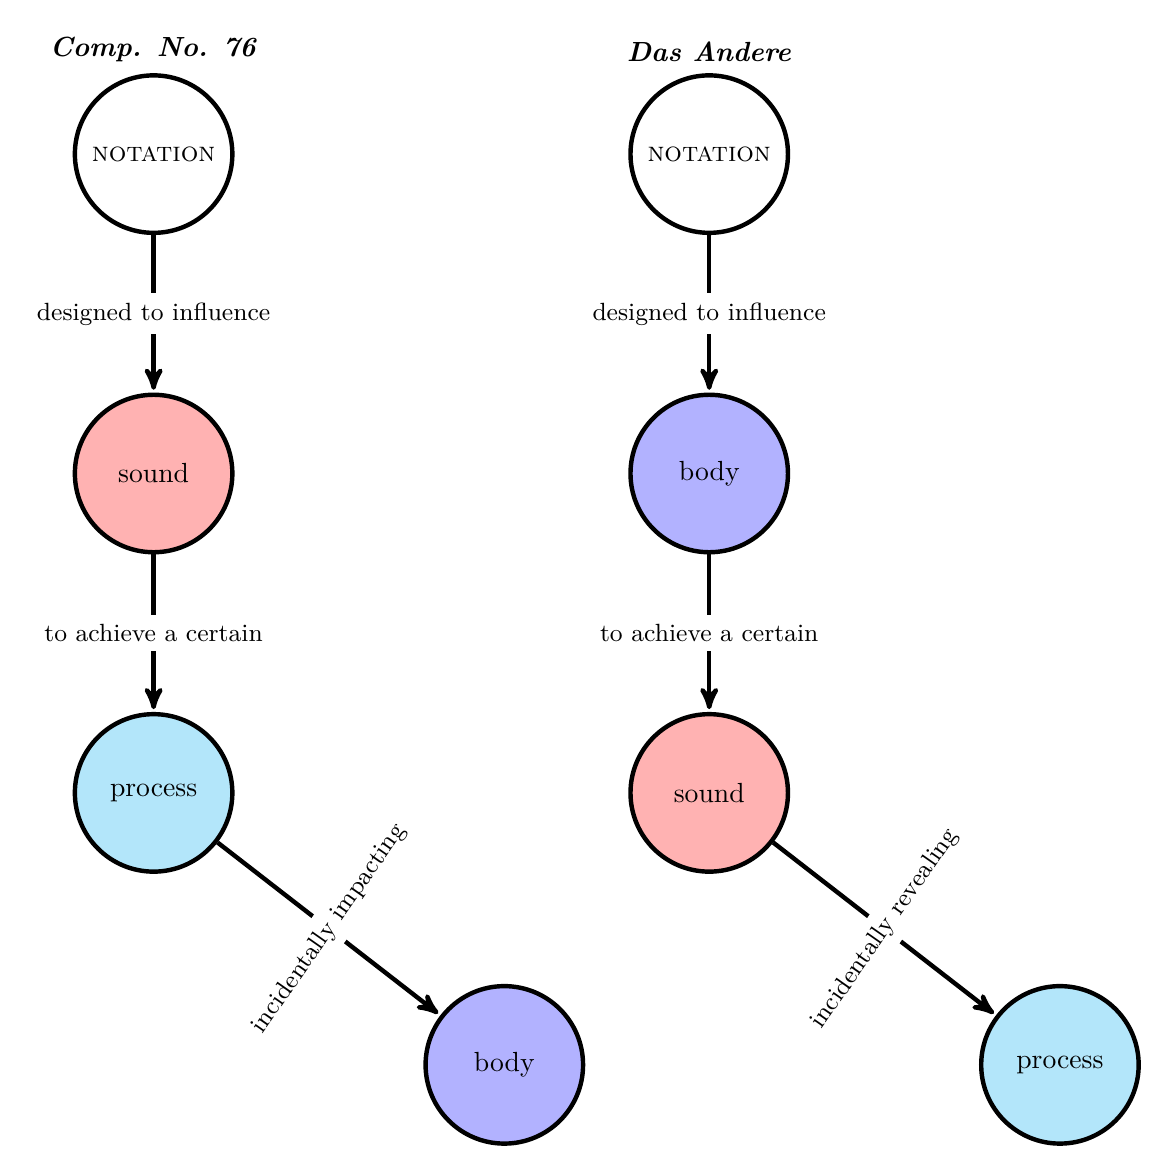
\begin{tikzpicture}[->,>=stealth',shorten >=1pt,auto,node distance=2cm,ultra 
                                    thick,main node/.style={circle,draw,minimum size=2cm}] %,font=\rmfamily\small\bfseries
                \node[main node, label=above:\textit{\textbf{Comp. No. 76}}] (a) {\textsc{notation}};
                \node[main node, fill=red!30] (b) [below = of a] {sound};
                \node[main node, fill=cyan!30] (c) [below = of b] {process};
                \node[main node, fill=blue!30] (d) [below right =2cm and 3cm of c] {body};
                \node[main node, label=above:\textbf{\textit{Das Andere}}] (e) [right =5cm of a] {\textsc{notation}};
                \node[main node, fill=blue!30] (f) [below = of e] {body};
                \node[main node, fill=red!30] (g) [below = of f] {sound};
                \node[main node, fill=cyan!30] (h) [below right =2cm and 3cm of g] {process};
                \path[every node/.style={font=\rmfamily\small}]
                (a) edge node [fill=white, anchor=center, pos=0.5] {designed to influence} (b)
                (b) edge node [fill=white, anchor=center, pos=0.5] {to achieve a certain} (c)
                (c) edge node [fill=white, anchor=center, pos=0.5, rotate=55] {incidentally impacting} (d)
                (e) edge node [fill=white, anchor=center, pos=0.5] {designed to influence} (f)
                (f) edge node [fill=white, anchor=center, pos=0.5] {to achieve a certain} (g)
                (g) edge node [fill=white, anchor=center, pos=0.5, rotate=55] {incidentally revealing} (h);
            \end{tikzpicture}
            }
        \captionsetup{width=.5\textwidth}
        \caption{Illustration of influence ``flow'' through \textit{Composition No. 76} and \textit{Das Andere}}
        \label{fig:flowdiagram}
    \end{figure}

    Of course, R\u{a}dulescu complicates this reading by expanding \textit{Das Andere}'s notation scheme to encompass a distinctly Braxtonian ``subjective interpretation'' during the construction of Op. 89. \textit{Das Andere}, written nine years prior, had already put forward a more-or-less complete vehicle for the creation of \textit{sound plasma} even without provisions for performer-mapped notational semantic content. Though the factors which transmuted body-data into ``precisely imprecise'' sound remained essentially unchanged between the two works, R\u{a}dulescu saw fit to expand the ritual function of the music---taking it from a mere downstream effect of the sound to an inseparable aspect of the act of performance itself. At this point it becomes particularly difficult to ignore the extent to which R\u{a}dulescu's three-axis interpretation rubric (Fig.~\ref{fig:radulescu_triaxial}) echoes Braxton's now-venerable Tri-Axial philosophy (for which his philosophical tract was named) which suffuses all aspects of his creative expression.\footnote{Unfortunately, this work lacks the space for a full (or even modest) rendering of the central tenets of Braxton's Tri-Axial philosophy. For now it must suffice to explain that Braxton conceives of his work as drawing together many crucial sets-of-threes: \textit{mutable}, \textit{stable}, and \textit{correspondence} logics (traditional improvisation, extant works, open works); ritual and performance logics of the past, present, and future; the \textit{primary}, \textit{secondary}, and \textit{tertiary} material of Ghost Trance Music; the three levels of inquiry used to construct the \textit{Tri-Axium Writings} (which are, of course, separate from the three central \textit{goals} of the \textit{T-AW}: \textit{affinity postulation}, \textit{axium correlation}, and \textit{reality imposition}). --- For more information, please see \shortcite{Braxton_1985}; \shortcite{Cauwenberghe_2021}; \shortcite{SA16}; \shortcite{Lock_1989}; \shortcite[167--75]{Lock_2000}; \shortcite{Lock_2008}}
    
    While the existence of a direct lineage between the two conceptual frameworks is unlikely, it seems noteworthy (to say the least!) that R\u{a}dulescu's effort to create new forms of notation (intended specifically to represent the music's ritual considerations) manifested itself in a three-dimensional structure directly homologous to Braxton's own tri-axial artwork-interpretation (etc.) scheme. In expanding \textit{Das Andere}'s notation to include Lao Tzu's sacred/secular text as well as an appropriate set of tools to bring it to bear on Op. 89's sonic materials, R\u{a}dulescu integrates multi-layered structures of denotative/connotative notational hybridity in much the same way Braxton had nearly two decades prior. Rather than interpret this change as a sudden realignment of R\u{a}dulescu's musical priorities, we might read the ``three-dimensionalization'' of the \textit{Das Andere} system not as a means of replacing but of \textit{reemphasizing} the music's spiritual component; an aspect already present but in danger of being lost if the work was only ever a series of micro-improvisatory physical gestures and the whirling, buzzing sound-world they produced. R\u{a}dulescu's music never sought to reach the same diversity of macro- and micro-level improvisatory play-environments that Braxton created in \textit{No. 76}. In deploying his unique mode of simultaneous hybridity, however, R\u{a}dulescu was able to, at least fractionally, allow his performers to play a collaborative role in ascertaining the shape and color of the \textit{sound plasma} ritual.
    
    \section{Conclusion}

    \textit{Prima facie}, the two compositional paradigms elaborated over the past fifty or so pages seem fairly similar. Both artists begin with essentially the same sorts of raw materials:

    \begin{smallquote}
    \begin{itemize}
        \item a foundation in traditional notation;
        \item a need to create a particular sort of indeterminate sound-world;
        \item a system of ``graphic'' open notation featuring...
        \begin{itemize}
            \item well-defined elements for inducing action and modifying that action and
            \item more vaguely-defined or un-defined elements requiring performer-mapping to function;
        \end{itemize}
        \item and a notational syntax which contextualizes these elements and allows their spatio-temporal deployment.
    \end{itemize}
    \end{smallquote}

    Further, both artists blend traditional and bespoke notations; making for a playing experience in which musicians must balance traditional notions of recitation with active creative decision-making through forms of improvisation. Readily apparent, however, to anyone with even a passing knowledge of these artists is that their compositional processes, their musical products, and their attendant philosophical frameworks differ wildly. The paradox articulated by this distinction---namely ``How do two work-complexes, both nominally neo-notational and improvisatory, wind up so vastly different?''---is one I hoped to begin answering in this chapter. Specifically, it has been my contention that more subtlety exists in the ways novel systems of notation are constructed and used than is typically addressed in scholarly literature. Deeper understanding of the ways that notation serves to mediate performance (and performer/composer agencies) demands a more thorough mode of interrogation---not only of general properties of notation systems (as we found in Ligeti's novel typology last chapter), but of the specific ways that new notations are lent meaning in the context of a musical work. 

    Braxton and R\u{a}dulescu strike me as two of our most fascinating systems-developers. Throughout their respective catalogues (though perhaps especially in the works mentioned here), both demonstrate dogged pursuit of (truly) radical musical ideals and both share an expertise in the way notation can be used to bring these ideals to bear for both performer and listener. I hope that this chapter has served not only as a justification for my admiration of these artists' working methods, but also as an elucidation of the ways notation's fundamental particles can dramatically influence compositional systems. I contend that only through a greater understanding of notation's general operating principles---e.g. through efforts like Ligeti's novel notation typology established last chapter---as well as close examination of these notational quanta, that we might more fully come to terms with notation's power and influence over the way we write and perform music.

    % \begin{notestuff}
    %     But in bringing them together and eschewing any one level of creative engagement with the written material, Braxton does something truly unique. His point is to explore human creativity in all of its forms and under all sorts of creative constraints; something none of his predecessors really accomplished. Notation is an excellent mechanism to achieve this.
    % \end{notestuff}

    % \begin{notestuff}
    %     Though 76 was written well before these ideas were cemented in prose, its score exemplifies the ideals of the Afrocentric orientation toward notation Braxton describes here. [then describe the process mentioned last paragraph as exemplifying this]
    % \end{notestuff}

    % \begin{notestuff}
    %     \begin{itemize}
    %         \item Braxton's context is one of improv-first. Everything is negotiable and subject to change according to (to use his term) the ``realness of the moment.''
    %         \item Rad's context is one in which undefineds or unknowns are typically critical errors---which demand immediate rectification lest the performance be less-than-complete or less-than-authentic.
    %         \item I am using the term ``connotative'' or ``performer-mapped'' to refer to anything that (GIVEN THE CONSTRAINTS LAID OUT IN THE SCORE) lacks well-defined semantic content granted by the composer. 
    %         \item There is a sense, though, in which (given the hyper-negotiable nature of the score) anything and everything is subject to change, to re-mapping at the performer's whim. 
    %         \item In this sense Braxton's ``hybridity'' is then, absolute, since nearly everything is both decisively denotative and apt to be re-mapped.
    %         \item Nevertheless, these works are now functionally autonomous. Contemporary performers who pick these works up and intend to perform them are not privy to the ``private details'' pertaining to notation interpretation which may have been known quantities in the work's initial context.
    %         \item Therefore we have no choice but to go ahead and treat the unknown and ill-defined elements as essentially open to performer-mapping; ergo a critical part of the structures of hybridity present in the work.
    %     \end{itemize}
    % \end{notestuff}

    % \paragraph{R\u{a}dulescu} While the subtlety with which R\u{a}dulescu traverses structures of indeterminacy is itself noteworthy, it is worth examining separately the way that un-coded, strictly connotative structures seep into his otherwise rigorous system. 



\chapter{\{O-G\}}
%\section{Introduction}

    This final chapter is intended to describe in some detail the compositional fruits borne of my time spent investigating novel systems of notation. During this project, work always proceeded on two fronts simultaneously: scholarly and creative efforts. As I began developing more robust notions of the syntactic and semantic structure of (open) notations found ``in the wild,'' I increasingly became aware of the subtle but powerful ability of new notations to mediate performance in ways typically closed off to traditional methodologies. As such, I began work on a rather humble framework oriented specifically toward corralling improvising musicians' musical expression with varying degrees of constraint; the ultimate goal being a robust and entirely well-defined scheme with which to play-test structures of fixity-traversal in real time. These creative efforts would culminate in a ``capstone'' concert of original works for a variety of ensembles; each work employing this novel notation scheme in one form or another. Thus, this chapter documents my experiences as a composer-cum-system-developer, beginning with my initial motivations and design concepts, continuing on to details pertaining to the actual structure of the system, and ending with a description and assessment of the capstone works followed by a final reflection evaluating the system's efficacy and future.

\section{Motivations and conception}
    \subsection{Formative experiences with open notation schemes}

    %There were, in essence, two catalysts which eventually led to the work as it exists in its current form; one a ``push'' and the other a ``pull.''
    Over my two years' time in the performance and literature MFA at Mills College (and during my tenure in Oakland thereafter), I was, on many occasions, called to perform by my colleagues and visiting composers. As I was known to be a musician nominally specializing in improvisation, the scores for which I was tapped almost without exception involved some degree of open notation in addition to traditionally-notated material. Given the diversity of composerly voices in the program, this openness took many different forms ranging from flexible, stripped-down traditional notation (à la Berio's \textit{Sequenza I} (1958) to text scores (à la Stockhausen's \textit{Aus den Sieben Tagen} (1968) or any number of Pauline Oliveros' works from the 1970s--1980s) to, of course, every conceivable type of ``graphic notation.'' The demands placed on these open notations and the goals they were intended to achieve also varied considerably. Composers I worked with sought free-floating Cagean ``aleatory,'' or the shifting densities of Lutosławskian ``stochasticism,'' or the virtuosity of some kind of post-post-bop ``open improvisation;'' each of which seemed to mandate an appropriate graphic trace distinct from our traditional \textit{lingua franca}. Very occasionally, the composer's sound- or process-concept for these open materials would be clear, well-communicated, and artfully and efficiently notated, making for fruitful and relatively painless rehearsals. Far more often, however, these sections (which, to be clear, formed the work's creative core and \textit{raison d'\^{e}tre}) would prove to be intractably difficult to get right, requiring hours of rehearsal, endless composer/performer back-and-forth and, in the worst of times, eleventh-hour rewrites to remove or ``fix'' (literally) the offending material. 
    
    Unfortunately, the extent to which a score was aesthetically interesting or visually expressive seemed inversely correlated with its ability to be successfully ``decoded'' and interpreted. In fact, ``decoded'' is a bit of a misnomer in that new glyphs, where they appeared, would be deployed intuitively; inconsistently---more according to aesthetic principles than musical or conceptual ones. Simply put, in the large majority of cases there was no encoding mechanism in play at all. A series of black dots on a blank field might serve as rather precise rhythmically-proportional notation invoking a precisely-calculated number of pitchless chirps; or, alternately, it might stand in for ametric staccato improvisation within a particular mode. Without a protracted impromptu Q-and-A session with the composer, it was wholly unclear which s/he meant. Problems, naturally, increased in severity as ensemble sizes increased. In the end these experiences became so much the norm that I began to view these notational experiments---especially the ``graphic'' ones---as a lost cause; techniques best replaced by judicious use of explanatory text.\footnote{This is, of course, not to paint every Millsian scored improvisation as irredeemably dire. A number of performances (particularly for small groups whose musicians already enjoyed a degree of familiarity) actually turned out quite well. Where successful rehearsals/performances did occur, however, they tended to be the function of generally pleasant and communicative composers---not said composers' notation design acumen.}

    % \begin{notestuff}
    %     Do I need to actually describe some hypothetical offending graphic scheme...? Visually-impressive but with milquetoast sounds? Barbed wire scores? Or something even more involved-looking but which amounted to chaotic swells? Especially a problem as ensemble size increased...
    %     There was a running joke... <>
    % \end{notestuff}
    
\subsection{Something better}

    % \begin{notestuff}
    %     \begin{itemize}
    %     \item Discovering Roscoe's and Braxton's successful experiments with open notations.
    %     \item Lamenting that I haven't had space to talk about Roscoe
    %     \item Excerpting L-R-G as protoypical successful open notation
    %     \end{itemize}    
    % \end{notestuff}

    Thankfully, while these lackluster firsthand impressions pushed me away from open scoring, I was fortunate enough to be pulled back in, obliquely, by a number of important influences. 

    \subsubsection{Roscoe Mitchell}
    Though I had always been particularly drawn to scores as art-objects and had dabbled to a degree with alternative notations, my time at Mills ultimately resulted in access and exposure to many more compositional paradigms than had been available to me prior. In particular, Roscoe Mitchell's composition lessons and group improvisation-sessions proved most valuable in this regard.\footnote{Lamentably, despite my abiding appreciation for Mitchell's works (both as bandleader/composer and with the Art Ensemble of Chicago) I lacked the space in Chapter Three to expand my discussion to these pieces. Mitchell's subtle, highly personal relationship to notation absolutely merits a detailed investigation of its own.} Prof. Mitchell's music had been an important factor in my decision to apply at Mills; since I became aware of his work, I had always been drawn not only to his acute blending of the cerebral and the brute, but also to the constant tension his work seemed to exhibit between clearly improvised material and material which could only have been orchestrated pre-performance. Though I did not know it at the time, Mitchell had developed (among other techniques) a number of simple but sophisticated ways of working with notation that facilitated this blend of fixed/open materials.
    
    Ultimately, my composition lessons granted me rare access to a number of Mitchell's unpublished scores; allowing me to come to grips with some of the ways this was accomplished over the years. Figure~\ref{fig:LRGexcerpt} illustrates an excerpt from one such score: \textit{L-R-G}; a trio for multi-instrumentalists originally written for Mitchell, Wadada Leo Smith, and George Lewis in 1978.  

    \begin{figure}
        \centering
        \fbox{\includegraphics[width=.9\textwidth]{images/chapter4/LRGpg3sys2.png}}
        \captionsetup{width=.5\textwidth}
        \caption{Excerpt from Roscoe Mitchell's \textit{L-R-G} (1978) (pg. 3, sys. 2) demonstrating simple, effective constraint over players' improvised gestures.}
        \label{fig:LRGexcerpt}
    \end{figure}

    \textit{L-R-G} represents a particularly seamless integration of familiar notation with improvisatory inducements of various types. When traditional notation appears, it is, in a sense, distilled to its (pitch + rhythm) essence---much in the same way as one might see in a typical lead sheet. It's clear from the outset that this is a system designed for the creative musician. Where improvisation is called for, it is induced by simple, bracketed portions of the staff---encompassing either the entire staff (as in Smith's first statement in Fig.~\ref{fig:LRGexcerpt}) or only part of it (Mitchell's gesture following the first four notes). Changes of instrument are called for (often in rapid succession) via capital-letter glyphs above the staff (\textit{A}lto \textit{S}ax, \textit{F}lute, \textit{P}ercussion for Mitchell here). Simple rules apply which render the fixed/open gradient transparent; facilitating not only reading but interacting \textit{via} reading. Mitchell demonstrated that meaningful improvisatory interaction could be scored---mediated---via graphic elements while still keeping interpretive ambiguity to a minimum. Indeterminate sound- or process-concepts could be encoded which were nevertheless concretely-defined and well-communicated. \textit{L-R-G}, along with its contemporary ``cousins'' \textit{The Maze} and \textit{S-II Examples} (which all appeared together on Mitchell's 1978 album concatenating the compositions' names) served, in a way, to indict the precious, over-wrought, but ultimately less-than-useful scores I'd experienced prior.\autocite{Mitchell_1978} The crucial difference seemed to be that the score itself served to establish clear rules constraining play; rules which, to be sure, were always fair game to break if need be, but which provided players a default set of parameters clearly communicating the composer's compositional aims.

    \subsubsection{Anthony Braxton}
    Likewise, though I was already a card-carrying Anthony Braxton devotee by the time I arrived at Mills, my time with Prof. James Fei (a long-time multi-wind player and Braxton collaborator) exposed me to far more---and more pertinent examples---of Braxton's music, as well as a greater understanding of his sometimes rather opaque working methods. Perhaps paradoxically, the most impactful of these systems was (and remains) Braxton's ``Language Music'' system. Generally, where the Language Musics are cited they appear as a list of twelve glyphs and the gestural families they represent (see Fig.~\ref{fig:language_types}). 

    \begin{figure}
        \centering
        \fbox{\includegraphics[width=.5\textwidth]{images/chapter4/anthony_braxton_language_types_2.jpg}}
        \captionsetup{width=.45\textwidth}
        \caption[Anthony Braxton's twelve ``language types'' which inform (among other things) his works for unaccompanied alto saxophone.]{Anthony Braxton's twelve ``language types'' which inform (among other things) his works for unaccompanied alto saxophone.\footnotemark}
        \label{fig:language_types}
    \end{figure}
        \footnotetext{\autocite{Lock_1989}}

    Despite all appearances, though, the twelve language types rarely if ever appear as such \textit{in situ}. Rather than representative glyphs to be used in scores, the language types are better thought of as bite-sized sound- and process-concepts which might be applied in any scored or improvised context. Most famously, they serve as the conceptual framework around which \textit{Composition No. 8A}--\textit{8G} were improvised on Braxton's seminal unaccompanied saxophone album, \textit{For Alto} (1969).\autocite[118--49]{Braxton_1988A} The mere fact that something as complex as constrained improvisation could be reduced to simple, two-dimensional glyphs and parametrized in terms of, say, duration and dynamic, again reinforced the notion that improvisers' creative potential could be meaningfully harnessed in the context of a scored work. Given that Braxton demonstrated that well-structured works could be composed using exclusively these gesture-zones (buttressed, of course, by the virtuosic efforts of a stellar improviser), it seemed a comparatively small leap to inscribe these zones on the page in the interest of composer-performer communication.

    Of course, (as demonstrated in the last chapter) not all of Braxton's notation schemata are so simple. Ghost Trance Music, in particular, which I began to study more closely around this time, served as a particularly fascinating example of integrative notation practices. Though the composition scheme would mutate considerably from its inception in the mid 1990s to its current form, Ghost Trance Music bears many consistent features across its instantiations.\autocite{Dicker_2016} Figure~\ref{fig:ghosttranceex} demonstrates two such features: 
    
    % \begin{figure}
    %     \centering
    %     \fbox{\includegraphics[width=.8\textwidth]{images/chapter4/361pg2sys1.png}}
    %     \fbox{\includegraphics[width=.8\textwidth]{images/chapter4/361secondary.png}}
    %     \captionsetup{width=.5\textwidth}
    %     \caption[Excerpts from fourth-species ``Accelerator Whip'' class Ghost Trance piece \textit{Composition No. 361} (2007) illustrating primary melody (above) and secondary material (below).]{Excerpts from fourth-species ``Accelerator Whip'' class Ghost Trance piece \textit{Composition No. 361} (2007) illustrating primary melody (above) and secondary material (below).\footnotemark}
    %     \label{fig:ghosttrance1}
    % \end{figure}
    %     \footnotetext{Score available thanks to Professor Fei's gracious loan.}

        \begin{figure}
            \centering
            \subfloat[\centering primary melody]
            {\fbox{\includegraphics[width=.7\textwidth]{images/chapter4/361pg2sys1.png}}}%
            
            \vspace{5pt}
            
            \subfloat[\centering secondary material]{\fbox{\includegraphics[width=.7\textwidth]{images/chapter4/361secondary.png}}}%
            \captionsetup{width=.5\textwidth}
            \caption[Excerpts from fourth-species ``Accelerator Whip'' class Ghost Trance piece \textit{Composition No. 361} (2007) illustrating primary melody (above) and secondary material (below).]{Excerpts from fourth-species ``Accelerator Whip'' class Ghost Trance piece \textit{Composition No. 361} (2007) illustrating primary melody (above) and secondary material (below).\footnotemark}%
            \label{fig:ghosttranceex}%
        \end{figure}
        \footnotetext{Score available courtesy of a gracious loan by Prof. Fei.---See \shortcite{Dicker_2016} for more details regarding the various Ghost Trance species and classes. }

    In the figure, (a) is a brief excerpt of the ``primary melody''---a long, unbroken melody which wends its way through the entire (often well over an hour long) composition. Where early Ghost Trance works often featured totally isochronous primary melodies sounding as a single, long line of quarter-notes, this late example obscures its primary melody almost entirely with ever-changing tuplets. Below (b) is the ``secondary material''---polyphonic music printed at the end of the score which serves as a reservoir into which performers might jump at particular times to be determined in-performance. Bracketing the minutiae of the system's organization (which deserve a dissertation all their own), I was taken, in particular, by the way Braxton was able to orient a composition around a fixed, unbroken melodic ``flow'' while at the same time building space for several levels of creative decision-making on the part of the performers (decisions which might equally validly be planned out on paper beforehand, hashed out in rehearsal, or arrived at spontaneously in performance).

    \subsubsection{George Lewis} 
    Though more limited, I would be remiss not to mention my experience with scholar-composer-performer George Lewis' early work as well. One piece in particular, \textit{Shadowgraph, 5} (for creative orchestra), which formed part of the curriculum in one of our large improvising ensembles, stood out as a particularly economical example of improviser mediation. Figure~\ref{fig:Shadowgraph} gives a single page for the ``saxophone'' group where Lewis combines textual directives, traditional (and modified-traditional) notation in varying degrees of openness, and a single bespoke glyph (the triangle) indicating unconstrained improvisation. Here I was drawn to the work's modularity and flexibility: the piece (like many of the AACM's scored works) is meant to function with an ensemble of any scale and may expand or contract to fit any desired duration. 
    
    Of particular note, though, is the emergent structure of the performer-score interaction. As players navigate the grid, the choice of which sub-module is selected for play is contingent not only on the operant rules-of-play, but also on a continuous stream of sonic and visual data from the rest of the ensemble. The function of the score is to delimit the player's creative choices to adjacent sub-modules while simultaneously demanding a meaningful and relevant contribution to the overall texture within those constraints---a mode of play which strikes me as, in a way, once-abstracted from lead-sheet interpretations. Rather than simply rhythmically or harmonically re-interpreting a lead-sheet symbol to suit the moment's demands, a player (at least in my experience with the work) sits in suspense waiting for the best possible moment to deploy one of the four adjacent sound-zones in their quiver; selecting not the \textit{right note} but the \textit{right mode of play} for a particular scenario. 

    \begin{figure}
        \centering
        \fbox{\includegraphics[width=.6\textwidth]{images/chapter4/shadowgraph.png}}
        \captionsetup{width=.5\textwidth}
        \caption[Excerpt (saxophone part) from George Lewis' \textit{Shadowgraph, 5} (1977).]{Excerpt (saxophone part) from George Lewis' \textit{Shadowgraph, 5} (1977).\footnotemark}
        \label{fig:Shadowgraph}
    \end{figure}
        \footnotetext{\autocite{Lewis_1977}}

    \subsubsection{The New York School}
    Of course my model frameworks extended beyond those of the AACM as well. The New York School, specifically, generally loomed large in the Millsian collective imaginary; both in terms of their theoretical output and their compositional methods. Thus it is no coincidence that in Chapter One I alotted significant space to the unpacking of several new notation methods developed in the 1950s and early 1960s by the likes of John Cage, Morton Feldman, and Earle Brown. Owing, I think, to their relative conceptual simplicity and their ease of adoption by diverse ensembles, New York School compositions repeatedly cropped up in and out of the classroom.

    These artists, steeped though they were in the literate Western art music tradition, treated the score not as a mere afterthought---as a brute archival necessity or a means of mechanically translating S/PC to sound---but as an art object in its own right. However, this focus on the visual never compromised the scores' function \textit{as scores}. Often (excepting, perhaps, the wilder of Cage's scores) golden-era New York School compositions seemed to adopt a Bauhausian functional aesthetic that reduced the notation's inducements and modifiers to their bare essentials: a rectangle for an instrument's functional range; a dot or a line for an inducement to act; its length or breadth a modifier. These were scores which could, in the span of an hour, be picked up and played with little ambiguity as to what, conceptually, the composer was seeking. Figure~\ref{fig:NYS} is a small, semi-representative sampling of these scores' plain, economical visual traces.
    
    \begin{figure}
        \centering
        \subcaptionbox{Cage---\textit{Aria} \label{fig:cage}}
            {\fbox{\includegraphics[width=.3\textwidth]{images/chapter4/cage_aria.png}}}
        \subcaptionbox{Wolff---\textit{Edges} \label{fig:wolff}}
            {\fbox{\includegraphics[width=.4\textwidth]{images/chapter4/wolff_edges.png}}}

        \vspace{7pt}
            
        \subcaptionbox{Feldman---\textit{Projection 1} \label{fig:feldman}}
            {\fbox{\includegraphics[width=.3\textwidth]{images/chapter4/feldman_projection_1.png}}}
        \subcaptionbox{Brown---\textit{Four Systems} \label{fig:brown}}
            {\fbox{\includegraphics[width=.4\textwidth]{images/chapter4/earle_brown_four_systems.png}}}
        \captionsetup{width=.5\linewidth}
        \caption[(Brief!) excerpts from four semi-representative ``New York School'' compositions demonstrating minimal, comprehensible open notations.]{(Brief!) excerpts from four semi-representative ``New York School'' compositions demonstrating minimal, comprehensible open notations.\footnotemark}
        \label{fig:NYS}
    \end{figure}
    \footnotetext{(a) \autocite{Cage_1958}; (b) \autocite{Wolff_1968}; (c) \autocite{Feldman_1964}; (d) \autocite{Brown_1986}}

    \subsubsection{The lead sheet}
    
    Certainly not least among my influences pertaining to this research was my time spent (in various scenes and with varying degrees of dilletantism) as a jazz horn player, guitarist, and drummer. As discussed at some length in earlier chapters, the relationship between jazz performance practice and musical literacy is a complex one. However, it should be safe to claim, at the very least, that the lead sheet model of composition has since the 1940s at latest been the \textit{de facto} standard means of inscribing jazz compositions for easier play, distribution, and archiving (Goodwin's ``TuneDex'' having been introduced in 1942).\footnote{See Ch. 1, ``The Afro-diasporic return to open notation''---\autocite[]{Abel_2016}} As a musician who, for better or worse, has been concerned more with \textit{breadth} of understanding of a given corpus than \textit{depth}, I have typically relied on lead sheets for rehearsal and performance much more than musicians who routinely commit tunes to memory. As such, over the years I slowly became aware of the potent ways the lead sheet's stripped-down glyphs might impact improvised performances. Changing a simple E$\flat^{7}$ glyph into an E$\flat^{7(\flat 9 \sharp 9 \flat 13)}$ has the potential to radically rewrite the field of potential action afforded to a player at a particular point in the composition. (For visual reference, Figure~\ref{fig:monk} provides one such lead sheet: an original manuscript of Thelonious Monk's evergreen ``Monk's Mood'' with the melody evidently transposed for a B$\flat$ instrument.)

    \begin{figure}
        \centering
        \fbox{\includegraphics[width=.63\textwidth]{images/chapter4/monk_manuscript_monks_mood.jpg}}
        \captionsetup{width=.5\textwidth}
        \caption[Original manuscript of Thelonious Monk's ``Monk's Mood''. Melody transposed for B$\flat$ instrument.]{Original manuscript of Thelonious Monk's ``Monk's Mood''. Melody transposed for B$\flat$ instrument.\footnotemark}
        \label{fig:monk}
    \end{figure}
        \footnotetext{Sold at Bonhams, 16 June 2015 for \$20,000!---\autocite{Bonhams}}

     Lead sheets, after all, represent far and away the most common means of invoking and shaping a collective, creatively-constrained improvisation of any sort. Here as elsewhere, the score does not function as a complete system-unto-itself, instead relying rather heavily on syntactic and semantic standards which musicians must slowly accrue over the course of an entire musical career. However, for those already inducted into the system, the lead sheet (despite typically lacking the usual trappings of traditional scores---dynamics, expressive text, articulations, etc.) bears great power to influence precisely how players approach a tune. This provides an important object-lesson for the would-be notation designer. Namely: the clarity and efficiency with which a notation scheme is able to communicate is often contingent on factors external to the text---specifically the ways in which its users develop a working understanding of its use.

\section{Designing a system}

    Having been exposed to so many laudable methods of writing for improvisers, it became apparent (sometime circa 2020) that the best way to ameliorate the problems I'd faced was (despite all attendant risks) to start work on my own humble notation scheme; ideally aggregating the best attributes of the above (pseudo-)systems while avoiding the pitfalls of haphazardly-constructed one-off ``graphic'' scores. The following section will describe the process by which I designed and implemented such a system. While I'll spare the reader an exhaustive enumeration of each relevant or marginally interesting detail, I will take care to point out particularly thorny or illuminating problems which cropped up along the way.

    This system would be organized around a rather abstract central conceit: that of a sort of ``subtractive'' composition. Traditional notation on the whole might be thought of as a sort of coordinate system which, at its empty ``rest state'' (i.e. a blank score) denotes the musical null set (\O); silence; no play. As symbols are added to the empty canvas of the score, play is induced. A single note represents a single attack with various parameters. Traditional notation is, after all, a system which from its outset (despite its many open forms) was used less for novel creation than for reproduction. If instead we desire the opposite---a system which privileges openness over fixity and production over reproduction---we must begin from the polar opposite standpoint. That is to say: the ``rest state'' of a notation for improvisers should denote the universal set---the set of all possible utterances. For a musician presented with a blank page, all is permitted; the composition denotes no boundaries. The job of our library of symbols, then, must be to pare down this universal set of utterances into a set of potential actions which befits the composer's sound- or process-concept. Here, an action is not built up from silence, but is arrived at through gradual restriction of possible musical moves. The clear analogy here is to two antipodal methods of sculpting. Where the model-maker builds via accretion, slowly adding bits of clay to a form until it eventually resembles some initial work-concept, the stone-carver visualizes a form trapped in the block of alabaster---the set-of-all-forms---freeing it by chipping away unwanted material.

    In truth, not much changes in terms of practical compositional procedure under such a scheme: a composer still selects symbols for interpretation according to some desired sonic or gestural outcome and a performer still interprets them, producing sound. Given, however, that the notation is now organized entirely around varying degrees of variability/indeterminacy, we should expect that such a system should facilitate more complex and interesting forms of open music-making. 

\subsection{Design desiderata}

     Work was quite nebulous to begin with; amounting essentially to a small but growing list of desiderata. The following (presented in loose order of priority) constitute the various ``non-negotiables'' which I saw from the outset as particularly crucial to a functioning notation-for-improvisers.
    
    \begin{enumerate}[label=(\roman*)]
        \item \textit{The system should comprise entirely well-defined glyphs.} Given that the idea to develop a notation scheme in the first place was catalyzed by general dissatisfaction with vaguely- or undefined quasi-symbols, it was critical from the very beginning that each symbol be well-defined and behave identically across instances in a score (or across several scores).\footnote{Again, this is not to somehow denigrate partially or purely-connotative notations which (as I hope Chapter Three has illustrated) can themselves give rise to great art---these are simply the initial boundaries set for the project.}

        \item \textit{The system should adequately balance broad range of potential sonic
        territory with symbolic economy.}   As Pierre Boulez noted in a Coll\`{e}ge de France lecture, 

        \begin{smallquote}
            In the case of known, familiar objects [...] with universal conventions, transcription is a simple matter, but runs the risk of influencing ideas to ensure that they can be included in a familiar mould without special problems. With new objects [...] whose codes are presently uncertain, even non-existent, transcription becomes difficult, imprecise, exaggeratedly complex – complex to the point of uselessness – because one no longer knows how to connect an over-elaborate notation to the object in question. The problem lies in the attention required by the signs defining the object that one wants to communicate – quantitative or qualitative.\autocite[532]{Boulez_Nattiez_2019}
        \end{smallquote}

        \noindent In short, a system of signs is only as good as its ability to be decoded in the context for which it was designed. A system which over-multiplies its symbols in the name of ever-greater representative power runs the risk of requiring too much effort---cognitive, in this case---to decode. On the other hand, a system which is overly-stripped-down in the name of ``readability'' runs the risk of constraining that which it hopes to represent to too great a degree. Thus, any sufficiently mature notation scheme should be able to fluidly negotiate these two factors.

        \item \textit{The system should function equally as a means of transcription as well as performance.}   One of the many strengths of traditional notation is its translational bi-directionality. That is: traditional notation is structured such that a page of well-organized symbols may be realized in sound, but equally that instrumental utterances may be usefully encoded in symbols directly with minimal signal degradation. In other words, a unit of notation's resultant sound is sufficiently tightly-coupled to an instance of a particular symbol that a listener may robustly re-encode a composition from sound alone. This fundamental attribute of the system allows music to be transmitted not only page-to-musician, but musician-to-page. Of course, being that my desired system would deal primarily in variously-constrained improvisation with indeterminate sonic results, it would always demonstrate a lower (read: noisier) signal-to-noise ratio. However, if designed adequately, the system should permit a musician to create a reasonably high-fidelity transcription of an improvisation which otherwise would be quite difficult to represent using traditional notation.\footnote{
            To be clear, the desires for my project differed from those realized in Andrew Killick's ``Global Notation.'' Where his system tailors the notation's encoding methodology to the needs of whatever musical practice is under scrutiny, my transcriptions would always be once-abstracted approximations prioritizing larger-scale clusters of gestures. That said, Global Notation represents a fascinating attempt at solving a centuries-old problem. Because different musical communities build their work-concepts from very different constitutive elements, transcribing a work in Global Notation necessarily involves considering multiple degrees of gestural fixity depending on whether the instrument/practice in question values rhythm over pitch; duration over meter; dynamic over timbre; etc. To that end, for any given instrument it provides a robust means of representing open vs. fixed pitch, open vs. fixed rhythm, and so on. For more information on the motivation behind and use of Global Notation, please see Killick's website.---\autocite{Killick}.
        }
        
        \item \textit{The system should be easily integrated with traditional notation.} Rather than quixotically attempt to replace or subvert traditional notation, I thought it best to incorporate its strengths (not to mention musicians' existing musical literacy) into the new scheme. Thus, the system ought to allow any new glyphs to ``slot in'' alongside more familiar symbols.
        
        \item \textit{The system should be reasonably intuitive to new adopters and sight-readable with minimal effort.} Traditional notation features a number of root-level attributes which persist across nearly all of its instances: regular mapping of time and pitch to $x$- and $y$-axes; left-to-right and top-to-bottom read order; inducement-and-modifier pairings, etc. A new notation scheme ought to preserve these foundational principles so as to facilitate integration with traditional notation and avoid unnecessarily bewildering the reader. 
        
        % \item \textit{The system should be sight-readable with just a little practice.}   Given typical real-world constraints on improvising ensembles (read: limited resources; scant rehearsal time), an over-complicated system requiring constant reference to tables, figures, or other literature would only hamstring performance.
        
        \item \textit{The system should be useful without a strong background in traditional Western musical literacy.} As any sufficiently-experienced musician will tell you, virtuosic talent for improvisation does not always coincide with traditional musical literacy. A successful notation scheme for improvisers, then, should remain accessible even to those ill-versed in Western notation. That is to say: one ought to be able to construct well-formed scores entirely within the system itself.
        
        \item \textit{The system should be easily renderable using pen-and-ink on paper.} Given the utter ubiquity of electronic devices which can engrave or copy arbitrarily complex notation, this bullet point might betray my own aesthetic preferences more than it describes a non-negotiable attribute for a notation scheme. That said, it is unquestionably a boon to be able to quickly jot down an imagined sound-concept or overheard gesture without needing to resort to, say, iPad-specific software or a 3-D rendering engine.
        
    \end{enumerate}

    Armed with these design constraints, I began by narrowing down (a) the parameters I would seek to encode and (b) the visual trace of the notation which would eventually encode them. Initially I imagined the sorts of parameters I would (consciously or unconsciously) consider if I were tasked with ``freely'' improvising in the context of a composition: Would it be rhythmic or arrhythmic? Played with a noisy or pure tone? Involving some sort of imposed tonality or freely atonal? I found it helpful to visualize these parameters as a virtual bank of sliders which might be freely tweaked to suit the composer's desires. For a given gesture, these virtual sliders could either be held constant or varied. The presence of a slider in a particular position meant that its parameter was fixed, i.e. specified by the composer. Its absence would conversely denote an open parameter---one whose state at any given point would be determined by the performer. The notation's semantic fixity would therefore be continuously variable depending on the specificity of the encoding glyph(s). Figure~\ref{fig:sliders} illustrates four hypothetical positions of these imagined sliders which each represent a possible gesture. If it was to be considered a success, the notation scheme would need to be able to represent each gesture distinctly (i.e., either with all parameters fixed in a particular position or with certain parameters fixed and others open) and clearly communicate their relative openness or fixity at a glance.
    
    %Whichever form the notation was to take, it should be able to efficiently encode each parameter given here with enough degrees of freedom to illustrate their change over time (or their absence).

        \begin{figure}
        \centering
        \singlespacing
            \begin{tabular}{|r c l|}
                \hline
                irregular & \texttt{-----|-----------} & isochronous  \\
                noise & \texttt{--------|--------} & sinusoidal \\
                percussive & \texttt{--------------|--} & legato \\
                free atonal & \texttt{--|--------------} & scalar \\
                \lilyDynamics{pppp} & \texttt{--|--------------} & $\lilyDynamics{ffff}$ \\
                romantico & \texttt{-----|-----------} & meccanico \\
                high range & \texttt{---------|-------} & low range \\
                \hline
            \end{tabular}
        
            \vspace{7pt}
        
            \begin{tabular}{|r c l|}
                \hline
                irregular & \texttt{--------------|--} & isochronous  \\
                noise & \texttt{--|--------------} & sinusoidal \\
                percussive & \texttt{--|--------------} & legato \\
                \lilyDynamics{pppp} & \texttt{-----------|-----} & $\lilyDynamics{ffff}$ \\
                high range & \texttt{--------------|--} & low range \\
                \hline
            \end{tabular}
        
            \vspace{7pt}
        
            \begin{tabular}{|r c l|}
                \hline
                irregular & \texttt{--------------|--} & isochronous  \\
                percussive & \texttt{--|--------------} & legato \\
                high range & \texttt{--|--------------} & low range \\
                \hline
            \end{tabular}
        
            \vspace{7pt}
        
            \begin{tabular}{|r c l|}
                \hline
                free atonal & \texttt{--------------|--} & scalar \\
                romantico & \texttt{--|--------------} & meccanico \\
                \hline
            \end{tabular}
        
        \captionsetup{width=.5\textwidth}
        \caption{Four hypothetical parametric configurations for gestures ideally renderable in this as-yet-unnamed notation scheme, from most fixed (top) to most open (bottom).}
        \label{fig:sliders}
        \end{figure}

    The second primary consideration was the form of the graphic elements themselves. Given that these would serve as the tools by which gestures would be encoded as well as an interface for composer/performer communication, it was crucial that their design be well-motivated. From the very start I was particularly drawn to elegance and economy of Braxton's twelve ``language types.'' Although that they were never meant to serve as notation as such, I admired their easy readability, their modularity, and their distinctive, stripped-down aesthetic. While the aforementioned twelve are the most frequently cited and reproduced of Braxton's categories of sound, a cursory glance at the introduction to any of the four volumes of his \textit{Composition Notes} yields a treasure-trove of glyphs and the sound classifications they represent. Figure~\ref{fig:soundclassifications} gives a small sampling of these additional sound classifications not present in the initial twelve. Again, one is unlikely to see these glyphs serving as notation proper while poring over the excerpted compositions themselves. For Braxton, they instead primarily serve to reify a particular S/PC in an quickly-referenceable form---acting more as a mental library of techniques to be deployed in composition in other forms. Like the original twelve language types, though, they provide an excellent model for the notation-designer seeking recognizable, easily-reproducible graphic forms with a high degree of representative power.

        \begin{figure}
        \centering
        \fbox{\includegraphics[width=.45\textwidth]{images/chapter4/braxton_supp_1.png}}
        \captionsetup{width=.5\textwidth}
        \caption[A sampling of additional ``Sound Classifications'' from Braxton's \textit{Composition Notes}.]{A sampling of additional ``Sound Classifications'' from Braxton's \textit{Composition Notes}.\footnotemark}
        \label{fig:soundclassifications}
    \end{figure}
        \footnotetext{\autocite[v-x]{Braxton_1988}.}


    \subsection{Early efforts}

    \subsubsection{Graphic structure}
    My first exercise as fledgling architect, then, was to consider how to represent the twelve language types in my own notation (by now having been given the working moniker ``Otto-Glyphs''---\{O-G\}) such that they might move beyond mere conceptual stand-ins for sounds.\footnote{Please forgive the typographical flourish. Given that ``ogee'' is a term of art referring to serpentine curves (especially in architecture) I couldn't resist the temptation to incorporate curved brackets (comprising four ogees total) in the abbreviated name of the system.} Figure~\ref{fig:braxtonlike2} gives an early sketch of this process. From quite early on, I wanted a way to illustrate both \textit{global parameters} (which would apply across the entire modular gesture) and \textit{local parameters} which might change over its course. As such I opted for an expanded version of Braxton's ``head-and-tail'' format where the ``head'' (the square in Fig.~\ref{fig:braxtonlike2}) initiates the gesture and contains information relating to global parameters and the ``tail'' (the glyphs which follow the head) show its duration and give changing local parameters. Global parameters here might take the form of a key or tonality (B$\flat^{\triangle}$, VII, etc., in Fig.~\ref{fig:braxtonlike2}) or a technique (growling, sul pont.) and be expressed via text or common symbol in the ``box.'' Local parameters (approximate pitch height, dynamic, attack envelope, silence) would be encoded directly in the ``tail'' itself via a combination of $x$- and $y$- coordinates, stroke weight, and empty space.

        \begin{figure}
            \centering
            \fbox{\includegraphics[width=.65\textwidth]{images/chapter4/braxton-like-1.png}}
            \fbox{\includegraphics[width=.65\textwidth]{images/chapter4/braxton-like-2.png}}
            \captionsetup{width=.5\textwidth} 
            \caption{An early attempt to render Braxton's twelve ``language types'' into \{O-G\}.}
            \label{fig:braxtonlike2}
        \end{figure}

    \subsubsection{Brackets}
    This exercise alone gave enough shape to \{O-G\} that I could begin experimenting with short scores comprising these types of gestures---leading rather quickly to some key expansions of the system. From the outset, \{O-G\} was conceived as a means of more finely controlling notational semantic fixity---of providing greater or lesser degrees of informational specificity to a performer. What it so far lacked, however, was a way of efficiently communicating rapid, radical changes to this fixity. As we saw in Chapter Three, \textit{Composition No. 76} provided its performers with clear boundaries between gestures which are to be performed (at least loosely) as-written and those which are to form the basis for a more radical form of creative contribution. To achieve a similar clarity, I began to incorporate bracket notation akin to the type used in \textit{L-R-G}. An empty space on the score wrapped by square brackets would denote the aforementioned ``universal set'' of improvisatory gestures---i.e. the direction to ``freely improvise.'' The creative potential for a fixed/open ``on/off'' switch could exceed this simple binary, though. Here I'll quote directly from the user's manual (to be discussed in further detail later in this chapter).

    \begin{smallquote}
            In essence: any time brackets appear, they should be read as: \textbf{play something \textit{in this manner}}. How precisely \textbf{\textit{in this manner}} is interpreted will of course differ greatly between performers. For instance: Where this figure...

            \begin{center}
            \includegraphics[width=.2\textwidth]{images/chapter4/01-3dotscurve.png}
            \end{center}
            
            \noindent indicates \textit{three short attacks and a brief legato passage} across a particular duration, its bracketed counterpart

            \begin{center}
            \includegraphics[width=.2\textwidth]{images/chapter4/01-3dotscurvebracket2.png}
            \end{center}
            
            \noindent asks the performer to play using these \textit{sorts of} gestures for the duration indicated by the brackets/arrows. Rather than specify certain sounds in certain orders, the bracketed gesture gives a player a sort of ``sonic territory'' to occupy for a given time. The player ought to feel more ``freedom'' with respect to the execution of the material therein than with the more cut-and-dry plain gestures.\footnote{\textit{Otto-Glyphs}, pg. 19--20, Appendix}
    \end{smallquote}

    To my mind, incorporating this ``rapid-traversal'' mechanism would both (a) provide the player with a visual cue to quickly reconsider the way a certain gesture might fit into the prevailing texture and (b) grant them the creative liberty to reshape the components of that gesture to suit the moment's needs.

    \subsubsection{Relational parameters}
    Another key development which followed initial experiments was the development of signs for cuing and other relational parameters. Braxton's relational codes (as referenced in Chapter Three---\textsc{dom}, \textsc{supp}, \textsc{op}) provided a simple working model for how these might be deployed. It seemed intuitive, though, that these codes might be expanded to allow more a more fine-grained shaping of these inter-musician relationships. By default, any performance practice for which improvisation is a central organizing factor sets up listening-response feedback loops between its performers. Instituting these relational parameters, though, allows this feedback itself to serve as a locus of creativity in a way that is typically inaccessible to composers.

    By far, the best examples of fine-grained relational composition come in the form of conducted improvisations---namely Butch Morris' ``Conduction'' system and Walter Thompson's ``Soundpainting.'' Since I unfortunately lack the space or time to expound in any great depth on the fascinating living notation which forms these systems' foundation, it must suffice for now to briefly touch on the ways they impacted the early development of \{O-G\}. Admittedly, my firsthand experience with Conduction and Soundpainting was limited to strictly unofficial exercises---sometimes in accordance with the letter of the official manuals and other times in a sort of unholy amalgam of the two systems. Regardless, it is a testament to the efficacy of systems like these that even watered-down or corrupted versions may serve to meaningfully sculpt six, twelve, or thirty improvisers' creative output---even ones with wide variance in level of expertise, reading ability, experience with they system, experience improvising, etc. Despite the fact that the systems differ greatly in terms of central motivating ethos, both systems share general encoding principles: some central organizer (conductor or Soundpainter) incites and modifies gestures elicited from a player or group of players. The conductor then deploys a series of hand- and body-gestures, drawn from a symbolic library of such gestures made known to performers beforehand. Like other forms of notation, these composer-gestures comprise inducements which call for some sounding and modifiers which manipulate the performers' gestural parameters. As improv-centric systems, composer-gestures tend to be oriented toward creative constraint of players' actions---calling for open improvisation which is somehow pared down according to an intended dynamic, tempo, technique, etc. However, both systems feature codes which allow for quite precise inducements, even allowing encoding of precise melodic and rhythmic elements; practically on the order of traditional notation (though, admittedly this represents a comparatively rare use-case).\footnote{\autocite{Morris_2017} and \autocite{Thompson_2006_1}.}

    Naturally, the ``conductive arts'' differ from traditional scoring methods insofar as they allow continuous, live interplay between the players' sound-producing gestures and the conductor's gesture-producing gestures. This allows for compositions comprising pre-planned sequences of signs to be radically altered or abandoned all together if desired. Nevertheless, I came to think of \{O-G\} as a sort of flattened, concretized form of (small-c) conduction. Walter Thompson, in the first of a series of workbooks, lays out the component-level structure of Soundpainting thus:

    \begin{smallquote}
        The 43 gestures in Soundpainting Workbook I fall under 2 general categories: Sculpting gestures and Function signals.

        \vspace{7pt}
        
        \noindent Sculpting gestures indicate \textit{What} type of improvisation and \textit{How} it is to be performed, and Function signals indicate \textit{Who} performs and \textit{When} to begin performing.

        \vspace{7pt}
    
        \noindent \textit{Who}, \textit{What}, \textit{How}, and \textit{When} comprise the Soundpainting syntax. [...] 

        \vspace{7pt}
        
        \noindent The Soundpainting syntax is further broken down into 6 parts:
            \begin{enumerate}
                \item Identifiers (\textit{Who} is performing)
                \item Content (\textit{What} type of improvisation)
                \item Modifiers (\textit{How} to perform the improvisation)
                \item Go gestures (\textit{When} to begin performing)
                \item Modes (a set of parameters affecting specific gestures)
                \item Palettes (sections of notated or rehearsed music, text, choreography, or visual design)\autocite[4]{Thompson_2006_1}
            \end{enumerate}
    \end{smallquote}

    The workbooks go on to provide dozens of directives, denoting a wide range of performer actions from very simple, sound-oriented gestures (``long tone,'' ``hit'') to much more complex ones which actively modulate the degree of performer interactivity in performance. The ``shapeline'' gesture, for instance, requires that performer ``musically perform the physical shape the Soundpainter creates with her/his body---physical graphic notation'' where the ``synchronize'' gesture asks a performer to ``[synchronize] specified material with specific performer(s).\autocite[34--5]{Thompson_2006_1} Again, bracketing \textit{live} composer interactivity, it was my hope that \{O-G\} could function much in the same way. Systems were already in place which allowed for a parallel ``\textit{Who}, \textit{What}, \textit{How}, \textit{When}'' organizational structure. ``\textit{Who}'' and ``\textit{When}'' are handled in the same way as traditional notation: by position and alignment on the page. ``\textit{What}'' and ``\textit{How}'' are accomplished by conceptually transposing the four-dimensional movements of a conductor into two dimensional black-and-white glyphs. At this point, \{O-G\} only needed more refined ways of establishing and modifying performer-to-performer and performer-to-notation relationships. Figure~\ref{fig:relational1} illustrates an early attempt to workshop these signs and Figure~\ref{fig:relational2} shows their current form as of time of writing. Here, ``match,'' ``build upon,'' ``echo,'' ``memorize,'' ``recall'' signs in particular were borrowed from my experience with conduction, while ``dominate'' and ``support'' refer directly to the aforementioned \textit{Composition No. 76}.

        \begin{figure}
            \centering
            \fbox{\includegraphics[width=.9\textwidth]{images/chapter4/relationalcombine.jpg}}
            \captionsetup{width=.5\textwidth} 
            \caption{Workshopping relational glyphs.}
            \label{fig:relational1}
        \end{figure}

        \begin{figure}
            \centering
            \fbox{\includegraphics[width=.65\textwidth]{images/chapter4/relationaltable.png}}
            \captionsetup{width=.5\textwidth} 
            \caption{Relational glyphs: current form.}
            \label{fig:relational2}
        \end{figure}


    % \begin{notestuff}
    %     Segue to first composition
    % \end{notestuff}

    \subsection{\textit{Device for Encouragement of Applause}}

    By this point, with the system having grown to include a basic inducements-and-modifier structure, a means of subtly or radically modulating notational fixity, elements allowing cuing and modification of relational parameters, and now a growing library of basic symbols, the time had come to put the notation scheme into practice. The opportunity to do so arose in 2021 when I was tasked with composing a short (ca. five minute) new work for a mixed ensemble drawn from UC Irvine's ICIT\footnote{Integrated Composition, Improvisation and Technology.} and other music department graduate students.

    The basic theme of the work was the concatenation of two distinct, non-interactive modes of play in a background-and-foreground arrangement. The background---intended to recall a kind of Satiean ``furniture music''---comprised bass clarinet, 'cello, and flute reading from a more-or-less traditional score (Score A) on one extreme end of the performance space.\footnote{In performance: Isaac Otto---bass clarinet, Bella Pepke---'cello, Rebecca Larkin---flute.} Players of Score A self-pace a slowly-pulsed pad of clusters drawn (intuitively, essentially) from an evocative pitch-class set \{0, 2, 3, 4, 6, 7, 9, T, E\} (Messiaen's third mode of limited transposition) which was used as a harmonic reservoir. This pad texture was to loop unobtrusively behind the foreground for the composition's duration. Figure~\ref{fig:encouragementA} gives a one-system excerpt of Score A illustrating a type of proportional notation. Durations of tones and silences are determined by the `cellist's cues.

    \begin{figure}
        \centering
        \fbox{\includegraphics[width=.95\textwidth]{images/chapter4/deviceAsys1.png}}
        \captionsetup{width=.5\textwidth}
        \caption{\textit{Device for Encouragement of Applause}---Score A: System 1.}
        \label{fig:encouragementA}
    \end{figure}
    
    The foreground, on the other hand (Score B) was made up of an improvising duo on trap set and contrabass (located at the opposite end of the space).\footnote{In performance: Steven Lewis---trap set, James Ilgenfritz---contrabass.} Acoustically, I intended that Score B would evoke a chattering, unstable conversation; replete with unexpected, short shouts and frightened murmuring in response. Where Score A would swell and ebb in unison with only the barest inter-musician communication in the form of cuing nods, Score B was to feel more chaotically interactive.
    
    Gestures for the duo were also fully-notated---only now entirely in \{O-G\}. As this was to be the system's maiden voyage, I took care to to limit Score B's vocabulary to only a few distinct types of gestures. This way, I would be able to focus my efforts on assessing and fine-tuning the ways players interacted with the notation rather than on coaching performers on dozens more unfamiliar glyphs. Unlike Score A, which was entirely ensemble-paced, Score B featured no repeats and was paced by stopwatch, reducing the potential cognitive load on relying exclusively on intra-ensemble cues for pacing. Figure~\ref{fig:encouragementB} gives the first page of Score B illustrating this reduced feature-set. Of particular note is the occasionally extreme rate at which the duo here were required to re-assess (consciously or unconsciously) the openness of a given gesture. From the 1'30'' mark to around 2'15'', the bassist must perform two ``in this manner'' gestures (in semi-metronomic time) followed by fixed low tones interrupted by a harmonic---then must execute an open segement with overpressure, a fixed glissando upward, another open segment, and a fixed quiet \textit{col legno battuto} gesture all within the span of around thirty seconds (see Figure~\ref{fig:encouragementB}). While this is not a particularly onerous passage technique-wise, this rapid oscillation between fixed and open modes of play requires a constant renegotiation of one's relationship to the notated material itself (and therefore to the letter and spirit of the composition) as well as to one's bandmates.
    
    \begin{figure}
        \centering
        \fbox{\includegraphics[width=1.3\textwidth,angle=270]{images/chapter4/deviceBpg1.png}}
        \captionsetup{width=.5\textwidth}
        \caption{\textit{Device for Encouragement of Applause}---Score B: Systems 1--3.}
        \label{fig:encouragementB}
    \end{figure}

    %\subsubsection{Results}
    One key issue which arose during the composition process was that of instrument-specific glyphs. Having primarily performed as a woodwind player for the last decade or so, and having been initially inspired by Anthony Braxton's aforementioned language types (themselves designed around unaccompanied saxophone improvisation), I perhaps inadvertently designed \{O-G\} such that its structure demonstrates a prejudice for pitched, monophonic instruments or at least for gestures which behave monophonically. The fundamental units of notation here are dots (indicating short attacks), lines, and curves (indicating longer attacks undergoing some sort of flux). This did not pose a problem in particular for the bassist here, whose prescribed gestures do not involve any polyphony/homophony and who can happily map pitch to the $y$-axis without any issues. The default mode of play for the percussionist/drummer, on the other hand, is one in which attack durations are determined by the physical structure of the instrument and the initial conditions of the strike. Of course, percussionists have many means of producing swells, drones, and other continuous attacks---but their instrument overall favors polyphony and fixed-duration attacks and does not allow convenient one-to-one pitch/$y$-axis mapping. The solution for the work (eventually titled \textit{Device for Encouragement of Applause}) was to map the individual elements of the drum set to loose spectral regions of the pitch axis---from the kick drum, naturally assigned to the lowest sector, up to the crash cymbal. Note the resultant discrepancy between the average gestural shape for contrabass (fluid, legato, high dynamic contrast) versus that of the trap set (granular, staccato, unspecified dynamic). 
    
    This non-trivial ``translation'' from percussion-gesture space to pitch/time space necessitated further clarification on my part during the rehearsal process. For instance, it was not crystal-clear from the outset precisely how ``pitch'' data within a given instrument-band was to be interpreted; i.e. whether three dots (indicating individual attacks) at different heights on a single ``instrument'' were to be taken to denote different resultant pitches. In this instance (as in the case of other ambiguities which inevitably cropped up), the result was to privilege the demands of the here-and-now in performance. In essence: if the score presents some information which, given a particular performance scenario, doesn't appear to map cogently to any relevant musical parameter, then it should be discarded. If under another circumstance, however, the information presented yields a clear mapping, then it should be executed as faithfully as one deems fit. As a toy example: the player might treat the snare as a temporarily-pitched instrument by applying pressure to the drum-head with the elbow; changing its spectral centroid. In this case, the ambiguous pitch-data are now given contextual meaning and are therefore executable.

    Post-performance, I was heartened by \{O-G\}'s extremely positive performer reception. Though we'd had only precious little time to rehearse, the instructions given with the score in tandem with a few composerly pointers here and there in rehearsal proved sufficient to get at the sound-concept I'd had in mind. Besides the aforementioned percussion-related ambiguity, the notation (perhaps owing to its deliberately simplified construction) was able to both (a) evoke clearly-denoted fixed gestures with predictable sonic results and (b) provide gently ``colored'' space for more open improvisation. Both performers reported that after the initial learning curve, the notation seemed to be able to leave room for creative interplay despite its density and, further, that much to my delight, passing through zones of relative fixity and openness had had a clear impact on their phenomenal experience of the score; that the fixity gradient was actually palpable, even after the signs on the page had begun to be ingrained in memory.

\section{Praxis: composition and concert}

    % \begin{notestuff}
    %     Include full-page figure of the program note front-and-back to begin the section? How do I enforce allowing it to float to wherever it wants despite the overriding rules in the header?
    % \end{notestuff}

    Emboldened by this freshman success I wasted little time preparing for the next two developmental milestones. First, given that even a relatively simple \{O-G\} score (\textit{Device...} Score B) had required a fairly extensive instruction page, I decided to set about creating a formal ``user's manual'' which would serve as the first point of contact between \{O-G\} and its potential interpreters. Formalizing these symbols such that they functioned identically across scores would force me to carefully consider how to articulate not only the ``rules of the game,'' but also my mission statement at large; what, precisely, I hoped to achieve with this humble set of glyphs and most importantly how I hoped to balance composer and performer agency in a system meant to optimize for both. Second, I made the decision that the ``capstone'' concert marking the culmination of my work in ICIT would exclusively comprise works written (at least in part) in \{O-G\}. The length of the concert would give me the opportunity to demonstrate (via a number of shorter pieces) the system's polyvalence. In particular, I wanted to demonstrate its ability to sculpt a wide variety of sound worlds and to serve the different needs of several diverse performance contexts---whether it be gently shaping otherwise open improvisation or integrating with traditional notation in a particularly fine-grained way. 

    \subsection{Instruction manual}
    \label{sec:instruction-manual}

    %     \begin{notestuff}
    %     Things to discuss here:
    %     \begin{enumerate}
    %         \item Details regarding ``rule breaking'' had to be nailed down ☑
    %         \item Details regarding proportionality/duration ☑
    %         \item Details about curve ``topography''
    %         \item Details about timbral flux
    %         \item Details about lollipops
    %         \item Details about polyphony/homophony (polyphony = several lines = easy, homophony = necessitates new glyphs)
    %         \item The challenge of balancing new glyphs for individual instruments (with individual need) with maintaining a consistent repository of symbols which apply across all instruments. Percussion was one such ``exception''---the voice and especially electronic instruments would require more (but I haven't gotten to them yet)
    %     \end{enumerate}
    % \end{notestuff}

    The central aim of the instruction manual was to digest the feedback (both positive and critical) from performers' experiences with \textit{Device...} and use it in service of a technical document which, while not intended to list each glyph's every conceivable use case, would formally introduce performers to \{O-G\}'s syntax and some of the more common symbols. This necessitated the nailing down of a few more formal features which had theretofore been inconsistently- or poorly-defined---features I will enumerate in part here. For completeness' sake I have provided the full manual in the first appendix for the reader's perusal. 

    Of foremost importance, to my mind, was a robust explanation of the system's take (read: my take) on ``rule-breaking'' as an integral aspect of performance in \{O-G\}. Rule-breaking is, of course, a critical component of any performed music insofar as the performer is always the final filter of the composer's creative intent. A performer maintains exclusive executive control over how music is actually created in that it is their mind, body, and instrument which produce the sound at the end of this causal chain. Certainly, music-making paradigms vary greatly in the degree to which they proscribe or encourage creative rule-breaking. However, I think it fair to say that very rarely is an ``official policy'' ever directly articulated. To rectify this perceived absence, I added the following to the manual's introduction (an excerpt verbose enough, I hope, to not require additional commentary):

    \begin{smallquote}
        Any simple, flexible system of notation such as the one I've sought to realize here could certainly be deployed to suit a wide variety of musical/procedural aims. Indeed it is conceivable that one might, given the right inclination, use this open notation to merely reproduce the traditional composer-over-performer hierarchic paradigm. My goal, however, is precisely the opposite: to build upon the ethos inherent in improvised musics which emphasize co-composition and the \textbf{primacy of the moment}.

        That is to say: in performance, musical situations will inevitably arise which seem to demand a general contribution that runs counter to what is ``prescribed'' in the notation. Perhaps the prescribed dynamic is far too timid for the latent energy of the passage; perhaps a sudden rim shot on the floor tom would propel the music into beautiful new territory---a situation unforeseeable prior to performance. As I conceive of it, the primacy of the moment-in-performance \textbf{demands} that the player heed these calls by making a contribution which deliberately ``disobeys'' that which has been laid out by the composer ahead of time. The notation has already ``done its job,'' so to speak, by sculpting the perceived boundaries of improvisation---it is still incumbent upon \textit{performers} to make the music. I trust the good taste and musical sense of the performer over my prescriptive compositional ability any day. Thus the performer should allow her in-the-moment judgements to supplement and/or override notational prescriptions should the music demand it. Improvised music is decisively a quasi-democratic pursuit---performers should not be shy about \textit{improvising their musico-social roles} as well as the music itself.\footnote{\textit{Otto-Glyphs}, pg. 10--1, Appendix A.} 
    \end{smallquote}

    With this important root-level clarification out of the way, I was able to move on to the task of pinning down some of the more recent additions to the system which I'll quickly sum up here. 

    \paragraph{Proportionality/Duration} I had initially conceived of the system as functioning strictly proportionally---i.e. with duration of a gesture always directly proportional to the extension of the glyph the $x$-axis. However, in the end I opted to grant an additional degree of creative liberty to the performer(s) by allowing that (unless otherwise specified by time stamps, cues, or the presence of traditional time signatures) gestures be durationally-extended as far as the performer desires; so long as the salient features of the gesture itself are proportionally distributed within.\footnote{\textit{Otto-Glyphs}, pg. 15--7, Appendix A.}

    \paragraph{Curve topography} Using curves to indicate melodic contour comes with its own potential issues. Curves in \{O-G\} have consistently been used to represent legato phrases of an approximate shape as opposed to, say, a continuous glissando. As such, a performer might expect that a faithful interpretation of a single (unbracketed) ``S'' curve could involve at most two changes in direction---and likewise that an undulating line would require many, many changes of direction in order to be rendered accurately. It became clear early on that these curves are best thought of as once-abstracted contours that demonstrate larger-scale features of a melodic line and that in realizing them, performers ought to have the liberty to introduce more granular topography than would be otherwise implied. See Figure~\ref{fig:curvebreakdown}.

    \begin{figure}
        \centering
        \includegraphics[width=.8\textwidth]{images/chapter4/01-curvebreakdown.png}
        \captionsetup{width=.5\textwidth}
        \caption[An illustration of the several potential interpretations of a simple curve.]{An illustration of the several potential interpretations of a simple curve.\footnotemark}
        \label{fig:curvebreakdown}
    \end{figure}
        \footnotetext{\textit{Otto-Glyphs}, pg. 21--2, Appendix A.}


    \paragraph{``Lollipops''} In testing, the need often arose to proportionally modulate some parameter which was impossible or unwieldy to indicate in the glyph itself. For these situations I began incorporating ``lollypop'' glyphs which would be labeled with the relevant parameter and raised and lowered depending on the parameter's relative state, then connected to indicate continuous (linear) change. This allowed me, for instance, to specify the intensity of a vocal growl for a saxophone gesture or the position of the bow relative to the bridge for a violin gesture (see Figure~\ref{fig:lollypop}).

    \begin{figure}
        \centering
        \includegraphics[width=.8\textwidth]{images/chapter4/02-lolly5.png}
        \captionsetup{width=.5\textwidth}
        \caption[An illustration of one potential use of ``lollypop'' glyphs. Two parameters (``noise'' and ``vibrato'') are continuously varied over a stable long tone.]{An illustration of one potential use of ``lollypop'' glyphs. Two parameters (``noise'' and ``vibrato'') are continuously varied over a stable long tone.\footnotemark}
        \label{fig:lollypop}
    \end{figure}
        \footnotetext{\textit{Otto-Glyphs}, pg. 29--30, Appendix A.}

    \paragraph{Instrument-specific glyphs} By the time I finished the manual, I had not yet completed the works for the capstone concert, nor was I certain of the musicians I'd be employing. Nevertheless, I thought it important to include a few instrument- or family- specific glyphs such that I might better tune the compositions to the needs of my future ensembles. (These included, for instance, special textures indicating homophony, specific treatments for double- and triple-stops, multiphonics for winds, harmonics for strings, and mutes for brass.) I mention this not because the chosen glyphs are particularly interesting, but because the notion that family-specific symbols are required at all raises an important question discussed earlier in the desiderata: In designing a system of notation oriented toward (among other things) ease of adoption, how does one responsibly balance \textit{coverage} (i.e. encompassing as broad a range of semantic content as possible) with \textit{economy} (i.e. not employing so many symbols as to over-tax the new player)? In this particular instance, the question is essentially moot; the manual on the whole is only 51 pages long and can be breezed-through in an hour. However, as the system grows to encompass more and more varied performance scenarios, this question will become increasingly relevant. Though I have not yet been tasked with composing a work in \{O-G\} for, say, a modular-synthesist, such an instrument with its many, many manipulable musical parameters could pose a challenge for a system which from its outset was designed around one-line instruments with (comparatively) limited ranges of pitch, dynamic and timbre. See Figure~\ref{fig:homophonic}.

    \begin{figure}
        \centering
        \includegraphics[width=.8\textwidth]{images/chapter4/04-chords5.png}
        \captionsetup{width=.5\textwidth}
        \caption[An illustration of a gesture for keyboard using both homophonic and monophonic textures.]{An illustration of a gesture for keyboard using both homophonic and monophonic textures.\footnotemark}
        \label{fig:homophonic}
    \end{figure}
        \footnotetext{\textit{Otto-Glyphs}, pg. 41--7, Appendix A.}

    % \subsection{Performer response}
    % A number of weeks prior to the final concert, a copy of the manual was printed, hand-bound, and distributed to each performer with the instruction that they were to read and digest it in its entirety prior to the capstone concert's first rehearsal.

    % \begin{notestuff}
    %     Ask Bella about the notes she took in the instruction manual!
    % \end{notestuff}
    
    \subsection{``Capstone'' compositions}
    
    % \begin{notestuff}
    %     One solid paragraph or at most two for each composition! Save any extended commentary for the postmortem.
        
    %     We need a nicely-sized score excerpt for each piece referenced here. \textit{Sostanza} needs a screenshot of the max patch and \textit{Nemat} needs a photo of the instrument layout (or a graphic????).
    % \end{notestuff}

    The compositions selected for the capstone performance consisted of both entirely new works written for the occasion and then-unperformed older works which were adapted in various ways to accommodate \{O-G\}. As discussed above, one important goal of the creative wing of the project was to demonstrate the aesthetic and structural breadth which might be achieved with even a relatively simple notation scheme, assuming it is sufficiently well-defined. As such, I constructed and compiled compositions so as to display this range as much as possible. This section will briefly talk through select compositions; describing what I take to be their most notationally-noteworthy features.

    \subsubsection{\textit{W/M}} 
    
    \textit{W/M} was developed early on as a sort of \{O-G\} \'{e}tude for flexibly-sized ensemble.\footnote{In performance: Isaac Otto---winds, Bella Pepke---'cello, Steven Lewis---trap set, James Ilgenfritz---contrabass. For complete score, please see Appendix C.} Material was presented in the form of a performer-navigable grid of 48 square cells; identical copies of which were given to each performer. Rules of play were constructed such that total duration would remain stable across performances, but that performers would be granted a degree of latitude over the onset and duration of individual cells within the chronological framework. Specifically, performers were to trace a path first from \textit{A-i} to \textit{H-vi} moving only downward or rightward, then upon reaching \textit{H-vi} navigate back to the start moving only upward or leftward. Each cell was to be executed within a thirty-second ``frame'' but might be played at any pace. The cell could thereby occupy the entire frame (leaving no silence) or only a small portion of it (leaving predominantly silence). Performers were meant to remain cognizant of the global sound-world and make creative decisions within this tightly constrained framework in order to bring about the best possible balance of material and silence. Figure~\ref{fig:wmselection} demonstrates twelve modules \textit{in situ}.

        \begin{figure}
            \centering
            \includegraphics[width=.6\textwidth]{images/chapter4/wmselection.png}
            \captionsetup{width=.5\textwidth}
            \caption{\textit{W/M} excerpt illustrating grid and twelve modules.}
            \label{fig:wmselection}
        \end{figure}

    Given that the work was meant to serve as a primer, the material for each module was drawn from an extremely limited reservoir of techniques: single-tone attacks of various durations and dynamics, short legato phrases, and two types of ``interruptions'' (given by the asterisk and bracketed-asterisk figures). A simple generative scheme was used to construct the work's ``dramatic arc'' (such as it is): Each move away from the origin \textit{A-i} (comprising only a single long tone) adds one degree of complexity to the module which might be a length of silence, a jump in relative pitch, a legato phrase, or an interruption. Consequently, as players move toward \textit{H-vi}, they achieve a collective increase in sonic complexity which wanes again as they return to the origin.\footnote{For thoroughness' sake: ``bare'' asterisks represent interruptions to the prevailing texture using any material desired so long as the interruption remains proportional to the cell. As the glyph for the interruption occupies only a small fraction of the space, these should be brief. Bracketed asteriks on the other hand represent ``open'' interruptions which need not be proportional to the durations given in the cell. They might be of any duration so long as they do not violate the thirty-seconds-per-cell rule. Ideally these interruptions (essentially short ``open'' bursts of sound) would introduce enough variety to the material to avoid aural fatigue.} To my mind, the limited set of materials and gradual waxing and waning of complexity throughout the piece would both (a) allow players to become more accustomed to ``thinking in'' \{O-G\}; learning to interpret each module as proportionally fixed but durationally open, as well as (b) explore how players use bare-essential materials to construct a cogent sonic landscape according to their personal improvisational aesthetic.

    \subsubsection{\textit{Q-Tet}}

    Where \textit{W/M} presented \{O-G\} in a rather rigorous, ``closed'' form, \textit{Q-Tet} aimed to be precisely the opposite.\footnote{In performance: Isaac Otto---winds, Matthew Nelson---tenor saxophone, James Ilgenfritz---contrabass, João Martins---piano, Atticus Reynolds---trap set. For complete score, please see Appendix D.} The score consisted of four parts---one each for horns, percussion, piano, and contrabass. Each part presented the player with five gestures; four of which were in ``pure'' \{O-G\} and one (at the center of each part) in mixed traditional/\{O-G\} notation. Examples of both of these types are given in Figure~\ref{fig:qtet}. From the outset it was made clear that \textit{Q-Tet} was intended to be first and foremost an open-improvisatory piece---just one that momentarily moved through these five inscribed gestures. As such, beginnings and endings as well as interstitial material were left up to the performers' creative whims. The only requirements vis-à-vis written material were that each (a) each gesture be interpreted at some point during performance, (b) that the gesture marked ``\textsc{first}'' be the first written gesture interpreted and ``\textsc{last}'' be the last, and finally that (c) the central gesture be interpreted as literally/faithfully as possible. 
    
        \begin{figure}
            \centering
            \subcaptionbox{Horns---peripheral gesture.\label{fig:qtethorn}}
                {\fbox{\includegraphics[width=.6\textwidth]{images/chapter4/qtethorn.png}}}

            \vspace{7pt}
            
            \subcaptionbox{Percussion---final gesture.\label{fig:qtetperc}}
                {\fbox{\includegraphics[width=.6\textwidth]{images/chapter4/qtetperclast.png}}}
    
            \vspace{7pt}
                
            \subcaptionbox{Bass---central gesture.\label{fig:qtetbass}}
                {\fbox{\includegraphics[width=.9\textwidth]{images/chapter4/qtetbasscenter.png}}}
            \caption{Examples of three gestures found in \textit{Q-Tet}.}
            \label{fig:qtet}
        \end{figure}

    Given that nearly all initial, peripheral, and final gestures were presented in brackets, performers were granted a great degree of creative liberty in the way they interpreted or transformed \{O-G\} materials. This was meant to contrast with \textit{W/M}, in which grid modules were (save for interruptions) entirely free of brackets. Given this more relaxed play-environment, I employed more sophisticated notation here: ``transition'' arrows (which prescribe gradual transitions from one sound- or gesture-space to another---shown in sub-figure~\ref{fig:qtetperc}), unspecified parametric ``lollypops'' which require a player to map their own desired parameter to the changing stem-height, and relational modifiers which require the accompanying gesture support other players' expressions (both featured in sub-figure~\ref{fig:qtethorn}). The more-fixed central modules also permitted a degree of experimentation in combining multiple forms of notation, as had always been one of the system's core desiderata.
    
    \subsubsection{\textit{Sostanza come il Sangue}}

    Procedural composition has consistently been a feature (if not a core focus) of my approach; typically used as a means of offloading some creative decision-making to relatively simple algorithms in order that I be able to focus my efforts on some other aspect of composition. These might take the form of sieves which handle the selection of pitches from a central reservoir; the imposition of a dramatic arc via modulating attack density across one movement of a work; or the selection of which simultaneities are to occur between players across an entire piece. As a general rule, I favor conceptually simple algorithms which might, if need be, be worked-out with pen and paper but for which simple programs might be written to expedite this work. \textit{Sostanza come il Sangue} represented my first attempt to rigorously combine a nearly-completely procedural composition with \{O-G\} notation.\footnote{In performance: Isaac Otto---B$\flat$ clarinet, Matthew Nelson---tenor saxophone, Collin Felter---muted tenor trombone, João Martins---piano, Bella Pepke---'cello, James Ilgenfritz---conductor. For complete score, please see Appendix E.}

    Pre-compositional material was developed using a bespoke Max\autocite{MAX} patch in conjunction with \textit{bach}, a third-party package designed to facilitate computer-aided composition.\autocite{Agostini_Ghisi} (See Figure~\ref{fig:sostanzapatch} for patch architecture.) Aesthetically, the overarching goal was to find a sort of twice-abstracted Bach chorale texture which, on the short term, appeared to wander aimlessly but which, over the course of the entire work, eventually found its way to relative stasis. To that end, I sought to generate six non-interactive monophonic lines (tenor saxophone, B$\flat$ clarinet, trombone, left and right hands of the piano, 'cello) which each behaved according to set of simple rules. Each voice was given a central ``destination'' pitch as well as a starting pitch some distance away from it. At any given point, the distance in pitch-space between the current position and the ``destination'' influenced a probability weighting variable. This variable was used to determine whether the pitch in question would remain stationary or move. The further from its destination, the more ``anxious'' and motile it became; as it got closer to home, the less ``desire'' it had to move. In the event that it was selected to move, the pitch had an equal chance to move up or down and by one or two half-steps. Thus, the resultant chords would demonstrate a high degree of parsimony in their voice leading; each voice developed its own independent arc depending on its starting position and destination but the sonic whole was one of smooth chord-to-chord motion. Notes which remained in place were always tied together so as to avoid all voices attacking simultaneously with each step.

    Many, many instances of the program were run with different initial pitches, destinations, and numbers of iterations in order to find a good balance between motility and stasis and to ensure that a few harmonically noteworthy events jumped out over the course of the piece. \textit{bach} was indispensible in that it allowed each run of the software to be visualized in traditional notation and audiated via MIDI within the patch itself. While I ended up tweaking a small handful of pitches toward the end of the piece in order to accentuate the final harmonic ``push,'' the algorithm required pleasantly little interaction on my part and happily generated ten minutes' or so of material with which to experiment. Reviewing the material allowed me to map the emergent harmonies and the ``topography'' of tension-and-release which resulted naturally from six voices in aggregate. 

        \begin{figure}
            \centering
            \fbox{\includegraphics[width=.85\textwidth]{images/chapter4/sostanza_patch.png}}
            \captionsetup{width=.5\textwidth}
            \caption{Max patch used to generate pre-compositional materials for \textit{Sostanza come il Sangue} with the aid of the \textit{bach} package.}
            \label{fig:sostanzapatch}
        \end{figure}

    Integrating improvisatory notation proceeded by excising portions of melodic material from a voice or voices and replacing them with bracketed \{O-G\} gestures. This was done strictly on an intuitive basis; chord members which were of least importance to the emergent harmony (i.e. duplicate pitches, etc.) were most likely to be replaced by new gestures. \{O-G\} elements were kept to relatively simple forms; used, for instance to add a ``micro-improvisatory'' texture (microtonal trills, morse topics, etc.) to pitches already present or providing a series of new pitch classes with which to generate a sub-melody. Glyphs which appeared in dashed boxes were to be performed pitchlessly, e.g. by using only breath or muted strings. Further, players were given the instruction that all improvised elements were meant to be subsumed by the greater harmonic texture---that they should be audible but never dominant. Figure~\ref{fig:sostanzahorns} gives a typical example of the way bracketed glyphs were incorporated with traditional notation.

        \begin{figure}
            \centering
            \fbox{\includegraphics[width=.75\textwidth]{images/chapter4/sostanzahornspg2.png}}
            \captionsetup{width=.5\textwidth}
            \caption{Excerpt from \textit{Sostanza come il Sangue} (top: B$\flat$ clarinet, bottom: tenor sax) horn part illustrating integration of traditional notation with \{O-G\}.}
            \label{fig:sostanzahorns}
        \end{figure}

    \textit{Sostanza...} posed an additional challenge in that it was the first work to bring \{O-G\} into a traditionally-metered context. Performers were challenged to remain aware of their position in the measure while still creatively engaging with the improvisatory directive at hand. This challenge (compounded by limited rehearsal time) was mitigated by including a conductor despite the small ensemble size, as well as by keeping the piece to a comfortable \lilyTimeSignature{4}{4} at $\quarterNote=60$.
    
    \subsubsection{\textit{High Structure Carbon Black}} 

    \textit{High Structure Carbon Black} (\textit{HSCB}) was, if not the first, then certainly the best unaccompanied work for \{O-G\}.\footnote{In performance: Isaac Otto---alto saxophone. For complete score, please see Appendix F.} This score was unique in that it was written to be performed by its author; allowing for as sophisticated a notational vocabulary as I desired. In the end I opted for a diverse but still relatively uncomplicated roster of novel symbols to focus in more closely on just a few techniques (both standard and extended). At its core, \textit{HSCB} took the form of an abstracted lead-sheet with a simple AABA' form, with performance involving several repetitions of this form. The melody itself was composed wholly intuitively, without regard for particular tonic/dominant relations (though in the end, it tended toward a tonic written A$\natural$).

        \begin{figure}
            \centering
            \fbox{\includegraphics[width=.75\textwidth]{images/chapter4/hscbexcerpt.png}}
            \captionsetup{width=.5\textwidth}
            \caption{Last five systems of \textit{High Structure Carbon Black} (constituting the A' section).}
            \label{fig:hscbexcerpt}
        \end{figure}

    The single line score contained both traditional notation (sans meter, barlines, and modifiers like articulation or dynamics) and bracketed \{O-G\} glyphs. Borrowing an organization scheme from R\u{a}dulescu, material in brackets was organized into loose gestural regions: $\alpha$ gestures involved stemless pitches with which to improvise, $\gamma$ gestures involved multiphonics, etc. This allowed me to use a class of purely relational gestures such that an empty bracket would be given the relational modifier ``build upon $\alpha$'' or ``build upon $\delta$'' referring back to earlier parts of the score (rather than to other players). Other bracketed gestures included traditional lead sheet symbols (modified with a ``$\sim$'' glyph), legato phrase curves, and combinations of the above. Given that the bracketed gestures remain unconstrained with regard to duration, \textit{HSCB}'s performer is able to (a) modulate the balance between melodic and more open material and (b) sculpt the work's dramatic arc by changing the length of these gestures as they take additional ``choruses.''

    \textit{HSCB} functioned as a loose homage to Braxton's early composition methodology: the bracketed gestures incite exploration of specific sound-zones much in the same way as the ``language types'' aided Braxton in his navigation of the \textit{No. 8} series of compositions on \textit{For Alto}. Limiting the gestural range by only including a few distinct glyphs ensured a general coherence, even in an improvised work that allows considerably more free play than a typical lead-sheet guided performance. 

    \subsubsection{\textit{Nemat-Space}}

    \textit{Nemat-Space} was in some ways the most unconventional (and least systematic) of the entire roster---representing the co-compositional brainchild of performer-composer Niloufar Shiri and myself.\footnote{In performance: Isaac Otto---winds and electronics, Niloufar Shiri---kamancheh and electronics. For full score (such as it is), please see Appendix G.} Over the course of a number of weeks, Shiri and I improvised under loose or entirely absent constraints using a variety of materials (both musical and technological). Over time the composition settled into a multi-layered approach involving several analog recording devices to augment live performance. Freely improvised material and text were recorded onto four-track, stereo, and microcassette. Where the four-track served as a manipulable background layer upon which we would later improvise, stereo and microcassettes became additional tools in a multi-instrument setup which eventually grew to include AACM-esque ``little instruments'' as well (birdcalls, tingsha cymbals, aluminum foil, a length of brass chain, etc). Perhaps unsurprisingly given the nature of my work, finding some way to score these efforts was a central concern. By the time development of the work complex was in full swing, I had attempted a number of scoring methods. Figure~\ref{fig:nemat2} illustrates one such attempt.
    
        \begin{figure}[H]
            \centering
            \includegraphics[width=.9\textwidth]{images/chapter4/niloufar_score_long_ex.png}
            \captionsetup{width=.5\textwidth}
            \caption{Excerpt of an \{O-G\} transcription of an early version of \textit{Nemat-Space}}
            \label{fig:nemat2}
        \end{figure}

    Here, I used \{O-G\} to loosely transcribe events on the four-track tape (first line---marked $T^{K}_{CL}$). Additional layers were then added which only very loosely constrained live players' gestures (primarily using ``build upon'' relational symbols). This sparse notation had the benefit of being able to maintain player orientation over the piece's 15-minute duration and gently corral our playing without delimiting our creative contributions too strictly. In addition, I designed a number of interstitial ``interlude'' scores which would be performed at break-points over the course of the piece. Given that these interludes comprised only one or two gestures each and could easily have been committed to memory, these scores served more as archival documents and/or art-objects than actual performance tools---though they did serve to render this interstitial material far more fixed than the main corpus of the piece itself. Figure~\ref{fig:experimentalinterlude} gives one such interlude comprising a single long pitchless gesture; giving physical parameters of instrument and microphone placement in addition to the usual prescriptions.
    
        \begin{figure}
            \centering
            \includegraphics[width=.8\textwidth]{images/chapter4/nemat-interlude.png}
            \captionsetup{width=.5\textwidth}
            \caption{Experimental score for an interlude in an early version of \textit{Nemat-Space}.}
            \label{fig:experimentalinterlude}
        \end{figure}

    After a number of trial runs, we settled on a particular setup and recorded what was to serve as the zygotic form of the final concert-ready piece. In the end, the tools, techniques, and sound-concepts had changed enough that the aforementioned score was shelved (perhaps to one day take on a second life elsewhere) and I started work on an entirely new version based on the physical gestures, sounds, and tape-interactions which emerged during this run. The final one-page score (shown enlarged in Appendix G) is given in Figure~\ref{fig:nematfinal}.

        \begin{figure}
            \centering
            \includegraphics[width=.9\textwidth]{images/chapter4/nemat-space-small-min.png}
            \captionsetup{width=.5\textwidth}
            \caption{Final score for \textit{Nemat-Space}; largely ignored in performance.}
            \label{fig:nematfinal}
        \end{figure}        

    It is apparent from a glance that this was not a transcription in the same sense as my earlier efforts. Over the course of the co-composition process, we'd arrived at the conclusion that for the purposes of this work, traditional left-to-right linearity was stifling our ability to remain flexible in performance. With this in mind, I approached this score cellularly; with fixed beginning and ending points (note that the earlier interlude was repurposed to serve as the piece's elongated final dramatic gesture). The score's pathing was devised such that some cells provided many branches to potentially traverse, while others featured only one way in or out. The score remained deliberately open-ended with regard to pacing and total duration. Per the central mechanism of the score, performers could only navigate to cells which were linked by arrows (and only in the direction specified). Here I used simple new glyphs to stand in for gestures relating to the tape mechanism: play, stop, rewind, half-press, speed up and down, etc., which were combined with more familiar \{O-G\} glyphs. Material was divided into ``primary'' (gestures performed on one's primary instrument), ``secondary'' (performed on tape devices), and ``tertiary'' (performed on ``little instruments''). Where a gesture or parametric constraint was particularly difficult to express in \{O-G\}, textual directives were employed instead. 
        
    While I have refrained so far from commenting extensively on the vagaries of performance (which I'll save for the following section), \textit{Nemat-Space} was a special enough case that it demands some further exegesis: In the end, despite having developed what I thought to be a robust conceptual framework and despite having gone through several revisions in order to meticulously balance in-the-moment creativity with composerly intent, our score was almost entirely ignored during the final performance. Given that this was perhaps the most-rehearsed piece on the bill, we had enjoyed a considerable amount of time to internalize precisely the sorts of gestures which best suited our desired \textit{klangwelt} and the rough arc in which they were to be deployed. Thus, while our beginning and ending points remained fixed and while many of the gestures heard in concert corresponded to elements of the score, the document itself was reduced to a library of techniques; really of \textit{reminders} which had no particular authority over the actual activity on stage. All of the meticulously-designed pathwise movement (besides the large-scale arc from ``exclusively tape sounds'' to ``exclusively instrument sounds'') was discarded in favor of an essentially intuitive approach to the piece; sacrificing rigor and reproducibility for a more cogent work which gave itself over entirely to the demands of the here-and-now.
    
    Given that \textit{Nemat-Space} was, to my mind, one of the more successful works on the bill in terms of having attained our desired aesthetic, I consider this an important object-lesson in the broad domain that is writing for improvisers generally. Given that the process began with several sessions of experimentation with techniques and materials, the way in which \textit{Nemat-Space} was co-composed contrasted strongly with the other capstone works which, in a much more traditional sense, left the composer-performer hierarchy intact (albeit modified somewhat). As it turned out, attempting to somehow condense this exploratory ethos to the size of an A3 page and rigorously encode its means of reproduction for an audience was never the right approach. While, undoubtedly, \textit{Nemat-Space} the \textit{score} could under the right circumstances be read literally, methodically; producing an interesting sound-object in its own right, \textit{Nemat-Space} the \textit{work-concept} seemed to resist encapsulation in this way. This is not to say that such work-concepts remain fundamentally incompatible with the notion of scoring generally; only that rendering the ineffable in pen-and-ink might, on occasion, require a new concept of what actually constitutes a score. Clearly, in this instance, the piece was better-served by allowing that the score comprise a non-exhaustive list of available techniques; a series of symbols which serve more of a mnemonic function than an authoritative one. 
    
\section{Postmortem and reflection}

    \subsection{Further lessons from performance}

    Of course, this was not the only wisdom waiting to be gleaned from rehearsal and performance. Perhaps unsurprisingly there was a strong correlation between the pieces which had had the luxury of multiple thorough rehearsals and the pieces which worked best in practice. I found that principally, when performances were found to be in some way lacking, our problems had more to do with the rendering of traditionally-notated material rather than that of \{O-G\} material---e.g. ensemble blending, intonation, ``tightness,'' etc.---and aren't particularly pertinent to an evaluation of compositional aesthetics or \{O-G\}'s efficacy. Speaking generally, performers were only very rarely unclear as to the parameters constraining improvisation in any particular series of glyphs. However, I did observe an interesting (though not unforseeable) phenomenon whereby players would begin a piece's first rehearsal by rendering gestures (whether bracketed or unbracketed) quite literally despite the creative liberty the symbols were intended to afford. As they grew more comfortable with the material, however, interpretations of bracketed materials began to tend toward greater variability from run to run even without my direct intervention; the lesson being that to a certain degree no amount of specificity of directive can replace practical experience on the bandstand.

    There were only a very small number of occasions where during a player's rendering of an \{O-G\} gesture I observed such a discrepancy between my initial sound-concept and the resultant sound that I felt the need to intervene and clarify precisely what I was looking for. Of course, that these mismatches were not more frequent is as much a testament to the skill of the musicians involved and the bond we'd developed over the (in most cases) several years of performing together as it is to the communicativity of the notation. Nevertheless, I think they merit comment: As I see it, these instances do not reflect some deficiency in the notation scheme or how it is implemented so much as they indicate that reading \{O-G\} can actually be remarkably similar to reading traditional notation. In both cases, during the rehearsal process it is the composer's responsibility to take into account the way performers engage with the written work and amend or clarify as needed such that a balance is achieved between authorial intent and player expectation and ability. 

    Another key observation was that the pieces' notational structure effected a profound impact on performance phenomenology. By and large, the performers I'd selected for the concert were skilled in musical literacy as much if not more as they were in various forms of improvisation. Despite this, where scores were more open-ended with regard to how and when \{O-G\} was to be read, performers seemed to have a much easier time interpreting the notation creatively. Conversely, scenarios where \{O-G\} was constrained by tempo or time stamp, gestures tended to be more dry and literal. As an interpreter myself, I can attest to perceiving two distinct phenomenological modes here. When confronted with floating glyphs which remain temporally untethered, the symbols' gestural content seems to occupy a sort of mental ``memory buffer.'' During play, one has the luxury of waiting (consciously or unconsciously) for the aesthetically most opportune moment to pull them from this ``buffer'' and deploy them when needed. This extends as well to permuting---stretching or squashing---these gestures to best fit the musical moment. This requires a very different sort of creativity than scenarios where a glyph is to be rendered precisely between, say, 2'30" and 2'35". In this latter case, heeding the score's demands seems to take mental precedence over fulfilling some aesthetically-necessary creative impulse; as a result, glyphs are seemingly paradoxically easier to read verbatim (or as close to verbatim as one can achieve under this scheme). I take it that this discrepancy, too, might be exacerbated by limited rehearsal, and that over time even these time-locked gestures could begin to breathe with the same fluidity as more open ones. Nevertheless; given that time is always a luxury for musicians of any sort, these perceptual differences are worth certainly worth bearing in mind for any composer-for-improvisers. 

    \subsection{Reflections on \{O-G\}}

    Over the course of the project's design and implementation, I considered five primary criteria with which to evaluate the notation's efficacy. To wit:

    \begin{enumerate}
    \singlespacing
        \item \textit{Ease of acquisition}---i.e. How much trouble did the performer have in learning and adapting to unfamiliar notation? Were there too many moving parts or was the learning curve shallow enough that the players felt that they could meaningfully contribute after sufficient rehearsal?
        \item \textit{Clarity of intent}---i.e. Was it clear pre-rehearsal what the composer was looking for regarding each player's contribution to the music? Or did it only become clear after several grueling hours of hashing-out during rehearsal?
        \item \textit{Engagement with structures of fixity/openness}---i.e. Did the performers find that they could make a clear musical distinction between ``more fixed'' and ``more open'' material and use that to the music's benefit?
        \item \textit{Subjective quality of the final product}---i.e. How engaging or musically stimulating was the performance practice itself? Was the music any good? Or at the very least interesting?
        \item \textit{Novelty}---i.e. Did we achieve something that would, in some way, be closed off to ``pure'' open improvisation or to other methods of scoring?
    \end{enumerate}

    \noindent Upon reflection, \{O-G\} passed \#1., 4., and 5., with distinction. Over the three or so years spent working on the project, as much time (if not more) was spent developing the system's minutiae and ``casting them in stone,'' as it were, in the form of the instruction manual than was spent composing and revising the creative works. Focusing so much of my effort on the clarity and consistency of the encoding scheme virtually ensured that performers would find the acquisition of this new ``language'' easy compared to rehearsing and performing the actual music. Performer feedback here was in essence universally positive; with \{O-G\} being favorably compared to other, one-off systems of notation. The tradeoff here was that this focus on symbolic economy and readability foreclosed certain creative avenues: as deployed, the notation (without some rather severe additions or amendments) could really only be so precise without defeating the spirit of the system. As such, the chosen notation served to ``color'' the compositions in certain ways; simplifying them perhaps, in ways that would not occur to me had I attempted to encode my sound- or process-concepts in traditional notation. 

    In terms of subjective quality of the final product: I consider it the part of the musician's burden to never be fully satisfied with the results of a performance; especially one featuring one's own compositions. There were several instances where I felt that just one or two more run-throughs might have fixed stubborn issues with synchrony or intonation which inevitably pulled attention away from the often stellar creativity on display. However, informal audience polls yielded prevailingly positive responses, especially for pieces where \{O-G\} was featured more front-and-center (i.e. in \textit{W/M}, \textit{Q-Tet}, and the like) and was not in any way compromised by efforts to combine it with structures of traditional notation. The players, too, reported feeling challenged and generally more mentally engaged when confronted with the new scheme than they might feel under other improvisatory modes of play. As desired, the central kernel of the experience for players seemed to be in developing a personal sense of balance between creation and recitation. Most of the music's relative simplicity allowed players the space to cultivate this balance rather than devote precious practice time to the execution of precisely-notated complex phrases. Of course, this, too, came at an obvious cost: several pieces were left on the cutting-room floor owing to their complexity, length or difficulty; compositions which could have served to demonstrate even further creative range. Fortunately, not every goal need be met in a single concert; in the future, more focused creative efforts (say, using exclusively the lead-sheet model of composition as a vehicle for further \{O-G\} development) might pick up where this left off.

    ``Novelty,'' too, I think was an easy win. It is known (at least in the various improv circles of which I've considered myself a member) that as the size of the improvising ensemble increases, so too do the odds that any given open improvisation will inevitably fall prey to a kind of ``curse of the swell.'' This is an (unfortunately? amusingly?) common trope whereby the only noteworthy structural feature of an improvised piece is its slow, large-scale crescendos and decrescendos---by far the easiest sonic features for less experienced improvisers to latch onto and complement. In a certain sense, so long as \{O-G\} was able to circumvent the curse of the swell by facilitating more nuanced and interesting structural features, I would have counted it as a success. An undeniable strength of the scheme is that even barely-constrained improvisation denoted primarily by empty brackets can (via the use of changing player simultaneity and judicious use of cues) be used to develop compelling structures. While novel structure was never the primary focus of my compositional efforts for the capstone, I take it that at the very least these pieces were able to achieve structures impossible under open improvisation and at least difficult to achieve by other means of music notation.

    Success in ``clarity of intent'' is a little more difficult to assess. As described above, feedback during rehearsal and after performance skewed very positive with performers reporting little confusion and a general ease of translation from glyph to sound or gesture. The waters are muddied, however, by the mere fact that, often, a composer's driving sound-concept might change drastically from point of conception to point of execution. It is inevitable (indeed even something to be embraced) that via the idiosyncrasies of collaborative music-making, performer output feeds back into composer input in such a way that it is very difficult to pin down any one operant sound concept. In one scenario a 'cello gesture imagined at time of writing and inscribed in \{O-G\} might be revealed in rehearsal to be far too quiet, too physically demanding, or aesthetically clumsy in context, and might therefore be edited to reflect an updated sound-concept. 
    
    Another scenario, though, might see the 'cellist interpret the gesture in a manner wholly unforeseen by the composer, but in a way that unquestionably suits the context in which it was improvised. Here, despite the fact that the composer's initial inscription lacked clarity to the point that the text was ``misinterpreted,'' the gesture (and therefore the piece) is granted new vitality. This, I take it, is the sort of co-compositional artifact composers ought to covet: an instance where the performer's contribution is more elegant and appropriate to context than anything intended by the composer. As a sometimes over-lenient composer myself, I found that this phenomenon became practically \textit{de r\`{e}gle} in the rehearsals leading up to the capstone concert; so much so that it becomes difficult in retrospect to assess the extent to which the initial sound- or process-concepts survived unscathed. This was of course compounded further by the (potentially paradoxical) policy I took toward ``rule-breaking'' documented in the instruction manual (and in subsection~\ref{sec:instruction-manual}) which encourages, above all else, honoring the aesthetic demands of the music even at the expense of fidelity to the original document. As such, I suspect my initial criterion was malformed: unbiased evaluation of \{O-G\}'s ability to retain and convey the many parameters of a composer's sound-concept remains elusive practically by necessity. The moral of the story, it seems, is that to amend the system such that all notational ambiguity might be stripped away would also be to excise the aspects that allow for co-composition proper, and at best would result in a poor facsimile of traditional notation.

    Lastly, evaluating ``fixity/openness engagement'' requires some special consideration as well. Of my capstone players, precisely none had ever been tasked with absorbing quite so elaborate a set of performance rules and regulations in advance of a concert. Though I'd made my goal of directly modulating perception of gestural fixity/openness clear from the outset, and though each of my performers had had many years of experience in both creative and re-creative music-making paradigms, players' ability to internalize my intended fine- or coarse-grained distinctions between ``more fixed'' and ``more open'' gestures varied considerably across the ensemble. So, too, did player response to the manual itself. 

    % \begin{notestuff}
    %     Is it weird if I don't name names here? I feel like it lends the writing an air of journalistic authority if I just say ``this player'' etc. Maybe it comes across as contrived.
    % \end{notestuff}
    
    As our schedules, unfortunately, did not permit a formal introduction to the system in a classroom setting, the manual was delivered with the basic instruction to read and absorb as much as possible prior to the first rehearsal. Some players took to the idea immediately; finding the manual's granular detail and focus on robust definitions reassuring in the face of the task at hand. One performer, a long-time improviser but one more at home with scored music (Western classical, commercial, jazz) was quite liberal with marginalia; taking time to graphically and textually map \{O-G\} onto more familiar concepts---even for those signs which did not directly involve her instrument. Unsurprisingly, this player was also one of the most vocal in requesting clarification of more loosely-defined glyphs; feedback which proved invaluable for future revisions. Other players were much more lax with regard to this pedagogical component, preferring to skim the book and save any relevant inquiries for the rehearsal studio. Overall, it was this latter group who seemed to approach the symbols' fixity with the most \textit{laissez-faire} attitude; leaning toward one mode of play over another for the majority of their interpretations. 
    
    Beyond the semi-structured pedagogy of the manual, aspects of the pieces, too, had a significant impact on the way players encountered structures of fixity and openness in notation. Another player (one quite well-versed in jazz performance practice and, while a competent reader, only rarely a performer of scored music) perused the manual as requested, but gleaned more about the use and function of the system via one-on-one conversations with its author. When asked for comment, he explained that interpreting \{O-G\} tended to be more of an intuitive process. If a particular passage was singled out, he had no trouble distinguishing between, say the fixed central gesture in \textit{Q-Tet} and the more-open peripheral gestures---but in general, bracketed and unbracketed gestures tended to float between more- or less-fixed depending on the moment-to-moment context. However, he did note that a work's sound and structure had the ability to mediate his experience of notational fixity. With regard to \textit{Modular XV},\footnote{In performance: Isaac Otto---bass clarinet and processing, Collin Felter---trombone, Atticus Reynolds---trap kit.} another mixed-notation piece which combined a lead-sheet-style piece (composed much earlier) with a grafted-on layer of \{O-G\}, he expressed that the piece's ``classical'' linearity and its more solemn, hymnic sound-world inspired a more by-the-books approach to the notation compared to the more freewheeling \textit{Q-Tet}.

    Naturally the two players who'd had prior experience with the system (albeit in the earlier form used for \textit{Device...}) enjoyed a much shallower learning curve than the rest of the ensemble. One of these two (\textit{W/M}'s drummer) went above and beyond in service of rendering the piece's (predominantly more-fixed) gestures as faithfully as possible. Given that the score only provided generic pitch contours without specifying particular drums for particular ranges, this player took the time to pencil in pitch bands to correspond with his preferred setup; keeping to these bands in performance as strictly as possible given time and rehearsal constraints. For this player, to be tasked with performing a scored work was to take on a significant degree of responsibility. For him, treating fixed gestures with anything less than this level of commitment would be an incomplete or inexact realization of the score. 

    If we formulate the current question as ``Was \{O-G\} successful in communicating gestures' intended degree of fixity or openness?'' then the only way to arrive at a satisfactory answer would be to approach things scientifically; running dozens of trials and systematically identifying regions of greatest and least sonic variability from run to run in order to compare them to the glyphs' denotative content---an untenable solution given time and budget constraints. In light of the above testimonials and observed interactions with the notation, however, two things become clear: (1) Each player was able to draw meaningful distinctions between the variously-fixed symbols and use them to the works' creative advantage but ultimately (2) the downstream musical results of these distinctions and their perceived priority in the context of the work is \textit{highly} contingent on a number of factors including the performers' musical backgrounds; their general attitude toward scored works; their reading skills; even their experiences of the piece's sound-world itself.

    Under a critical reading, \{O-G\} succeeded as a tool for improved composer-performer communications only insofar as it was developed and deployed in a very particular musico-social context. The musicians who came to be the core audience for the system were, to a man, good friends and colleagues with whom I'd had extensive prior musical experiences. They were chosen specifically because they were fit to purpose, i.e. because I was aware of their particular orientations toward scored and/or improvised musical materials and because I knew they would take well to unfamiliar scores; treating the music with curiosity and respect. Developing the system past its nascence would mean not only expanding its library of symbols to encompass more musical territory (symbols for organists, electronicists, singers, dancers; finer control of relational parameters; more robust cuing system) but would also mean ensuring its efficacy beyond those musicians with whom I already have a rapport; extending it to new groups of (current or would-be) improvisers---``pure''-readers, non-readers, young students---such that they might compose \textit{or} perform using \{O-G\}. To be sure, getting to this point would require a great deal more inter-practice collaboration and would pose more of a challenge than (in essence) unilaterally dreaming up a library of functional glyphs and presenting them to the ideal performers. The results of the concert, I think, evince the fact that with very few changes, \{O-G\} has the potential to be a robust compositional tool for improvising musicians of a certain bent---and to a certain extent this is plenty. Really, thoroughly fulfilling the system's original raison-d'\^{e}tre though (i.e., more broadly facilitating composer-improviser communication; bringing together diverse paradigms of musical writing) would mean taking on this greater task.

    % \begin{notestuff}
    %     Concert problems to directly address:
    %         \begin{enumerate}
    %             %\item Lack of rehearsal time given relative complexity of pieces
    %             % \item I like the way this works with musicians I trust implicitly. Things could be very different if I were to employ musicians with vastly different expertises... Besides the lack of rehearsal time this was basically the optimum scenario. What might change under less-than-ideal circumstances?
    %             %\item Slipperly slope of permissiveness---have to conceive as part of the compositional process the extent to which rules are flexible. How much ``faithfullness'' is integral to the nature of a particular composition? Naturally, the degree of fidelity necessary will change drastically depending on performance context. Is this the sort of decision which is made on a piece by piece basis or which forms a the kernel of the composer's operant philosophy??
    %             \item Reflect on Naugle's question? Copy something over from the prospectus response response.
    %             % \item I don't think I really achieved seamless integration between trad not. and \{O-G\}. What would I do going forward?
    %             \item Other improvements for the future?
    %         \end{enumerate}
    % \end{notestuff}



%%%%%%%%%%%%%%%%
% START COPY %%
%%%%%%%%%%%%%%%

%\epigraph{\selectlanguage{german} \glqq Die Existenz von Mischformen bedeutert jedoch nicht, daß die Trennung von »Zeichen« und »Zeichnung« verwischt werden soll. Im Gegenteil: Daß innerhalb der Mischformen der Zeichenanteil und der graphische Aspekt sich trennen lasses, zeigt gerade, daß es sich um zwei grundverschiedene Kategorien handelt.\grqq \selectlanguage{english}}{György Ligeti, 1965}


\epigraph{\singlespacing ``The existence of mixed forms does not, however, mean we ought to blur the division between ``sign'' and ``illustration.'' On the contrary, the fact that the sign component can be separated from the graphic aspect [...] is itself a demonstration that we are dealing with two fundamentally different categories.''}{György Ligeti, 1965, tr. Edmund Griffiths.}


%    \small
%    \begin{itemize}
%        \item \texttt{\textbf{\textcolor{red}{red = construction notes}}}
%        \item \texttt{\textbf{\textcolor{blue}{blue = I want this somewhere but maybe not here?}}}
%        \item \texttt{\textbf{\textcolor{ForestGreen}{ForestGreen = an idea that, to the best of my ken, is mine}}}
%    \end{itemize}
%    \normalsize

%\section{Introduction}

    In the previous chapter, I used a rapid historical gloss to illustrate an important narrative arc in Western art music's technological development. Specifically, I aimed to chart the ebb and flow of notation's relative sonic determinacy---the openness and fixity of our shared musico-graphic signs. While much of this effort was dedicated to tracking changes in the common practice notation serving as most literate musicians' lingua franca, the final section of the chapter addressed a few of the varieties of new notation which seemed to spring up \textit{ex nihilo} in the 1950s and 1960s. To my mind, the most interesting and under-analyzed of these and subsequent new notations feature robust encoding schemes which provide specific shape and color to a musical work---while at the same time permitting a great deal of creative latitude on the part of the work's interpreter(s).
    
    This chapter is ultimately intended to address the analytic issues posed by the arrival of these bespoke ``open'' notations and to move toward new ways of thinking about their form and function which avoid the murky, obscurant language often featuring in their discussion. To wit, the specific goal I have set for this chapter is the development of a working typology of notations; one able to fold in the variety of traditional methods of music encoding, but one specifically aimed at disambiguating the variety of extant open notations so prevalent in the composition of the twentieth and twenty-first centuries. Only so armed may we then begin to make sense of the more complex open works which spurred on this research---works which may operate on many simultaneous levels of fixity, employing several different encoding schemes over the course of a single piece, a single section or a single measure.

    To that end, I'll begin by discussing what I take to be the most pressing issues facing our clear-eyed assessment of music notation, moving from most general to most specific. Specifically, I'll first address our ``common-sense'' notion of notational semantic content; putting forward a new way of thinking about notation-as-symbol so as to find a shared vocabulary with which to discuss both traditional and neo-notation on the same terms. Next, I'll interrogate concepts of openness in music composition; specifically highlighting common takes on the ``open work,'' generally, and on ``graphic notation,'' which I take to needlessly complicate our understanding of this notation's function. Following this, I will highlight those few scholarly efforts which seem to take positive steps toward our goal---with special emphasis on a critically under-cited essay which I think does a great deal of the work in describing our desired typology. Ultimately it is this source which I'll use to catalyze the development of a refined model.


\section{Base-level function of music notation}

    \begin{smallquote}
        In music notation, sounds are represented by small circles (or ovals) called notes. Notes can be high or low, and they can be short or long. The higness [sic] or lowness of the note is its pitch. To represent high and low pitches, notes are placed high or low on the staff, the five horizontal lines going across the page.\autocite{Wood_2015}
    \begin{center}
    \noindent\rule{1cm}{0.4pt}
    \end{center}   
        Notation is a recognised system of symbols (essentially marks on paper) that visually represent a music or sound idea. Standard notations are well-known, clearly defined structures that are able to communicate sound information in a functional and precise manner.\autocite{debbielyddon_2015}
    \begin{center}
    \noindent\rule{1cm}{0.4pt}
    \end{center}
        Printing music on a page allows a composer to convey information to a musician who will ultimately perform that composer’s work. The more detailed the musical notation, the more precise a performer will be. In this sense, musical notation is no different from printed text.\autocite{Music_101}
    \begin{center}
    \noindent\rule{1cm}{0.4pt}
    \end{center}
        \end{smallquote}
        
    As promised, I would like to begin by revisiting a few of our initial assumptions given at the beginning of the last chapter, specifically as regards the foundations of the function of music notation and of its potential to mediate musical performances. The ability to meaningfully consider complex new works which often combine several distinct varieties of notation in a single score is entirely contingent on an understanding of what, at a basic level, these notations are doing---i.e. what they encode and transmit.
    
    I provide the above inscriptions as an interesting  sampling of the variety of extant definitions of ``music notation.'' The above public-facing, decidedly non-academic definitions were specifically chosen for the way they seem to get at the ambient, unexamined sense of what it is we use notation \textit{for}. It is particularly interesting to note their discrepancies: The first takes notation to directly refer to sounds---though it is unclear whether these are meant to be virtual or real---and makes sure to include the mapping between spatial dimensions on the page and height in frequency space. The second mentions ``music-'' and ``sound-ideas'' as potential referents for notation, though does not go into detail as to their differences. Here, notations are structures for the communication of this sound data from composer to performer such that the performer, having formed a clear mental image of what sound the composer is seeking, will be able to bring it into being. The third, on the other hand, does not refer to sound at all. Like the second, it emphasizes that notation is a means of information conveyance between a communicator and communicatee. However, precisely what \textit{sort} of information notation actually bears is left unspecified. Interestingly, it also immediately appeals to our notion of precision---implying that there exists some ideal virtual music toward which notation aims; carrying with it the implicit goal that performers should get as close to it as possible. These represent three distinct ways of thinking about our everyday interactions with music notation---none of which, alone, allow us to describing using uniform vocabulary the manifold forms of notation we observed in the last chapter.
    
    David Gutkin, in a paper I'll return to later in this chapter, hints at a sort of solution:

        \begin{smallquote}
            But might not any musical notation and not solely particular avant-garde scores or tablature be understood as the prescription of action rather than, or at least as well as the coding of sound? Even if notation does not always mimetically or analogically depict physical movements \textit{per se}, culturally significant graphic marks are only ever operative as imperatives to act.\autocite{Gutkin}
        \end{smallquote}

    In the following section, I will argue for just such a model of notation-interaction---one which de-centers common notions of sound-signification in favor of mediation of fields of potential musical action. The aim of this model is not to replace common parlance or overturn centuries of received wisdom pertaining musical inscription at large, but rather to enable a more precise discourse---especially as regards complex, multiform neo-notation that characterizes so many fascinating works today. 
    
    \subsection{Notation as imperative to act}
    
    To begin with, I will refer back to Mieko Kanno's definition with which we began the previous chapter. Per Kanno, music notation serves generally to ``describ[e] musical works and giv[e] specific instructions for them to be realized.'' Earlier, I refined (genericized) this definition slightly by allowing that music notations merely be coherently ``oriented toward an existing [...] or virtual [...] musical product'' given that there exist many music notations which were never intended to allow for realization of a work (Rainer Wehinger's famous \textit{ex post facto} ``graphic'' score for György Ligeti's \textit{Artikulation}, for instance). While these definitions served as a good launchpad for our discussion, neither of them give any idea as to the mechanism by which notation ``describes'' or is ``oriented'' toward sonic products. Though the article itself is fairly comprehensive, the head-line definition in the \textit{Grove} entry for ``Notation'' is similarly vague. For its primary author, Ian Bent, notation taken whole is simply some ``visual analogue of musical sound, either as a record of sound heard or imagined, or as a set of visual instructions for performers.''\autocite{Bent_2014} Elegant, broad-level definitions like these necessarily fail to get us any closer to an understanding of the objects to which elements of music notation actually refer. For that, we must turn to discussions of notational semiotics. Luckily, a good starting point is not far away. In a later section of the article, Bent elaborates:

        \begin{smallquote}
            A musical notation requires, in essence, two things: an assemblage of ‘signs’ and a convention as to how those signs relate to one another. A written musical notation requires further a spatial arrangement of the signs on the writing surface that makes a ‘system’ of the assemblage; it is this system that forms an analogue with the system of musical sound, thus enabling the signs to ‘signify’ individual elements of it.\autocite[Section II.1]{Bent_2014}
        \end{smallquote}

    This strikes closer to the heart of the question. Here Bent establishes the position that music notation (taken whole) serves as a ``visual analogue'' of actually-existing music. A system of notation comprises signs (what I've been generically calling ``glyphs'') and a syntax through which those signs are perceived and understood. Implicit in Bent's argument, though, is the assumption that the sound-system's referents (signified by the assemblages which form our notations) are \textit{themselves} sounds. 
    
    To clarify: Per the paradigmatic ``standard'' model of composition: A composer conceives of music in some way and represents it in a score, then hands it off to a performer who creates music using the score as a sort of ``recipe,'' hopefully satisfying everyone in the process. Semantically speaking, though, the score serves as a sort of black box of representation---while it's clearly desirable that a score (as an individual entity) should bear some representative orientation toward some body of sound, either past, future, or potential, it is not altogether trivial precisely what the composer is encoding and sending and precisely what the performer is receiving when this process of representation takes place. Given the definitions we've seen, one might naïvely imagine that (i) a composer simply conceives of ``pure sound,'' in some arrangement, (ii) determines which symbols from his repertory would be best to represent that sound and commits them to paper, after which (iii) a performer interprets these symbols---similarly taking them as signifying particular sounds which they must dutifully bring into existence. The performer then realizes these sounds of the type and ordering the composer intended and everyone is happy. This model, however, has some critical flaws which expose the inadequacy of the notion that music notation somehow represents sound in the way that a noun represents a person, place, or thing.\footnote{
        Let us be clear that sounds (as they actually exist) are physically- and temporally-extended \textit{things}---highly complex and specific in form. I take it that even the strictest ``sound-semanticist'' would not argue that the familiar glyphs on the page are meant to refer to some \textit{specific} sound (e.g. of the form \{A442 at 80dB begun March 9th 1972 at 14:30:26 and ending March 9th 1972 at 14:30:27.5\}. Rather, I take it that they would argue that the symbol on the page directly refers to some internally-audiated sound which bears a reasonable resemblance to some sound \textit{also} familiar to the performer.
        }
    
    First, it is often the case that a composer does not intend a particular sound at all, but what we might generically call a ``process''---for instance some harmonic function. If I write B$^{\flat-7}$ on the lead sheet I'm composing, it's not because I'm imagining some particular sound, but because I desire harmonic functionality of a particular form from my rhythm section or soloist. Fulfilling that harmonic role faithfully could yield any number of resultant sounds---any of which would satisfy the composer. Similarly, a composer might intend not a sound, but a particular sort of physical gesture \textit{irrespective} of what sound results. Figure~\ref{fig:pression} illustrates an excerpt culled from Helmut Lachenmann's brilliant \textit{Pression} for unaccompanied 'cello, which, per Paul Griffiths ``is typical of Lachenmann's work of this period in its concentration on irregular techniques, and thereby on the physical mechanism by which the sounds are produced.'' Below, we see his novel proportional notation which specifies the non-sounding movement of the left hand separately from the sounding movement of the bow. Given that an audience member three rows back from the performer may not even be able to hear the thin, breathy sound emitted, it is not too far flung to imagine that Lachenmann penned this gesture for the theatricality of its movement rather than for the precise attributes of its sonic byproducts. Here, neither the intent nor that which is transmitted by the notation is sound proper.\autocite{Griffiths_2011}

        \begin{figure} 
            \centering
            \includegraphics[width=.99\textwidth]{images/chapter2/pression1.png}
            \captionsetup{width=.5\textwidth}
            \caption[First system of Helmut Lachenmann's \textit{Pression} (1969) demonstrating non-sounding ``gestural'' notation (lower jagged line) which modifies sounding notation (upper solid line).]{First system of Helmut Lachenmann's \textit{Pression} (1969) demonstrating non-sounding gestural notation (lower jagged line) which modifies sounding notation (upper solid line).\footnotemark}
            \label{fig:pression}
        \end{figure}
            \footnotetext{\fullcite[]{Lachenmann_1969}}

    Indeed, especially in contemporary music there are many such symbols which clearly yield sound via their interpretation but for which we would struggle to clearly identify a sonic referent. What ``sound'' is indicated by a figured-bass symbol? Likewise, what ``sound'' is indicated by the boxes in Feldman's \textit{Projections} series? The rectangles in \textit{December 1952}? Further, if notation is to refer specifically to concrete sounds it becomes non-trivial to define the inner workings of ``more fixed'' or ``more open'' notations---categories which clearly function  in practice. Sound (at least under our common usage of the term), whether imagined or issued, cannot be any more or less fixed than it is. A sound is merely an end product of the process notation inscribes. Simply put, our common-sense understanding of notation's ``fixity'' or ``openness'' can not obtain if we take notations to formally refer to sounds proper. In this light, I would like to tentatively put forward an alternative model of notational semantics in order to facilitate discussion of the open works at the core of this project. The following is a semi-formal elaboration of my argument:

    % \begin{notestuff}
    %     (unsure of the best way to format this... I want to illustrate the logical flow, but maybe bullets/numerals are too strange...)
    % \end{notestuff}

    \begin{center}
    \noindent\rule{3cm}{0.4pt}
    \end{center}   

        \begin{itemize}[leftmargin=*, label=--]
        
        \item Music notation is typically used to generate or archive music. It seems correct that music notation, properly arranged, should by and large \textit{represent} in some way its resultant musical products (i.e. virtual or actually-existing sounds). A score---some meaningful, cohesive arrangement of notation---serves as a ``recipe'' allowing for the creation or recreation of an imagined complex of sounds extended in time. We might think of the score, its encoding procedure, and its resultant (or potentially resultant) sounds as together forming a conceptual whole. An important misconception which might arise from this ${score} \rightarrow {music}$ mapping, though, is that individual glyphs \textit{congruently} map to individual sounds---i.e. that there exist one-to-one mappings between units of notation and the expected sounds which ought to result from their reading.
            
        \item During the encoding process, symbols are chosen by a composer (from a repertory of such symbols) on the basis of their results---i.e. the sounds, gestures, or procedures which would result from their interpretation. However, we should be very cautious about making the claim that the symbols are chosen because they necessarily \textit{refer directly} to some desired sounds.
            
        \item The score's downstream sonic products, after all, only result in practice via some interaction (be it a tight or a loose reading) between a performer and the notation provided by the composer. The performer's body and instrument stand between score and sound---thus the glyph \{$\vcenter{\hbox{\includegraphics[width=1.2cm]{images/chapter2/c5raw.png}}}$\} in practice does not ``neutrally'' stand in for some platonic, un-sounded C5, but rather results in a C5 as brought into existence by some sounding body. As a convenient shorthand, we think of it as referring to raw pitch data, but insofar as we are discussing notation oriented toward \textit{performance}, this is not the case.
            
        \item For instance, it should be unambiguous that the individual note-glyph \{$\vcenter{\hbox{\includegraphics[width=1.2cm]{images/chapter2/c5raw.png}}}$\} does \textit{not} refer to a sound. Given the traditional understanding of how music notation syntax works, there's not enough information to reproduce a particular imagined sound from the information given. However, in many literate music traditions, perfectly valid scores might be constructed entirely of such ``bare'' notes, as is the case with many of the works in Anthony Braxton's ``Ghost Trance Music'' series (see Figure~\ref{fig:ghosttrance1}).
    
        \begin{figure} 
            \centering
            \fbox{\includegraphics[width=.9\textwidth]{images/chapter2/ghosttrance2.jpg}}
            \captionsetup{width=.5\textwidth}
            \caption[Excerpted system from Anthony Braxton's \textit{Composition No. 193} which features long stretches of unadorned noteheads and bespoke ``diamond'' clefs and ``star'' accidentals.]{Excerpted system from Anthony Braxton's \textit{Composition No. 193} which features long stretches of unadorned noteheads and bespoke ``diamond'' clefs and ``star'' accidentals.\footnotemark}
            \label{fig:ghosttrance1}
        \end{figure}
            \footnotetext{Reproduced courtesy of \fullcite[]{Cauwenberghe_2021}. Due to the complex nature of Braxton's graphic titles, I will be abbreviating them as necessary with his self-imposed catalog numbers.}
    
        \item One might assert instead that notation refers to specific sounds only when enough clear information is provided (per the rules of our system as we understand it) to fulfill the ``recipe'' with a particular instrument and with a particular tempo and dynamic. After all, I can much more clearly imagine the sound which would result from \{$\vcenter{\hbox{\includegraphics[width=2cm]{images/chapter2/c5oboe.png}}}$\} than from its unadorned cousin.
            
        \item Unfortunately, this is still an insufficient model. Humans cannot realize symbols identically each time; even with this greater degree of specificity, there will always be discrepancies (even large discrepancies) between repeated realizations. Each symbol or complex of symbols either explicitly or implicitly carries with it a degree of latitude as to what constitutes a valid or acceptable realization. \{$\vcenter{\hbox{\includegraphics[width=2cm]{images/chapter2/c5oboe.png}}}$\} might be cut off 20 milliseconds short of the mathematically called-for duration, it might be flat or sharp by 10 cents, it might be slightly louder or softer, it might be performed with light or no vibrato, etc.
            
        \item It is therefore impossible to point to any particular sound which serves as the referent for any complex of music-notation symbols. As such, I would like to propose an alternative model; specifically, one in which notation's referent is instead conceived as a virtual set of sound-producing actions which could plausibly result from the notation's rendering in performance. In the previous example, the glyph-complex \{$\vcenter{\hbox{\includegraphics[width=2cm]{images/chapter2/c5oboe.png}}}$\} would refer to a set which includes all of the given potential realizations as well as any others which would be considered faithful. I'll use the term ``field of potential'' (FOP) to refer to this set of appropriate realizations which serves as the referent to a notational glyph.
            
        \item As such, we no longer need to adorn a bare \{$\vcenter{\hbox{\includegraphics[width=1.2cm]{images/chapter2/c5raw.png}}}$\} (which would and has served as a structurally-complete notation all by itself) with all of these other symbolic trappings (dynamic, tempo, etc.) in order to meaningfully describe a referent for a particular glyph. The bare C5's referent, in other words \textit{contains} the referent of \{$\vcenter{\hbox{\includegraphics[width=2cm]{images/chapter2/c5oboe.png}}}$\} as well as any other potential realization of \{$\vcenter{\hbox{\includegraphics[width=1.2cm]{images/chapter2/c5raw.png}}}$\}.
        
        \end{itemize}

    \begin{center}
    \noindent\rule{3cm}{0.4pt}
    \end{center}   

    Of course, this argument itself raises some important questions. What, first of all, defines the scope and content of this field of potential action? If we are to suspend our notion that somehow notational glyphs map one-to-one with intended sounds, we must at the same time adopt a new model of how notation-mediated communication \textit{works}. As with any semantic content, notation's field of potential is multiply determined via a complex of (i) the ``encoder's'' intent, (ii) the code regulating the sign's usage, and (iii) the recipient's reading of the sign. On the part of the composer, the FOP is defined by some intentional \textit{sound- or process-concept} (S/PC) which he encodes to the best of his ability using the glyphs at his disposal. Under this model, the process (for a typical sound-concept) proceeds as follows:

        \begin{smallquote}
            \begin{itemize}[label=--]
                \item A composer internally audiates a sound for oboe, based on his past experience of ``oboeness,'' (i.e. develops a sound-concept) and decides to encode it for a performer to reproduce.
                \item He must then ask himself two things:
                    \begin{enumerate}
                        \item Does the chosen glyph's implied FOP include the sound he has audiated?
                        \item How much discrepancy between his audiated sound and the actual performed sound would be permissible?
                    \end{enumerate}
                \item If the chosen glyph's FOP contains the imagined sound \textit{and} allows only for permissible discrepancy given the established code agreed upon by composer/performer, then the glyph suffices.
                \item If, on the other hand, the glyph's FOP contains the imagined sound, but the potential discrepancy between audiated sound and performed sound is too great, the composer must further \textit{restrict} the FOP in some way---either with additional symbolic modifiers (\textbf{\textit{mp}}, $\quarterNote$=60, etc.) or with verbal/textual instructions.
            \end{itemize}
        \end{smallquote}

    Crucially, this procedure holds true independent of the degree of fixity inherent in the system of notation. If music notation were to somehow point to sound directly, we would have to posit entirely different modes of signification between ``closed scores'' which refer directly to fixed, predictable virtual sound and ``open scores'' which grant the performer some degree of latitude in realization. That certain notations, be they systems or individual glyphs, permit more leniency in interpretation (i.e. are more open) should be uncontroversial. This being the case, though, we would need a way of describing the represented sound as \textit{itself} being more or less definite depending on whether its associated sign were open or closed---ultimately an unenviable position when compared with the simpler alternative. Below I have prepared two time-oriented ``flow'' diagrams illustrating the standard composer/performer interaction---one under the ``naïve'' model (Fig.~\ref{fig:naïvediagram}) and one under my amended model (Fig.~\ref{fig:amendeddiagram}). Translations of the relevant relationships follow the figures.\footnote{
        A couple of caveats for these interaction charts: First, this is meant to be a model illustrating the simplest possible composer/notation/performer interaction---it does not purport to represent \textit{all} such interactions. In practice, obviously, there are complex feedback mechanisms (e.g. player feedback in rehearsal, inter-musician communication, etc.) which would change the whole interaction structure. 
        
        Second, this is meant to be an interaction between a composer and a \textit{single} performer. The model could just as well be expanded to include an arbitrary number of agents but for the purposes of illustration I thought it best to keep things as simple as possible. 
        
        Third, I marked $S^*_P$ optional for the fact that, it seems, we could conceive of a scenario where the performer ``mechanically'' reproduces notation which they are capable of executing but which is too complex to audiate inwardly. Alternately, the composer may have encoded a process-concept which is likewise reproducible by the performer but which is so opaque it fails to reveal itself conceptually. In either case, a ``reflected'' sound/process-concept is not strictly necessary for the model; hence the broken line.
        
        } 

%        \begin{notestuff}
%            I need a small paragraph here or at least a generous footnote describing the role of ``syntax'' in the amended model I put forward below. It just comes out of nowhere and does a lot of work. Also, I drew an ``influence arrow'' from ``syntax'' only to the gamma-complex. But shouldn't it kind of point everywhere??
%        \end{notestuff}

        \begin{figure} 
            \centering
            \fbox{\includegraphics[width=.5\textwidth]{images/chapter2/2-3x.png}}
                
                \begin{smallquote}
                    \begin{center}
                        \textit{``Naïve'' Process}
                    \end{center}
                
                    \begin{enumerate}
                        \item A composer ($C$) \textbf{audiates} a sound-concept ($S^*_C$) which s/he wishes to realize in sound.
                        \item S/he \textbf{writes} the score---a complex of glyphs ($\gamma$) intended to yield the imagined $S^*_C$ at some future time.
                        \item A player ($P$) \textbf{reads} the score, forming a mental image which matches that devised by the composer ($S^*_C$).
                        \item $P$ then \textbf{produces} corresponding sound $S$.
                        \item To the outside observer, $\gamma-complex$ \textbf{represents} the final sound $S$ produced as well as the sound concept $S^*_C$ originally devised.
                    \end{enumerate}
                \end{smallquote}

            \captionsetup{width=.5\textwidth}
            \caption{``Naïve'' notation interaction model.}
            \label{fig:naïvediagram}
        \end{figure}

            
        \begin{figure} 
            \centering
            \fbox{\includegraphics[width=.65\textwidth]{images/chapter2/signification_diagram_fix.png}}
                
                \begin{smallquote}
                
                    \begin{center}
                        \textit{Amended Process}
                    \end{center}
            
                    \begin{enumerate}
                        \item Syntax \textbf{organizes} the whole interaction and is familiar to both composer ($C$) and performer ($P$), whether it is part of the received structure of music notation or newly communicated in the score.\footnotemark                            
                        \item $C$ \textbf{audiates/devises} some sound/process-concept ($S^*_C$) which he would like to hear $P$ perform.
                        \item $C$ \textbf{writes} the score---a complex of glyphs ($\gamma$-complex)---such that  their realization might bring about an instance of $S^*_C$. (That is, such that a field of potential $FOP_C(\gamma)\Rightarrow S^*_C$ where ``$\Rightarrow$'' is a relation meaning ``fulfills'').
                        \item $P$ \textbf{reads} $\gamma-complex$, which affords him/her $FOP_P$.
                            \begin{enumerate}
                                \item To an outside observer, $C$'s $\gamma-complex$ can then be said to represent the union of $FOP_C$ and $FOP_P$.
                                \item $P$ may him/herself \textbf{audiate/devise} $S^*_P$ such that $S^*_P \approx S^*_C$, though it's not strictly necessary.
                            \end{enumerate}
                        \item $P$ executes $\gamma-complex$, selecting a gesture $g$ (such that $g \in FOP_P$), which \textbf{produces} sound.
                    \end{enumerate}
                \end{smallquote}

            \captionsetup{width=.5\textwidth}
            \caption{Amended notation interaction model.}
            \label{fig:amendeddiagram}
        \end{figure}
            \footnotetext{ 
                        One final qualification: Where elsewhere I have attempted to be as precise as possible when choosing the language with which to describe these notation-interaction models, here I have somewhat callously included the catchall module labelled ``syntax'' as a way of hand-waving the many \textit{a priori} factors which influence the way notation is used to encode/decode music. To be more specific, I take this ``syntax'' to be a global variable comprising, for instance, (a) the extent to which the composer and performer were formally trained in the use of the notation scheme, (b) their musical upbringing (Am I to play these triplets the French or Italian way?), (c) personal taste (How furious is \textit{furioso}?), (d) the notation's graphic trace (How well is the piece engraved? Are the symbols legible?), as well as many other factors. Naturally there will always be some discrepancy (ranging from inconsequential to game-changing) between the composer's received syntax and the performer's based on their entirely distinct lived experiences.
                                    
                        In addition, I have drawn an arrow from ``syntax'' to the $\gamma$ complex in order to depict (very generally) the way these syntactic elements influence the artifact that is the score, though perhaps it would be more correct to point this directional influence at the ``audition,'' ``writing,'' and ``reading'' processes themselves.
                        }

    Per my earlier comment, it should go without saying that this amended view of notation-signification is not meant to supercede the common-sense way we talk about or interact with notation in the course of our everyday musical experiences. Instead, couching the content and function of notation in terms of fields of potential action should allow us to assess complex, multi-notational works (for instance, Anthony Braxton's \textit{Composition No. 76} excerpted in Fig.~\ref{fig:Braxtonex}) with greater clarity; a task I'll be attempting in Chapter 3.

        \begin{figure} 
            \centering
            \fbox{\includegraphics[width=.5\textwidth]{images/chapter2/76no1.png}}
            \captionsetup{width=.5\textwidth}
            \caption[Excerpt of module ``E3'' from Anthony Braxton's \textit{Composition No. 76} (1978) demonstrating multiple concurrent forms of notation operating at several degrees of openness.]{Excerpt of module ``E3'' from Anthony Braxton's \textit{Composition No. 76} (1978) demonstrating multiple concurrent forms of notation operating at several degrees of openness and semanticity.\footnotemark}
            \label{fig:Braxtonex}
        \end{figure}
            \footnotetext{\autocite{Braxton_Comp_76}}

    In advance of this, though, it is crucial that we first consider our received notion of what, precisely, constitutes an ``open work.'' Given that our stated goal is the development of a working typology, it is worth assessing those sources which posit new forms of notation; in practice, usually ones designed for the construction of new, sonically indeterminate works. Writers with insight into these new forms of composition often have views on their attendant notations which are worth examining in greater detail: specifically, the way that they pull apart ``fixed'' and ``open'' notations.

%\begin{notestuff}
%**POTENTIAL OBJECTIONS? The relativistic nature of notation's semantic content?---I guess it was always going to be relativistic. If it communicates sound data, the sound \textit{written} would never exactly match the sound \textit{read}...
%\end{notestuff}


%    \subsection{Fields of potential in practice\\Open notation v. open works?}


    \section{The open work in the literature}

        % \begin{notestuff}
        
        % I think I need a better explanation here of how the previous discussion aids us going forward, placed right before the following section. Something to the effect of:
        % \begin{smallquote}
        % ``There's all these heterogeneous ways of notating music. This type is for sound, this type is for physical movement, this type is for communicating some concept, this kind is open, this kind is fixed. But, we have the option of thinking of all of these as just one type of thing: symbols which constrain in various ways potential action---giving the sets of potential action various attributes. [do anything here as long as it's on the note C] [do anything here as long as it's quarter notes] This means that scores are made of only one type of STUFF which makes it easier to discuss cases where notation is hybridized, nonspecific, very open, etc.''
        % \end{smallquote}
        % From here we can categorize notations differently; perhaps more usefully---not according to their form necessarily, but according to the ways they mediate these fields.
            
        %    %*****In the previous section, I set out to interrogate the notion that notation is best understood as sets of symbols which signify past/present/future sound; posing instead an alternative model which allows us to discuss both ``sounding'' and ``non-sounding'', fixed and open notation alike under a common vocabulary. This was posed in the hope that it might facilitate more detailed discussion of the knottier, more interesting contemporary works which often combine several different types of notation to various ends.
            
        %    %To that end, I would like to first examine a number of canonical scholarly efforts which in one way or another pull apart the compositionally ``open'' from the ``fixed.''
            
        %    %*****If we now proceed based on the assumption that notation represents and operates on fields of potential performer action rather than on sounds themselves, it allows us to make sense of aspects of open scores which would otherwise be difficult to reconcile.
           
        %    %*****Earlier we examined jazz lead sheets and indeterminate New York School scores as paradigmatic examples of open notation and demonstrated how, in practice, their use as performance mediators differed drastically from traditional 19th-century scoring methods. The question arises: using this newfound semantic structure, how might we assess just what makes these common ``open'' works open? After all, under this view (to reiterate my position from Chapter 1), the notion of an open score (to contrast with a traditional fixed score) is merely a helpful fiction: all notation is non-trivially ``open notation'' by virtue of the fact that music performed by human beings (as opposed to the essentially perfect mechanical reproduction of digital audio, etc.) is \textit{necessarily} indefinite. How might it be possible to draw a line between these two varieties of musical experience which, to the performer, invariably feel like two different kinds of phenomena? 
        
        %    %*****In order to better grapple with this question, we'll turn now to two important sources which demarcate this closed/open boundary in one way or another before assessing their concomitant philosophical commitments (implicit or explicit).
        
        %    \end{notestuff}

    \subsection{The open work for Eco}
    
    As far as I am aware, the use of the term ``open'' to refer to certain types of (``indeterminate,'' ``aleatoric,'' ``improvisatory'') artwork dates to Umberto Eco's collection \textit{The Open Work}, published in English in 1989 but comprising essays dating back a further 25 years or so. Here, Eco discusses the many ways a work of art---be it music, prose, sculpture, etc.---may be left ``open'' by its creator, ensuring that it can never meaningfully be represented by only a single vantage point. The open work, for Eco, is still ``unfinished'' at the time it is handed to an interpreter or a reader and requires active participation on the part of the recipient in order for it to reach completion. To be clear, this is not a music-philosophy text; Eco merely uses discussion of the new rush of open compositions as a launch-pad for his analysis of greater artistic trends. As such, the cross-section of musical works he uses as case studies is unfortunately rather narrow. Eco focuses on the musics he knows best---namely, mid-century avant-garde concert music---to the conspicuous exclusion of any Afrocentric open works which were (at time of writing) fully flourishing. Nevertheless, the book remains an important touchstone in the field and as such might aid in our goal of assessing the form and function of performance-mediating notations. Right from the outset, in a chapter dubbed ``The Poetics of the Open Work,'' Eco puts forward his model of musical openness by examining four recent musical works penned by some of the towering figures of mid-century composition---Karlheinz Stockhausen, Luciano Berio, Henri Pousseur, and Pierre Boulez. Each of these works he considers in some way genetically open---``incomplete'' or ``unfinished.'' Of these he observes:

        \begin{smallquote}
            What is immediately striking in such cases is the macroscopic divergence between these forms of musical communication and the time-honored tradition of the classics. This difference can be formulated in elementary terms as follows: A classical composition [...] posits an assemblage of sound units which the composer arranged in a closed, well-defined manner before presenting it to the listener. He converted his idea into conventional symbols which more or less oblige the eventual performer to reproduce the format devised by the composer himself, whereas the new musical works referred to above\footnote{...he specifically cites Stockhausen's \textit{Klavierstück XI}, Berio's \textit{Sequenza} for solo flute, Pousseur's \textit{Scambi}, and Boulez' \textit{Third Sonata for Piano.}} reject the definitive, concluded message and multiply the formal possibilities of the distribution of their elements. They appeal to the initiative of the individual performer, and hence they offer themselves not as finite works which prescribe specific repetition along given structural coordinates but as ``open'' works, which are brought to their conclusion by the performer at the same time as he experiences them on an aesthetic plane.\autocite[2-3]{Eco_Robey_1989}
        \end{smallquote}

    Here, Eco provides a basic framework by which we might understand openness in musical works at large. In short, for Eco, an open work is one which requires ``initiative,'' i.e. active collaboration on the part of the performer in order to bring the work ``to [its] conclusion.'' Open works here function ``like the components of a construction kit,'' with no one canonical assemblage of their parts. Indeed, there seems to be a startling and immediately apparent distinction between canonical works of classical music and these new open forms which demand active, creative decision-making on the part of the performer. Interestingly, Eco expressly rejects the notion that ``openness'' as a property might be applied to \textit{any} scored work which requires the interpretation of a performer in order to truly come into being---arguing instead that open and closed works represent a true difference-in-kind. He claims:

        \begin{smallquote}
            At this point one could object (with reference to the wider meaning of ``openness'' already introduced in this essay) that any work of art, even if it is not passed on to the addressee in an unfinished state, demands a free, inventive response, if only because it cannot really be appreciated unless the performer somehow reinvents it in psychological collaboration with the author himself. Yet, this remark represents the theoretical perception of contemporary aesthetics, achieved only after painstaking consideration of the function of artistic performance; certainly an artist of a few centuries ago was far from being aware of these issues.\autocite[6]{Eco_Robey_1989}
        \end{smallquote}
    
    It seems that for Eco the rigidity of the historically contingent rules and norms with which interpreters of ``closed'' works (Monteverdi, Brahms, Stravinsky, et al.) performed their pieces preclude any sense of openness seeping in through the various unspecified parameters (dynamics, say, or lengths of fermatas) which would be creatively filled-in by the aforementioned composer/performer ``psychological collaboration.'' In traditional, ``classical'' works, ``[w]hat in fact is made available [i.e. left open] is a range of rigidly preestablished and ordained interpretative solutions, and these never allow the reader to move outside the strict control of the author.''\autocite[6]{Eco_Robey_1989} While Eco spends much of the chapter eloquently drawing parallels between open forms as they exist in the plastic arts, literature, drama, etc., I would like to bracket these in favor of examining his perceived dichotomy between (in his terms) ``open'' and ``classical'' works.
    
    For convenience, I'll use ``taste'' as shorthand referring to the suite of musical conventions, unspoken rules, etc. which serve to fill in the gaps of a not-fully-determinate work (e.g. the ``taste'' which determines dynamics in a Bach performance). Certainly, in the same sense that music notation functions positively and prescriptively as a call for a player to act in a certain way, this musical taste is always already present for the performer as a constraining factor. Thus, Eco would argue, a Baroque continuo with figured bass cannot be said to be ``open'' in the same sense as \textit{Klavierstück XI}\footnote{Distinct from the mid-century open works I've discussed so far, Stockhausen's work merely presents the pianist with a number of ``fixed'' fragments of various lengths. The performer must decide where to begin the piece and in which order the fragments will be played.}, since there exists (or at least existed at the time of writing) no particular socio-aesthetic conditioning surrounding the performance of a Stockhausen work. The realization of a figured bass is, in a sense, overdetermined by this conditioning. Where Telemann intended his harpsichord accompaniment (however improvisatory) to function within these bounds of good taste, and therefore held them fixed, so the argument goes, Stockhausen built the notion of performer agency and ``incompleteness'' into his work from the get-go.

    This seems like a strange take. If the openness of a work is entirely contingent on a combination of the composer's intent and some nebulous sense of ``rules-as-understood-at-time-of-writing,'' then, yes, perhaps despite the wide creative latitude Telemann's harpsichordist would have had in the performance of one of his concerti, these pieces could be considered ``closed'' in light of the overwhelming influence of unspoken poietic factors. However, despite much effort on the part of music historians to reconstruct an ``authentic'' Baroque performance practice, the boots-on-the-ground reality of the taste which governed players in Telemann's time is phenomenologically extinct to us. A twenty-first-century performer of Baroque music simply cannot be said to be confined to the same norms as was her eighteenth-century counterpart. The contemporary performer, then, must exercise her own creative agency in deciding precisely which voicings to use for the provided figured bass---agency tempered, certainly, by historical precedent; by the desires of her employer; by the actions of the other musicians on the bandstand; but agency ultimately her own. Thus Baroque continuo is, to the modern performer, a fragment of an open work: one which blends seamlessly in with the more fixed elements of the same piece (rigid metric structures, diatonic scales, etc.). The norms which ``closed off'' the work so long ago no longer exist.

    Further, I am skeptical of the notion that the deliberate measure of openness incorporated into the modern works Eco cites somehow precludes the influence of contemporary aesthetic norms on their performance. In fact, I think it would be more controversial today to somehow claim that canonical works like these could somehow be exempt from these same constraining pressures. Surely the timing of \textit{Sequenza}'s fermatas or the pauses in Boulez' \textit{Third Sonata for Piano}---both factors which Eco takes to be indicative of the pieces' openness---are as much governed by ``preestablished and ordained interpretative solutions'' as are classical cadenzas, etc. Perhaps it's true that classical music aficionados are more stringent than contemporary music critics in their assessments of faithful or authentic performances, granting less leeway in the execution of ``closed scores,'' but certainly we could find a ``wrong way'' to perform the \textit{Sequenza} such that it would merit being corrected by an improved sense of ``taste.''

    Finally, Eco's omission of any of the myriad contemporary Afro-diasporic open works is somewhat troubling. Of course, Eco does not purport to exhaust the world's various open music paradigms, but given jazz's impact on mid-century composition, intellectual discourse, and culture at large, we should expect some reference---even if only a dismissal from the new model of composition he identifies. Jazz is, after all, the preeminent genre for which works are ``brought to their conclusion'' by some performer who radically co-creates the final sonic product even as she ``experiences them on an aesthetic plane.'' While we could feasibly imagine a sort of platonic notion of one of Bach's keyboard works, for instance, it is definitionally impossible to conceive of Charlie Parker's early 1949 performance of ``Cardboard'' without taking into account the way in which Parker himself completes the work in the very moment of its realization. 

    That is to say: the performance of a Bach piece is easy to perceive as an instance of a work which has a meaningful existence independent of any \textit{particular} performance. It's conceivable that a player who had never heard Bach could faithfully render BWV 1001 such that it would please most listeners. ``Cardboard,'' however, utterly relies on Parker's performance practice. As a performer/composer, the rhythmic and harmonic language which which he improvises on the tune is simply integral to a meaningful conception of what it is to perform the piece. In other words: the very substance of what constitutes a work proper in the jazz paradigm is inextricably bound up in the way they are ``completed'' post-composition. 
        
    %That is to say, Parker's contribution to ``Cardboard'' is so well-integrated into its work-concept that the idea of a specific instance of his realization without his creative contribution is actually incomprehensible. The very substance of what constitutes a work in the jazz paradigm is inextricably bound up with forms of openness. 
   
    Thus, the fairest conclusion, it seems, is that Eco would sort jazz composition and performance practice into the same category as those of the Baroque period (as I have done provisionally in the previous chapter). After all, despite the extent to which Parker's in-the-moment creative contribution is interwoven with the very notion of a ``complete'' performance of one of his works, as a performer he was still ultimately beholden to those ``deterministic'' constraining factors. Parker's radical refiguration of these artistic norms aside, we can certainly conceive of creative avenues which would have been, in effect, closed off to him in performance: a certain conception of tonal order still held sway. Despite these constraints though, Eco would be hard-pressed to argue that jazz fails to provide its performers with the space to partake in ```acts of conscious freedom' [...] without being influenced by an external \textit{necessity} which definitively [prescribes] the organization of the work in hand.''\footnote{Emphasis his. \autocite[4]{Eco_Robey_1989}.}

    A musician's experience of ``freedom'' or constraint in performance is never without some context described by the composer's intent, the performance scenario (venue, patron), the musician's familiarity with the material, etc. The harmonic and rhythmic context of a jazz performance represent only a single additional layer of constraint when compared with that of the \textit{Sequenza} performer. In short, a jazz musician who is familiar enough with the harmonic/rhythmic/stylistic context of a work that these constraints fade into the background absolutely has the potential to experience this same sort of unmotivated freedom which, for Eco, characterizes the open works of the mid-century moderns. Per Berliner's \textit{Thinking in Jazz}: 

        \begin{smallquote}
            As the multiple associations of their ideas wash over improvisers, they put into operation their well-practiced skills at negotiating the many possibilities. They select some for development and tightly manage their interrelationships. [...]

                \vspace{5pt}

            \noindent Similarly a soloist's most salient experiences in the heat of performance involve poetic leaps of imagination to phrases that are unrelated, or only minimally related, to the storehouse, as when the identities of formerly mastered patterns melt away entirely within new recombinant shapes. [...]

                \vspace{5pt}
            
            \noindent It is in dramatic movements from formerly mastered phrases to unrehearsed patterns, from commonly transacted physical maneuvers to those outside the body's normal reach or hold, and from familiar frames of reference within compositional forms to uncaclulated structural positions, that improvisers typically push the limits of their artistry.\autocite[216-7]{Berliner_1994}
        \end{smallquote}

    The more one considers the sheer relevance of jazz performance to Eco's argument, the more glaring his omission becomes and the more intellectually problematic Eco's particular division seems. Eco mentions jazz (indeed, even ``improvisation'' at all) only once in a later chapter---and not in the context of the form of the open work.\autocite[109]{Eco_Robey_1989} \textit{Opera Aperta}, the Italian-language collection that eventually became \textit{The Open Work}, was published in 1962. My hunch is that the sense of newness surrounding the rush of innovative neo-notation-mediated works at this time pushed Eco consider these works a great leap forward in music technology and to fail to consider the extent to which the structure and phenomenal experience of openness in earlier, established forms parallels that of these newer works. 
    
    Regardless, Eco's dividing line seems to be motivated primarily by two main factors: (a) the desire on the part of the composer to abstain from some portion of creative decision-making (i.e. composerly intent) and (b) the constellation (or seeming lack thereof) of constraining factors on the ``network of limitless interrelations'' which avail themselves to a performer. Despite the clear ``incompleteness'' of Baroque or jazz works, Eco is unwilling to permit that their execution bears crucial similarities to that of the deliberately stripped-down, ``unfinished'' works of Berio, Pousseur, et al. Ultimately Eco's binaristic view of open v. closed musical works only serves to obfuscate these parallels, which inevitably end up more interesting than these works' discrepancies.
    
    Before moving on to postulate a more inclusive notion of the open work---one more suited, again, to the variety of notation-mediated musical experiences in the twenty-first century---I would like to visit one more scholarly work, this time by a subject of one of Eco's case studies.

    % \begin{notestuff}
    %     %*** Critique on grounds that it omits jazz performance. Put simply: if Eco's model doesn't permit us to call jazz performance, its predecessors and descendants as ''open,'' then it fails.
    
    %     *** We've poked holes in Eco's take, I reiterate that the openness he describes is best understood as a ``gradient'' of fixity. This drastically softens the boundary between, say, the Baroque and jazz and contemporary musics (which is not a bad thing).
    
    %     *** But Eco does hit on something important --- it FEELS like there's a binary distinction. What accounts for this? We must couch it in terms of our relationship to notation and its affordances. But this should wait until we get to Ligeti?
    % \end{notestuff}

\subsection{The open work for Boulez}
    
    % \begin{notestuff}
    %     I consider all this stuff about Boulez' on notation to be worth including---though this essay postdates my ``star'' Ligeti article by a couple of decades so I feel like it doesn't make much sense including it before we get to Ligeti. I might cut it all together, but it seems wasteful..?
    % \end{notestuff}

    Pierre Boulez, often considered a sort of intellectual foil to arch-open-composer John Cage, is perhaps best known for his brief commitment to integral serialism; usually exemplified in the literature by his near-totally algorithmic piano piece \textit{Structures I} which extended the early twentieth-century practice of row-manipulation to the parameters of duration and dynamic as well as of pitch. We might, in a sense, consider this style of composition more fixed, even, than the familiar ``fixed works'' of the Romantic period insofar as the actual sonic products end up predetermined to a large extent by their precompositional material rather than by some exercise of composerly will.
    
    His exposure to decades of new compositions with novel notation schemes over his tenure as one of the world's preeminent conductors yielded a lecture titled ``Notation, Transcription, Invention'' which was initially delivered at the Collège de France circa 1991 and later published in his collection dubbed \textit{Music Lessons}. Much broader in scope and perhaps less focused than Eco's chapter as a result, Boulez' lecture seeks generally to interrogate ``what it is that graphic inscriptions\footnote{...which in this case we may take to mean any inscribed means of communicating musical moves...} communicate and how that communication works.''
    
    So as to avoid burying the lede: for Boulez, there are no ``open'' or ``closed'' musical works---save perhaps for entirely deterministic works produced for mechanical reproduction. Instead, there are merely notations which bear more semantic content for some interpreter (thereby yielding more consistent---more fixed---results) and those which bear less (demanding more input from the interpreter---more open). A work on the whole is not open or closed, finished or unfinished, so much as its constituent symbols provide for more or less creative latitude on the part of the performer. Musical works are often complex; combining symbols at multiple levels of fixity at once.
    
    Since notation mediates the openness or fixity of a musical work moment-to-moment, Boulez takes pains to describe several operant categories of notation that perform different sorts of mediation.\footnote{...albeit not always in the most consistent of terms.} For Boulez, music notations largely fall into two categories according to their function: ``Action notation'' functions like a tablature; indeed all sorts of tablatures from guitar's six-line fret notation to fingering diagrams for woodwinds fall into this category. An action notation describes a mechanical process that the performer must undertake in order that some desired sound be produced: a finger must be placed on a particular fret or a specific combination of clarinet keys must be depressed. The performer need not necessarily bear in mind the composer's sound-concept in order to realize the final product. ``Result'' notation (also called ``outcome'' notation in the lecture) attempts instead to \textit{directly} represent the desired sonic outcome. The same clarinet multiphonic could be called for via result notation if it were instead represented by a number of coincident pitches on the staff, imprecise though they might be. For Boulez, a sound-concept might be represented using either of these paradigms; it is the responsibility of the composer to perform a sort of cost/benefit-analysis to determine which form of notation is best for a given scenario.
    
    One important subset of this action notation Boulez dubs ``launching'' notation, ``which is above all an invitation to the imagination, the starting point for improvisation.'' Here (in contrast with Eco's model) he places the both the improvisation-oriented notation of the Baroque as well as that of jazz. In the act of their interpretation, genre conventions necessarily constrain the performer's imagination but ``[leave] a limited but definite space'' for creative co-composition. When a player reads through these launching notations, ``creativity operates on the remembered materials and gives them new qualities.'' Boulez notes that launching notations as typically deployed are often stripped-down, simplified versions of traditional notation---``[avoiding] a high degree of arbitrariness while retaining enough internal logic to support such \textit{individual} arbitrariness.''\autocite[530]{Boulez_Nattiez_2019} 

    A given sonic outcome, then, might result from any one of (or combination of) these disparate forms of notation. We might imagine a passage for guitar indicated thus (Fig.~\ref{fig:guitarnotation}):

            \begin{figure} 
            \centering
            \includegraphics[width=.6\textwidth]{images/chapter2/guitarnotation.png}
            \captionsetup{width=.5\textwidth}
            \caption{An excerpt for guitar demonstrating Boulez' three main categories of notation. From top to bottom: \textit{launching}; \textit{result}; \textit{action}.}
            \label{fig:guitarnotation}
        \end{figure}

    Per Boulez' formulation, the melody given here in traditional notation is an example of ``outcome'' notation: The pitches encoded here on the top staff represent discrete sonic events with a certain predominating frequency and a certain duration: the outcome a composer hopes to achieve. The tablature beneath serves as ``action'' notation: Numbers indicate positions on the fretboard for a particular string which will ostensibly produce the desired pitches. Finally the lead-sheet symbol above (along with accompanying fretboard diagram) are examples of ``launching'' notation: prescribing creative boundaries for improvisatory action rather than sounds themselves of the same level of specificity as the other two forms. Crucially, while any of these alone might result in a sonic outcome which would satisfy a composer, they each display a radically different level of fixity. That is to say: in this example, result notation most tightly restricts the sonic outcome, followed by action notation which, taken by itself, allows for a great deal more latitude given its lack of durational values and rests (hence its frequent accompaniment by traditional notation in transcription/pedagogical texts). Launching notation, by design, only very loosely constrains the field of potential for a performer in terms of the pitch content of the sonic result. An illustration summarizing Boulez' notation typology is given in Figure~\ref{fig:Bouleztyp}.

\begin{figure}
    \centering
    \small
    \begin{forest}
                forked edges,
                for tree={draw,align=center,edge={-latex}}
                [\textsc{Notation},circle,draw
                    [\textit{Result}
                    ]
                    [\textit{Action}
                        [\textit{Launching}]
                    ]
                ]
                \end{forest}
    \caption{Boulezian typology of music notations.}
    \label{fig:Bouleztyp}
\end{figure}
    
    Much of Boulez' lecture is concerned with factors which might lead a composer to opt for one of these forms of notation over the others. He writes:

        \begin{smallquote}
            [T]o no small degree, the desire to compose comes from the contact we have with our musical heritage, our imagination naturally---necessarily---fits itself into regions defined by the lessons we have had. We think by way of them, thanks to them; and these ideas will conform to traditional kinds of notation. Yet new methods are vital when reflection intensifies our awareness of the differences between our heritage and ourselves. Using smooth time, in the realm of duration, where pulsation is no longer evident, or any point of reference to unity, and none of the multiple units of value such unity embodies, implies that we seek out either a spatial distribution that visually represents the temporal distribution we are imagining or an approximate correspondence of values for which an exact numerical correspondence is impossible.\autocite[531]{Boulez_Nattiez_2019}
        \end{smallquote}

    \noindent For Boulez, composers typically limit themselves to traditional notation because it is only from within this traditional framework that they received their training and the bulk of their musical experiences. In essence, their musical sound/process-concepts are predominantly conceived \textit{in terms of} this notation---ergo, it represents the boundaries of their musical experience. A composer who develops a new S/PC, perhaps one which relies on a notion of spatial analogy or of some form of indeterminacy, is thus best served by a notation which traces the contours of this concept.
    
    In this way, Boulez implicitly posits a sort of smooth continuum of notational fixity spanning from hyper-precise result notation intended for machine realization (e.g. a Conlon Nancarrow player piano roll); down through the less-fixed notation for Baroque and jazz performance (featuring both a high degree of latitude \textit{and} a high degree of specificity); all the way to wide-open neo-notations (``aleatoric music [...] `floating' music without pulsation'' or ``non-tempered intervals, where certain local notational features must be devised'') which may only specify one parameter, leaving the rest to interpretation.\autocite[53f6]{Boulez_Nattiez_2019} Interestingly, he makes no explicit mention of the now-common edge case that is the asemantic graphic score---that is, a certain type of (what I've been calling) ``image-first'' score---which makes no attempt to encode musical parameters at all (even while potentially gesturing at traditional glyphs, à la Cornelius Cardew's mammoth and oft-cited \textit{Treatise} 1963-7).\footnote{These asemantic works will be discussed in greater depth later in the chapter.} Neither, though, does he (directly) mention Feldmanian or Cagean graphic scores which explicitly provide keys for their interpretation. Crucially, he draws no particular distinction between these and other open notations strictly on grounds of the novelty of their encoding mechanism. 

    This wisely side-steps a problem we have not yet addressed---namely, the problem of cleanly separating what we typically think of as ``graphic'' scores from traditional or modified-traditional scores (themselves necessarily ``graphic''  insofar as they comprise written symbols as opposed to, say, strictly text). Rather, while we often categorize notations based on their appearance and the extent to which they deviate from tradition, Boulez opts to distinguish them by their \textit{function} as prescribed by either received syntax or by a composer's instructions---that is, by the way they communicate. Action, result, or launching notations might take familiar or unfamiliar forms, but in the end it is their syntax and communicative semantic content which differentiate them from one another rather than superficial properties of their physical traces.

    In the end (perhaps unsurprisingly) Boulez comes across as rather conservative when it comes to a composer's choice of notation; gently ribbing those who spring at the chance to devise radical new systems seemingly for their own sake.

    \begin{smallquote}
        With new objects [...] whose codes are presently uncertain, even non-existent, transcription becomes difficult, imprecise [...] complex to the point of uselessness[...] The problem lies in the attention required by the signs defining the object that one wants to communicate -- quantitative or qualitative. Familiar signs, newly invented signs, super-elaborate signs, deceptive signs -- a large number of solutions are available to the \textit{inventor} who might, in time, become a composer.\autocite[532]{Boulez_Nattiez_2019}
    \end{smallquote}

    \noindent Ultimately, for Boulez, new notation ought not be conceived and adopted merely as a means to mediate or alter a performer's relationship to a musical text. Rather, innovation should always be motivated by the pursuit of greater fidelity to a composer's ``object''---i.e. her sound/process-concept. I take it, though, that in many cases composers who design bespoke notations, sometimes only encoding rather simple process concepts (``play higher than $x$,'' ``play something loud!'') are taking this mediation/alteration as their brute materials---just as Boulez took pitches and durations as his---and are thus worthy of serious consideration despite their ``inefficiency.''

    This conservatism, though, does not detract from the general salience of his argument. His analytic rubric (a) focusing on notation's function over its form and (b) permitting the smooth continuum of notation's multivariate fixity is essentially the only way forward if we take as our goal a more detailed understanding of modern notation practices. These represent a significant leap forward over Eco's binaristic take on the open work and thus is one we'll carry with us as we further assay the open music practices of the twentieth and twenty-first centuries. 



    %\begin{smallquote}
    %    *****Are the two kinds of writing compatible? Does amorphousness exclude fixity by definition, or does it confront it? The two kinds of invention, gesture and state, can indeed confront one another, corroborate each other, respond, be superimposed, in any instrumental or non-instrumental domain. They can be manipulated in such ways, but one should not forget that gesture, with all this implies regarding freedom and unpredictability, remains above all the concern of the interpreter, while state is the special domain of the machine able to realise it in better, richer and more satisfying ways. [557]
    %\end{smallquote}

    %\begin{smallquote}
    %    *****In most cases one employs a notation of action, not of outcome; this is logical, since if one desires an outcome that changes every time, it would be absurd to notate one outcome and impossible to notate all outcomes. The only adequate strategy is to describe how one is to act in terms of what materials to use; hence the dichotomy, in the notation, between the elements to be used and their mode of use. [559]
    %\end{smallquote}
    
    
%    \begin{notestuff}
%       Two important takeaways that we want to bring with us: smooth continuum of fixity and defining/categorizing/taxonomizing notations based on their functions/the relations they set up between comp/perf.
%    \end{notestuff}


\subsection{Do we need an open work?}

    Confronted with Boulez' argument, the question arises: Is it actually important that we take a stab at more robustly defining the open musical work? After all, as I concluded in a prior section, all scores performed by humans are at least trivially ``open'' insofar as they all permit (demand) some degree of conscious or unconscious creative decision-making on the part of a performer before the work is able to exist---as intended---as sonic products. Each symbol, no matter how strict, merely affords a field of potential action to a player and will always contain far more than one relevant gesture; ergo, the product is not strictly regulated pre-performance; ergo it is open. Ultimately, though, this leaves us unsatisfied. Ask a pianist who has played both \textit{Structures I} and Brown's \textit{December 1952} which piece (if either) is open and which (if either) is closed. Ten times of ten they'll respond that the latter is---or at least feels---wide open. I take it that a robust notion of open works must be able to account for this experiential discrepancy; that is, it must be able to point to the most salient features of the composer/score/performer relationship which bring about this phenomenological difference.
    
    The simplest solution would be to claim that a score is open if its symbols denote sufficiently large (or ``broad'') fields of potential action. The breadth of this field is indeed one way we might think to class notational glyphs. After all, it is fairly clear (per Section 1 of this chapter) that \{$\vcenter{\hbox{\includegraphics[width=1.2cm]{images/chapter2/c5raw.png}}}$\} affords far more potential realizations than \{$\vcenter{\hbox{\includegraphics[width=2cm]{images/chapter2/c5oboe.png}}}$\} and thus has a broader FOP. However, it is inevitably difficult to identify, in concrete terms, magnitudes of size for these fields, given that even the ``smallest,'' most closed-off FOP permits essentially infinite realization---albeit many with vanishingly small sonic differences. Undeniably, $|FOP\{C5_{bare}\}| >> |FOP\{C5_{oboe}\}|$, but by how much? By what proportion? It remains unclear. As such, it would be untenable to categorize open works strictly according to the size of their symbols' FOP---i.e. by the sheer number of creative interpretations possible.
    
    Rather, to identify a categorical distinction characterized primarily by an \textit{experiential} difference, it would only make sense to congruently appeal to the experience of the performer. Clearly there are certain musical parameters that we as performers are accustomed to having ``held open'' in performance, despite experiencing a work as closed to creative contribution. If I, a hypothetical conservatory clarinetist, perform Stravinsky's \textit{Three Pieces for Clarinet Solo}, I experience it as a fixed work even given its inherent openness---i.e. the creative liberties afforded to an unaccompanied musician: timbre, intonation, microtiming, dynamics, etc. My experience with the piece's encoding scheme and my knowledge of the expectations which attend western concert music performance in general let me know that the larger-scale pitches, onsets, durations, and tempi are not up for negotiation and must be observed according to the score which dictates them. 
    
    When, on the other hand, I perform Louis Andriessen's \textit{Workers Union} (1975), I am suddenly presented with notation which no longer affords fixed pitches individually; or, more accurately, it affords a broad \textit{range} of pitches for each notehead present. As Boulez observed, it is often via this stripping-away of notational specificity rather than the addition of novel symbols that composers formally denote space for performer contribution. In Figure~\ref{fig:workersunion} below, Andriessen opts to encode melodic contour on a single-line staff rather than the traditional fixed-pitch five-line staff. As approximate pitch height is meant to be indicated by the relative distance from the horizontal center-line, I might begin the gesture presented at rehearsal letter \textbf{H} with a high written G$\sharp$5, A5, or A$\sharp$5, say, depending on how closely I track the spatial relationship between notehead and centerline throughout the piece.

            \begin{figure} 
            \centering
            \includegraphics[width=.9\textwidth]{images/chapter2/workers_union.png}
            \captionsetup{width=.5\textwidth}
            \caption[Mm. 54-56 of Louis Andriessen's \textit{Workers Union} featuring single-line-staff notation denoting open pitches.]{Mm. 54-56 of Louis Andriessen's \textit{Workers Union} demonstrating single-line-staff open pitches.\footnotemark}
            \label{fig:workersunion}
        \end{figure}
        \footnotetext{\autocite{Andriessen_1975}}
        
    Permissible deviations in pitch have now exceeded the typical ``quantum'' unit standard notation was designed to express. Where deviations on the order of the cent are permissible (read: inevitable) from performance to performance under traditional Western classical performance conditions, Andriessen's neo-notation encodes looser constraints: repeat performances will now differ in pitch on the order of the \textit{semitone} or greater. As a clarinetist in the ensemble, the ``liberation'' of one of these typically non-negotiable musical parameters communicates to me the work's openness; striking me as an entirely new category of work. Further, while it is possible that the only noteworthy pitch deviation during Stravinsky's \textit{Three Pieces} might be my minor, unconscious shifts in intonation, at a certain level when I perform \textit{Workers Union} I must make deliberate formal commitments on the order of instrument register and specific pitch. This shifting of the domain of performance discrepancy from unconscious to conscious cognitive processes similarly renders the work ``open.'' This might explain why Berio's flute \textit{Sequenza} struck Eco as being distinct enough to include as a prime example of an open work, despite its really rather conservative affordances.\footnote{Roughly translated, its instructions read: ``The execution time and duration ratios are suggested: by the reference to a constant quantity of space which corresponds to a constant metronome beat; from the distribution of notes in relation to that constant amount of space: [empty staff showing duration of one measure at 70 M.M.]. [empty staff] is therefore equal to approximately 0.80". The [eighth-note] notes must be played free: their effective duration is suggested by the attack mode. The duration of the [multiple beamed eighth-notes] notes is intended to be extended until the next note. The value of [fermata] is ad libitum. Small notes should preferably be played as quickly as possible. The distribution ratios indicated for [fermata] and small notes are only valid as a suggestion.'' \autocite{Berio_1958}} Per Berio's instructions, onsets and durations are ``free,'' within the (fairly strict) confines designated by the given spatial proportions. This liberty is enough, though, to demand willful creative contribution from the player and ultimately to produce variances which exceed the typical discrepancy between theoretical and observed expressive attack timings (often much less than the duration of a sixteenth note); thus it strikes the player as a new sort of freedom.\autocite{Benadon_2009}

    In sum, the best way to go about arguing for a distinct category of ``open'' musical works is to appeal not to composer desires, nor the physical trace of the score, nor even to the sheer number of potential unique realizations, but instead to the phenomenal qualities of the performer's engagement with the work. If, by dint of the player's active decisionmaking, willful creativity, surprise, etc., she feels as though she's engaged with a new type of work distinct from the sometimes typewriterly experience of more traditional ``fully-notated'' music; then the work is an open one.
    
    In the end, though, there are enough edge-cases to render the initial question moot. The score for James Tenney's \textit{Having Never Written a Note for Percussion} (1971) consists entirely of one single-line staff for any percussion instrument; featuring no tempo indication, no time or key signature, and only a single rolled whole note centered on the notecard-sized page (see Fig.~\ref{fig:tenney}). 

            \begin{figure} 
            \centering
            \includegraphics[width=.8\textwidth]{images/chapter2/tenney.png}
            \captionsetup{width=.5\textwidth}
            \caption[Full score of James Tenney's \textit{Having Never Written a Note for Percussion.}]{Full score of James Tenney's \textit{Having Never Written a Note for Percussion.}\footnotemark}
            \label{fig:tenney}
        \end{figure}
        \footnotetext{\autocite{Tenney_1971}}

    \noindent Performance consists of a single swell from \textbf{\textit{pppp}} to \textbf{\textit{ffff}} and back---to be played over a ``very long'' period. The total performance duration is entirely up to the performer: a small sampling of YouTube performances range from one minute to thirty. Though it is most often performed on the largest gong one can muster, any percussion instrument may be selected. Given that the whole note is of uncertain duration, the three-line tremolo indication (typically representing either an unmeasured or a thirty-second-note roll for percussion instruments) is not specific with regard to frequency of attack. Clearly, this stripped-down notation conforms well to Eco's common-sense notion of open works. To the contrary, though, the piece is \textit{experienced} as solidly fixed in place. Given that the dramatic arc of the work is so structured (i.e. with a dynamic apex right at the middle), once the performer has decided upon a particular length and a particular roll frequency, she will be able to execute the work as a singular, monadic gesture; one with as little deviation from performance to performance as would arise from a wholly-traditionally-notated version of the score. Ultimately, whether we ascribe the qualifier ``open'' to the work or not, the notation affords what it affords.

    At least as pertains to deliberately-encoded structures of notation (be they of traditional, stripped-down, or novel forms) I maintain that the notion of the ``open score'' as such is a distinction without a difference; standing in for an arbitrary point on the fixity gradient. The concept may be a useful one insofar as it serves as lexical shorthand or encourages us to think more carefully about our roles as composer or performer, but it becomes increasingly obsolete in an era characterized by ever greater intermingling of compositional and improvisatory forces---both inside the classical canon and without.


%*****When deviations cross the threshold from autonomic to deliberate...
%*****For an experiential distinction, we have to appeal to experience. Musical choices made consciously \textit{feel like} independent creative contributions---ergo their associated works will feel open. 
%*****Armed with these new concepts (FOP-signification, function classification, fixity gradient) let's revisit a few of our earlier examples from Chapter 1 to formally describe what's going on between the composer/notation/performer---maybe describing things in terms of the formal descriptors I used above.
%*****As I've already discussed, it's trivially true that all human-oriented scores are ``open'' by virtue of the impossibility of identical performances. However, based strictly on the phenomenological discrepancy between performing a hypothetically ``closed'' work like a Beethoven piano sonata and an ``open'' work like Dec '52, we desire that a refined, robust definition of an open work would account for this discrepancy.

    
% \begin{notestuff}
% %**these should be accounted for by a new model of the open work.---sometime before section 2.

% %(1) what figured-bass represents and how that differs from a lead sheet symbol

% %(2) what feldman's squares represent

% %(3) what dec 1952 represents

% %(4) Is there precedent for this view? Can we read this view into existing papers even if they don't use the same neologisms?
% *** But there's a glaring problem we haven't discussed---one that is not adequately accounted-for using strictly the terminology we've been using. There seem to be two major poles in the world of neo-notational open scores: the semantic and the asemantic. Per our earlier discussion this isn't meant to be taken as a binary but a continuum---and as such we can find many works occupying all points along this gradient. While we've looked at several works along this gradient, they all share a robust grounding in representation---even Dec. 52. 
% \end{notestuff}

\section{Steps toward a typology}

%\begin{notestuff}
%    \begin{smallquote}
%        \textbf{QUESTION TWO:} The explosion of novel notation schemes in the 1950s and 1960s presented us with a new problem: that of a certain type of ``image-first’’ score—namely ones which do not purport to encode any particular musical parameters, merely laying themselves bare for interpretation by a performer in any way s/he sees fit. To what extent ought we to consider these notation at all? They certainly represent a new sort of phenomenological experience for the performer — ought we consider them an entirely new category of music representation given they don’t ``refer’’ as such to anything?
%    \end{smallquote}
%\end{notestuff}

    Thus far we have alluded to but carefully side-stepped a big issue at the heart of contemporary notation practices. At the end of the previous chapter, I compared Feldman's \textit{Projection} series with Earle Brown's \textit{December 1952} by contrasting them as representative of ``sound-first'' and ``image-first'' styles of composition, respectively. To be clear, these labels referred not to any positive attributes of the notations themselves, but to particular modes of construction favored by the composer. Where glyphs in a ``sound-first'' arrangement would be chosen for their ability to result in a specific desired sonic outcome, ``image-first'' compositions would be constructed based on a desired visual aesthetic; allowing the sounds to arise as they may.
    
    % \begin{notestuff}
    %     I may need a sentence or two clarifying this at the end of last chapter and/or at the beginning of this one.
    % \end{notestuff}
    
    It is important that this dichotomy in notation's poiesis not be confused with one which purports to say something about notation's \textit{content}. Even using the most bog-standard traditional notation, for instance (which I take it is typically used because of the particular sounds it elicits) it is quite possible to construct scores from an ``image-first'' perspective---centering the visual results. One famous fifteenth-century example is given in Fig.~\ref{fig:heart}; albeit one whose graphicality was probably never intended to impact performance per se.
    
            \begin{figure} 
                \centering
                \includegraphics[width=.5\textwidth]{images/chapter2/bellebonnesage.jpg}
                \captionsetup{width=.5\textwidth}
                \caption[An early example of what might be considered ``image-first'' notation: Fifteenth-century chanson \textit{Belle, Bonne, Sage} by Baude Cordier, rendered using unconventional notation in the shape of a heart.]{An early example of ``image-first'' notation: Fifteenth-century chanson \textit{Belle, Bonne, Sage} by Baude Cordier, rendered using unconventional notation in the shape of a heart.\footnotemark}
                \label{fig:heart}
            \end{figure}
            \footnotetext{Found in the Codex Chantilly courtesy of \autocite{CHANTILLY}}
    
    \noindent On the other hand, Iannis Xenakis' electroacoustic \textit{Mycenae Alpha} (1978) (excerpted below in Figure~\ref{fig:mycenae}) is an example of ``image-first'' composition in which final sonic results are entirely contingent on the graphicality of its ``score''. Xenakis here used bespoke hardware/software to translate drawing directly into sonic contour with no performer interpretation required. What we identify as its score is really more of a complex set of computer inputs which incidentally serve as a tightly-coupled visualization.

            \begin{figure} 
                \centering
                \includegraphics[width=.9\textwidth]{images/chapter2/mycenae.png}
                \captionsetup{width=.5\textwidth}
                \caption[Page 2, system 1 of Xenakis' \textit{Mycenae Alpha} (1978). Designed to be rendered precisely into sound by UPIC---bespoke visual-to-audio translation hardware/software.]{Page 2, system 1 of Xenakis' \textit{Mycenae Alpha} (1978). Designed to be rendered precisely into sound by UPIC---bespoke visual-to-audio translation hardware/software.\footnotemark}
                \label{fig:mycenae}
            \end{figure}
            \footnotetext{\autocite{Xenakis_1987}}
    
    \noindent Shifting our focus to notation's content, however, requires an entirely new formal distinction. As I hope my argument in Section 1 has demonstrated, every piece of music highlighted so far may be functionally reduced to a single type of $\text{\textit{composer}} \rightarrow \text{\textit{performer}}$ communication: a sound/process-concept is encoded for eventual transmission and execution. There exists, though, a second type of musical inscription which upends this traditional relationship by rejecting the notion that a score need necessarily encode anything at all. Neither Eco nor Boulez directly address the existence of this second type despite its consistent presence in and amongst neo-notational works since the 1940s at latest. This is not to say that their existence has gone unheeded: Many other writers have engaged with these ``asemantic'' works in one way or another, most often in the larger context of 1960s sonic indeterminacy.\footnote{For instance, Chapters 8 and 9, ``Improvisation'' and ``Indeterminacy,'' respectively in \cite{Cope_1984}; Chapter 2 ``Indeterminacy'' in \cite{Taruskin_2009d}; Chapters 2, 7, and 9 in \cite{Griffiths_2011}; etc.} Overwhelmingly, these authors fail to substantively discuss the bare function of notation and the semantic/asemantic distinction among these scores; grouping these types together under categories like ``improvisatory works,'' ``indeterminate works,'' ``aleatoric works,'' etc. Descriptors like these purport to say something about the composer's attitude toward openness, the relationship between composer and performer, and/or their desire for sonic indeterminacy---topics which of course merit discussion on their own. However, distinctions like these universally fall short of probing the actual mechanics of the works' fundamental building blocks: their inscriptions and their signs.

    Thus far my survey of relevant literature has focused on well-known and widely-published scholarship. However, by far the most thoughtful and comprehensive treatment of the taxonomy and function of new notations comes in the form of György Ligeti's little-known essay \selectlanguage{german} \glqq Neue Notation---Kommunikationsmittel oder Selbstweck?\grqq \selectlanguage{english} (``New Notation---Means of Communication or an End in Itself?'') published in a special 1965 issue of the Darmstadt journal of new music.\footnote{I'd like to extend an extra special ``thank you'' to Dr. Amy Bauer for providing a provisional translation of this paper. Coincidentally, it received its first official translation into English just as I began fleshing out this chapter. It is this translation which I will cite throughout this section, though given that it has no official page numbers, I'll cite page numbers as they appear in the original German-language edition. Original paper found in \autocite{Ligeti_1965}} Given that no extant English-language scholarship discusses this fascinating article, I would like to dedicate the following section to a thorough unpacking of Ligeti's insights; extending to both this important functional dichotomy and to aspects of notation already addressed in some detail in this chapter.

    \subsection{``New Notation---Means of Communication or an End in Itself?''}

    Vis-à-vis the article's title, the main thrust of Ligeti's argument is that depending on the precise way it is deployed, a novel system of musical notation may serve either as a means of communicating desired sound-concepts from a composer to a performer, or as a standalone performance-stimulating work of art, or both. Composers make decisions about how best to represent the ultimate sonic trace of the work depending on their artistic aims. However, Ligeti, unlike many other scholars, takes great pains to differentiate systems of notation proper from what he dubs ``musical graphics''. Not to be confused with the more common usage of the term ``graphic notation,'' which we often take to mean anything distinct from traditional staff-dot-stem-beam notation, Ligeti's use of the term here parallels what I have so far called ``asemantic'' notation---i.e. deliberately un-coded.
    
    These graphics, he claims, bear the same relationship to a composition's sonic products as a drawing of a house does to the actual, three-dimensional house it represents. The drawing does not ``mean'' the house---it merely serves as a depiction; allowing one to recognize the really-existing structure in its two-dimensional contours, but not to construct the house by following detailed instructions.  This depiction (of the sound or of the house) does not rise to the level of a sign in that it does not stand in a logically consistent network alongside other graphic depictions. 

    We might once again take Cardew's \textit{Treatise} as an example (minimally excerpted below in Figure~\ref{fig:Treatise1}):

            \begin{figure} 
                \centering
                \fbox{\includegraphics[width=.9\textwidth]{images/chapter2/cardewtreatisepg1.png}}
                \captionsetup{width=.5\textwidth}
                \caption[First page of Cornelius Cardew's asemantic magnum opus, \textit{Treatise}(1967).]{First page of Cornelius Cardew's asemantic magnum opus, \textit{Treatise} (1967).\footnotemark}
                \label{fig:Treatise1}
            \end{figure}
            \footnotetext{\autocite{Cardew_1967}}

    \noindent Famously, despite an enigmatic gesturing toward traditional notation in the form of the clefless grand staff at the bottom of the page, the ``symbols'' used in the piece's construction (numbers, line segments, overlapping circles, etc.) bear no composer-mapped semantic content. Construction of meaning is left entirely as an exercise to the interpreter. Insofar as one particular inscription can not be said to stand in any particular relationship to any other (save spatially), Ligeti takes these sorts of scores as comprising not notation, but something wholly separate.

    For Ligeti, notation proper\footnote{To avoid confusion, I'll use ``notation proper'' to refer to Ligeti's understanding of the term; distinguishing it from common usage.} necessarily forms an internally coherent system unto itself whose inner relationships bear some resemblance to the system of relationships present in the final sonic object---a system wherein notational glyphs (serving as signs) are laden with semantic content and which ``[correspond] to a system of auditory processes'' rather than standing in for sound directly.\autocite[pg. 171 in Ernst et al., 1965.]{Ligeti_forthcoming} He emphasizes that a means of scoring may only be dubbed ``notation'' so long as some means of inter-translatability exists between it and another coherent system of signs. Just as we could freely translate between (to use his example) FORTRAN and programmers' punch cards, so may we translate between traditional notation and, say, the ``piano roll'' notation used in digital audio workstations. Attempting to translate an asemantic graphic score in the same way would inevitably result in failure, Ligeti claims; thus it can't be considered notation at all but a wholly distinct type of composition. Over the course of the following section, Ligeti goes on to establish a tentative typology; one which seeks to encompass every form of what we might generally call ``music inscriptions,'' focusing primarily on breaking down the many varieties of notation proper and using several contemporary pieces as apropos case-studies. For posterity and toward the defense of my own views, I will describe this typology here.

    At the top hierarchical level sit the aforementioned ``notation'' and ``graphics,'' cleanly separated by their contents: coherent relations with other signs on one side and pictorial marks on the other. Notation is divided into  two primary categories: what he calls ``result notation'' (\textit{Resultatnotation}) and ``realization notation'' (\textit{Realisationsnotation}).\footnote{Notably similar to but distinct from Boulez' own categories.} Result notation is by far the most deterministic. So dubbed because it is ultimately the sonic result which is depicted on the page, result notation is used when uncertainty between the scored ``map'' and the final sonic ``territory'' ought to be kept to a minimum. Most traditional notation, for instance, falls into this category. As it is typically deployed, a transcription can result in a near one-to-one mapping between image and sound. Result notation is also used in scored electronic music where frequencies, durations, linear/nonlinear movement, etc. have been mapped with exacting precision graphically. Here, Ligeti cites an excerpt from Friedrich Cerha's ``Mouvement II'' from \textit{Mouvements I-III} which precisely represents moment-to-moment changes in pitch using glissando curves---accurately visually mapping the frequency content present for each instrument.

    % \begin{notestuff}
    %    If I decide to keep Boulez, I need a paragraph or so contrasting Boulez' language to Ligeti's---and noting his lack of attribution.
    % \end{notestuff}

    Realization notation\footnote{...which, confusingly, Boulez would later refer to as ``action notation''...} serves instead as guidelines for actions which, if successfully performed will ``realize'' the desired sonic output. Realization notations ``may be totally clear, partly clear, or unclear,'' depending on the practical needs of the composer and the desired level of fidelity between the score and product. As realization notations become increasingly complex and precise, Ligeti claims, they begin to approach result notation in the tightness of their coupling to resultant sound.\autocite[pg. 178 in Ernst et al., 1965.]{Ligeti_forthcoming}

    This realization notation is itself further divided into two categories---``action notation'' (\textit{Aktionsnotation}) and ``recipe-'' or ``formula notation'' (\textit{Rezeptnotation}). Recipe notation is perhaps easier to grasp, occurring when a composer lays out perfectly clear step-by-step instructions describing what the performer must do to achieve a desired sound. This notation is often formulated as textual instructions (e.g. ``softly strike a twelve-inch diameter tom-tom at the two-o'clock position one inch from the rim three times quickly'') but also includes tablature notations which (as mentioned earlier in the chapter) describe the precise positioning of the hands and fingers necessary to sound as the composer intends. Recipe notation, unlike result notation, bears no direct parallels to the resultant sound. Instead, it is deployed in scenarios where (a) multiple paths exist which would result in a desired sound (and the composer seeks to isolate a single path for the performer) or (b) where notating the performer's step-by-step movement is ultimately more economical than encoding the resulting sound; notating the twist of a knob, for example, rather than the complex sonic output of a synthesizer.

    Action notation, on the other hand, is on balance the least deterministic of the group. Like formula notation, it too exists to demonstrate a space of action to a performer which will result in a given sound or range of sounds when physically emulated. However, rather than providing a clear step-by-step recipe, it illustrates a visual analogy that the performer must interpret. Ligeti here cites the non-deterministic notation for the organ (which many others would incorrectly class as ``graphic'') found in Mauricio Kagel's 1972 \textit{Improvisation ajoutée} (Fig.~\ref{fig:kagel1}). 

        \begin{figure} 
        \centering
        \includegraphics[width=1\textwidth]{images/chapter2/kagel1.png}
        \captionsetup{width=.5\textwidth}
        \caption[Excerpt of Mauricio Kagel's \textit{Improvisation ajoutée} (1972) courtesy of Ligeti's original paper.]{Excerpt of Mauricio Kagel's \textit{Improvisation ajoutée} (1972) courtesy of Ligeti's original paper.\footnotemark}
        \label{fig:kagel1}
    \end{figure}
        \footnotetext{\autocite[181]{Ligeti_1965}}

    Here we find glyphs seemingly based on traditional stems and beams, but impossibly tightly-packed into such a small space that a performer could not be reasonably expected to execute their attacks with a traditional level of ``faithfulness'' to the sign. Thus the performer must directly analogize their own physical gestures with the visual representation shown on the staff---the result being necessarily less precise than the sonic output of a result notation. Below in Figure~\ref{fig:Ligtyp} I've provided a tree diagram summarizing the above description of Ligeti's hierarchy of notation types (contrast with Figure~\ref{fig:Bouleztyp} above).

\begin{figure}
    \centering
    \small
    \begin{forest}
                forked edges,
                for tree={parent anchor=south, child anchor=north,draw,align=center,edge={-latex}}
                [{\textsc{Inscription}},circle,draw
                 [Notation\\(proper)
                    [{\textit{Result}}, tier=word
                    ]
                    [{\textit{Realization}}
                        [{\textit{Action}},tier=word
                        ]
                        [{\textit{Recipe}},tier=word
                        ]
                    ]
                ]
                 [{Graphic},tier=word
                 ]
                ]
                \end{forest}
    \caption{Ligetian typology of music notations.}
    \label{fig:Ligtyp}
\end{figure}

 Crucially, his rendering includes space for signs and systems which do not conveniently fall into one of the above categories---without which, any attempt to theorize notation would be woefully incomplete. Ligeti describes ``intermediate forms'' which demonstrate attributes of both symbolic notation and musical graphics, of which Brown's \textit{December 1952} is his prime example.\footnote{It seems here that Ligeti, like Griffiths, was under the mistaken impression that \textit{December 1952} lacked any preambulatory text or instructions. His argument is based on this assumption and thus treats the work like a particularly well-structured ``graphic'' rather than a notation as such. We'll bracket this oversight for now, as it doesn't particularly impact the thrust of his argument.} Ligeti interprets Brown's work as both a graphical work unto itself as well as a formally delimiting agent; setting distinct (though imprecise) boundaries for performer interpretation via its visual arrangement. Ligeti claims:

\begin{smallquote}
    If [\textit{December 1952}] is realized musically, there are numerous possibilities---and yet the interpretation is not totally free, because the visual configuration sets quite definite limits. In this regard, this musical graphic also possesses some (rudimentary) elements of a sign system.\autocite[pg. 177 in Ernst et al., 1965.]{Ligeti_forthcoming}
\end{smallquote}

\noindent Ultimately, these hybrid forms not only serve as intriguing case-studies by which we might contemplate the nature of composer/performer agency, but also lend further credence to Ligeti's typology insofar as they demand separate analysis of the function of their constituent symbolic/graphic components. ``[T]he fact that the sign component can be separated from the graphic aspect within mixed forms,'' he claims, ``is itself a demonstration that we are dealing with two fundamentally different categories.''\autocite[pg. 177 in Ernst et al., 1965.]{Ligeti_forthcoming}

In the end, Ligeti argues that the composer's decision to deploy either a system of (neo-) notation or a pseudosystem of musical graphics rests on a question of desired ``adequacy, clarity, and economy'' in musical representation. His thesis here relies on a vivid analogy which takes the purely graphic score to be the \textit{map} of a particular (sonic) territory and the notated score to be the walking of a \textit{single path} through that territory. The musical graphic is both richer and more ``wasteful'' in that, like the map, it contains innumerable details pertaining to countless ``hikes'' that cannot be experienced in a single journey. In the act of performative interpretation, one necessarily discards every unrealized detail in favor of the chosen path. The ``single walk,'' on the other hand, has its own inner richness in that it is able to reveal features invisible on the map---foregoing potential variety of experience for finer-grained detail and ``paripeteias'' otherwise inaccessible to such a zoomed-out view. The decision to enlist either the map or the path thus rests on the extent to which a composer seeks reproducibility and fine-grainedness or the richness of unlimited, irreproducible detail.\autocite[pg. 178 in Ernst et al., 1965.]{Ligeti_forthcoming}

Because, Ligeti  claims, scored instrumental and vocal music always retains some ``margin of vagueness'' when contrasted with fixed electronic music, and because this vagueness is always already intimately tied up with the notational markings used to represent a flexible, imprecise music, systems of notation will tend to reflect this flexibility and imprecision. Thus, as contemporary composition varies wildly in its degree of determinism from piece to piece (and even within pieces!), pure one-size-fits-all systems of notation tend to be eschewed in favor of meta-systems which hybridize characteristics from pure graphics, result notation, action notation, and recipe notation depending on the particulars of the composition in question. The notation used to encode Kagel's \textit{Improvisation ajoutée}, per Ligeti's example, succeeds not because it attempts to be unified and all-encompassing, but precisely because of the extent to which it hybridizes notations spanning Ligeti's typology: result notation in the form of determinate pitches, action notation for the organists hands and feet, and formula notation for entabulating the organ's stops.\autocite[pg. 180 in Ernst et al., 1965.]{Ligeti_forthcoming}

% \begin{notestuff}
%     Boulez' complaint from earlier about the prevalence of bespoke, non-standardized solutions could be seen to be in response to this mashing together of different notation schemes without a sort of meta-theory guiding their use.
% \end{notestuff}

\subsection{Why are Ligeti's typology and analysis valuable to us today?}

Ligeti's appraisal of the structure and use of these distinct forms of notation and graphics, perhaps owing to his practical, composerly experience with many of these forms, is strikingly refined in contrast to other historical and contemporary takes on the matter. As such, I take it that further elucidation of this typology might be of some use in the study of notation and of ``open'' composition today. Ligeti is one of only a few scholars to draw a firm distinction between methods of music inscription on grounds of their semantic content or lack thereof---that is, on whether they denote concrete musical materials or merely connote potential spaces of action. Where many authors ambiguate these two antipodean categories under the label ``graphic notation,'' ``indeterminate notation,'' etc., for Ligeti, the fundamental property of an inscription is not its novelty, but its contents.

Under Ligeti's formulation, the fixity of a notational glyph or set of glyphs does not necessarily correlate one-to-one with the strength of its semantic content. A functional, logically coherent sign system may have highly-fixed sounds or gestures as its points of reference, as in the precisely-engraved result notation of a piece of electronic music. On the other hand, a similarly coherent, denotative notation may point to highly \textit{indeterminate} sounds or gestures---for instance, the dense, headless grace-note figures from \textit{Improvisation ajoutée} or Feldman's pitch-range notation. These figures are notational rather than graphic in the sense that while the performer's creative act of reading will vary significantly from performance to performance, the composer had a key role in determining the bounds of that semantic content (and therefore in predictably influencing the sonic products resulting from the figures' realization).

As such, Ligeti separates notation's relative fixity or openness from its ability to meaningfully communicate. One might imagine a less nuanced view, whereby a glyph's communicative potential is strictly proportional to the quantity of its fixed content. A mode of inscription totally lacking sonic specificity would thus be unable to effectively communicate anything at all. Given, though, that many such sonically indeterminate works (including wholly asemantic works) enjoy repeat performances and some form of persistent identity, we should prefer to say that they retain  communicative potential, despite their irreducibility to one particular sound world. We might represent these opposing univariate and bivariate views using ``denotative'' to indicate the presence of composer-provided semantic content and ``connotative'' to indicate its absence (Fig.~\ref{fig:typologies}).

\begin{figure}
    \centering
            \begin{tabular}{ |c|c| }
             \hline
             \multicolumn{2}{|c|}{\textbf{Traditional univariate typology}} \\
             \hline
             fixed and denotative & open and connotative  \\ 
             \hline
            \end{tabular}

                \vspace{10pt}

            \begin{tabular}{ |c|c| }
             \hline
             \multicolumn{2}{|c|}{\textbf{Ligetian bivariate typology}} \\
             \hline
             fixed denotative & \textcolor{gray}{fixed connotative\footnotemark}  \\ 
             \hline
             open denotative & open connotative  \\     
             \hline
            \end{tabular}
    \caption{Univariate vs. bivariate notation typologies.}
        \label{fig:typologies}
    \end{figure}
            \footnotetext{``Fixed connotative" notation is a category merely implied by the existence of its antitheses. This is as-yet untheorized as it would require a notation which is somehow ``defined" by its interpreter but which is nonetheless semantically stable across performance scenarios. The lack of a well-defined ``fixed connotative" notation forces me to refer to fixity and content as only ``quasi-independent" rather than truly independent properties.}

    \noindent While under the old view, notation's content is directly proportional to its fixity, only concretely denoting insofar as its sonic products are predictable, under Ligeti's new bivariate view, notation may strongly denote regardless of the indeterminacy of its products.

    To elaborate on this distinction: Here, ``fixed denotative'' notation describes that which has been rendered systematic ahead-of-time by the composer or by received practice. The final sonic trace of the work is more-or-less predictable/replicable because the notation hews closely to the final sonic product. Note that this is to say nothing of how closely it resembles traditional notation in its printed form; traditional notation does indeed fit into this category---but so does, say, the widely-adopted ``cipher'' tablature commonly used to notate Indonesian gamelan compositions (Fig.~\ref{fig:gamelannot}).

    \begin{figure}
        \centering
        \fbox{\includegraphics[width=.4\textwidth]{images/chapter2/gamelancipher}}
        \captionsetup{width=.5\textwidth}
        \caption[\textit{Nut angka} contemporary style of gamelan notation demonstrating an excerpt of \textit{Gending Titipati sléndro pathet nem}.]{\textit{Nut angka} contemporary style of gamelan notation demonstrating an excerpt of \textit{Gending Titipati sléndro pathet nem}.\footnotemark}
        \label{fig:gamelannot}
    \end{figure}
        \footnotetext{\autocite{Ishida_2008}}

    \noindent The ``open connotative'' type, on the other hand, describes what Ligeti calls musical graphics---asemantic drawings which have no ahead-of-time systematicity. These figures only have meaning insofar as it is given by the interpreter, either pre-performance or in-the-moment (hence connotative). The quasi-symbols depicted on the page merely ``suggest'' musical moves; the final sonic products are entirely downstream of the performer's decision to (or refusal to) map glyphs to gestures themselves.
    
    %The formal distinction between ``open connotative'' and ``open denotative'' notation represents a significant point of refinement for Ligeti's view over those of his peers.
    
    Finally, the ``open denotative'' category refers to the structures of notation that have thus far been the primary topic of this study---specifically those in which symbols explicitly encode desired fields of potential action, but deliberately leave space for willful creative interpretation on the part of the performer. In other words, they bear semantic content (hence denotative) but maintain an indeterminate sonic trace. Per Section 1, the particular quality and quantity of semantic ``data'' they bear is merely a function of the specificity with which it shapes the field of potential action afforded to a performer. 

    Where Figure~\ref{fig:Ligtyp} demonstrated Ligeti's typology as expressly relayed in his article, Figure~\ref{fig:Amendtyp} below refines this typology by making explicit the implied categories of semantic-fixed and semantic-open notations (again, distinct from asemantic, connotative notations). Note that, per earlier discussion, these categories do not represent a hard binary but rather two poles delineating a smooth gradient.

    \begin{figure}
    \centering
    \small
    \singlespacing
    \begin{forest}
                forked edges,
                for tree={parent anchor=south, child anchor=north,draw,align=center,edge={-latex}}
                [\textsc{Notation},circle,draw
                 [{\textbf{Denotative}}
                    [{Semantic\\fixed}, name=A
                        [{\textit{F. Res.}},tier=word]
                        [{\textit{F. Real.}}
                            [{\textit{F. Act.}},tier=word]
                            [{\textit{F. Rec.}},tier=word]
                        ]
                    ]
                    [{Semantic\\open}, name=B
                        [{\textit{O. Res.}},tier=word]
                            [{\textit{O. Real.}}
                                [{\textit{O. Act.}},tier=word]
                                [{\textit{O. Rec.}},tier=word]
                            ]
                    ]
                ]
                 [{\textbf{Connotative}}
                    [{Asemantic\\open},tier=word]
                 ]
                ]
                \draw[<->,dotted] (A)  to[out=east,in=west] (B);
                \end{forest}
    \captionsetup{width=.5\textwidth}
    \caption{Refined Ligetian typology of music notations. Dotted arrow indicates presence of ``fixity gradient'' between the semantically fixed and open genera.}
    \label{fig:Amendtyp}
\end{figure}
    
    %For Ligeti, notations proper are divisible into his distinct subcategories (result, action, recipe) only because of their ability to properly encode and transmit composerly intent. The strictly connotative ``graphics'' on the other hand are essentially brute fact---differentiable only by the qualities of their inscription.

    Among Ligeti's many observations, the relatively intuitive division of musical inscription into two fundamental categories---the semantic/denotative and the asemantic/connotative---represents a significant point of refinement for typologies of notation in general. I take it that this (in conjunction with his subcategories of notation proper) permits a more nuanced understanding of mid-century sonically-indeterminate notations and their descendants than is typical of the field. Let us take, for example, two works from the same time period which make extensive use of neo-notation: John Cage's \textit{Concert for Piano and Orchestra} (1957-8) (see Fig.~\ref{fig:cagepiano1}) and No. 1 from Sylvano Bussotti's \textit{Five Piano Pieces for David Tudor} (see Fig.~\ref{fig:bussottipiano1}). 

    \begin{figure}
        \centering
        \fbox{\includegraphics[width=.99\textwidth]{images/chapter2/cagepianomoduleL.png}}
        
            \vspace{10pt}
            
        \fbox{\includegraphics[width=.99\textwidth]{images/chapter2/cagepianomoduleM.png}}
        \captionsetup{width=.5\textwidth}
        \caption[Modules ``L'' and ``M'' from the piano solo of Cage's \textit{Concert for Piano and Orchestra} (1957-8).]{Modules ``L'' and ``M'' from Cage's \textit{Concert for Piano and Orchestra} (1957-8).\footnotemark}
        \label{fig:cagepiano1}
    \end{figure}
        \footnotetext{\autocite{Cage_1960}}

    \begin{figure}
        \centering
        \fbox{\includegraphics[width=.99\textwidth]{images/chapter2/BussottiPiece1.png}}
        \captionsetup{width=.5\textwidth}
        \caption[Full score of No. 1 from Sylvano Bussotti's \textit{Five Piano Pieces for David Tudor} (1959).]{Full score of No. 1 from Sylvano Bussotti's \textit{Five Piano Pieces for David Tudor} (1959).\footnotemark}
        \label{fig:bussottipiano1}
    \end{figure}
        \footnotetext{\autocite{Bussotti_1959}}

        At first blush, there are many commonalities between these two excerpts. Both are pieces for unaccompanied piano which ground the performer in their sense of musical literacy by using familiar glyphs: staves, clefs, points which might represent attacks, linear or curved connectors. Both are clearly sonically indeterminate; requiring a significant degree of creative interpretation for their realization. The critical distinction between the two is that while Cage's piano solo came packaged with detailed instructions defining the boundaries of successful interpretation (excerpted below for context)...

    \begin{smallquote}
        \noindent \textsc{[...] the whole is to be taken as a body of material presentable at any point between minimum (nothing played) and maximum (everything played), both horizontally and vertically [...]}
    \end{smallquote}
        \vspace{-20pt}
    \begin{smallquote}
        \noindent \lettrine[lines=2, findent=3pt, nindent=0pt]{B}{:} \textsc{[...] the single staff is provided with 2 clef signs. where these differ, ambiguity obtains in the proportion indicated by the 2 numbers above the aggregate, the first of these applying to the clef sign above the staff.} [...]
    \end{smallquote}
        \vspace{-20pt}
    \begin{smallquote}
        \noindent \lettrine[lines=2, findent=3pt, nindent=0pt]{L}{:} \textsc{play from left to right with hands indicated. clef ambiguity as in B. perimeters were composing means and do not here affect time, as they do in a.}        
    \end{smallquote}
        \vspace{-20pt}
    \begin{smallquote}
        \noindent \lettrine[lines=2, findent=3pt, nindent=0pt]{M}{:} \textsc{begin at left, end at right, changing direction at intersections if desired. may be expressed as one voice, a `counterpoint,' or as 3 or 4 voices. pedals only in areas indicated, not obligatory.}\autocite[pg. B]{Cage_1960}
    \end{smallquote}




    \noindent ...Bussotti's instructions for his piece for Tudor begin and end with the Italian inscription at the top of the page: ``All in the orbit of \textbf{\textit{pp}}, always.'' 
    
    While Cage's work inarguably compels a performer to interpret its symbols creatively, it does so by restricting (with lesser or greater degrees of rigor) the performer's field of potential using the symbols' semantic content which Cage himself encoded. To use Ligeti's terminology: the floating noteheads are examples of result notation in that they ought to result in the sounding of particular pitches.  The ``aggregates'' of which they are members, though, are forms of action notation in that they provide a visual/spatial analogy for onset/duration to which the performer must hew. The text block preceding the piece is a sort of recipe notation insofar as it expressly denotes conditions for successful interpretation. Bussotti's work, on the other hand, predominantly comprises Ligetian ``musical graphics'' in that (beyond the initial inscription) the piece relies \textit{entirely} on performer interpretation. Its familiar appearance and sprinkling of recognizable glyphs belie the fact that Bussotti intended the work in its entirety to serve as ``launching'' notation (to use Boulez' term); essentially in contravention of all received notions of musical literacy. Bracketing the \textit{pianissimo} indication, any constraint on the potential action of the performer is up to the performer herself.

    Many authors expressly or implicitly make the case that Cage and Bussotti's works from this period represent two adjacent ideological camps with regard to performer liberation---both employing a similar compositional language with Bussotti merely taking the marginally more ``radical'' tack in his permissiveness. What Ligeti illuminates, however, is that owing to their semantic structures, these two inscriptions represent two entirely distinct classes of ``writing,'' with appropriately distinct structures of agency. Both are ``graphic'' in the colloquial sense of the term in that they depart from standard music encoding methods, but the approaches are miles apart when it comes to their actual function. Not coincidentally, Stockhausen selected works from the two series represented here when he conducted his 1959 Darmstadt lecture series entitled ``\textit{Musik und Grafik}'' (diligently analyzed by David Gutkin in \textit{Perspectives of New Music} (2012)). Though I lack the space to fully detail Stockhausen's (or Gutkin's) observations on what were then brand-new structures of notation, it's clear that both he and Gutkin take Bussotti's piano pieces to comprise a sort of implicit action notation; though one which ``only effects actions in a very indeterminate matter.''\autocite[276]{Gutkin} While they note that Bussotti's inscriptions represent a basically new compositional method, they fail to articulate that an entirely new relationship is set up between composer (here ``inscriber'') and performer---one in which essentially all \textit{restrictive} capactity belongs to the interpreter while the inscriber serves only to ``provoke'' or ``incite'' action by connotation.\footnote{Gutkin's paper is, by and large, an incisive and much-needed look at a fascinating and under-studied sector of music theory. He reads far deeper into the function and significance of strictly connotative notation than I am prepared to do here---I merely take issue with this particular characterization of Bussotti's work.} 
    
    To illustrate, I've included another interaction model (Fig.~\ref{fig:graphicdiagram}) to reflect the function of musical graphics (to contrast with that of notation proper). Noteworthy differences include: (1) The initial sound-concept becomes superfluous, the score is now merely an instance of \textit{ekphrasis}---a drawing ``about sound'' but one ultimately informed by a graphic- (rather than a sound-) concept. (2) The score merely \textit{connotes} a field of potential to the performer who (3) encounters the notation via \textit{gazing} (per Gutkin's term), producing sound which bears no necessary semantic connection to the graphic itself.

        \begin{figure} 
            \centering
            \fbox{\includegraphics[width=.5\textwidth]{images/chapter2/graphic_signification_diagram.png}}
            \captionsetup{width=.5\textwidth}
            \caption{``Graphic'' interaction model---to contrast with that of notation proper.}
            \label{fig:graphicdiagram}
        \end{figure}

    As far as my interests are concerned, though, the most pertinent strength of Ligeti's typology lies in its ability to meaningfully describe ``hybrid'' works/notations---i.e. compositions which integrate, often at quite a granular level, instances of denotative and connotative notations. If we accept his analysis that semantic and asemantic inscriptions, (``sign system'' and ``illustration'') are two fundamentally distinct categories which nevertheless may ``grow into one another,'' I take it that there are two fundamental mechanisms by which this hybridization may occur.\autocite[pg. 177 in Ernst et al., 1965]{Ligeti_forthcoming}
 
    First: Over the course of a score, section of a score, or even a single gesture, a composer may employ conventionally-coded symbols (of either traditional or neo-notation) \textit{alongside} asemantic inscriptions to be freely interpreted. We might dub this style ``concatenative'' hybridity. Figure~\ref{fig:revis} illustrates one such example which I engraved for Eric Revis in 2021. Painted ``background'' portions were provided with no accompanying code and were meant to provide improvisatory grounding for the traditionally- (or mostly-traditionally-) notated floating fragments.

        \begin{figure} 
            \centering
            \fbox{\includegraphics[width=.9\textwidth]{images/chapter2/slipknots2.png}}
            \captionsetup{width=.5\textwidth}
            \caption[Score created \textit{ex post facto} for Eric Revis' ``Slipknots Through the Looking Glass \#2'' demonstrating ``concatenative'' hybridity. Traditional and modified-traditional notations are used side-by-side with non-coding graphics.]{Score created \textit{ex post facto} for Eric Revis' ``Slipknots Through the Looking Glass \#2'' demonstrating ``concatenative'' hybridity. Traditional and modified-traditional notations are used side-by-side with non-coding graphics.\footnotemark}
            \label{fig:revis}
        \end{figure}
            \footnotetext{Original performance by Eric Revis. Painting by Ayanna Bassiouni. Transcription/engraving by Isaac Otto. Recording from \autocite{Revis_2020}.}

    Second: A single conventionally-coded symbol (either traditional or neo-notation) \textit{itself} might demonstrate noteworthy ``graphicality''---an ability to connote despite its separate, robust encoding---what we might dub ``simultaneous'' hybridity.\footnote{We might consider a third type: a semantically-coded symbol accompanied by or involving inscriptions which are strictly \textit{incidental}; neither coded to constrain a field of potential action nor designed to incite performer-mapping. It's unclear whether we ought to even consider this ``graphic excess'' notation of any sort, or whether it's best thought of as mere decoration. We might consider \textit{Belle, Bonne, Sage} shown above in Figure~\ref{fig:heart} to be an example of this third mechanism---perhaps ``decorative'' hybridity.} I take Cathy Berberian's \textit{Stripsody} (1966) (shown in Fig.~\ref{fig:stripsody1} below) to be a canonical example of this second form. Berberian provides explicit instructions for the interpretation of glyphs insofar as they conform to traditional ${time}\times{pitch}$ mapping on the $x$- and $y$-axes and standard notions of proportional duration/onset. However, each glyph (word) also demonstrates an ``excess'' of graphicality beyond simple decoration; presumably meant to influence the execution of that symbol in ways that remain un-coded. 

        \begin{figure}
            \centering
            \fbox{\includegraphics[width=.99\textwidth]{images/chapter2/stripsody1.png}}
            \captionsetup{width=.5\textwidth}
            \caption[System three on page four of Cathy Berberian's \textit{Stripsody} (1966) demonstrating ``simultaneous'' hybridity. Coded symbols themselves demonstrate connotative potential---i.e. ``graphicality.'']{System three on page four of Cathy Berberian's \textit{Stripsody} (1966) demonstrating ``simultaneous'' hybridity. Coded symbols themselves demonstrate connotative potential---i.e. ``graphicality.''\footnotemark}
            \label{fig:stripsody1}
        \end{figure}
             \footnotetext{\autocite{Berberian_1966}}

    Naturally, some questions remain: At what point may one claim that a notational symbol crosses over into meaningful graphicality---i.e. when does a symbol become sufficiently affective as to be able to impact performance via connotation? Precisely in which ways does this graphic excess serve to impact performance? On which factors is this graphic mediation contingent? At this point, answers to these questions would be essentially speculative, though it now seems possible to ask them empirically; in such a way that their answers might fall in the empirical domain of performance psychology and music cognition. Ultimately, I would argue that the mere ability to meaningfully raise these questions represents a new degree of subtlety in the discourse surrounding notation which would not be possible without Ligeti's analysis.


% \begin{notestuff}
%     Begin wrap-up here. Just make the claim that with the tools laid out by Ligeti and some subtle re-rendering we are much better equipped to assess what's going on in these multi-layered scores; how they work; what they afford
% \end{notestuff}
    
% \begin{notestuff}
%     *****The recognition of the existence and value of HYBRID notations I think is where a lot of the meat is. When composers (like Cage in his Concert) use deliberately evocative notations, they're in fact hybridizing two entirely different mechanisms: the restrictive and the inciting.  
% \end{notestuff}

%         \begin{notestuff}
%         \begin{center}
%         GUTKIN ARGUMENT
%         \end{center}
        
%         *****Cage and Bussotti are often discussed as two points along a continuum -- Cage still reliant on explicit instructions for the interpretation of his figures and Bussotti even more radical; allowing for any mapping desired by the performer. However these are b est understood as entirely different paradigms, which Ligeti understood! Even Stockhausen via Gutkin seems to get this wrong. These are two fundamentally different kinds of thing. These things can be HYBRIDIZED but I wouldn't call it a continuum. The mapping comes from two different places! Notation function ``flow'' chart is different! 
        
%         The vestigial notation-like glyphs on the page might provoke similar responses from performers but the fact remains that it's all performer-oriented. This is what so many seem to miss. Tudor recognized this in his transcription/performance of the Bussotti ``The piece \textit{is} the lines and the surfaces on the paper.'' (Gutkin 272)  
        
%         Signification =/= Stimulation (Gutkin 273) 
        
%         *****He's right that there's always an element of ``gazing'' in ``reading'' (pg. 277) but the reverse isn't necessarily true. No meaningful semantic communication occurs in the Bussotti and it's our responsibility to be able to differentiate these things so that we might see hybrid works as complexes of the two actions---reading and gazing.
%         \end{notestuff}

% \begin{notestuff}
%     \begin{center}
%         COPE ARGUMENT
%     \end{center}
% \begin{smallquote}
%     *****Improvisation differs from indeterminacy, as its meaning in music refers to the aspect of performer interaction, an activity more often than not controllable in rough shape by the composer, and even predictable within limits.\autocite[244]{Cope_1984}
% \end{smallquote}

%     *****Improvisation is more a notational than a philosophical challenge to tradition.\autocite[242]{Cope_1984}

%     Cope selects a bunch of open, denotative notation and works to demonstrate ``improvisation,'' but also includes William Duckworth's largely asemantic \textit{Walden Variations}. Then in his section on ``performer indeterminacy'' in the next chapter, he does precisely the same thing---including several pieces with open denotative symbols (traditional or neonotation) and then asemantic neonotation in the form of John Mizelle, Robert Moran, etc. He claims that these are notational distinctions but doesn't make an effort to differentiate the notations that characterize these two ``different'' music-making paradigms.

%     Per Ligeti's formulation, the distinction between ``improvisation'' and ``performer indeterminacy'' is strictly academic. Notated works are reducible to the function of their symbols.

%     *****Cope notes that certain pieces (bussotti) feature ``nonsymbolic abstract representation'' (282) for which ``interpretation or noninterpretation is fully within the performer's realm'' but doesn't meaningfully distinguish between these notations and those which robustly encode musical parameters. He refers to Cage's style of notation as ``somewhat graphic'' (277) without explaining what that might mean. Both of these works he categorizes as ``performer indeterminacy'' along with traditionally notated but cellular works like Stockhausen's Klavierstuck XI.
%     \end{notestuff}


    
% \begin{notestuff}
%     \begin{itemize}
%         \item Contrast with Cope's mixed-up improvisation/indeterminacy dichotomy?? At least in order to illustrate the value of Ligeti's (and my) much more performance-grounded reading of notation-mediation...
%         \item An amended notation typology    
%     \end{itemize}
% \end{notestuff}

\section{Conclusion}

To synopsize the main takeaways from the discussion presented in this chapter:

(1) It often behooves our analysis of the form and function of music notations to consider them not pictorial representations of past or potential future sounds, per se, but rather as generic coded instruction sets which denote particular mediated fields of potential musical action in performance. In order to serve as a music notation, these instruction sets must internally cohere according to a received syntax, arrived at either via the accretion of interpretive norms acquired over the course of a performer's musical education and experience, or given explicitly via the score itself.

(2) If we seek fuller understanding of the complex, multiform notations which have become more commonplace since the 1950s (and which show no sign of disappearing anytime soon!), it is important to have at our disposal a well-defined notation typology. This should address not only the graphic trace of the inscriptions used to mediate performance, but should also take into account their various mechanisms of action.

(3) Developing these definitions requires that we disabuse ourselves of certain antiquated notions surrounding the performance of scored music: namely, the notion that we might meaningfully distinguish ``open'' works from traditional ``fixed'' works. More robust definitions of extant notations should bear out that openness is a fundamental property of \textit{all} human-performed music, including music encoded using traditional methods. The more meaningful question, then, is ``In what way does this notation serve to mediate this music's openness?''

(4) As far back as the late 1950s, composers and scholars contemplated the properties, significance, and merit of new notations designed to enact sonically-indeterminate (i.e. ``open'') music. I've argued here that György Ligeti's (only recently-translated) 1965 essay stands as a valuable untapped resource demonstrating an uncommon degree of insight into these problems surrounding notation. To wit, Ligeti describes a function-oriented notation typology separating semantic notation proper from asemantic graphics. Further, notation as such is classed according to the means by which it restricts performers fields of potential action---into result, action, and recipe notations. I assert that a modified Ligetian typology provides us with a valuable new set of tools with which to assess the way notation (and other musical inscription) mediates the often complex relationship between composers, musical texts, and performers.

In the following chapter, I will use these tools to examine two late twentieth-century work-complexes by artists who have shown particular sensitivity in their use of neo-notations. These examples exist between and beyond commonly-understood notational binaries; demonstrating either deliberate ``traversal'' of the gradient between fixed and open denotative notations or poignant hybridity between the denotative and the connotative (or indeed both). 

% \begin{notestuff}
%     (There are, of course, a whole bunch of things I omitted for space---I want to at least pay lip service to them to make it clear that (some of) these omissions were intentional, but maybe I should save that for a kind of ``epilogue/future research'' bit of text after the final chapter?)
% \end{notestuff}

    % \subsection{The relative prominence of ``image-first'' or ``connotative'' scores}
    
    % \subsection{Fixity as independent variable}


% \begin{notestuff}
%     \textbf{\textit{This should go in a section of ch. 2 actually.}}
%     \textbf{Why are the ``image-first'' scores comparatively popular?} 
%     To be forthright: the following work primarily concerns not pieces in the ``image-first'' Brownian model, but rather those in the other, less-discussed ``sound-first'' mode. Of the many books and essays which pay lip service to this time of notational tumult in experimental art-musics, only very few do the work of actually pulling apart these radically disparate methodologies. ``Image-first'' open scores often have a strong aesthetic appeal by dint of the fact that their construction centered on imagery first; often directly inspired, as Brown's work was, by abstract visual art which took point, line, plane, and color as their first principles rather than pitch, duration, and timbre. As such, they are inevitably eye-catching---lending themselves well to reproduction and consumption by audiences who might be curious as to the nature of cutting-edge experimental music, but who lack the means to interpret more ``sophisticated'' scores which rely on \textit{encoded} musical gesture. Further, where ``graphic'' scores \textit{are} reproduced, their accompanying instructions are often fragmentary or totally absent (as was the case in Griffith's otherwise thorough chapter on the New York School). Thus works which may have been, say ``richly-encoded'' at the time of their conception are often mistaken for bare images; purely visual stimuli to be opaquely ``interpreted'' by a performer. 
    
%     I take it, too, that many of these ``visual-first'' scores lend themselves better to certain performance practices. An ensemble (be they dabblers in improvisation or dyed-in-the-wool improvisers) may find a score more approachable if it demands a high degree of performer input via creative decision-making rather than  if it demands a rigorous decoding process. As such, these ``sound-first'' open scores are often given short shrift in the relevant literature and scant sources even take the time to differentiate them from their more ``interpretive'' cousins. 
% \end{notestuff}


%%%%%%%%%%%%%%%
% END COPY %%%%
%%%%%%%%%%%%%%%

% ... and so on

\newpage
\begingroup
\setstretch{0.8}
\setlength\bibitemsep{5pt} % default for UCIthesis
%\setlength\bibitemsep{8pt} % changing this to see if it looks good -IO

\nocite{*}
\printbibliography

\endgroup

% These commands fix an odd problem in which the bibliography line
% of the Table of Contents shows the wrong page number.
\clearpage
\phantomsection

% "References should be formatted in style most common in discipline",
% abbrv is only a suggestion.


% The Thesis Manual says not to include appendix figures and tables in
% the List of Figures and Tables, respectively, so these commands from
% the caption package turn it off from this point onwards. If needed,
% it can be re-enabled later (using list=yes argument).
% \captionsetup[figure]{list=no}
% \captionsetup[table]{list=no}



% If you have an appendix, it should come after the references.
%\begin{appendices}
% The original template (from Trevor) had a custom \appendix command,
% but I found it to break figure/table counters. I'm not sure how
% reliable my fix is, so I ended up reverting back to the standard
% latex version, and renaming the custom command to \myappendix.  You
% can try both and see how things work out:
% 1) Call \appendix once, and then make each appendix a \chapter
% 2) Call \myappendix once, and then make each appendix a \section.

\appendix

% The following affect tocloft
%\renewcommand{\thechapter}{Appendix \Alph{chapter}:}
%\addtocontents{toc}{\setlength{\cftchapnumwidth}{7em}}

\chapter{\textit{On the Use and Interpretation of Otto-Glyphs}}

    % Appendix sections, subsections etc should not appear in the table of 
    % contents. So set tocdepth to 0 and set it back to 2 at the end. Do 
    % this for each appendix.
    \addtocontents{toc}{\protect\setcounter{tocdepth}{0}}

    \includepdf[
        pagecommand={\thispagestyle{plain}},
        pages=-,
        frame,
        angle=270,
        scale=0.85]
    {appendix_files/instruction-cover.pdf}
    
    \includepdf[
        pagecommand={\thispagestyle{plain}},
        pages={1-52},
        frame,
        nup=1x2,
        angle=270,
        scale=0.85]
    {appendix_files/INST_MANUAL_INCLUDE.pdf}
    
    \addtocontents{toc}{\protect\setcounter{tocdepth}{2}}

\chapter{\textit{I Die Each Time I Hear the Sound}:\\Program and performers' notes}
    \addtocontents{toc}{\protect\setcounter{tocdepth}{0}}
    
        \includepdf[
            pagecommand={\thispagestyle{plain}},
            pages={1},
            frame,
            scale=0.85]{appendix_files/program_notes_front_and_back.pdf}

        \includepdf[
            pagecommand={\thispagestyle{plain}},
            pages=-,
            frame,
            scale=0.85]{appendix_files/capstone_composition_notes.pdf}
            
    \addtocontents{toc}{\protect\setcounter{tocdepth}{2}}

\chapter{\textit{W/M} (2022)}
    \addtocontents{toc}{\protect\setcounter{tocdepth}{0}}

        \includepdf[
            pagecommand={\thispagestyle{plain}},
            pages={2,1},
            frame,
            angle=270,
            scale=0.85]
            {appendix_files/03WM.pdf}
    
    \addtocontents{toc}{\protect\setcounter{tocdepth}{2}}

\chapter{\textit{Q-Tet} (2023)}
    \addtocontents{toc}{\protect\setcounter{tocdepth}{0}}

        \includepdf[
            pagecommand={\thispagestyle{plain}},
            pages=-,
            frame,
            angle=270,
            scale=0.85]
            {appendix_files/05QTET.pdf}
    
    \addtocontents{toc}{\protect\setcounter{tocdepth}{2}}

\chapter{\textit{Sostanza come il Sangue} (2023)}
    \addtocontents{toc}{\protect\setcounter{tocdepth}{0}}
    
        \includepdf[
            pagecommand={\thispagestyle{plain}},
            pages=-,
            nup=1x2,
            frame,
            angle=270,
            scale=0.85]
            {appendix_files/04SOSTANZA.pdf}
    
    \addtocontents{toc}{\protect\setcounter{tocdepth}{2}}

\chapter{\textit{High Structure Carbon Black} (2023)}
    \addtocontents{toc}{\protect\setcounter{tocdepth}{0}}

        \includepdf[
            pagecommand={\thispagestyle{plain}},
            pages=-,
            frame,
            angle=270,
            scale=0.85]
            {appendix_files/07HSCB.pdf}
    
    \addtocontents{toc}{\protect\setcounter{tocdepth}{2}}

\chapter{\textit{Nemat-Space} (2023)}
    \addtocontents{toc}{\protect\setcounter{tocdepth}{0}}

        \includepdf[
            pagecommand={\thispagestyle{plain}},
            pages=-,
            frame,
            angle=270,
            scale=0.85]
            {appendix_files/06NEMATSPACE.pdf}
    
    \addtocontents{toc}{\protect\setcounter{tocdepth}{2}}

%%% Local Variables: ***
%%% mode: latex ***
%%% TeX-master: "thesis.tex" ***
%%% End: ***

%\end{appendices}

\end{document}
